% !TEX TS-program = xelatex
\documentclass[a4paper,titlepage,12pt,fleqn,oneside]{report}
\usepackage{color,cite}
\usepackage[titletoc,toc,title]{appendix}
\usepackage{pdfpages}
\usepackage{lipsum}
\usepackage[scale=0.81]{geometry}
\usepackage{graphicx}
\usepackage{amsmath,amsfonts,amssymb,multicol}
\usepackage{caption,subcaption}
\usepackage[usenames]{xcolor}
\definecolor{SMH}{rgb}{0.,0.3,1.}
\usepackage[colorlinks,linkcolor=SMH,citecolor=red,bookmarks]{hyperref}
\usepackage{setspace}
\doublespacing
\usepackage{xepersian}

%\usepackage[para]{footmisc}
%\settextfont[scale=1.]{XB Zar}
 \settextfont[Scale=1.2]{Lotus.ttf}\defpersianfont\giantfarsi[Scale=3]{Lotus.ttf}
\pagestyle{headings}
\thispagestyle{empty}

\begin{document}
%\begin{center}
    


\special{psfile=besm.eps hscale=100 vscale=100 hoffset=150 voffset=-420}
%\end{center}
~~~~~~~~~\newpage
\thispagestyle{empty}

\begin{figure}[h]
\begin{center}

\includegraphics[height=4cm]{sbu-logo-LimooGraphic.eps}
\end{center}
\end{figure}

\begin{center}
\LARGE{دانشگاه شهید بهشتی}\\
\LARGE{دانشکده فیزیک}\\
\end{center}
\vspace{5mm}
\begin{center}
پایان‌نامه جهت اخذ درجه کارشناسی ارشد\\
گرایش سیستم‌های پیچیده و دینامیک غیرخطی
\end{center}
\vspace{0.5cm}

\begin{center}
\Huge{مطالعه‌ی بازار‌های همبسته توسط مکانیک کوانتومی بوهم} 
\end{center}
\vspace{1cm}
\begin{center}
استادان راهنما : دکتر نصیری و دکتر جعفری
\end{center}
\vspace{1cm}
\begin{center}
نگارنده : حسین خاکسار بلداجی
\end{center}
\vspace{0.5cm}
\begin{center}
تاریخ دفاع
\end{center}
% ================================================================================================================================================================================================================================================================================================================================================================================================================================================
\newpage
%
\includepdf{besm}
\tableofcontents
\listoffigures
\chapter{پیشگفتار}

%==============================================================================================================================================================================================================================================================================================================================================================================================================================================
\section{مقدمه}
علم دارایی\LTRfootnote[1]{Finance} اصطلاحی بسیار گسترده‌است که عموماً برای مطالعه‌ی قواعد پول، سرمایه و دیگر ابزارهای مالی به کار می‌رود. این شاخه از علم از قرن‌ها قبل از میلاد در شهر بابل\LTRfootnote[2]{Babylon} سرچشمه گرفت و معابد و مکان‌های امن را محلی برای ذخیره کالاهای با ارزش درآورد. در ابتدا تنها غلات تحت عنوان دارایی در این مکان‌ها ذخیره می‌شدند و بعدها گاوها و اجسام گران‌بهای دیگر نیز به جمع این کالاها افزوده شد. قرن‌ها بعد،
در دوران سامری\LTRfootnote[3]{Samaritans}، در شهر اروک\LTRfootnote[4]{Uruk}، معامله‌ها به صورت قرض دادن شکل می‌گرفت و بهره‌های\LTRfootnote[5]{Interest} آن با همان کالاها پرداخت می‌شد. در یونان و مصر باستان نیز کلمات توکوس\LTRfootnote[6]{Tokoc} و مس بار معنایی بهره را حمل می‌کردند. تمامی این کلمات در فرهنگ‌های مختلف به معنی افزایش سرمایه بودند و مقدار آن در دوران بابلی‌ها، طبق مستندات موجود، سالانه بیست درصد در نظر گرفته می‌شد.
در ادیان مختلف نیز جبهه گیری های خاصی را نسبت به گرفتن انواع بهره و مداخله هایی را در علم دارایی شاهد هستیم.  
% تا این‌که قرن‌ها بعد، با ظهور یهودیت گرفتن بهره در میان یهود ممنوع شناخته شد و برای اولین بار پس از سال‌ها دین یهود سدی برابر بهره قرار گرفت. اگرچه این سد چندان محکم نبود و تنها گرفتن بهره در میان یهود را منع کرده‌بود و این اجازه را به بنی اسرائیل می‌داد که از افراد خارج از یهود بهره بگیرند، با این حال از اولین مداخله‌های دین در علم دارایی بود. بعدها باز هم با آمدن مسیح و دین مسیحیت، بشدت این عمل نفی شد و معابد و مکان‌های مقدس، مکان‌هایی برای ستایش خداوند نامیده شدند، نه محلی برای جمع آوری لوح‌هایی حاوی اطلاعاتی پیرامون خرید و فروش و درصد بهره‌های متعاقب آن و  باز هم تعبیر و تفسیر این مفهوم به تعقیب افتاد.
%با آمدن اسلام و معجزه ای از جنس قرآن، گویی به تمامی این مفاهیم جان تازه ای بخشیده شد، جانی که البته برای حیات خود نیازمند بدل و جسمی عقلانی بود. در آیه ۲۷۲ سوره بقره اشاره مستقیم به این مفهوم صورت گرفته و در این آیه خداوند تجارت را حلال و ربا را حرام اعلام کرد. تجارت و ربا تا آن زمان دارای هویت و معانی ای مختص خود بودند و گویی مهر تمامی بر این مساله تاریخی بنا نهاده شد. 
این مفهوم تا زمان قرون وسطی در اروپا توسط کلیسا و مسیحیت و در خاورمیانه توسط روحانیت دین اسلام کنترل و گسترش معانی می‌یافت و در دیگر نقاط جهان چه به تبعیت از دین داران و چه در موازای آنان شناختی هم سطح و حتی به مراتب در سطوح پایین تر از این موضوع یافته بودند. مدت‌ها طول کشید تا اینکه کالاهای با ارزش همگی جای خود را به اسکناسی بدهند که پشتوانه آن مقدار طلای ذخیره شده در بانک مرکزی آن  منطقه به حساب می‌آمد. بی تردید کشور چین نقش مهمی را در راستای متولد شدن مفهوم پول امروزی ایفا می‌کرد. قرن‌ها قبل از به وجود آمدن سکه فلزی، در چین از پوست صدف در مبادلات کالا استفاده می‌شد. بعدها در حکومت لیدی‌ها\LTRfootnote[1]{Lydia} برای اولین بار از سکه پول در بازارها استفاده شد و قرنی طول نکشید که این پدیده در کشور چین شیوع پیدا کرد و در نتیجه ی آن در دیگر کشورها گسترده تر شد. پس از دوران قرون وسطی و وارد شدن اروپا در دوره آگاهی و ظهور انسانیت به عنوان محور اصلی زندگی به جای خداوند، چه در اروپا و چه به متعاقب آن در دیگر نقاط دنیا، اکثر مفاهیم در ابعاد مختلف زندگی انسان که تعاریف خود را پیش تر از دین قرض گرفته بودند اینک توسط علوم مختلف تجربی دوباره مورد حمله قرار گرفتند و با سرعتی باور نکردنی به کالبد دیرینه و هویت اصلی خود بازگشتند.  بی تردید نیمه دوم قرن بیستم، سال‌های حیاتی در پیشرفت این علم در طول تاریخ به حساب می‌آید و به خصوص در دهه ی ۷۰ میلادی که اتفاقات مهمی در این دهه رخ داد. در سال ۱۹۷۳ ارز کشورها در بازارهای مالی به خرید و فروش گذاشته شد و پس از آن این بازارهای تجارت ارز بودند که ارزش اسمی این ارزها را مشخص می‌کردند. 
در همین سال بلک و شولز\LTRfootnote{Black and Scholes} مقاله معروف قیمت گذاری گزینه ای\LTRfootnote[3]{Option Pricing} را به چاپ رساندند\cite{black} که به خودی خود انقلابی در این علم شناخته می‌شد. مهم‌ترین اتفاقی که راه را برای تحلیل وبررسی دقیق‌تر در این حوزه فراهم کرد، ورود تجارت الکترونیکی که تنها در بازارهای بزرگ بورسی رونق داشت، به صحنه ی بازارهای جهانی ارز و دیگر بازارها و ثبت داده‌های تاریخی از سال ۱۹۸۰ به بعد بود.  در حالی که عالمان فراوان از ابتدای قرن بیستم قدم در شناخت ماهیت علم دارایی و فرایندهای قیمت گذاری گذاشته بودند، اینک از شروع دهه ی ۹۰ میلادی تحلیل گران داده نیز می‌توانستد با حضور خود در این رقابت به شناخت بیشتر این علم کمک کنند. 
در اوایل قرن ۲۰ ام پارتو\LTRfootnote[4]{Vilfredo Pareto} اقتصاد دان ایتالیایی از وجود یک تابع توزیع 
توانی\LTRfootnote[5]{Power Law distribution} در نحوه توزیع ثروت میان مردم در کشورهای مختلف سخن به میان آورد. در این تحقیق، تابع توزیع ثروت مستقل از کشور برای همه ی مردم از معادله ی  \lr{$P(x)\propto x^{-\nu}$} پیروی می‌کند که مقدار $\nu$ را حدود ۱/۵ بدست آورد. در همین سال‌ها بچلیر\LTRfootnote[1]{ Bachelier} در پایان نامه دکتری خود\cite{bac} با کمک استاد راهنمای خود پوانکاره\LTRfootnote[2]{Poincaré} توانسته بود تابع توزیح احتمال تغییر قیمت‌ها را  در نظریه حرکت تصادفی\LTRfootnotetext[3]{Random Walk} با استفاده از معادله چپمن-کولموگروف\LTRfootnote[4]{Chapman–Kolmogorov equation} بدست آورد. تمامی این کارها تا اواسط قرن بیستم حاوی تناقضی در ذهن عالمان بود و افراد کمتری را در تحقیق و پژوهش در این مبحث به خود جلب می‌کرد. از سال ۱۹۵۰ به بعد ریاضی دانان بسیاری علاقه مند به مدل سازی تابع توزیع احتمال تغییرات قیمت سهام‌های بورسی شدند و در میان آنان افراد بسیاری نظیر مندلبرات\LTRfootnote[5]{Mandelbrot} \cite{mandel}، وینر\LTRfootnote[6]{Weiner} ، کادانوف\LTRfootnote[7]{Kadanoff} \cite{kada}، مونترول\LTRfootnote[8]{Monteroll}  \cite{mont} و محققان اندکی
در موسسه سانتافه\LTRfootnote[9]{Santa Fe}\cite{santa}  به پیشرفت این موضوع کمک بسیار کردند اما از سال ۱۹۹۰ به بعد در تاریخ علم دارایی به سبب به وجود آمدن مجلات بین رشته‌ای فراوان و برگزاری همایش‌ها و کنفرانس‌های بین المللی در این حوزه همراه با رشد چشمگیر فیزیک آماری بستری برای تحقیق و پژوهش جدی در این زمینه فراهم شد.  




تا این زمان، علم  دارایی به سه طبقه ی امور مالی عمومی\LTRfootnote[10]{Public Finance}، امور مالی شرکت ها\LTRfootnote[11]{Cooperative Finance} و در نهایت امور مالی شخصی\LTRfootnote[12]{Personal Finance} دسته بندی می‌شد که هر کدام از این زیرشاخه‌ها تعاریف دقیق خود را تا اواسط قرن بیست به لطف افرادی چون مارکوویتز\LTRfootnote[13]{Harry Markowitz}، توبین\LTRfootnote[14]{James Tobin}، شارپه\LTRfootnote[15]{William F. Sharpe}، بلک و شولز در میان دیگر آقایان یافته بودند و تا قبل از تحقق بحران‌های مالی اواخر قرن بیستم و اوایل قرن بیست و یکم تصور می‌شد که این علم به حد کمال خود رسیده و نیازی به درخواست کمک از دیگر علوم موجود ندارد. آری که بحران‌های مالی شوکی عمیق بر این علم و عالمان این حوزه وارد کرد، به گونه ای که اواخر نه تنها دست دراز به بسیاری از علوم دیگر شد، بلکه دیگر خود را محدود به سه زیر شاخه معرفی شده نمی‌دانست و مادام به دنبال درکی عمیق تر و فراتر از درک موجود از این علم، درست همانند کودکی به دنبال غذا می‌گشت. در اواخر قرن بیستم و اوایل قرن بیست و یکم، گویی چنان تصور می‌شد که شناخت قطره از دریای موجود در این حوزه از علم ارتباط مستقیمی با کسب دارایی و افزایش سرمایه داشت. در این دوره حساس تاریخی و در لحظه لحظه‌های بالا و پایین شدن سرمایه شخصی در بازارهای موجود، غفلت نامحسوسی نسبت به تجربی بودن این علم درست همانند دیگر علم‌ها در میان عالمان و متخصصان رواج داشت. آنان دریافته بودند که این علم، علمی تجربی است که برای توصیف آن به پارامترهای بیشماری نیاز است ولی گویا محدودیتی بر گسترده ی این پارامترها قرار می‌دادند و سعی در گستردن این علم در اجتماع و رفتارهای اجتماعی نداشتند یا اینکه با توجه به علم روز توانایی انجام این عمل را نداشتند. با پشت سر گذاشتن بحران‌های مالی آسیا و آمریکا، به آرامی بستر تفکری از جنس تحلیل رفتاری و اجتماعی علم دارایی فراهم شد به گونه ای که یک سر قضیه علم دارایی و سر دیگر آن علومی از جنسی دیگر بودند که علوم اجتماعی و علوم رفتاری از جمله ی این علوم کلیدی به حساب می‌آمدند. چنین تفکری از جنس تحلیل اجتماعی و رفتاری، اینک در نظر ریاضی دانان و فیزیک دان‌ها آشنا به نظر می‌آمد و اتفاق آرایی از جنس حمله ریاضیاتی و مدل سازی توسط این آقایان به حل مسايل در زمینه ی علم دارایی بدست آمد. آری در طول تاریخ ورود علم تجربی به منظور شناخت ماهیت و کارایی مسئله ای همواره نیازمند زمینه‌ای از جنس احساس امنیت و آشنایی عالمان علم تجربی با مسئله مورد نظر بوده و گویی این بار این زمینه برای ورود علم تجربی به مسائل علوم دارایی نه‌تنها برای تحلیل داده‌های تاریخی آن بلکه ورودی از جنس شناخت ماهیتی این حوزه فراهم شده بود. اینک عالمان، علاوه بر ابزارهای ریاضیاتی و آماری دست به دامان دیگر ابزارهای شناخته شده در علوم تجربی شدند و گویی آزمایشگاه‌های خود را که تا آن موقع تنها به بخشی از این عالم تعلق داشت و محیطی برای تعیین صحت ابزارهای علوم تجربی شناخته می‌شد را به تمامیت این عالم تعمیم دادند و خود انسان‌ها و رفتارهای آنها را نیز عضوی از این عالم دانستند که در نتیجه آن به شکل‌گیری علومی از جنس رفتارشناسی انسان‌ها با استفاده از ابزارهای علم تجربی پدید آمد.  از جمله بارزترین این علوم که حامل بار سنگینی از جنس یافتن جواب برای مسائل مربوط به خودآگاه آدمی و رفتارهای او بود، علوم اجتماعی کوانتومی خوانده می‌شد. عموما تفاسیر در این حوزه از علم، علوم اجتماعی کوانتومی، توسط افراد تازه وارد در این شاخه صورت می‌گرفت و سوال مهمی را در ذهن شنوندگان و مخاطبان ایجاد می‌کرد; به وجود آمدن علوم اجتماعی کوانتومی به دنبال دوباره از نو فرمول بندی کردن مسایل علوم اجتماعی است و یا تنها به دنبال تفاسیر جدید از همان مسایل و فرمول بندی  قبلی می‌باشد. یا به طور واضح تر، آیا این حوزه از علم به دنبال ایجاد سوال و پاسخی از جنس مدرن و جدید برای مسایل اجتماعی است و یا همتی از نوع یافتن پاسخی کامل تر و جامع تر برای مشکلات موجود دارد. اولین و مهمترین نکته ای که نیاز است به آن پرداخت و نگاهی اجمالی به آن انداخت این است که آیا مفهوم و مسئله مورد مطالعه، چه مسائل اجتماعی و چه مسائل هویتی و انسانی، در مقیاس ثابت پلانک، که میزانی برای کوانتومی بودن سیستم است، عمل می‌کند یا این که معنا و مفهومی از جنس کارایی در این مقیاس کوچک ندارد. در ظاهر ماجرا به وضوح مشخص است که دنیای ماکروسکوپی عملکردی در این مقیاس معلوم ندارد. با این حال اگر چنان ادعا شود که تجارب انسانی متمرکز در ناحیه خودآگاه مغز می‌باشد و اجتماع چیزی جز جمع تجارب انسان‌ها نمی‌باشد، دیگر نمی‌توان با قطعیت راجع به عدم کاربرد کوانتوم در این حوزه از علم سخن گفت. راجر پنروز\LTRfootnote[1]{Roger Penrose} این ایده را که مغز می‌تواند مطابق با قوانین مکانیک کوانتومی عمل کند\cite{penrose} را در سال ۲۰۱۱ در مجله ی کیهان‌شناسی و خودآگاه\LTRfootnote[2]{Journal of Cosmology on consciousness and the universe} همراه با همکار خود همراف\LTRfootnote[3]{Hameroff} مطرح کرد\cite{hamrof}. با این حال جدای از مغز و خوآگاه آدمی چیز دیگری در تجربه‌های انسانی در مقیاس ثابت پلانک عمل نمی‌کند. بنابراین به کارگیری واژه ی علوم اجتماعی کوانتومی نیاز به دقت عمل بیشتر و تعریفی دقیق تر دارد.  
راجع به این مفاهیم و موضوعات حساس و گیج کننده بهتر است از
تعریف کارایی\LTRfootnote[4]{Functionality} آن سخن در میان آورد و تعریف هویتی آن را به آینده واگذار کرد. بر طبق آنچه گفته شد علوم اجتماعی کوانتومی هدفی چون مطالعه مشکلات و مسائل علوم اجتماعی در حوزه‌های اقتصادی، دارایی، روانشناسی و جامعه‌شناسی در میان دیگر حوزه‌های مربوطه، با استفاده و کمک مفاهیمی ازدل مکانیک کوانتومی دارد. نحوه استفاده از مفاهیم و مدل‌های کوانتومی در علوم اجتماعی و اینکه حتی مفید واقع شدن این روش برای مسائل موجود و آتی دو سوال ابتدایی مهم است که ذهن خواننده را مشغول به خود می‌کند. مفید واقع شدن یا نشدن این عمل در طی ۲۰ سال گذشته در حوزه فیزیک اقتصاد مورد آزمایش قرار گرفته و یک آرامش خاطری از جنس اطمینان در کارا بودن این روش برای حل مسائلی فراتر از اقتصاد و استفاده از مدل‌هایی فراتر از کلاسیک در ذهن ما آدمیان ایجاد کرده‌است. شاید نتوان به آسانی سردمداران و بنیانگذاران این جنبش، علوم اجتماعی کوانتومی، را که به طور موازی و همزمان با جنبش فیزیک اقتصاد شکل گرفت و شروع به رشد کرد را مشخص کرد اما می‌توان با اطمینان گفت که ظهور مقاله‌ای\cite{kh2} توسط 
آندره خرنیکوف\LTRfootnote[5]{Andrei Khrennikov}  در سال ۱۹۹۹ تاثیری مهم بر رشد این علم نهاد. بنیادی‌ترین مسئله ای که در این مقاله و کارهای بعدی ایشان\cite{kh3} مورد توجه قرار گرفت نحوه مدل سازی نظریه اطلاعات با توجه به استانداردهای موجود در علوم اجتماعی بود. با این حال که این مفهوم تنها هدف علوم اجتماعی کوانتومی شناخته نمی‌شد، طبیعتاً قدم در مسیر اهدافی فراتر از توصیف و مدلسازی نظریه اطلاعات می‌گذاشت. نظریه اطلاعات، هسته اصلی بسیاری از علوم اجتماعی روز را تشکیل می‌داد و از جمله بارزترین آن علوم علم اقتصاد شناخته می‌شد که در آن، اطلاعات از جمله ورودی‌های اصلی مدل‌های فراوان قیمت گذاری‌ها بود. در فیزیک نیز توافقی گسترده راجع به ارتباطی تنگاتنگ میان اطلاعات و تابع موجی که هسته اصلی مکانیک کوانتومی است وجود داشت تا جایی که شلدون گلدشتاین، فیزیکدان معروف، نیز  از اطلاعات در فیزیک تحت عنوان یک مفهوم ظهور یافته در فضا و چهارچوب مکانیک بوهمی یاد می‌کند\cite{gold}.  در این مسیر فیزیکدانان بسیاری تلاش در جهت تفسیر اطلاعاتی مکانیک کوانتومی کرده‌اند که عموما تفسیری متفاوت با تفاسیر ذره ای و موجی موجود بود. این نوع تفاسیر مکانیک کوانتومی که در آن از اطلاعات به عنوان یک هسته اصلی و یک موجود غیر قابل تقلیل یاد می‌شد، راه را برای اعمال مکانیک کوانتومی در هر سیستم حاوی اطلاعات باز می‌کرد. با این حال، این ذهنیت که میوه و ثمره تفکر افرادی نظیر زیلینگر\LTRfootnote[1]{Zeilinger}، بومیستر\LTRfootnote[2]{Bouwmeester}\cite{boosem} و فاکس\LTRfootnote[3]{Christopher Fuchs}\cite{fucks}  در میان دیگر آقایان بود و همچنان توسط اغلب فیزیکدانان مقبول واقع نشده بود، جایگاهی ارزشمند در میان عالمان و متفکران علوم اجتماعی یافته بود. گلدشتاین در کتاب خود درباره تفسیر اطلاعاتی تابع موج می‌فرمایند که اگر دیدگاه ما از تابع موج دیدگاهی چون اطلاعات باشد، آن گاه تابع موج ماهیتی ازجنس متغیرهای ماکروسکوپی خواهد داشت. ایشان پس از آن می‌فرمایند که ماهیت ریاضیاتی تابع موج و هامیلتونی ناچارا به سطح میکروسکوپی حالت‌ها اشاره دارد. راه حل این مسئله سال‌ها پیش توسط لویی دوبروی\LTRfootnote[4]{Louis de Broglie} در رابطه معروف بین خاصیت موجی و ذره ای اجسام مطرح شد. پس تابع موج با تمام خاصیت موجی بودن خود می‌تواند چنان تعبیر شود که ویژگی‌ها و رفتارهای ذره‌ای جسم مورد نظر را در خود جای دهد. تنها در این نوع تفسیر است که تابع موج نقشی از جنس اطلاعات می‌تواند به خود بگیرد. توضیحات بیشتر در این مورد همراه با ریاضیات مربوطه در فصل آینده آورده شده‌است. بنابراین با توجه به تعریف جامعی از علوم اجتماعی کوانتومی که در صفحات پیش ارائه شد، اینک می‌توان با جزئیات دقیق تر راجع به اهداف علوم اجتماعی کوانتومی سخن به میان آورد به طوری که هویت این علم بر شناخت تابع موج و اطلاعات موجود در آن همراه با مدلی مبنی بر ارتباط تابع موج، اطلاعات و ذره موردنظر بنا شده‌است. در فصل آینده به زبان تخصصی تر به مسائل مربوط به تابع موج و اطلاعات می‌پردازیم و در اینجا به توضیحی کیفی از این مفاهیم رضایت می‌دهیم. بر اساس آنچه گفته شد علوم اجتماعی کوانتومی برخلاف فیزیک اقتصاد که از مدل‌های ریاضی و فیزیکی برای تفسیر و حل مسائل موجود در اقتصاد کمک می‌گرفت، به مسائلی فراتر از تنها اقتصاد می‌پردازد و شاید بتوان آن را به چند دسته و گروه کلی زیر نسبت داد:\\
۱) قیمت گذاری دارایی‌های مالی\\
۲) تصمیم‌گیری فرآیند شناختی\\
۳) نظریه بازیهای کوانتومی\\
۴) مفاهیم علوم اجتماعی و جامعه‌شناسی\\
تمامی این گروه‌ها به تفصیل فراوان در مقاله آقای خرنیکوف\cite{kh1} آورده شده‌است. گروه اول که به مسائل مربوط به حوزه علم دارایی می‌پردازد مورد نظر این پایان نامه قرار دارد و بررسی دیگر گروه‌ها را به خواننده واگذار می‌کنیم.


    \section{ظهور پیچیدگی در اقتصاد و طرح مسأله}
در بخش قبلی مروری بر سیر تکاملی علم دارایی انجام دادیم و توضیحی کلی بر شکل‌گیری علوم اجتماعی کوانتومی جهت پاسخ گویی به مسائل روز ارائه دادیم. مقصود این بخش بیشتر متوجه تلاش در جهت شکل‌گیری طرح کلی از مساله ای است که به دنبال پاسخ آن در این پایان نامه هستیم. 

در مسیر گذر و ارتباط از مکانیک کوانتومی به سوی مکانیک بوهمی، جمله ریاضی ای به قسمت پتانسیل معادله هامیلتونی اضافه می‌شود که فیزیک دانان از آن تحت عنوان پتانسیل کوانتومی یاد می‌کنند. 
در کارهای اخیر در حوزه ی علم دارایی در چارچوب علوم اجتماعی کوانتومی به خصوص کارهای تجربی شکل گرفته توسط اساتید هاون\LTRfootnote[1]{Emmanuel Haven}\cite{haven1} و 
 جعفری\LTRfootnote[2]{G.Reza Jafari}\cite{tahmaseb} از نقش پتانسیل کوانتومی موجود در مکانیک بوهمی در تحلیل و بررسی بازارهای مالی سخن‌های فراوان به میان آورده شده‌است. ایشان با تاکید بر این نکته که هماظور که افزایش ۱۰ برابری قیمت یک کالا طی مدت زمان یک روزبه دور از انتظار ذهن ما آدمیان است، گویی پتانسیل کوانتومی حاکم بر بازار آن کالا محاسبه شده توسط داده‌های تاریخی روزانه قیمت آن کالا نیز با ایجاد سدی در مسیر قیمت آن کالا از افزایش و کاهش‌های نا معقول آن جلوگیری می‌کند. در کارهای بعدی آقایان جعفری و نصیری\LTRfootnote[3]{Sadollah Nasiri} از نقش پتانسیل حاکم بر یک بازار به خوبی چهره برداری شد به نحوی که این پتانسیل کنترل دینامیک بازار را بر عهده داشت و با محدود کردن آن بازار از دسترسی آن به مناطق ممنوعه جلوگیری می‌کرد\cite{nas1}\cite{nas2}. سوالی که در اینجا می‌توان مطرح کرد این است که آیا پتانسیل کوانتومی توانایی حمل بار مسئولیت ابزارهای مکانیک کلاسیک و مکانیک آماری در تحلیل و بررسی سری‌های زمانی بازارهای مختلف را دارد و اگر این چنین است تا چه میزان می‌توان به صحت نتایج آن اتکا کرد. با این حال که سوال مطرح شده سوالی بسیار گسترده‌است و پاسخ دادن به آن ورای از تحمل پایان نامه کارشناسی ارشد می‌باشد، ولی همچنان می‌توان با پاسخ دادن به میکروسوالات موجود در این زمینه قدم در تکمیل این پازل بزرگ برداشت. از جمله ی این میکرو سوالات، می‌توان پرسید که آیا تعمیم دادن پتانسیل کوانتومی و محاسبه پتانسیل کوانتومی مشترک برای دو بازار نیز می‌تواند همانند پتانسیل یک بعدی خود بار معنایی محدود کردن فضای فاز قابل دسترس برای دو بازار را حمل کند و آیا از این مفهوم می‌توان به میزان همبستگی دو بازار در حضور یا عدم حضور دیگر بازار‌ها دست یافت. برای درک اهمیت این موضوع بهتر است ابتدا به اتفاقات مربوط به سال‌های ۲۰۰۷-۲۰۰۸ پرداخت و بحران مالی آن دوره را با جزییاتی مربوطه دنبال کرد.\newline

''زمانی که موسیقی متوقف می‌شود، از نقطه نظر قابلیت تبدیل به نقدینگی، موضوعات بسیار پیچیده خواهند شد. اما مادامیکه موسیقی نواخته می‌شود، باید بلند شوی و  برقصی. ما همچنان در حال رقص هستیم''.

در قلب بحران مالی ۲۰۰۷-۲۰۰۸ وجود یک حباب در قیمت خانه در بازار مسکن تپش می‌کند. جمله پر معنای بالا از چارلز پرینس\LTRfootnote[1]{Charles Price} از این واقعه حکایت دارد که سرمایه داران بسیاری از گرانی بیش از حد و غیر منطقی سبد‌های اوراق بهادارشان خبر داشتند و می‌دانستند که این حباب در زمان طولانی پایدار نحواهد بود، اما همچنان درماندن در بازار مقاومت می‌کردند. شاید وقوع چنین بحرانی در ذهنشان غیر واقعی و به دور از انتظار ظاهر می‌شد. چرا که تنها چند سال قبل در شروع هزاره سوم، حضور چنین حباب مشابهی باعث بالا رفتن و سقوط شدید قیمت سهام شرکت‌های الکترونیکی شده بود ولی باعث و دلیل وقوع بحران اقتصادی به صورت گسترده نشده بود. پس سوال اصلی این است که چگونه وجود حباب در بازار مسکن در سال ۲۰۰۸ باعث بحران مالی به آن شدت در سطح جهانی شد. پاره ای از جواب‌ها در توسعه‌های خود بخش علم مالی در آن سال‌ها نهادینه شده‌است. یکی از این توسعه‌ها تبدیل رهن خانه‌ها به اوراق بهادار بانکی و استفاده از آن برای پشتوانه ای جهت دادن وام‌های کم بهره به مردم بود. به مقدار ارزش روزانه خانه‌ها اوراق بهادار موجود بود و بزرگ تر شدن حباب در قیمت خانه‌ها روز به روز ریسک موجود در بانک‌ها را به نحو غیر قابل پیش بینی افزایش می‌داد. زمانیکه ضررهای این اوراق بهادار و وام‌های مسکن بانک‌ها به فاز احتکار نقدینگی وارد شد، شرکت‌های بزرگ آمریکا شروع به یافتن مشکلات بزرگ و جدی کردند. اولین جرقه‌های این بحران در مارس سال ۲۰۰۸ با ورشکستگی 
شرکت بر استرنز\LTRfootnote[2]{Bear Stearns Co.} و فروخته شدن آن به شرکت جی پی مورگان\LTRfootnote[3]{JPMorgan Chase Co.} بود. در ۱۵ سپتامبر ۲۰۰۸ شرکت برادران لیمان\LTRfootnote[4]{Lehman Brothers Co.} اعلام ورشکستگی کردند که به خودی خود از بزرگترین عواقب بحران‌های مالی تاریخ به شمار می‌رود. یک روز پس از آن شرکت بزرگ بیمه ای آی جی\LTRfootnote[5]{American International Group Insurance} اعلام کرد که خسارات سنگینی به شرکت وارد شده و بدون کمک بانک مرکزی آمریکا ورشکسته خواهد شد. با این حال با توجه به روایت گفته شده و خسارات محاسبه شده توسط صندوق مالی بین المللی که حدود ۲۰۰ میلیارد دلار تخمین زده شده بود، این بحران از مجموعه بحران‌های خفیف به حساب می‌آمد اگر ماجرا در همین جا ختم می‌شد و خسارات در همین شرکت‌های اصلی در آمریکا باقی می‌ماند.

اما چیزی که در واقعیت اتفاق افتاد پس از شکست برادران لیمان این بحران قدم در میادین بین المللی گذاشت و تبدیل به یک بحران جهانی شد.  به طوری که بلیچارد\LTRfootnote[6]{Blichard}  میزان خسارات وارده در سطح اقتصاد جهانی در این بازه زمانی را به بیش از ۲۶ تریلیارد دلار تخمین زد که مقداری بیش از صد برابر میزان خسارات اولیه وارده به سبب وام‌های مسکن و اوراق بهادار داشت.  
یکی از دلایل وقوع چنین اتفاق  سهمگینی وجود شبکه‌های بین بانکی در سطح جهانی بود که در آن بین هر دو بانک ارتباطی از جنس وام‌های بین بانکی وجود داشت که در اکثر آنها به جز دو بانک مورد نظر کس دیگری از وجود و میزان چنین وام‌هایی خبر نداشت.  با توجه به دانش امروزه  از علم شبکه به خوبی می‌توان میزان همبستگی بین دو بانکی را محاسبه کرد که در این شبکه حضور دارند ولی با هم ارتباط مستقیمی ندارند و دریافت که غیر صفر بودن مقدار این همبستگی به دور از انتظار نیست.  طبق داده‌های موجود از این شبکه که یکی از آنها شاخص لایبور\LTRfootnote[1]{LIBOR: The London Inter-Bank Offered Rate} می‌باشد،  میزان تمایل بانک‌ها به وام دادن و گرفتن از یکدیگر درست قبل از شکست برادران لیمان در سال ۲۰۰۸ به بیشینه مقدار خود در طول تاریخ رسیده بود و این به معنای آن است که همبستگی میان اعضای آن افزایش چشمگیری یافته بود. 
دلیل دیگر برای جهانی شدن این بحران غفلت از هم بسته بودن بازارهای کالا و بازارهای بورس بود. در بازه زمانی تحقق  بحران ۲۰۰۸،   شاخص \lr{S\&P500} که ناقوسی از اقتصاد ایالات متحده آمریکا به شمار می‌رفت تقریباً نیمی از ارزش خود را از دست داد.  با توجه به وجود همبستگی ای میان شاخص بازارهای مختلف در نقاط مختلف جهان که امروزه قابل هضم تر از دهه گذشته‌است،  با سقوط بزرگترین عضو این شبکه،  انتظاری جز سقوط دیگر اعضا در ذهن نمی‌گنجد.
امروزه مفهوم وجود همبستگی میان دو بازاری که در ظاهر هیچ ارتباطی با یکدیگر ندارند،  جای بیشتری در ذهن ما آدمیان نسبت به نسل‌های گذشته دارد و مشاهده ی چنین امری تعجب و کنجکاوی کمتری میان نسل جدید برمی‌انگیزد. اما همچنان با توجه به مطالب گفته شده، تشخیص میزان همبستگی میان اعضا به سادگی بدون ابزارهای علمی قابل مشاهده نیست. در علم کلاسیک و در چارچوب فیزیک آماری توابع بسیار دقیق برای محاسبه ی این همبستگی وجود دارد و اتفاق آرایی میان عالمان این حوزه در تفسیر نتایج این توابع به صورت گسترده وجود دارد. در بخشی از این پایان نامه می‌خواهیم نشان دهیم که چگونه با استفاده از پتانسیل کوانتومی می‌توان میزانی برای همبستگی بین دو بازار یافت.  از دیگر ویژگی‌های آماری به کار رفته در علم دارایی تشخیص ریسک یک سری زمانی با استفاده از ابزار‌های فیزیک آماری همچون واریانس است. در بخش بعدی پایان نامه نشان خواهیم داد که چگونه با استفاده از پتانسیل کوانتومی می‌توان  مفهومی چون ریسک را به موازات مفهوم آن در فیزیک آماری تعریف کرد و پس از آن قدم به قدم در مسیر ساخت یک ابزار کامل در کنار فیزیک آماری برای تحلیل و بررسی سری‌های زمانی در قسمت‌های مختلف علم دارایی حرکت کرد.
 \newpage
  \section{تاریخچه}
 
  منطق و اساس الگو های شبه‌کوانتومی\LTRfootnote[1]{quantum-like} بر این مفهوم استوارند که دستگاه ریاضیاتی مکانیک کوانتوم لزوماً مخصوص چهارچوب فیزیک کوانتومی نیست و کلاس کاربرد وسیع تری را در بر دارد.  درست همانطور که ریاضیات و معادلات دیفرانسیلی که برای خدمت به مکانیک نیوتونی توسعه یافته بود،  در زمینه های گسترده دیگری چون مهندسی،  بیولوژی و اقتصاد  نیز به کار گرفته شد.  به همین ترتیب، با این حال که ریاضیات مکانیک کوانتوم برای توصیف پدیده هایی در جهان میکروسکوپی  توسعه یافت،  می توان آن را برای حل مسائلی خارج از فیزیک نیز به کار برد.  مهمترین ویژگی جداکننده‌ی مکانیک کوانتومی از همتایان خود استفاده از دامنه ی احتمالاتی مختلط\LTRfootnote[2]{Complex probability amplitude} در آن است. در این نظریه، احتمالات قابل مقایسه با نتایج تجربی با استفاده از قانون بورن\LTRfootnote[3]{Born} ،مربع قدر مطلق تابع موج، در مختصات مورد نظر به دست می آید.  از آنجایی که توابع موج در فضای غیر واقعی 
  هیلبرت  \LTRfootnote[4]{Hilbert space} زندگی می کنند،  دیدگاهی غیر معمول به این نظریه نسبت می دهند و مرجع  این رفتار را غیر معمول بودن خود  سیستم‌های  کوانتومی می دانند. خواص غیرطبیعی مکانیک کوانتومی سبب ایجاد این ذهنیت شده است که برای سیستم های معمولی کارایی ندارد.  برای مثال توصیف کارایی مغز به زبان مکانیک کوانتوم به مشکلاتی چون تفاوت در مقیاس های زمانی و مکانی  می‌انجامد.  برای رهایی از این گونه مشکلات ناچارن می بایست مقیاس‌های موجود را به سمت مقیاس‌های کوانتومی کاهش داد.  این نوع کاهش گرایی\LTRfootnote[5]{Reductionism} از نظر آقای خرنیکوف برای کاربرد این نظریه در زمینه های مختلف  خارج از فیزیک ضرورت ندارد \cite{kh4}
 . طی ۷۰ سال گذشته جدال های بسیاری میان فیزیکدانان بزرگ به منظور یافتن منشاء 
  تصادفی بودن مکانیک کوانتوم\LTRfootnote[6]{quantum randomness}  و تقلیل آن به سمت تصادفی کلاسیک(آنسامبلی)\LTRfootnote[7]{Classical ensumble randomness} صورت گرفته است.  برای مثال در دیدگاه آقای فون نویمن\LTRfootnote[8]{von neumann} تصادفی بودن درمکانیک کوانتوم غیر قابل کاهش است، در حالیکه از نظر انیشتین مکانیک کوانتومی کشفی از  یک چارچوب خاص ریاضیاتی است که  توصیفی ناکامل از نمایش اطلاعات از میکروسیستم‌ها دارد.  در راستای این جدال ها محوریت تلاش‌ها در جهت استفاده از ریاضیات مکانیک کوانتوم در خارج از فیزیک همچون بیولوژی، فرایند شناختی و اقتصاد در جهت کاهش مقیاس‌های فرایند مورد نظر به سمت یک فرایند کوانتومی شکل می‌گرفت و تمامی این تلاش ها بر این مفهوم استوار بود که هرچیزی در این دنیا از ذرات کوانتومی تشکیل شده است. به همین جهت تفاوت بسیاری در مقیاس‌های مدل های کوانتومی و مدل های ماکروسکوپی مشاهده می‌شد و ایجاد  تناظری طبیعی میان آن دو بسیار دشوار بود.  با این حال که مکانیک کوانتومی در تفسیر طبیعت درمیان فیزیکدانان حاوی مشکلات فراوانی بود و هم اکنون نیز مسائل حل نشده فراوانی چون غیر-محلی\LTRfootnote[1]{Non-Locality} و مرگ واقعیت\LTRfootnote[2]{Death of realism} در میان دیگر مشکلات وجود دارد،  استفاده از این واژه در خارج از فیزیک به خصوص در علوم اجتماعی و روانشناسی به شدت محبوب شد تا جایی که آقای خرنیکوف نوشتند:  ''ترس از ناکامل پنداشتن این نظریه نداشته باشید و همچنان به دنبال کاربردهای کوانتوم خارج از فیزیک باشید''. 
  
  در این قسمت به تاریخچه مدلی که توسط اولگا چوستووا\LTRfootnote[3]{Olga Choustova} و آندره خرنیکوف در تحلیل بازارهای مالی ارائه شد، [\citenum{olg1}-\citenum{kh8}] می پردازیم.  ایشان با به کارگیری ابزار مکانیک کوانتوم به مدلسازی ریاضیاتی دینامیک قیمت ها در بازارهای مالی پرداختند. چوستووا در مقاله خود نوشت که عوامل مالی-رفتاری( همچون انتظارات معامله‌گران)  در تفسیر بوهمی مکانیک کوانتومی بهتر قابل توصیف است.  در نظریه توسعه بازارهای مالی در چارچوب مکانیک بوهمی،  مسیر قیمت ها توسط دو پتانسیل تعیین می شوند: پتانسیل کلاسیکی$V(t,q)$ (که نمایانگر شرایط ''سخت'' بازار همچون منابع طبیعی) و پتانسیل کوانتومی$U(t,q)$ (که نمایانگر شرایط ''نرم'' بازار همچون شرایط رفتاری بازار).  این نظریه‌ی بوهمی از طرفی یک نظریه شبه کوانتومی برای بازارهای مالی است و کارهای آقایان سگال و سگال\LTRfootnote[4]{Sega \& Segal}\cite{seg}،
   باقی\LTRfootnote[5]{Baaquie} [\citenum{baq1},\citenum{baq2}]
   ، هاون [\citenum{haven2}-\citenum{haven7}]
   ، پیاتروفسکی\LTRfootnote[6]{Piotrowski} [\citenum{pit1}-\citenum{pit7}]
   و غیره  را در بر می گیرد.  از طرفی دیگر به خاطر وجود مسیر قیمت برای تک تک اجزا( به سبب
   قطعی بودن\LTRfootnote[7]{Deterministic} نظریه‌ی بوهمی) کارهای بسیاری را در زمینه‌ی دینامیک قطعی بازارهای مالی دربر می گیرد.  [\citenum{geg}-\citenum{geg5}]
  
   فرضیه‌ی بازارهای کارآمد:
:
   
   
  در اقتصاد و نظریه های مالی،  تحلیل گران از نظریه های تصادفی برای قیمت کالاها استفاده می کردند.  این تحلیلگران در تحلیل های خود مبنا را بر این فرضیه می گذارند که سرمایه گذاران منطقی رفتار می‌کنند و کالاهای خود را بر اساس انتظاراتی که از آینده آن‌ها دارند خریداری می‌کنند.  در این شرایط تمامی اطلاعات موجود بر قیمت یک کالا تاثیر می گذارند و قیمت زمانی تغییر می‌کند که اطلاعات جدیدی به وجود آید.  این مسیر با کار های آقای بچلیر \cite{bac}\LTRfootnote[8]{Bachelier} در سال ۱۸۹۰  شروع شد و در سال ۱۹۶۰ با کارهای آقایان ساموئلسون\LTRfootnote[9]{Paul Samuelson} [\citenum{sam1}, \citenum{sam2}] و فاما\LTRfootnote[10]{Fama} \cite{fama} به فرضیه بازارهای کارآمد معروف شد.  شکل کامل آن را می توانید در کتاب آقایان منتگنا\LTRfootnote[5]{Mantegna} و 
  
  استنلی\LTRfootnote[6]{Stanley}\cite{stan} و همچنین شیارف\LTRfootnote[7]{Albert Shiryaev} \cite{shia}مطالعه بفرمایید.  در این فرضیه، بازاری کارآمد خوانده می شود که اطلاعات جدید مورد دسترس به صورت آنی تاثیر خود را بر قیمت کالاهای آن بازار بگذارد. پس بنا به تعریف بازار کارآمد به سبب تاثیرگذاری آنی اطلاعات در قیمت کالاها، در آن فرصت های سودآور بهره برداری وجود ندارد.  اگر این جمله درست باشد، معامله کردن در بازار سرمایه تنها یک بازی شانس است.  اما خریداران همواره ‏ کالاهایی را می خرند که امید به سودآوری در آنان دارند.  پس اگر قیمت ها در بازارهای کارآمد بازتاب کننده تمامی اطلاعات موجود باشد،  خریداران این اطلاعات ممتاز خود را از کجا می آورند؟ همچنین قیمت ها در بازارهای مالی، رفتاری تصادفی دارند یا رفتاری مشخص شده؟
  دست یافت های جدید اقتصادی گواه بر قابل پیش بینی بودن بازارهای مالی تا حدود مشخصی می باشند.  عوامل متعددی می توانند این مسیر را هموار تر کنند.  عواملی چون  وجود اصطکاک در بازار های جهانی،  وجود اختلاف های زمانی،  تغییر شرایط مدیریتی و... به پیش بینی فرصت‌های سودآور کمک می‌کنند.
  شاید این مقدار از قابل پیش‌بینی بودن نیاز باشد تا سرمایه گذاران در خرید و فروش های خود مشتاقانه‌تر عمل کنند.  این عوامل گواه بر آن اند که سرمایه‌گذاران به صورت کاملاً منطقی عمل نمی کنند و ریسک پذیری آنان باعث به وجود آمدن اطلاعاتی تصادفی در سیستم میشود.  این اطلاعات به صورت تصادفی ظاهر می شوند و بر قیمت کالاها به صورت تصادفی تاثیر می گذارند.  وجود چنین اطلاعات تصادفی  همانطور که در بخش1. 1 توضیح دادیم، به شکل گیری پژوهش در دو حوزه مالی-رفتاری و اقتصادی-رفتاری انجامید. در این حوزه ها به تحلیل و بررسی رفتار ها و انتخاب های انسانی و تاثیرات آن بر سیاست های قیمت گذاری می پردازند. از دهه ۹۰ به بعد، پس از شکل گیری تجارت الکترونیک، علاوه بر این اطلاعات ''سخت'' اقتصادی همچون منابع  طبیعی، ساخت وساز کارخانجات و ...، اینک اطلاعاتی از جنس ''نرم'' که حاصل رفتار-شناختی مجموعه انسان‌ها بود،  نیز تاثیر خود را بر بازارهای مالی نشان می‌داد.  اولکا چوستووا در رویکرد جدید خود برای تحلیل بازارهای مالی فرض کرد که سرمایه گذاران کاملاً منطقی رفتار نمی‌کنند اطلاعات تصادفی روی قیمت های کالاها تاثیر می گذارند.  در این رویکرد،  اطلاعات راجع به بازارهای مالی( شامل انتظارات افراد و سرمایه گذاران)  توسط یک میدان اطلاعاتی $\Psi(t,q)$  توصیف می شود.  این میدان در مسیری مشخص تحول می یابد و معادله تحول آن توسط معادله شرودینگر توصیف می شود.  وی در مدل خود از نظریه مکانیک بومی برای  شبیه سازی دینامیک قیمت ها در بازارهای مالی استفاده کرد[\citenum{bohm1}-\citenum{bohm2}].  سپس از همیلتونی کلاسیکی برای توصیف تحول کلاسیکی قیمتها استفاده کرد و  این دینامیک کلاسیکی را حاصل شرایط ''سخت'' مالی دانست.  این شرایط سخت به علاوه رابطه های سخت میان معامله گران توسط یک پتانسیل کلاسیکی به صورت ریاضیاتی شرح داده می‌شدند.  وی اضافه کرد که در یک بازار واقعی مالی قیمت‌های کالاها تنها توسط پتانسیل کلاسیکی کنترل نمی شوند و اطلاعات و روانشناسی بازار نیز نقش مهمی را در تغییرات قیمت ها ایفا می‌کنند. چوستووا  توضیح داد که اینگونه عامل‌ها که به عوامل ''نرم'' شناخته می‌شوند، توصیف خوبی در نظریه‌ی مکانیک بوهمی ‌دارند.  پس در این مدل مسیرهای مشخص شده قیمت ها توسط دو پتانسیل کلاسیکی(''سخت'')  و پتانسیل کوانتومی(''نرم'') تعیین می‌شوند.  مدل شبه کوانتومی چوستووا به شدت از نظریه انعطاف پذیری جرج سوروس انگیزه گرفته است. سوروس در کتاب خود نوشته است که بازار بدون روان توسط افت و خیزهای کلاسیکی تحول می یابد و این افت و خیز ها نمی توانند دلیلی بر وجود روان در آن بازار باشند. وی  پیشنهاد داد که از نظریه‌های غیر کولموگروفی همچون مکانیک کوانتومی برای توصیف روان بازارها کمک بگیرند.   با توجه به گفته های سوروس،  معامله گران بازارهای مالی به خاطر وجود حق انتخاب آزادانه ای که دارند به صورت تصادفی عمل می کنند  و مجموعه زیادی از این اراده های آزاد که به ظهور یک پیچیدگی در بازار می انجامند، قابلیت توجیه توسط افت وخیزهای کلاسیکی ندارد.  
  
  کاربرد این نظریه در بازار با استفاده از داده های تجربی واقعی اولین بار توسط آقای طهماسبی و همکارانش\cite{tahmaseb} در سال ۲۰۱۵ مورد ارزیابی قرار گرفت. در این مقاله نحوه ی محاسبه ی پتانسیل کوانتومی با استفاده از داده های تجربی موجود از بازارهای بورسی معرفی شد و از نقش این پتانسیل در مسیر تحول دینامیک یک بازار به خوبی چهره برداری شد. پس از ایشان، آقای هاون موثر واقع شدن این مدل را برای بازارهای کالا نیز در مقاله خود به چاپ رساند\cite{shen}. اما تلاش ها برای فهمیدن همه جانبه ی این تابع ریاضیاتی به اینجا ختم نشد. آقای نصیری و همکاران[\citenum{nas1} , \citenum{nas2}] تعبیری از پتانسیل دو بعدی حاکم بر سود و حجم بازار سرمایه ارائه دادند و به خوبی نتایج بدست آمده از آن را با انتظارات موجود مقایسه کردند. در این کار پتانسیل دو بعدی برای یک بازار محاسبه می شد و این پتانسیل تابع متغیرهای سود و حجم معاملات بود. با الهام گیری از این سری کارهای تجربی انجام شده در پنج سال گذشته، در این پایان نامه میخواهیم نشان دهیم که چگونه با تعمیم این پتانسیل کوانتومی برای تعداد بیشتری از بازارها می توان به خواص آماری بازارها در حضور یکدیگر دست یافت. 
  
  در فصل بعدی به مبانی ریاضیاتی مورد نیاز برای محاسبه پتانسیل کوانتومی مشترک برای دو بازار خواهیم پرداخت و در فصول بعدی نشان خواهیم داد که این پتانسیل حاوی چگونه اطلاعاتی می تواند باشد و برای خارج کردن این اطلاعات چه قدم هایی را می بایست برداشت. 
  
  
 %==============================================================================================================================================================================================================================================================================================================================================================================================================================================
%\chapter{مکانیک بوهمی، تفسیری از مکانیک کوانتومی با نتایج یکسان}
%آیا این فصل نیاز است؟


%==============================================================================================================================================================================================================================================================================================================================================================================================================================================
\chapter{مبانی ریاضیاتی مورد نیاز}
در فصل قبل از حضور پتانسیلی غیر کلاسیکی در چارچوب مکانیک بوهمی سخن گفتیم و به تاریخچه‌ی کاربردی این پتانسیل در تحلیل و بررسی بازارهای مالی پرداختیم. در این فصل به مبانی ریاضیاتی مورد نیاز برای استخراج این پتانسیل از دل مکانیک کوانتومی می‌پردازیم و پلی ارتباطی میان مفاهیم فیزیکی و مفاهیم اقتصادی-دارایی ایجاد می‌کنیم. 
 
هایلی\LTRfootnote[1]{Hiley} 
نزدیک‌ترین همکار دیوید بوهم در توصیف کارهای بوهم می‌گوید که تلاش‌های بوهم در جهت کسب خواص کلاسیکی جهان در چارچوب مکانیک کوانتومی صورت می‌گرفت. هایلی با اشاره به تکانه کوانتومی همچون تابعی قابل تعریف از متغیرهای مکان و زمان نتیجه می‌گیرد که در حضور پتانسیل کوانتومی آنسامبلی از مسیرهای مختلف برای ذره وجود دارد و در عدم حضور این پتانسیل یک تک مسیر کلاسیکی برای ذره قابل تعریف است.  فرمالیسم ریاضیاتی مکانیک بوهمی به سادگی قابل محاسبه است و در کتاب هالند\LTRfootnote[2]{Holland} با جزییات کامل آورده شده است. مطابق با این کتاب، تابع موج را همانند هر عدد مختلط دیگری می‌توان در دستگاه قطبی به صورت زیر نمایش داد:
\begin{equation}
\centering
\psi (q,t)=R(q,t)e^{i\frac{S(q,t)}{\hbar}}.
\label{eq:2.1}
\end{equation}
در معادله
 \ref{eq:2.1} 
$R(q,t)$
قسمت حقیقی تابع موج است که با قدر مطلق تابع موج برابر است: 
$R(q,t)=\mid\psi(q,t)\mid$
و قسمت موهومی یا فاز تابع موج با 
$S(q,t)$
مشخص می‌شود.
 تابع موج $\psi$، تابع مختلطی از مکان و زمان است که در معادله‌ی شرودینگر که به ضورت زیر برای همگان آشناست، صدق می‌کند. 
\begin{equation}
i \hbar \frac{\partial\psi(q,t)}{\partial t} =-\frac{\hbar^2}{2m}\frac{\partial^2\psi}{\partial q^2}+V(q,t)\psi(q,t) .
\label{eq:2.2}
\end{equation}
اگر تابع موج نمایش داده شده در دستگاه قطبی معادله
‌\ref{eq:2.1}
را در معادله‌ی شرودینگر قرار ‌دهیم، سمت چپ معادله‌ی شرودینگر به صورت زیر در می‌آيد. 
\begin{equation}
	i\hbar \frac{\partial \psi}{\partial t}=i\hbar\left(\frac{\partial R}{\partial t} e^{i\frac{S}{h}} +R\frac{i}{\hbar}\frac{\partial S}{\partial t} e^{i\frac{S}{h}} \right)
	=i\hbar\frac{\partial R}{\partial t}e^{i \frac{S}{\hbar}}-R\frac{\partial S}{\partial t}e^{i \frac{S}{\hbar}}.
\end{equation}
برای بدست آوردن سمت راست معادله‌ی شرودینگر، ابتدا $\frac{\partial\psi}{\partial q}$ و سپس  $\frac{\partial^2\psi}{\partial q^2}$ را به صورت  زیر محاسبه میکنیم:

\begin{equation}
\frac{\partial \psi}{\partial q}=\frac{\partial R}{\partial q} e^{i\frac{S}{h}} +R\frac{i}{\hbar}\frac{\partial S}{\partial q} e^{i\frac{S}{h}} ,
\end{equation}

\begin{equation}
\frac{\partial^2 \psi}{\partial q^2}=\frac{\partial^2 R}{\partial q^2} e^{i\frac{S}{h}}+
\frac{i}{\hbar}\frac{\partial R}{\partial q}\frac{\partial S}{\partial q} e^{i\frac{S}{h}}+
\frac{\partial R}{\partial q}\frac{i}{\hbar}\frac{\partial S}{\partial q} e^{i\frac{S}{h}}+
R\frac{i}{\hbar}\frac{\partial^2 S}{\partial q^2} e^{i\frac{S}{h}}-\frac{R}{\hbar^2}\left(\frac{\partial S}{\partial q}\right)^2 e^{i\frac{S}{h}},
\end{equation}

که پس از ساده سازی های لازم، معادله‌ی شرودینگر به صورت زیر در می‌آید:

\begin{equation}
i\hbar\frac{\partial R}{\partial t}e^{i \frac{S}{\hbar}}-R\frac{\partial S}{\partial t}e^{i \frac{S}{\hbar}} =-\frac{\hbar^2}{2m}\left[\frac{\partial^2 R}{\partial q^2} e^{i\frac{S}{h}}+2\frac{i}{\hbar}\frac{\partial R}{\partial q}\frac{\partial S}{\partial q} e^{i\frac{S}{h}}+R\frac{i}{\hbar}\frac{\partial^2 S}{\partial q^2} e^{i\frac{S}{h}}-\frac{R}{\hbar^2}\left(\frac{\partial S}{\partial q}\right)^2 e^{i\frac{S}{h}}
\right]+V\psi.
\end{equation}
با ضرب طرفین در $e^{-i\frac{S}{h}}$ و  جداسازی قسمت‌های حقیقی و موهومی معادله شرودینگر به معادلات زیر میرسیم، که قسمت موهومی آن به صورت:

\begin{equation}
\frac{\partial R}{\partial t} = \frac{-1}{2m} \left[2\frac{\partial R}{\partial q}\frac{\partial S}{\partial q}+R\frac{\partial^2 S}{\partial q^2}
\right]
\end{equation}
و ساده سازی بیشتر:

\begin{equation}
2R\frac{\partial R}{\partial t} = \frac{-1}{2m} \left[2R2\frac{\partial R}{\partial q}\frac{\partial S}{\partial q}+2RR\frac{\partial^2 S}{\partial q^2}
\right]
\end{equation}
که در نهایت به معادله زیر میرسیم:
\begin{equation}
\frac{\partial R^2}{\partial t} + \frac{1}{m}\frac{\partial}{\partial q}\left(R^2\frac{\partial S}{\partial q}\right).
\label{eq:2.9} 
\end{equation} 
معادله‌ی 
\ref{eq:2.9}
به معادله پیوستگی نیز  معروف است و مشاهده‌ی این امر با در نظر گرفتن اینکه $R^2=|\psi^2|$ امری واضح می‌باشد. 
قسمت حقیقی معادله‌ی شرودینگر نیز به سادگی به ساده سازی لازم به صورت زیر در می‌آید:
\begin{equation}
\frac{\partial S}{\partial t} + \frac{1}{2m} \left(\frac{\partial S}{\partial q}\right)^2+
\left(V-\frac{\hbar^2}{2mR} \frac{\partial^2 R}{\partial q^2}\right)=0.
\label{eq:2.10}
\end{equation}
معادله‌ی 
\ref{eq:2.10}
با در نظر گرفتن حد کلاسیکی 
$\frac{\hbar^2}{2m} <<1$
به معادله همیلتون-ژاکوبی تبدیل می‌شود. بوهم جمله‌ی 
$-\frac{\hbar^2}{2mR} \frac{\partial^2 R}{\partial q^2}$
درمعادله‌ی 
\ref{eq:2.10}
را پتانسیل کوانتومی خواند و با استفاده از این تعبیر به تفاسیر نظریه خود پرداخت.  با توجه به گفته های هایلی در باب اینکه میزان قطعی بودن و غیر قطعی بودن مکانیک بوهمی توسط صفر و غیر صفر بودن پتانسیل کوانتومی به ترتیب مشخص می شود، و با توجه به مفاهیم شرایط کلاسیکی سخت و شرایط کوانتومی نرم مطرح شده در دیدگاه آقای چوستووا، می توان به این امر تاکید داشت که پتانسیل کوانتومی در معادله \ref{eq:2.10} نقشی چون کنترل روان بازار را بر عهده دارد. این نقش همان نقشی ایست که آقای سوروس تاکید مهمی بر چهره برداری از آن داشت. در فصل بعد با استفاده از همین پتانسیل کوانتومی به بررسی و مطالعه بازارهای همبسته خواهیم پرداخت و مشخص خواهیم کرد که چگونه پارامتر های موجود در این پتانسیل قابل تفسیر در زبان بازارهای مالی خواهند بود. برای فهم بهتر این موضوع همچنان با ما در ادامه مسیر همراه باشید.
%==============================================================================================================================================================================================================================================================================================================================================================================================================================================
\chapter{تعمیم پتانسیل کوانتومی در مطالعه بازارهای همبسته}
در فصل قبل با کمک تبدیل دستگاه مختصات و معادله شرودینگر توانستیم به فرمول بندی مکانیک بوهمی دست یابیم و به معادلات \ref{eq:2.9} و  \ref{eq:2.10} که به ترتیب معادلات پیوستکی و همیلتون-ژاکوبی معروف اند دست یابیم. در این فصل با تمرکز بر معادله هامیلتون ژاکوبی و به خصوص جمله پتانسیل کوانتومی موجود در آن تلاش در جهت تحلیل همبستگی میان بازارهای مالی خواهیم داشت. شکل کلی معادله همیلتون-ژاکوبی در فیزیک به صورت زیر برای همگان آشناست.
\begin{equation}
\frac{\partial S}{\partial t} +H\left(q_1, ...,q_n; \frac{\partial S}{\partial q_1}, ...,\frac{\partial S}{\partial q_n}, t\right) =0.
\label{eq:3.1}
\end{equation}
با مقایسه معادله \ref{eq:3.1} و \ref{eq:2.10}  میتوان دریافت که 
$H=\frac{1}{2m} \left(\frac{\partial S}{\partial q}\right)^2+
\left(V-\frac{\hbar^2}{2mR} \frac{\partial^2 R}{\partial q^2}\right)$
که در آن جملات
$\frac{1}{2m} \left(\frac{\partial S}{\partial q}\right)^2$
و
$\left(V-\frac{\hbar^2}{2mR} \frac{\partial^2 R}{\partial q^2}\right)$
در نقش جملات انرژی جنبشی و پتانسیلی هامیلتونی قرار دارند.  بنابراین گذاشتن اسم پتانسیل بر روی جمله 
$-\frac{\hbar^2}{2mR} \frac{\partial^2 R}{\partial q^2}$
توسط بوهم چندان به دور از ذهن نیست و از این بعد این جمله را با $Q$ نشان خواهیم داد
$\left(Q=-\frac{\hbar^2}{2mR} \frac{\partial^2 R}{\partial q^2}\right)$.
برای محاسبه پتانسیل کوانتومی $Q$ ابتدا نیاز است که متغیرهای موجود در این جمله را به دقت شناخت. $R$  که همان قسمت حقیقی تابع موج است و نقشی چون تابع توزیع $q$ را بر عهده دارد، را می توان با داشتن متغیر مستقل 
$q$
محاسبه کرد. $\hbar$ نیز کمیتی ثابت و مستقل است و تنها در نقش مقیاس پتانسیل ظاهر می شود. پس تنها با داشتن دو متغیر $m$ و $q$ می توان پتانسیل مربوطه را محاسبه کرد. $m$ در فیزیک در نقش جرم ذره ظاهر می شود و با اینکه جرم در ذهن شنوندگان مفهوم بسیار آشناییست، در مفاهیم بنیادی فیزیک نسبت دادن تفسیری دقیق به این متغیر کار بسیار دشواری است. با این حال افراد بسیاری سعی در تفسیر این متغیر در قلب بازارهای مالی داشته اند. آقای چوستووا از جرم در بازارهای مالی به تعداد سهم های منتشر شده یک عضو در بازار مورد نظر یاد می کند به طوری که کل ارزش مالی سهم های منتشر شده با قیمت $p$ از عضو $j$ ام برابر با $m_jp_j$  است. میزان اهمیت مشخص کردن دقیق این متغیر در محاسبه پتانسیل های مشترک دو و تعداد بیشتر بازار محسوس تر خواهد بود. در این بخش که به بررسی پتانسیل یک بعدی برای یک بازار میپردازیم، جرم یک بازار درست همانند $\hbar$ در مقیاس پتانسیل نقش دارد و تاثیری در شکل کلی پتانسیل نخواهد داشت. 

پس برای محاسبه پتانسیل کوانتومی یک بازار تنها به تعیین متغیر $q$ نیاز داریم و بسته به نیاز این متغیر می تواند مقادیر مختلفی چون سود و زیان، حجم مبادلات و غیره را در بر گیرد. 
\section{پتانسیل کوانتومی حاکم بر سود و زیان یک بازار}
فرض کنید که میخواهیم پتانسیل کوانتومی  حاکم بر سود و زیان بازار 
$S\&P500$
را در بازه های مختلف محاسبه کنیم.
برای شروع داده های قیمتی  این بازار را برای بازه ۵ ساله بین سال های ۲۰۰۰ تا ۲۰۰۵ را بدست می آوریم. نمودار این سری زمانی در شکل
\ref{fig:1}
 آورده شده است.
همانطور که در شکل 
\ref{fig:1}
پیداست، به دلایل و اتفاقات مالی فراوانی بازه قیمتی این شاخص نوسان زیادی داشته و بیننده درک درستی از داده های قیمتی و پول محلی محاسبه شده توسط شاخص را ندارد. برای حل این مشکل، معمولن پیشنهاد می شود که داده های لگاریتمی سود و زیان یک بازار از روی داده های قیمتی آن محاسبه شود و به جای استفاده از قیمت در محاسبه پتانسیل کوانتومی، زین پس از داده های لگاریتمی سود و زیان آن ها استفاده شود. سود و زیان لگاریتمی توسط معادله زیر قابل محاسبه است. در این معادله $r(t)$  سود در مقیاس زمانی $\tau$ نسبت به زمان $t$ است.
\begin{equation}
r(t) = ln\left(Price(t+\tau)\right)-ln\left(Price\left(t\right)\right)
\label{eq:3.2}
\end{equation}
شکل 
\ref{fig:2}
نمودار سود لگاریتمی روزانه را برای داده های قیمتی شکل 
\ref{fig:1}
نشان می دهد.
\begin{figure}[ptb]
	\centering
	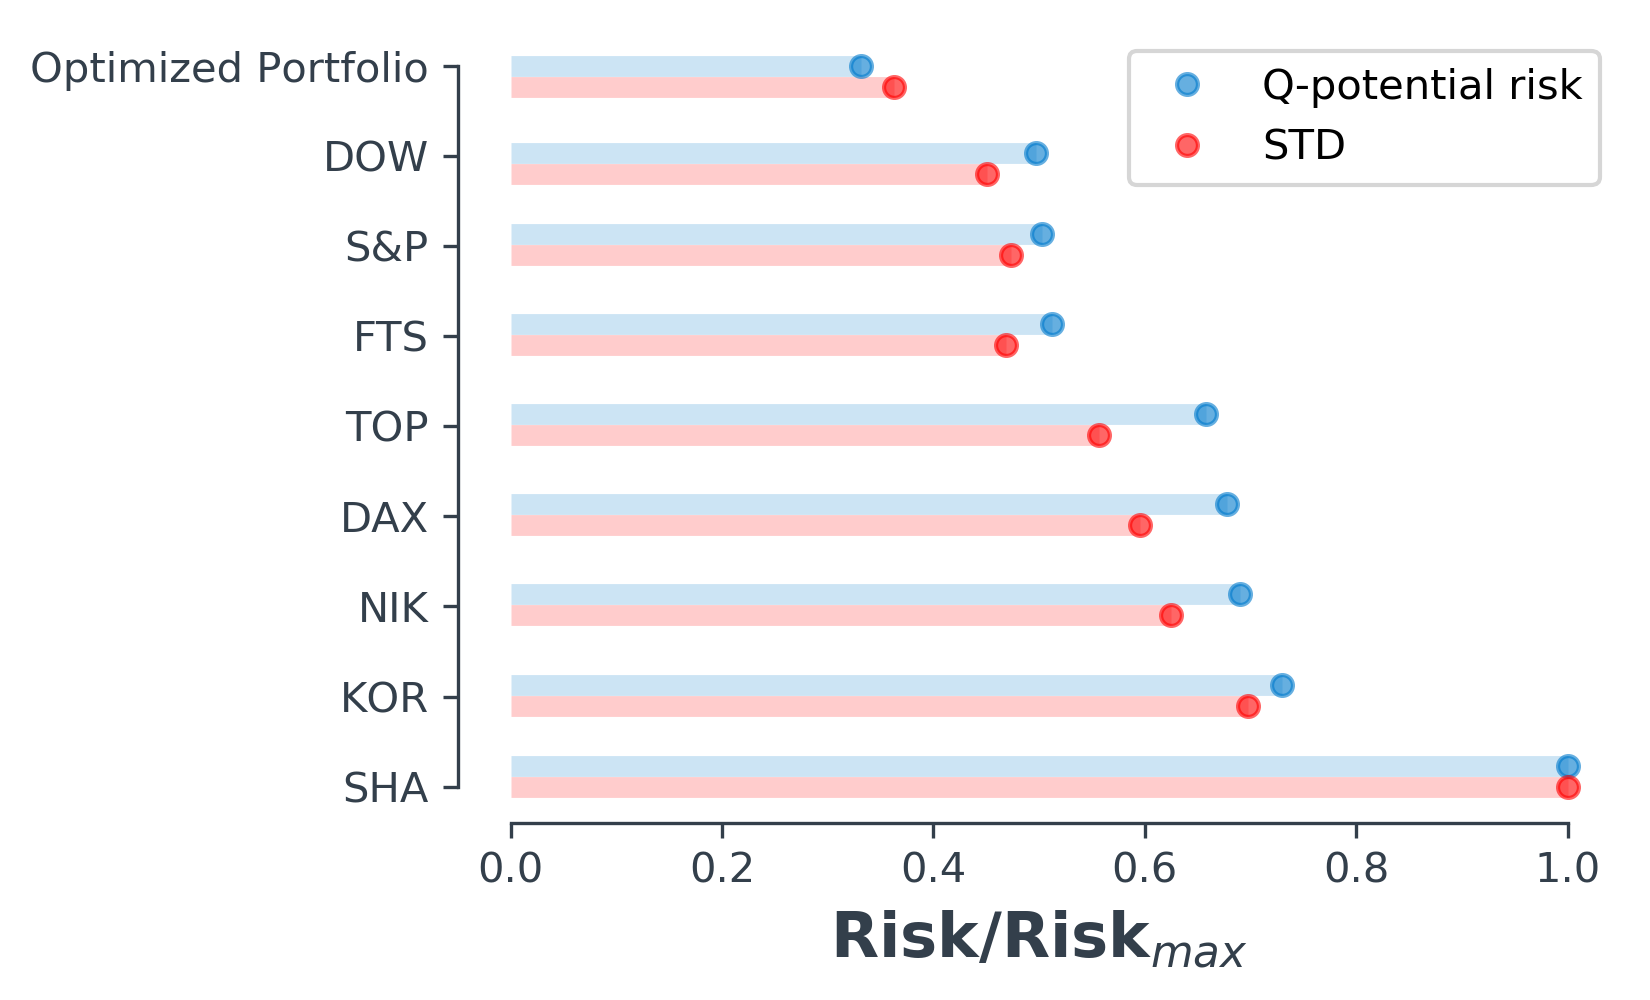
\includegraphics[width=\textwidth]{/home/hossein4527/MEGA/MEGAsync/Commit/University-Projects/MSc_Thesis/plots/fig1.png}
	\caption{سری زمانی قیمت شاخص S\&P500}
	\label{fig:1}
\end{figure}
\begin{figure}[ptb]
	\centering
	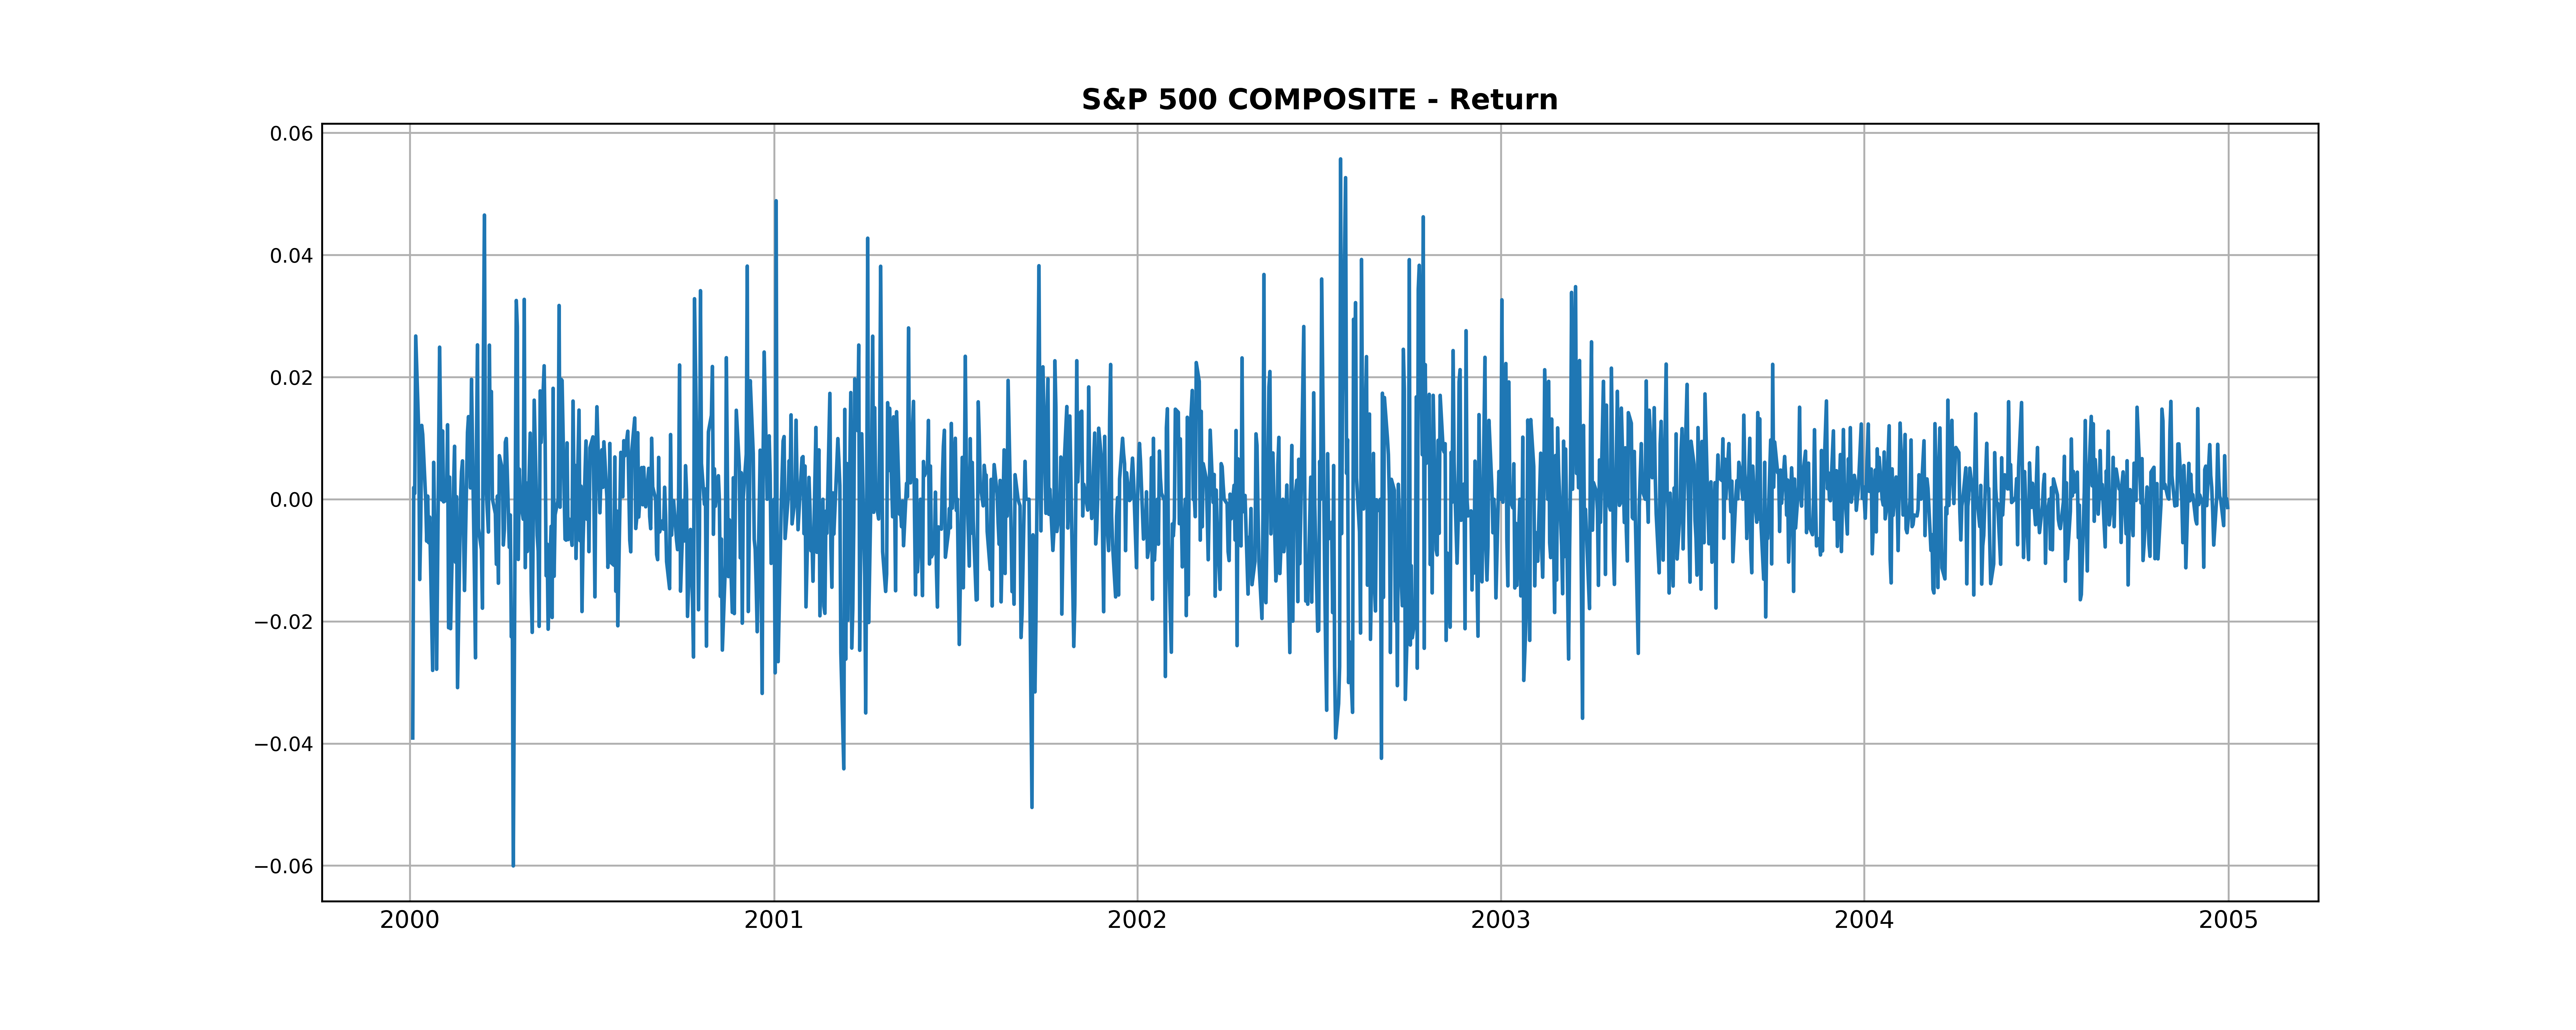
\includegraphics[width=\textwidth]{/home/hossein4527/MEGA/MEGAsync/Commit/University-Projects/MSc_Thesis/plots/fig2.png}
	\caption{سری زمانی سود شاخص S\&P500}
	\label{fig:2}
\end{figure}
با توجه به این که داده های موجود در شکل 
\ref{fig:2}
بر حسب درصد جایگذاری شده اند، خواننده های مختلف به اتفاق آرا می توانند راجع به تک تک نقاط موجود در نمودار با یک زبان صحبت کنند.
برای محاسبه پتانسیل کوانتومی حاکم بر سود و زیان بازار 
S\&P500
در بازه مشخص شده تنها یک قدم باقیست و آن هم محاسبه تابع توزیع $r(t)$، که همان پارامتر $R$ موجود در معادله 
\ref{eq:3.2}
است. برای محاسبه این پارامتر از کتابخوانه سای پای موجود در زبان پایتون کمک میگیریم. اگر برای داده های سود موجود در شکل 
\ref{fig:2}
تابع توزیع رسم کنیم به شکل
\ref{fig:3}
میرسیم.
\begin{figure}[ptb]
	\centering
	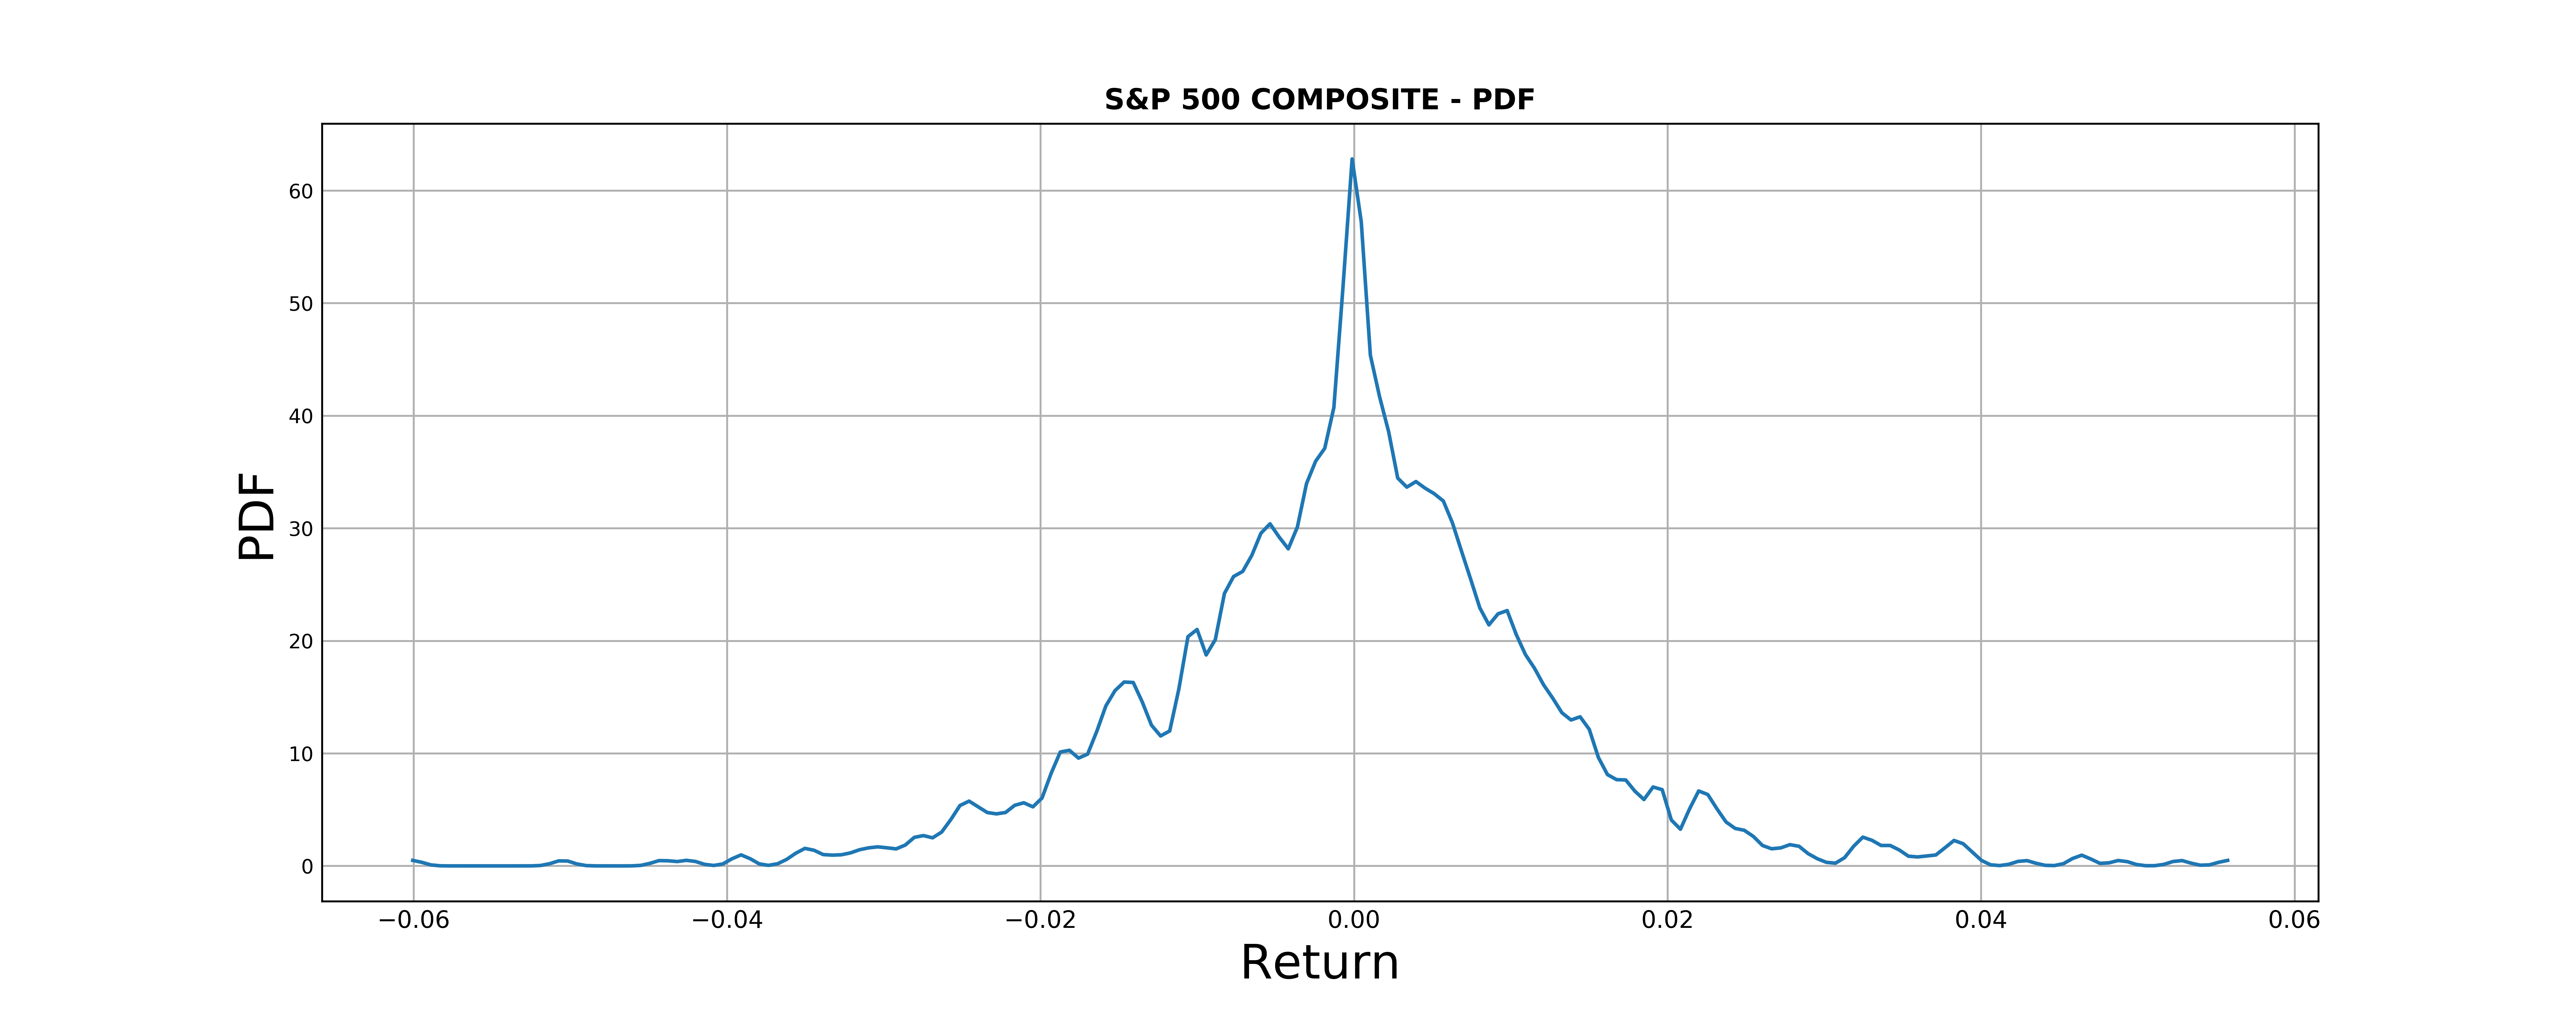
\includegraphics[width=\textwidth]{/home/hossein4527/MEGA/MEGAsync/Commit/University-Projects/MSc_Thesis/plots/fig3.png}
	\caption{تابع توزیع احتمال سود شاخص S\&P500}
	\label{fig:3}
\end{figure}
\newpage
اینک با داشتن پارامتر $R$ می توان برای محاسبه پتانسیل کوانتومی $Q$ اقدام کرد.  در مسیر این محاسبه تنها کافیست از داده های مربوط به تابع توزیع متتغیر $r$ دوبار نسبت به $r$ مشتق بگیریم و نتیجه نهایی را بر خود تابع توزیع، $R$، تقسیم کنیم. برای این کار از کتابخوانه های سای پای و نام پای موجود در زبان برنامه نویسی پایتون کمک میگیریم. شکل
\ref{fig:4}
رفتار پتانسیل کوانتومی حاکم بر بازار 
$S\&P500$
را برای بازه ۵ ساله بین سال های ۲۰۰۰ تا ۲۰۰۵ نشان می دهد. همانطور که در 
\ref{fig:4}
پیداست محور افقی بیانگر میزان سود بازار
$S\&P500$
و محور عمودی بیانگر اندازه ی پتانسیل کوانتومی حاکم بر این بازار در مقادیر مختلف مورد نظر سود است. خواننده با دید اول شهودی نسبت به حضور دو دیواره ی پتانسیلی بزرگ در انتهای مقادیر مثبت و منفی سود پیدا خواهد کرد. حضور این دو دیواره حاکی از آن است که نیرویی درست مشابه نیروی پتانسیل کوانتومی در مکانیک بوهمی در این بازه ۵ ساله از تخطی های سود و زیان بازار 
$S\&P500$
از مقادیری خاص ممانعت می کند. این مقادیر در شکل با علامت قرمز مشخص شده و همان جاییست که مقدار پتانسیل بسیار بزرگ تر از دیگر مقادیر خود است. شکل 
\ref{fig:4}
پتانسیل کوانتومی حاکم بر داده های روزانه شاخص بازار 
$S\&P500$
است و در شکل های 
[\ref{fig:5}-\ref{fig:7}]
همین پتانسیل را برای داده های هفتگی، ماهانه و فصلی میتوان یافت.

\begin{figure}[ptb]
	\centering
	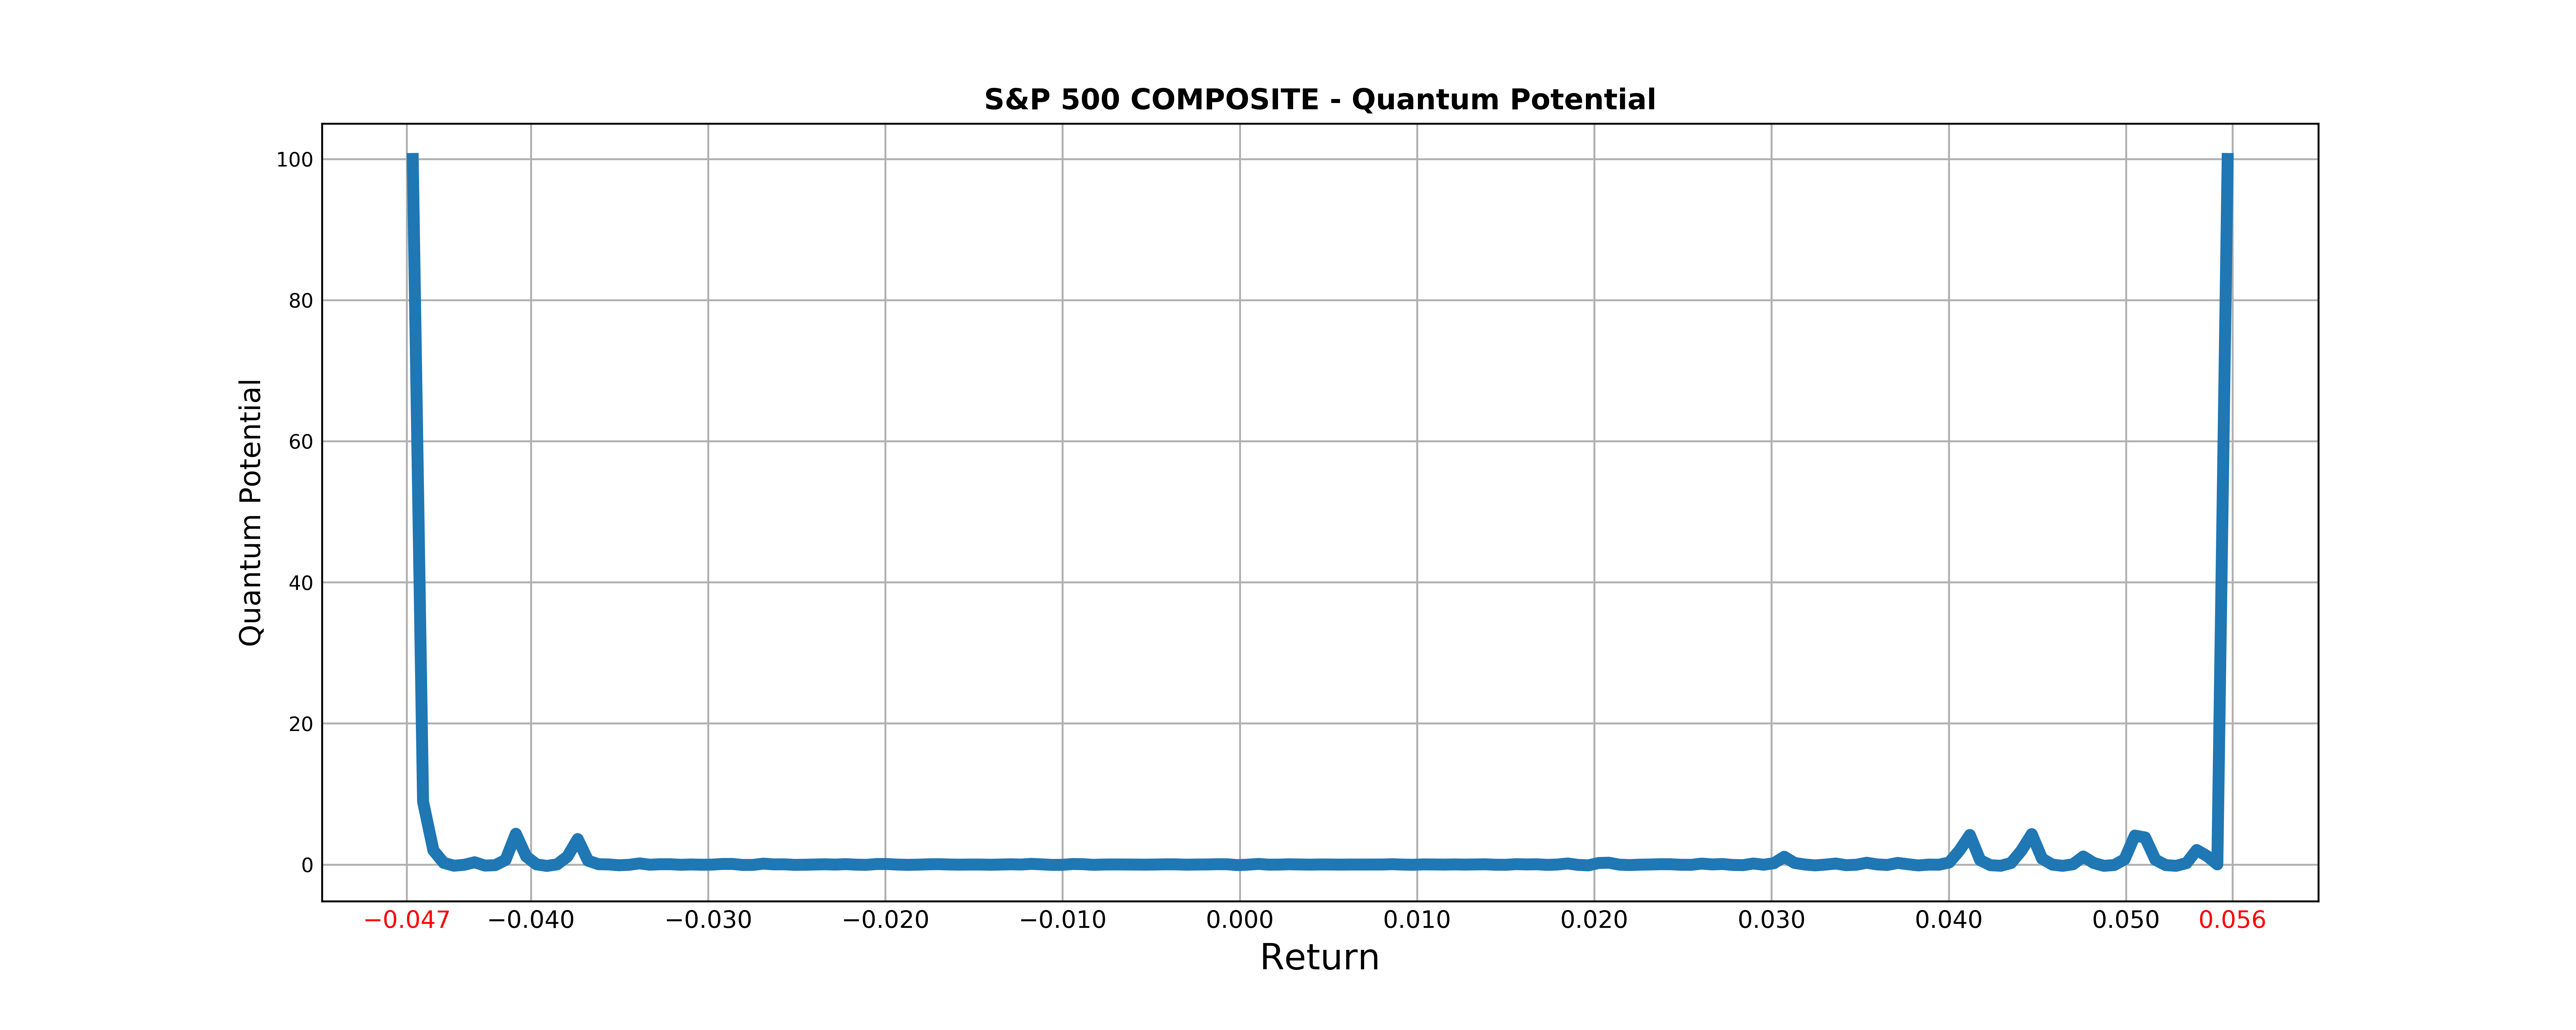
\includegraphics[width=\textwidth]{/home/hossein4527/MEGA/MEGAsync/Commit/University-Projects/MSc_Thesis/plots/fig4.png}
	\caption{پتانسیل کوانتومی حاکم بر داده های روزانه بازار S\&P500}
	\label{fig:4}
\end{figure}

\begin{figure}[ptb]
	\centering
	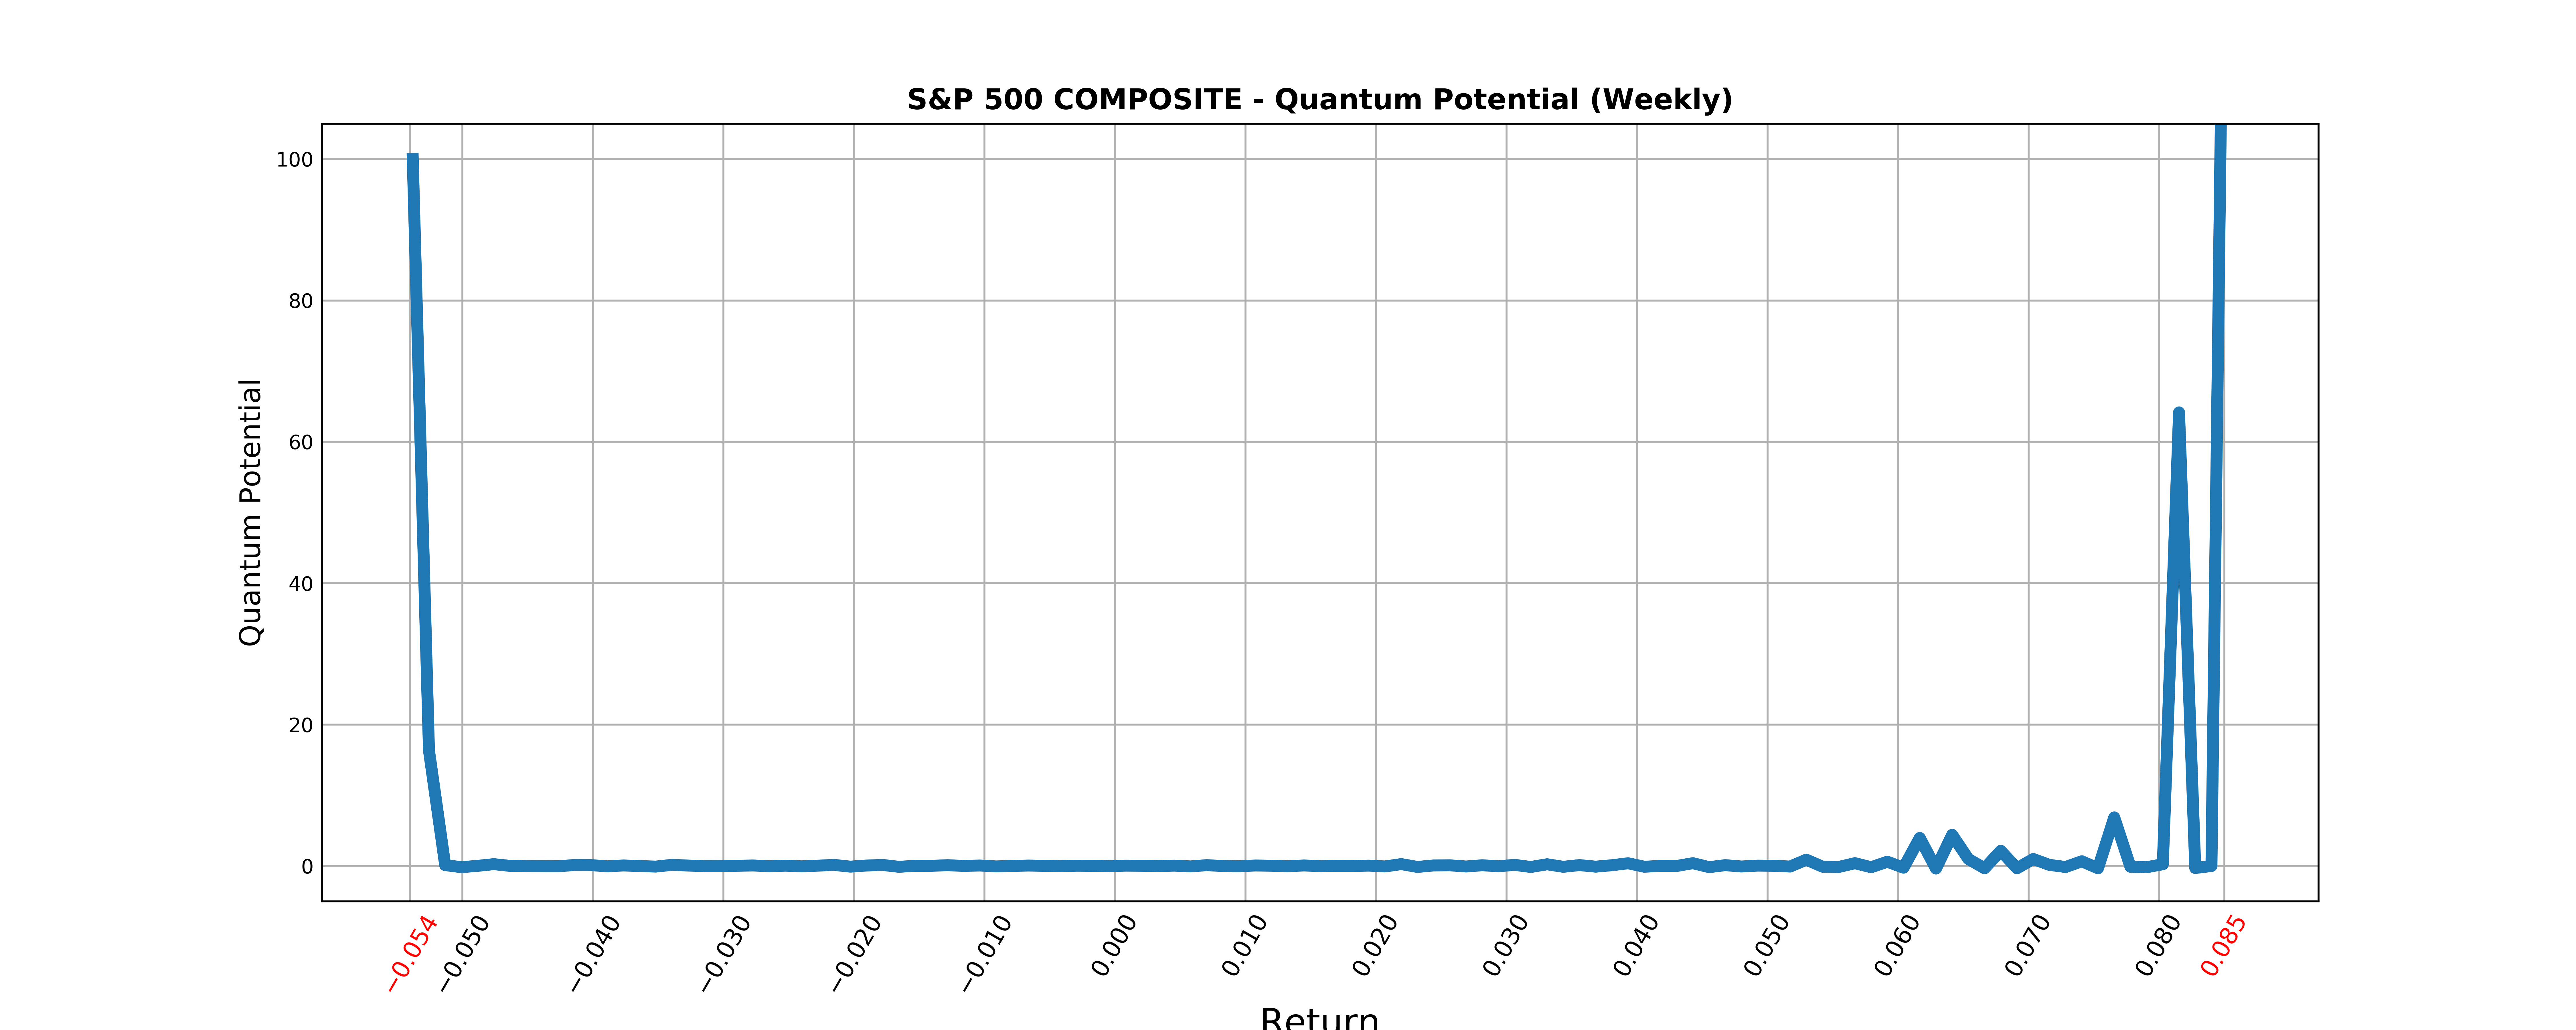
\includegraphics[width=\textwidth]{/home/hossein4527/MEGA/MEGAsync/Commit/University-Projects/MSc_Thesis/plots/fig5.png}
	\caption{پتانسیل کوانتومی حاکم بر داده های هفتگی بازار S\&P500}
	\label{fig:5}
\end{figure}

\begin{figure}[ptb]
	\centering
	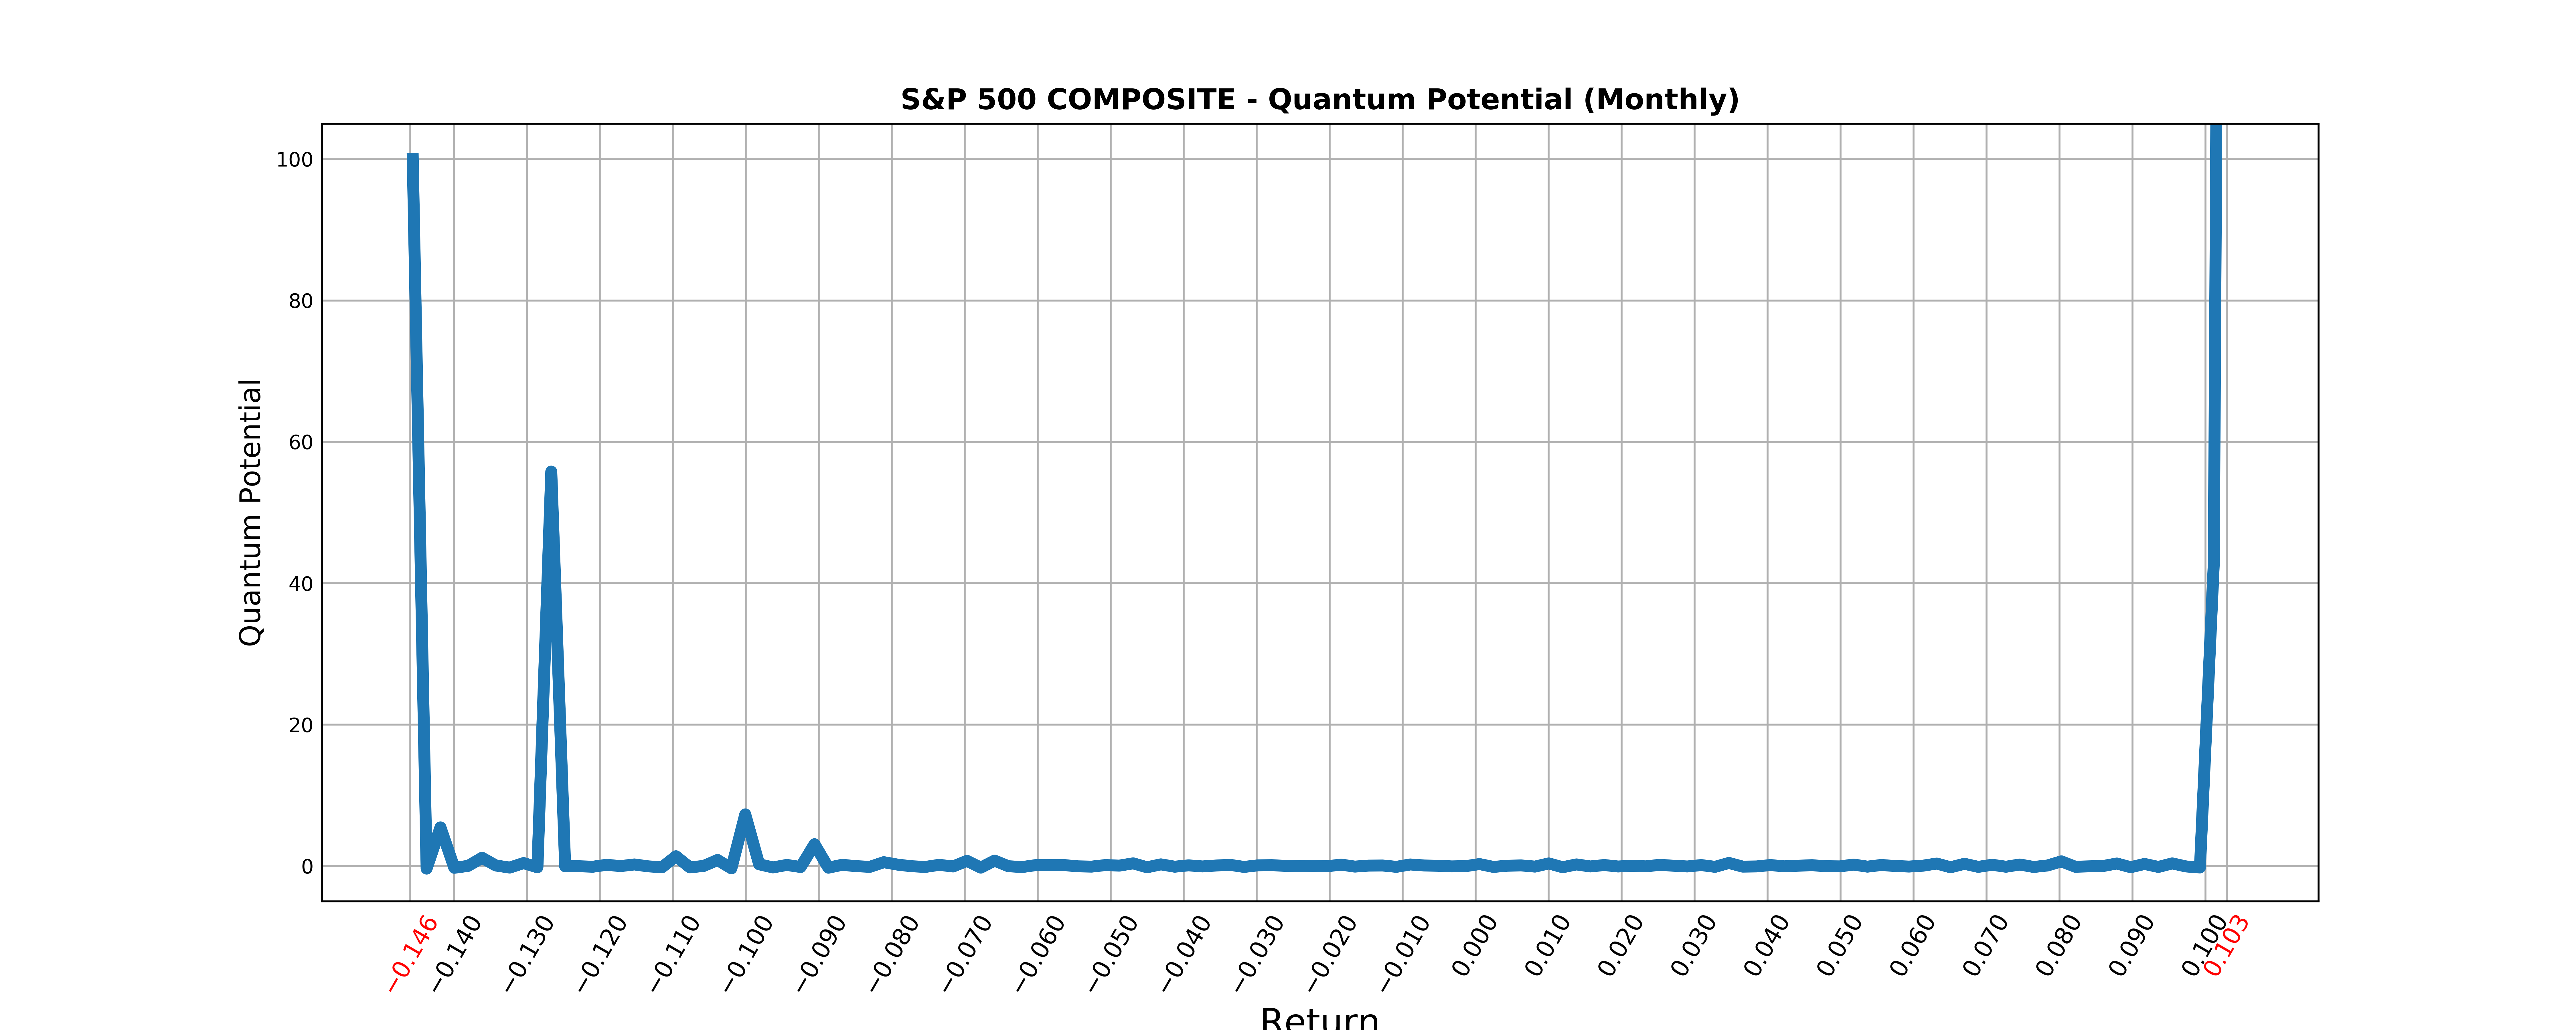
\includegraphics[width=\textwidth]{/home/hossein4527/MEGA/MEGAsync/Commit/University-Projects/MSc_Thesis/plots/fig6.png}
	\caption{پتانسیل کوانتومی حاکم بر داده های ماهانه بازار S\&P500}
	\label{fig:6}
\end{figure}

\begin{figure}[ptb]
	\centering
	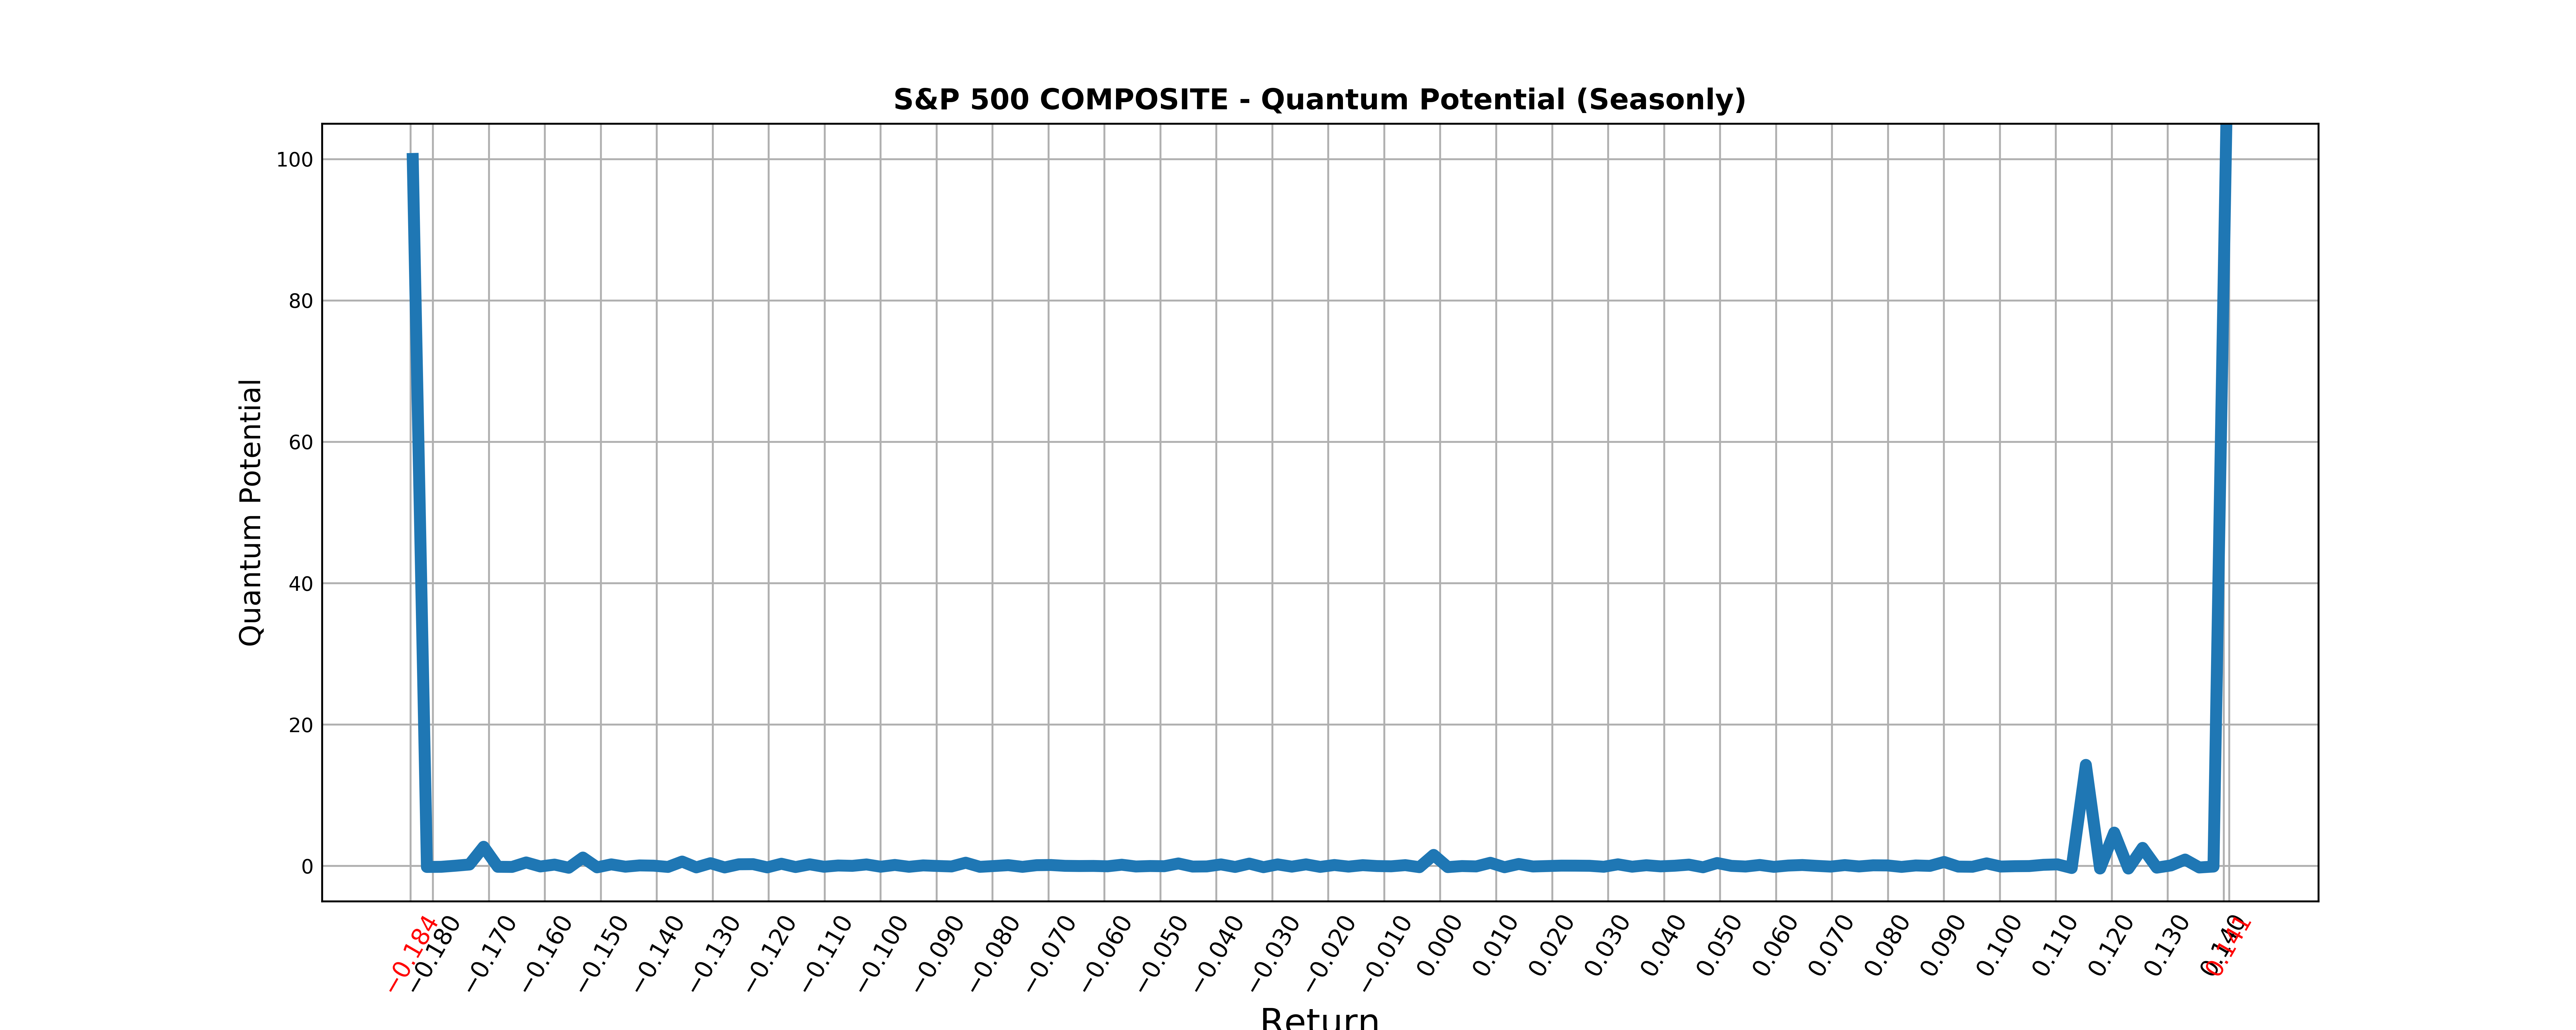
\includegraphics[width=\textwidth]{/home/hossein4527/MEGA/MEGAsync/Commit/University-Projects/MSc_Thesis/plots/fig7.png}
	\caption{پتانسیل کوانتومی حاکم بر داده های فصلی بازار S\&P500}
	\label{fig:7}
\end{figure}
\newpage
تا اینجای کار به نحوه محاسبه و نمایش پتانسیل کوانتومی جاکم بر یک بازار پرداختیم و دیدیم چگونه میتوان آن را از روی داده های قیمتی یک بازار محاسبه کرد. در اینجا نیاز است که تحلیلی بر شکل های نمایش داده شده انجام شود و تفسیر آن ها به صورت تک به تک و همچنین مقایسه آنها با یکدیگر انجام شود. 

همانظور که در شکل 
\ref{fig:4}
و همچنین در شکل های 
[\ref{fig:5}-\ref{fig:7}]
پیداست، دیواره  هایی از جنس پتانسیل سد معبری روی محور سود و زیان برای بازار مورد مشاهده وجود دارند.  این دیواره ها برای بازه های زمانی سرمایه گذاری جا به جا می شوند و اجازه ی سود دهی بیشتر و یا کمتر را نسبت به بازه های دیگر صادر می کنند. برای داده های روزانه شکل
\ref{fig:4}
این مکان این دیواره در قسمت سود دهی مثبت بزرگ تر از مکان این دیواره در قسمت سود دهی منفی است و همین امر حاکی از آن است که در بازه ۵ ساله مشاهده شده بازار
$S\&P500$، 
سری زمانی روزانه سود دهی این بازار تمایل بیشتری به سود دهی نسبت به ضرر دهی دارد. این امر در شکل 
\ref{fig:5}
که مربوط به داده های هفتگی است هم قابل مشاهده است. برای سرمایه گذاری های بلند مدت تر در بازار 
$S\&P500$
در بازه زمانی ۵ ساله ۲۰۰۰-۲۰۰۵ چه در مقیاس ماهانه و چه در مقیاس فصلی، در شکل های 
\ref{fig:6}
و 
\ref{fig:7}
قابل مشاهده است که پتانسیل کواننتومی حاکم اجازه دسترسی به فضای زیان بیشتری نسبت به سود صادر کرده است.
با کمک همین امر میتوان در سرمایه گذاری های مدت معلوم در هر بازاری یک حس اولیه به جنس بازار مورد نظر پیدا کرد. برای اطلاعات بیشتر در فصل بعدی به صورت جزئی تر سخن خواهیم گفت. در اینجا به همین امر کفایت می دهیم که پتانسیل کوانتومی یک بعدی حاکم بر یک بازار نقشی چون کنترل کننده رفتار های یاغی بازار مورد نظر و محدود کردن فضای سود و ضرر بازار مورد نظر دارد. در بخش بعدی به پتانسیل کوانتومی حاکم بر دو بازار و نحوه محاسبه آن می پردازیم.

\section{پتانسیل کوانتومی مشترک حاکم بر سود و زیان دو بازار}
در بخش قبلی به نحوه محاسبه پتانسیل کوانتومی یک بعدی جاکم بر سود و زیان یک بازار پرداختیم و نشان دادیم چگونه این پتانسیل با محدود کردن فضای سود و زیان قابل دسترس آن بازار، از تخطی های خارج از محدوده مجاز آن جلوگیری می کند. در این بخش میخواهیم به محاسبه همین مفهوم ولی این بار برای دو بازار بپردازیم و تلاش کنیم به این سوال جواب دهیم که آیا پتانسیل کوانتومی مشترک محاسبه شده توسط تابع توزیع مشترک دو بازار نیز همانند پتانسیل یک بعدی فضای سود و زیان مشترک دو بازار را محدود می کند؟ برای رسیدن به این مفهوم پله به پله به محاسبه پتانسیل مشترک دو بازار می پردازیم.

 برای این کار ابتدا لازم است معادله شرودینگر نوشته شده برای یک ذره در معادله 
 \ref{eq:3.2}
 را برای چند ذره(دو ذره در اینجا) تعمیم دهیم و صورت پتانسیل کوانتومی تعمیم یافته برای چند(دو) ذره را بیابیم. از آنجایی که پتانسیل خارجی نقشی در پتانسیل کوانتومی ندارد و پتانسیل کوانتومی تنها به خواص خود ذره بستگی دارد و با توجه به معادله 
 \ref{eq:3.3}
 
 \begin{equation}
 i \hbar \frac{\partial\psi(q_1,q_2,t)}{\partial t} =\left(-\frac{\hbar^2}{2m_1}{\nabla_1^2}-\frac{\hbar^2}{2m_2}{\nabla_2^2} \right)\psi(q_1,q_2,t)+V(q_1,q_2,t)\psi(q_1,q_2,t) ،
 \label{eq:3.3}
 \end{equation}
 معادله شرودینگر جدای از قسمت پتانسیل خارجی اش در اضافه شدن ذرات جدید خطی است. پس به راحتی می توان پتانسیل کوانتومی تعمیم یافته برای $n$ ذره را به صورت معادله
 \ref{eq:3.4}
 محاسبه کرد.
\begin{equation}
Q(q_{1},q_{2},...,q_{n})=-\frac{\hbar}{2R(q_{1},q_{2},...,q_{n})}\sum
_{i=1}^{n}\frac{\nabla_i^2}{m_{i}}R(q_{1}
,q_{2},...,q_{n}).
 \label{eq:3.4}
\end{equation}
در معادله 
\ref{eq:3.4}،
$\nabla_i^2$
لاپلاسین نسبت به مختصات ذره ی $i$ ام است.
اینک با در دست داشتن صورت کلی پتانسیل کوانتومی برای چند ذره، می توان این پارامتر را برای هر تعداد بازار دلخواه محاسبه کرد. در این پایان نامه برای سادگی کار به محاسبه پتانسیل کوانتومی مشترک بین دو بازار می پردازیم. طبق معادله
\ref{eq:3.4}
پتانسیل کوانتومی برای چنین سیستمی به صورت زیر محاسبه می شود:
\begin{equation}
Q(q_{1},q_{2})=-\frac{\hbar}{2R(q_{1},q_{2})}\left(\frac{\nabla_1^2}{m_{1}}R(q_{1}
,q_{2}) + \frac{\nabla_2^2}{m_{2}}R(q_{1},q_{2})\right).
\label{eq:3.5}
\end{equation}
معادله
\ref{eq:3.5}
را می توان به شکل خلاصه تر زیر نوشت:
\begin{equation}
Q(q_{1},q_{2})=-\frac{\hbar}{2}\left(\frac{Q_{q_1:q_2}}{m_{1}} + \frac{Q_{q_2:q_1}}{m_{2}}\right)،
\label{eq:3.6}
\end{equation}
که در آن با توجه به اینکه تنها مختصه ذره اول
 $\vec{q_1} = r_1\hat{r}$ 
 و ذره دوم همانند ذره اول در این کار پایان نامه سود و زیان لگاریتمی در نظر گرفته شده است، 
 $Q_{q_1:q_2}$
 و
 $Q_{q_2:q_1}$
 به صورت زیر محاسبه خواهند شد:

\begin{equation}
Q_{r_1:r_2} =\frac{1}{R(r_1,r_2)} \nabla_1^2 R(r_{1},r_{2} ) =\frac{1}{R(r_1,r_2)} \frac{\partial^2 R(r_1,r_2)}{\partial r_1^2}،
\label{eq:3.7}
\end{equation}

\begin{equation}
Q_{r_2:r_1} =\frac{1}{R(r_1,r_2)} \nabla_2^2 R(r_{1},r_{2} ) =\frac{1}{R(r_1,r_2)} \frac{\partial^2 R(r_1,r_2)}{\partial r_2^2}.
\label{eq:3.8}
\end{equation}
پتانسیل های معادلات 
\ref{eq:3.7}
و
\ref{eq:3.8}
 در این کارپتانسیل های کوانتومی شرطی نام گذاری شده اند و هر کدام بیان گر این موضوع هستند که پتانسیل یک بعدی هر کدام از این ذرات(بازارها) در حضور ذره(بازار) دیگر چگونه عمل خواهند کرد و میزان تاثیر پذیری این پتانسیل ها از یکدیگر چه مقدار است.
برای محاسبه هر کدام از پتانسیل های معادلات 
\ref{eq:3.7}
و
\ref{eq:3.8}
تنها یک قدم باقی است و آن هم محاسبه تابع توزیع مشترک سود و زیان هر دو بازار دلخواه
$R(r_1,r_2)$
است. قبل از اینکه به محاسبه این کمیت برای داده های واقعی بپردازیم، میخواهیم به مدلی بپردازیم که در آن تصور شده است که تابع توزیع مشترک هر دو بازار از تابع گاوسی دو بعدی پیروی می کند و برای این مدل به محاسبه پتانسیل های کوانتومی بحث شده در این بخش می پردازیم. برای مشاهده نتیجه این کار بخش بعدی را مطالعه بفرمایید.
\subsection{ارائه طرح پیشنهادی تابع توزیع گاوسی}
در بخش قبل به ریاضیات مورد نیاز برای محاسبه پتانسیل کوانتومی دو بعدی مشترک برای هر دو ذره یا دو بازار دلخواه پرداختیم. در این بخش تنها به کمک معادلات
\ref{eq:3.7}
و
\ref{eq:3.8}
به ارائه طرحی میپردازیم که در آن 
$R(r_1,r_2)$
به کار رفته در معادلات فوق از تابعی گاوسی طبعیت می کند. این  تابع گاوسی در کلی ترین حالت ممکن خود به صورت زیر قابل بیان است:
\begin{equation}
R(r_1,r_2) \propto \exp\left( -\frac{1}{2} \left( (\frac{r_1}{\sigma_1})^2 + (\frac{r_2}{\sigma_2})^2 +2\rho(\frac{r_1}{\sigma_1})(\frac{r_2}{\sigma_2})\right)\right)،
\label{eq:3.9}
\end{equation}
که در آن 
$\sigma_i$
ها واریانس سری زمانی 
$r_i$
ها هستند و 
$\rho$
میزان همبستگی سری های زمانی 
$r_i$
ها است.
برای ادامه نیاز است که پتانسیل های معادلات 
\ref{eq:3.7}
و
\ref{eq:3.8}
را برای این تابع توزیع بخصوص محاسبه کنیم.
هر کدام از این معادلات به راحتی و تنها یک مشتق گیری و ساده سازی ساده و پتانسیل کوانتومی کل نیز از معادله 
\ref{eq:3.6}
به صورت زیر بدست می آید:

\begin{equation}
Q_{r_1:r_2} = \frac{1}{R(r_1,r_2)} \frac{\partial^2 R(r_1,r_2)}{\partial r_1^2} = \frac{1}{\sigma_1^2}\left(\left(\frac{r_1}{\sigma_1} + \rho\frac{r_2}{\sigma_2}\right)^2-1\right)
\label{eq:3.10}
\end{equation}

\begin{equation}
Q_{r_2:r_1}  = \frac{1}{R(r_1,r_2)}\frac{\partial^2 R(r_1,r_2)}{\partial r_2^2}  = \frac{1}{\sigma_2^2}\left(\left(\frac{r_2}{\sigma_2} + \rho\frac{r_1}{\sigma_1}\right)^2-1\right).
\label{eq:3.11}
\end{equation}
در معادلات 
\ref{eq:3.10}
و
\ref{eq:3.11}،
پتانسیل های کوانتومی شرطی آورده شده اند و در آن ها 
$r_i$
ها متغیر مستقل مختصه بازار $i$ ام هستند که در این پایان نامه، سود و زیان لگاریتمی بازار $i$ام در نظر گرفته شده اند.

قدم بعدی آن است که پتانسیل های 
$Q_{r_2:r_1}$
و
$Q_{r_1:r_2}$
را طبق معادلات 
\ref{eq:3.10}
و
\ref{eq:3.11}
برای مقادیر مختلف 
$r_1$
و
$r_2$
حساب کنیم. در این مسیر 
$r_1$
و
$r_2$
مختصات هستند و متغیر های 
$\sigma_1$،
$\sigma_2$
و
$\rho$
به صورت دستی و مقادیر مختلفی انتخاب می شوند. با توجه به انتخاب های مختلف از مجموعه انتخاب های در دسترس،  بازارهای دوتایی با مشخصه های مختلفی ساخته خواهند شد. 
$\rho$
که میزانی بر همبستگی دو بازار است و همواره مقداری بین 
$-1$
و 
$1$
دارد، می تواند با کم یا زیاد اختیار شدنش وابستگی دو بازار ساختگی را کم و زیاد کند. 
این متغیر در کنار 
$\sigma_i$
ها که در معادله 
\ref{eq:3.9}
به خوبی قابل مشاهده هستند، می توانند تقارن تابع توزیع
$R(r_1,r_2)$
را برهم زنند و به پشتوانه آن باعث تغییراتی در پتانسیل های کوانتومی شوند. برای بررسی این تغییرات و تفسیر آن ها و همینطور محاسبه پتانسیل کوانتومی کل و تفسیر آن در بخش های بعدی با انتخاب مقادیر مشخصی از سه متغیر
$\sigma_1$،
$\sigma_2$
و
$\rho$
به این سوال پاسخ خواهیم داد که آیا پتانسیل کوانتومی(چه از نظر هندسی و چه از نظر مقداری) می تواند تفاسیر خود را در کنار ابزار عمل های مکانیک آماری در این حوزه از علم دهد و آیا شامل برتری خاصی می شود یا خیر؟ برای یافتن این موضوع تا چند بخش بعدی با ما همراه باشید.
\subsection{
بررسی متغیر 
$\rho$
 برای بازارهای با واریانس یکسان،
$\sigma_1 = \sigma_2$
}
بیاین اجازه دهیم 
$\rho$
مقادیری بین صفر و یک اختیار کند در حالی که 
$\sigma_1 = \sigma_2$،
و ببینیم توابع توزیع و پتانسیل های شرطی و مجموع آنها که پتانسیل کل است، چگونه رفتار می کنند. شکل 
\ref{fig:1t}
و 
\ref{fig:2t}
از زاویه ای متفاوت این توابع را برای مقادیر مختلفی از ضریب همبستگی دو بازار،
$\rho$
 نشان می دهد. 
  \begin{figure}[tbp]
  	\centering
  	\begin{subfigure}[b]{\textwidth}
  		\renewcommand\thesubfigure{a}
  		\begin{subfigure}[b]{0.24\textwidth}
  			\renewcommand\thesubfigure{i}
  			\centering
  			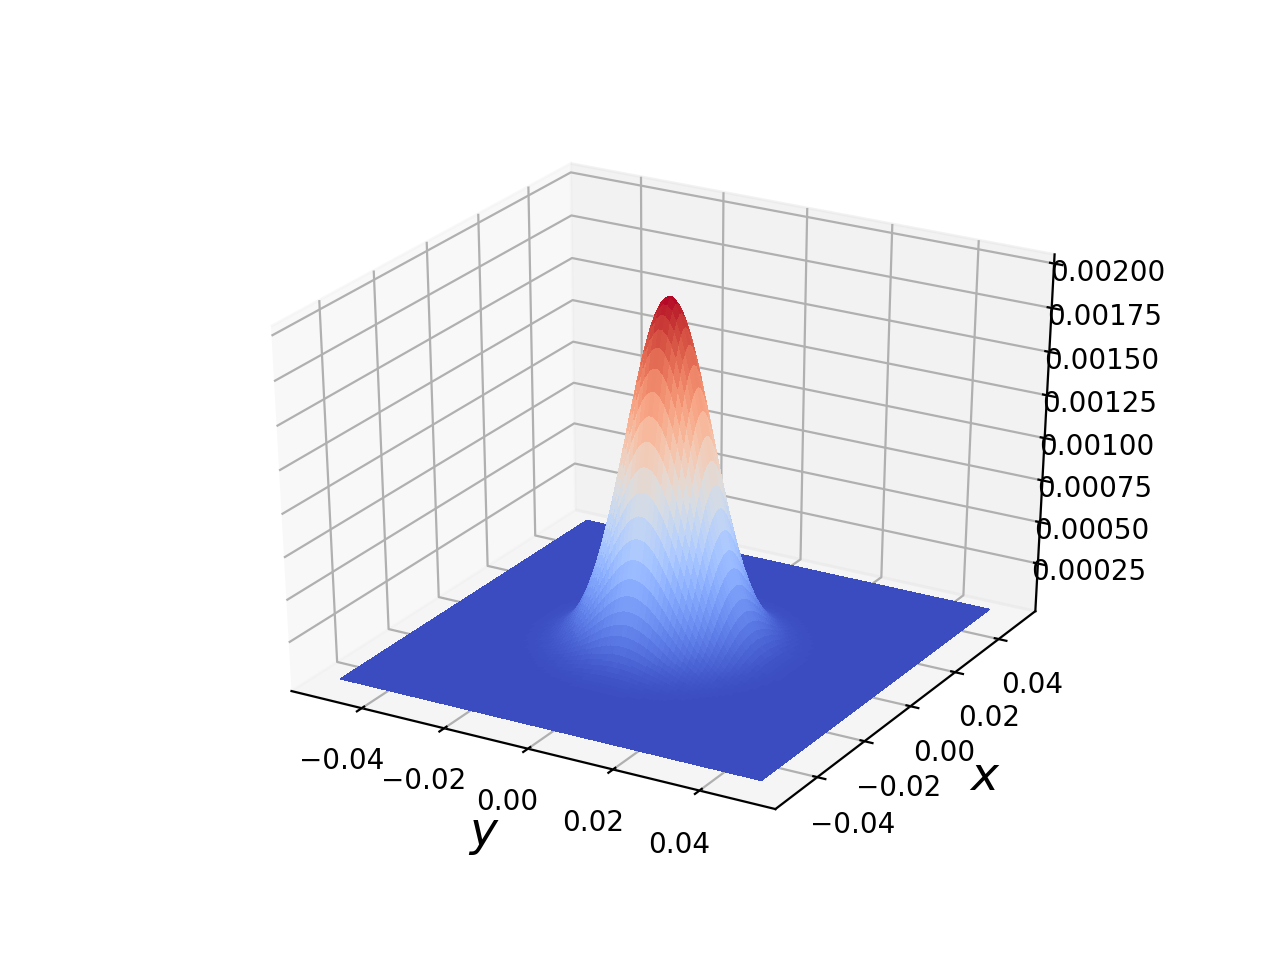
\includegraphics[width=\textwidth]{/home/hossein4527/MEGA/MEGAsync/Commit/University-Projects/MSc_Thesis/plots/Fig:(1a).png}
  			\caption{$Joint PDF$}
  			\label{fig:1.1.1}
  		\end{subfigure}
  		\hfill
  		\begin{subfigure}[b]{0.24\textwidth}
  			\renewcommand\thesubfigure{ii}
  			\centering
  			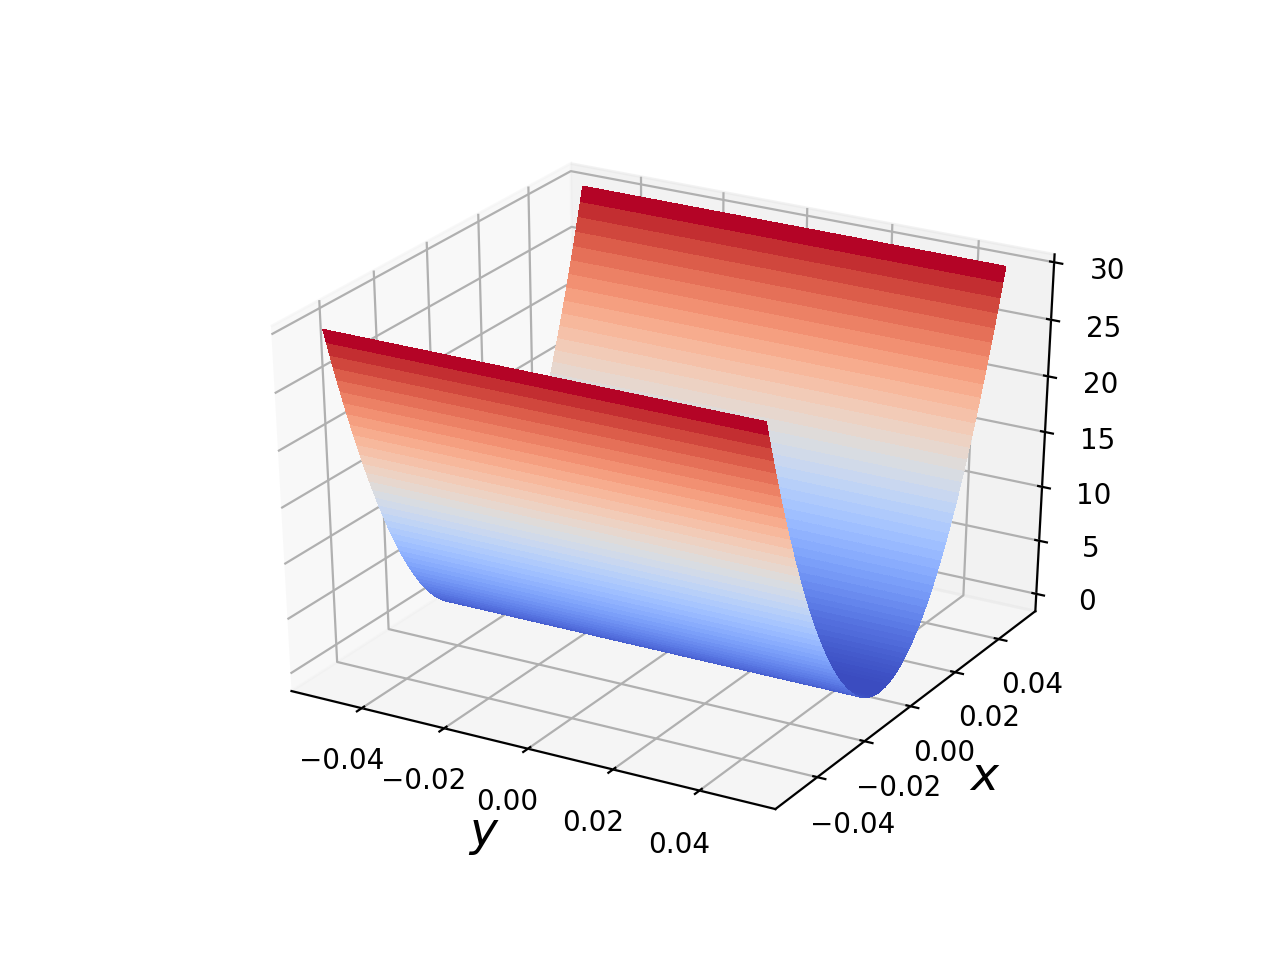
\includegraphics[width=\textwidth]{/home/hossein4527/MEGA/MEGAsync/Commit/University-Projects/MSc_Thesis/plots/Fig:(1b).png}
  			\caption{$Q_{x:y}$}
  			\label{fig:1.1.2}
  		\end{subfigure}
  		\hfill
  		\begin{subfigure}[b]{0.24\textwidth}
  			\renewcommand\thesubfigure{iii}
  			\centering
  			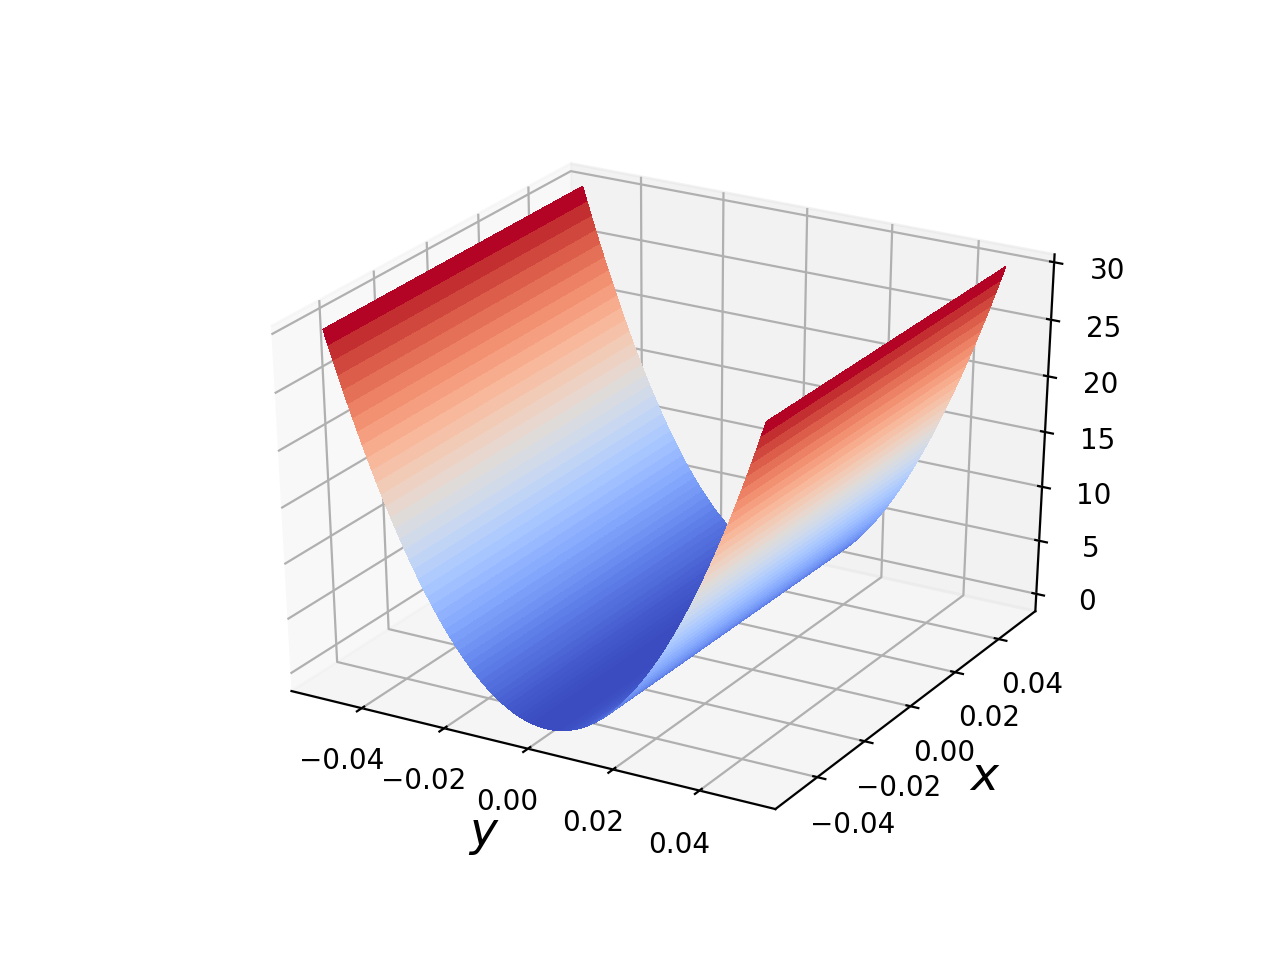
\includegraphics[width=\textwidth]{/home/hossein4527/MEGA/MEGAsync/Commit/University-Projects/MSc_Thesis/plots/Fig:(1c).png}
  			\caption{$Q_{y:x}$}
  			\label{fig:1.1.3}
  		\end{subfigure}
  		\hfill
  		\begin{subfigure}[b]{0.24\textwidth}
  			\renewcommand\thesubfigure{iv}
  			\centering
  			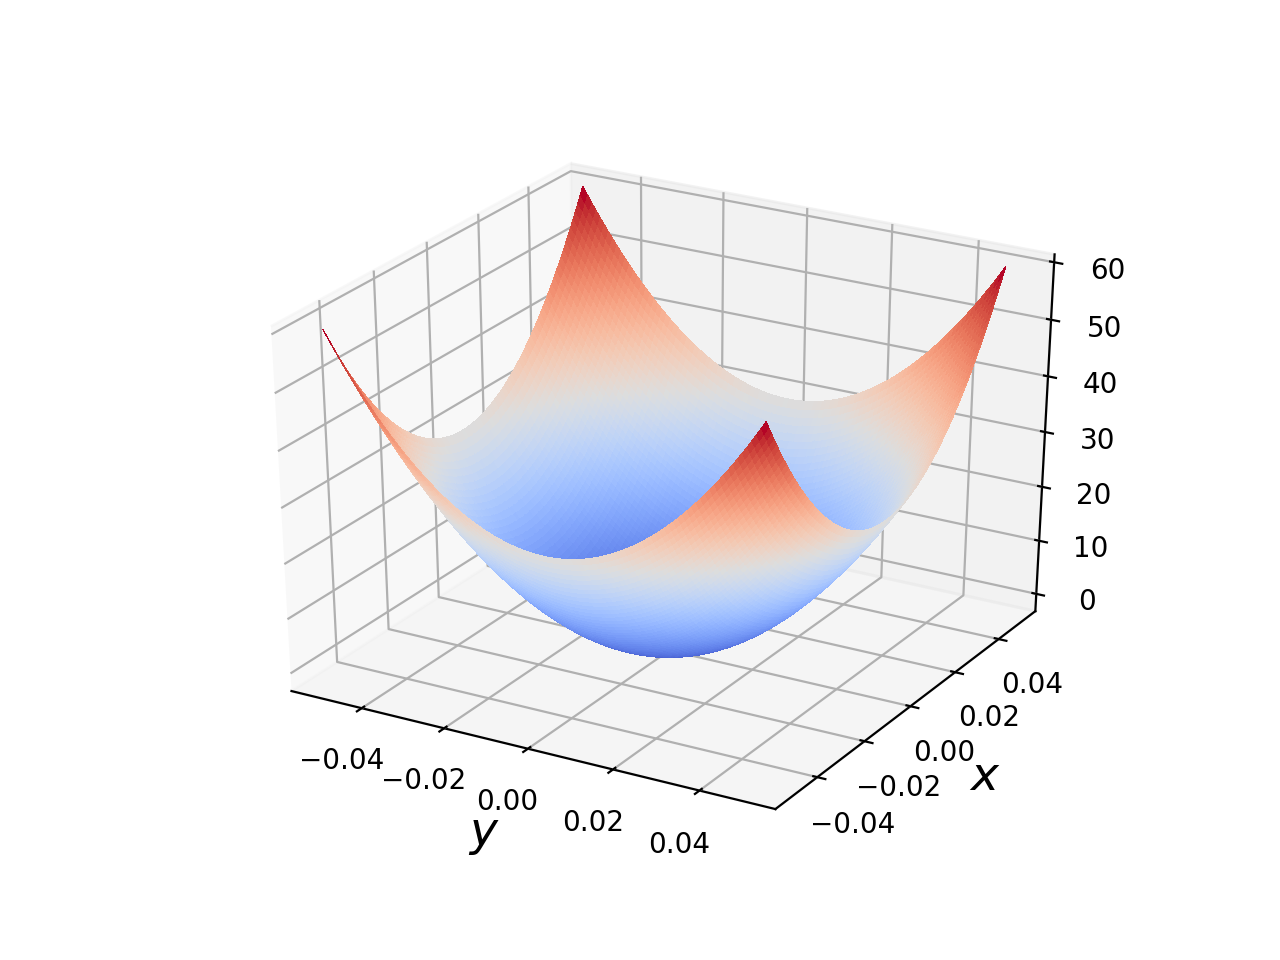
\includegraphics[width=\textwidth]{/home/hossein4527/MEGA/MEGAsync/Commit/University-Projects/MSc_Thesis/plots/Fig:(1d).png}
  			\caption{$Q_{total}$}
  			\label{fig:1.1.4}
  		\end{subfigure}
  		\caption{$\protect\rho =0$ و $\protect\sigma _{x}=\protect\sigma _{y}$}
  		\label{fig:1.1}
  	\end{subfigure}
  	\begin{subfigure}[b]{\textwidth}
  		\renewcommand\thesubfigure{b}
  		\begin{subfigure}[b]{0.24\textwidth}
  			\renewcommand\thesubfigure{i}
  			\centering
  			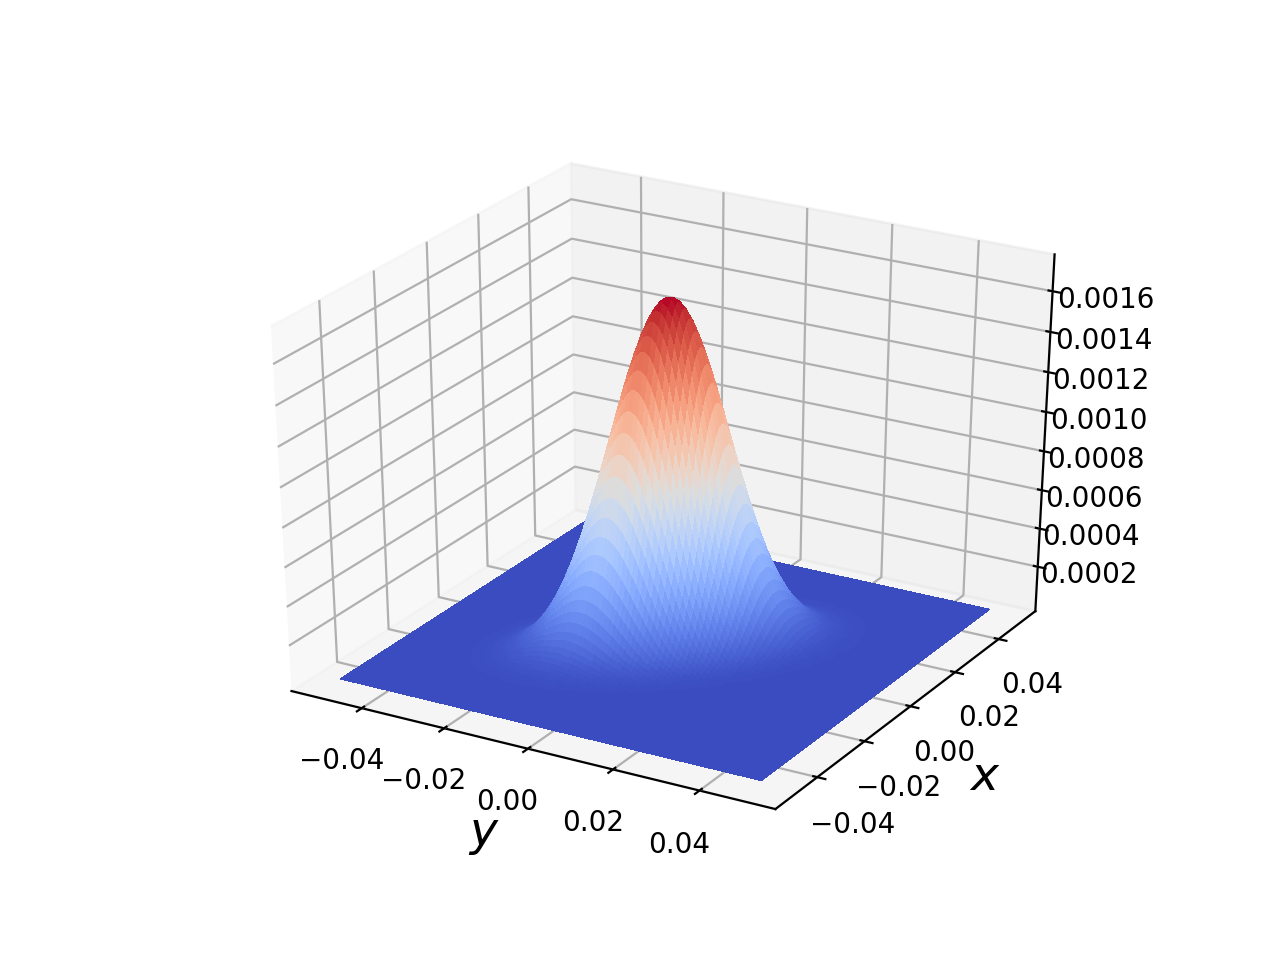
\includegraphics[width=\textwidth]{/home/hossein4527/MEGA/MEGAsync/Commit/University-Projects/MSc_Thesis/plots/Fig:(2a).png}
  			\caption{$Joint PDF$}
  			\label{fig:1.2.1}
  		\end{subfigure}
  		\hfill
  		\begin{subfigure}[b]{0.24\textwidth}
  			\renewcommand\thesubfigure{ii}
  			\centering
  			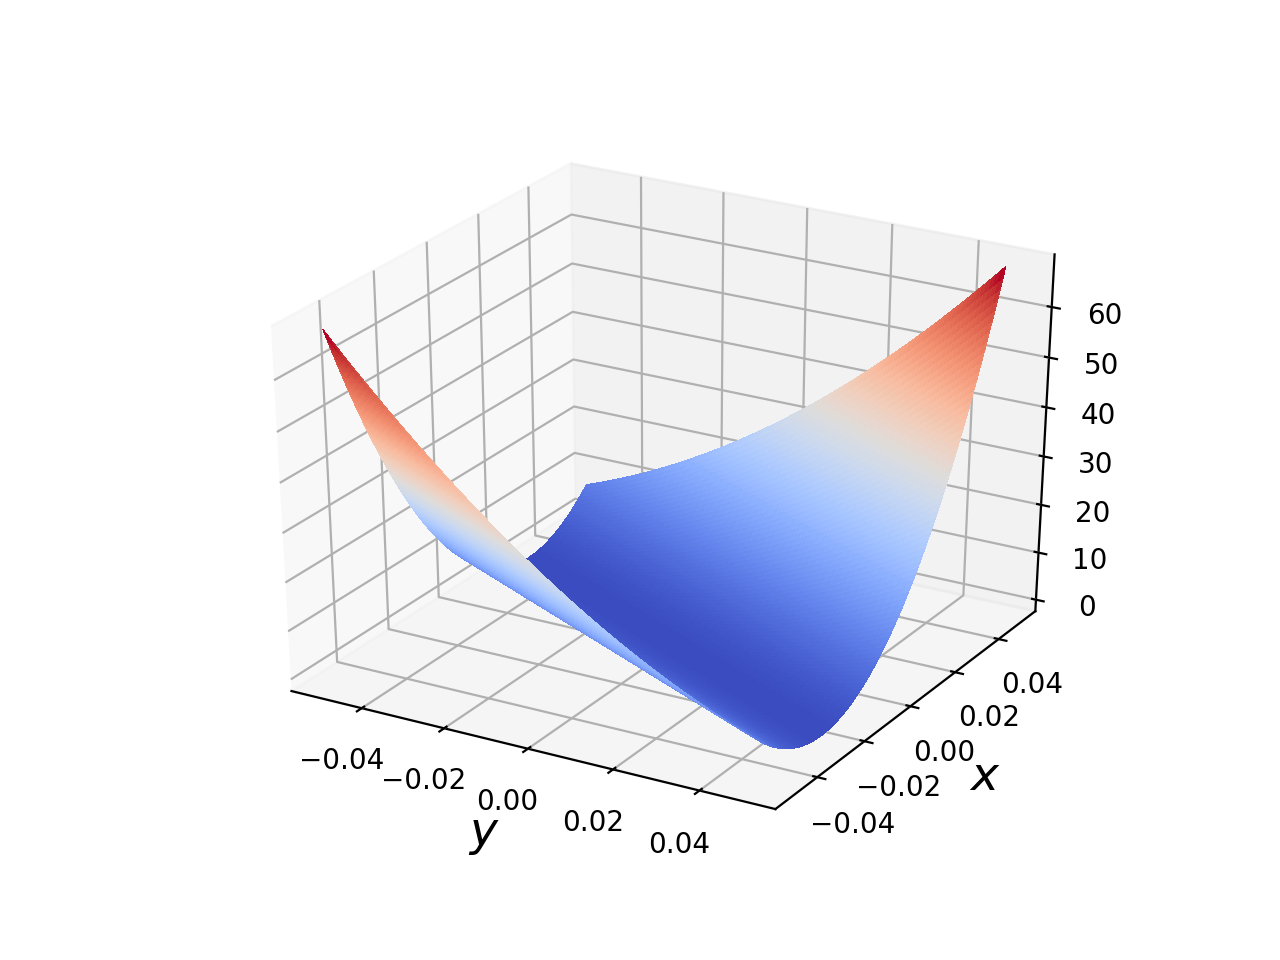
\includegraphics[width=\textwidth]{/home/hossein4527/MEGA/MEGAsync/Commit/University-Projects/MSc_Thesis/plots/Fig:(2b).png}
  			\caption{$Q_{x:y}$}
  			\label{fig:1.2.2}
  		\end{subfigure}
  		\hfill
  		\begin{subfigure}[b]{0.24\textwidth}
  			\renewcommand\thesubfigure{iii}
  			\centering
  			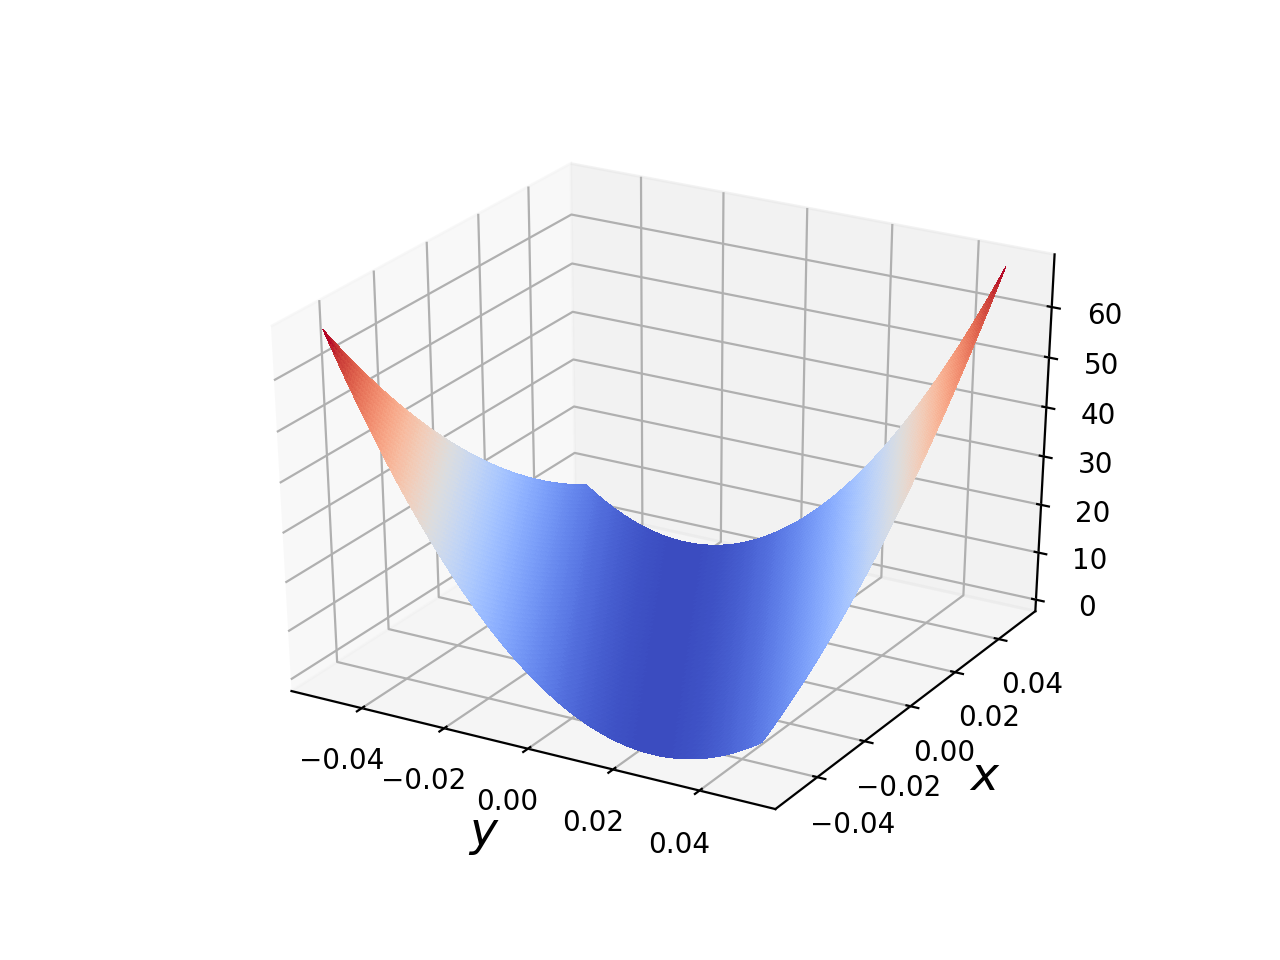
\includegraphics[width=\textwidth]{/home/hossein4527/MEGA/MEGAsync/Commit/University-Projects/MSc_Thesis/plots/Fig:(2c).png}
  			\caption{$Q_{y:x}$}
  			\label{fig:1.2.3}
  		\end{subfigure}
  		\hfill
  		\begin{subfigure}[b]{0.24\textwidth}
  			\renewcommand\thesubfigure{iv}
  			\centering
  			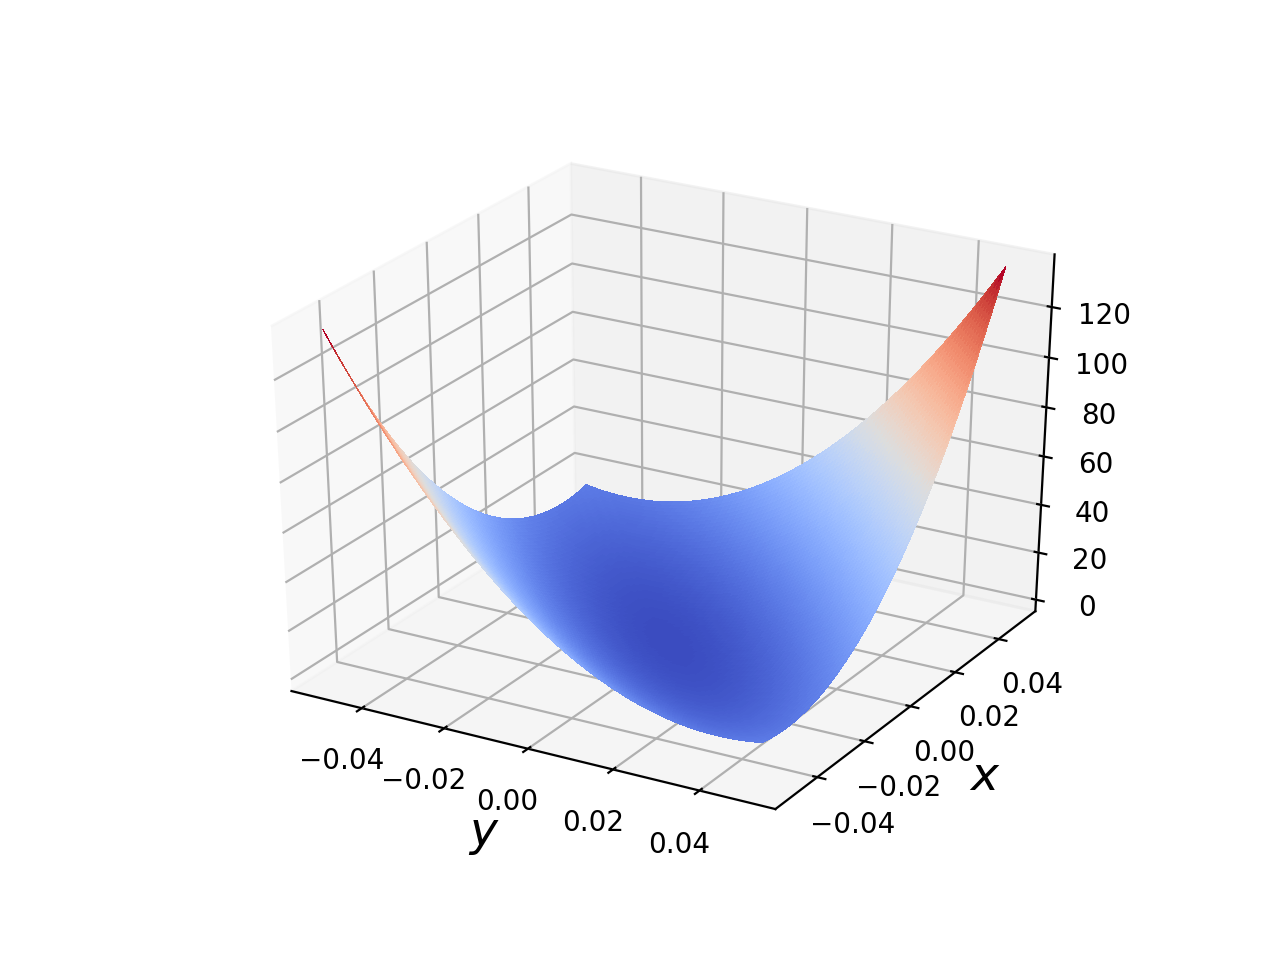
\includegraphics[width=\textwidth]{/home/hossein4527/MEGA/MEGAsync/Commit/University-Projects/MSc_Thesis/plots/Fig:(2d).png}
  			\caption{$Q_{total}$}
  			\label{fig:1.2.4}
  		\end{subfigure}
  		\caption{$\protect\rho =0.5$ و $\protect\sigma _{x}=\protect\sigma _{y}$}
  		\label{fig:1.2}	
  	\end{subfigure}
  	\begin{subfigure}[b]{\textwidth}
  		\renewcommand\thesubfigure{c}
  		\begin{subfigure}[b]{0.24\textwidth}
  			\renewcommand\thesubfigure{i}
  			\centering
  			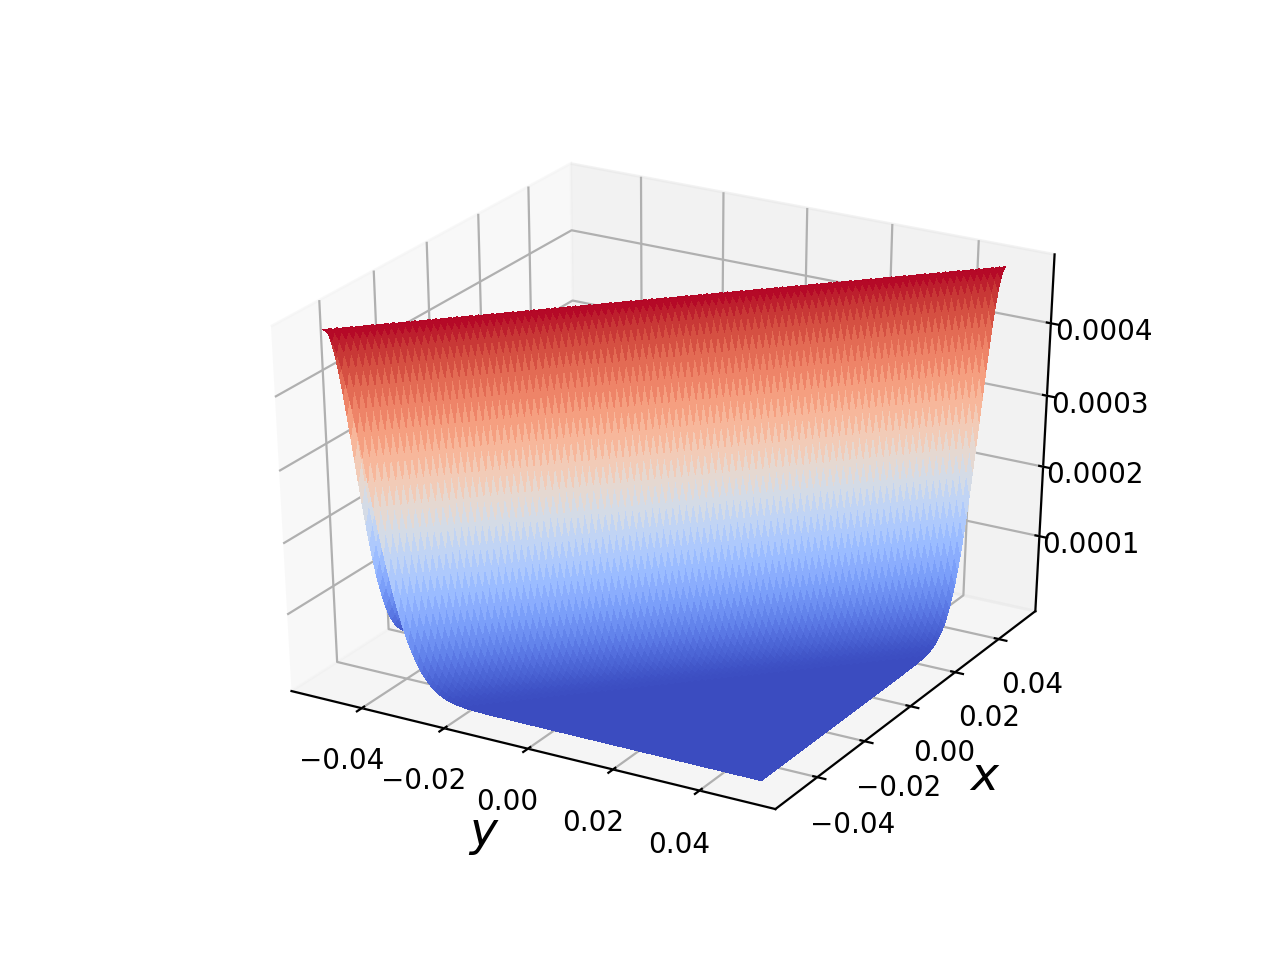
\includegraphics[width=\textwidth]{/home/hossein4527/MEGA/MEGAsync/Commit/University-Projects/MSc_Thesis/plots/Fig:(3a).png}
  			\caption{$Joint PDF$}
  			\label{fig:1.3.1}
  		\end{subfigure}
  		\hfill
  		\begin{subfigure}[b]{0.24\textwidth}
  			\renewcommand\thesubfigure{ii}
  			\centering
  			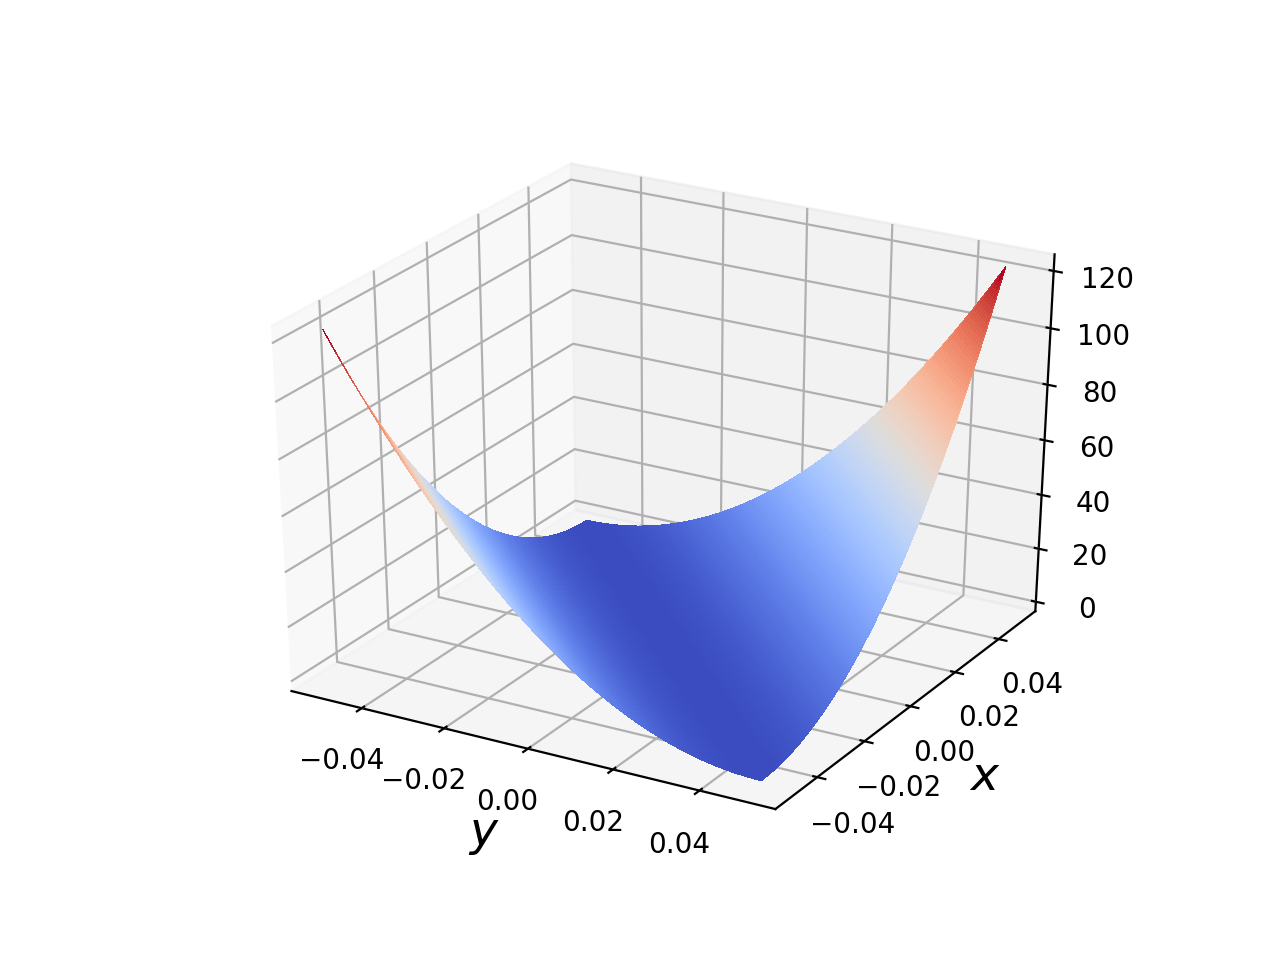
\includegraphics[width=\textwidth]{/home/hossein4527/MEGA/MEGAsync/Commit/University-Projects/MSc_Thesis/plots/Fig:(3b).png}
  			\caption{$Q_{x:y}$}
  			\label{fig:1.3.2}
  		\end{subfigure}
  		\hfill
  		\begin{subfigure}[b]{0.24\textwidth}
  			\renewcommand\thesubfigure{iii}
  			\centering
  			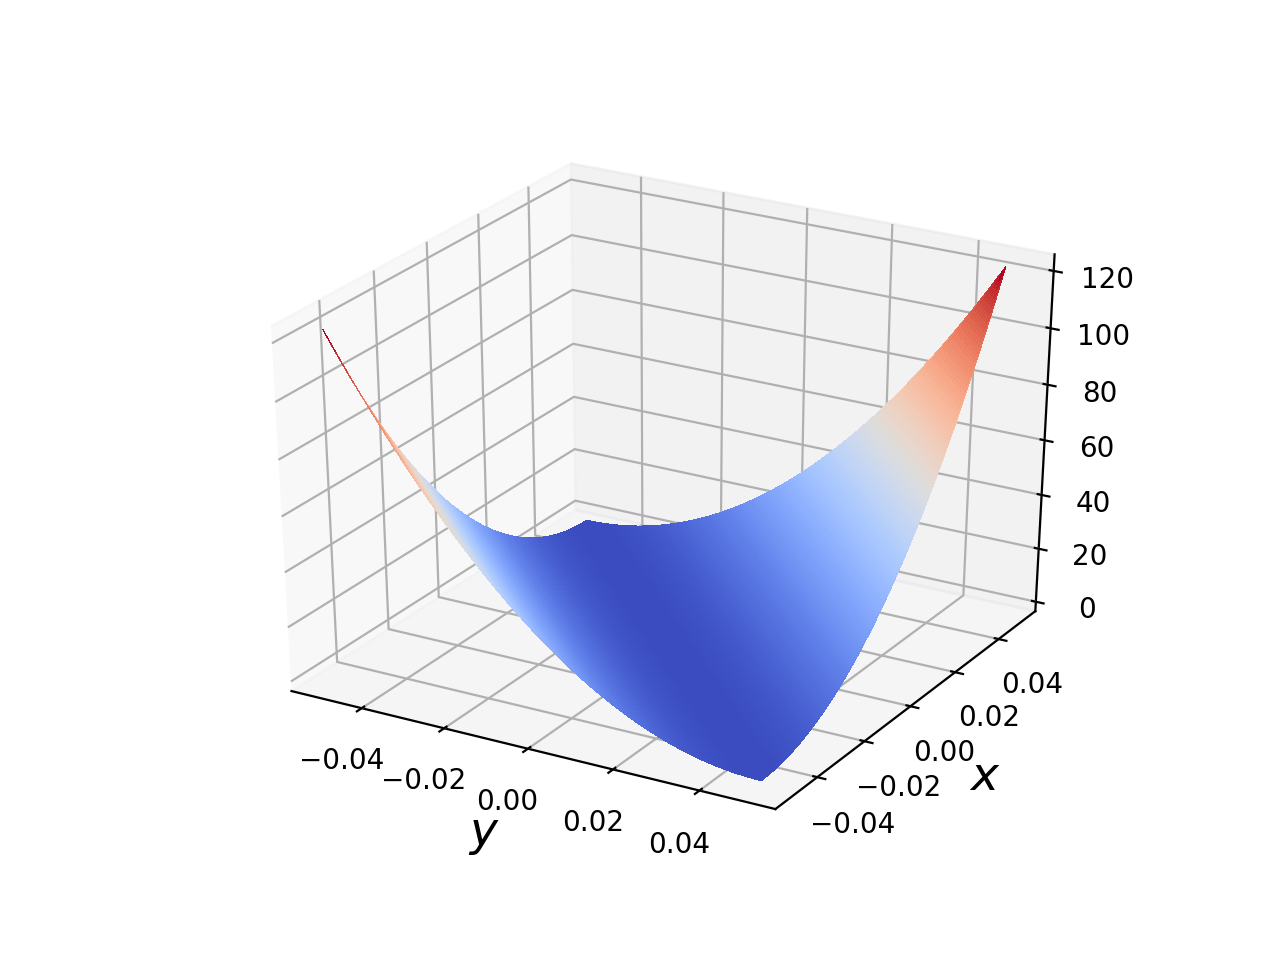
\includegraphics[width=\textwidth]{/home/hossein4527/MEGA/MEGAsync/Commit/University-Projects/MSc_Thesis/plots/Fig:(3c).png}
  			\caption{$Q_{y:x}$}
  			\label{fig:1.3.3}
  		\end{subfigure}
  		\hfill
  		\begin{subfigure}[b]{0.24\textwidth}
  			\renewcommand\thesubfigure{iv}
  			\centering
  			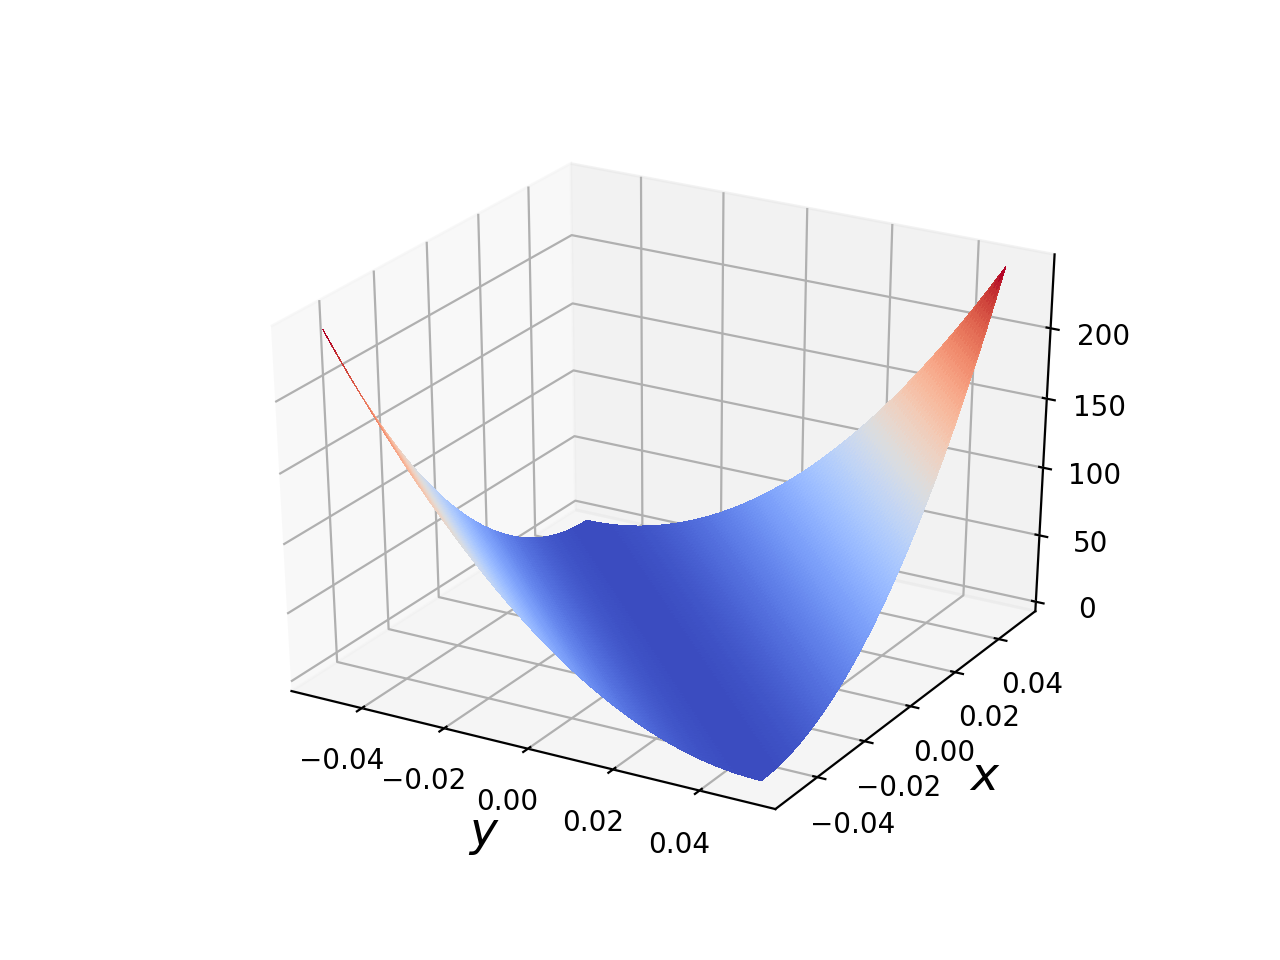
\includegraphics[width=\textwidth]{/home/hossein4527/MEGA/MEGAsync/Commit/University-Projects/MSc_Thesis/plots/Fig:(3d).png}
  			\caption{$Q_{total}$}
  			\label{fig:1.3.4}
  		\end{subfigure}
  		\caption{$\protect\rho =1$ و $\protect\sigma _{x}=\protect\sigma _{y}$}
  		\label{fig:1.3}
  	\end{subfigure}	
  	\caption{  		شکل سه بعدی تابع توزیع و پتانسیل های کوانتومی مربوطه رسم شده برای 
  		 $\protect\rho =0, 0.5, 1$ و  $\protect\sigma _{x}=%
  		\protect\sigma _{y}$.}
  	\label{fig:1t}
  \end{figure}
  
  \begin{figure}[tbp]
  	\centering
  	\begin{subfigure}[b]{\textwidth}
  		\renewcommand\thesubfigure{a}
  		\begin{subfigure}[b]{0.24\textwidth}
  			\renewcommand\thesubfigure{i}
  			\centering
  			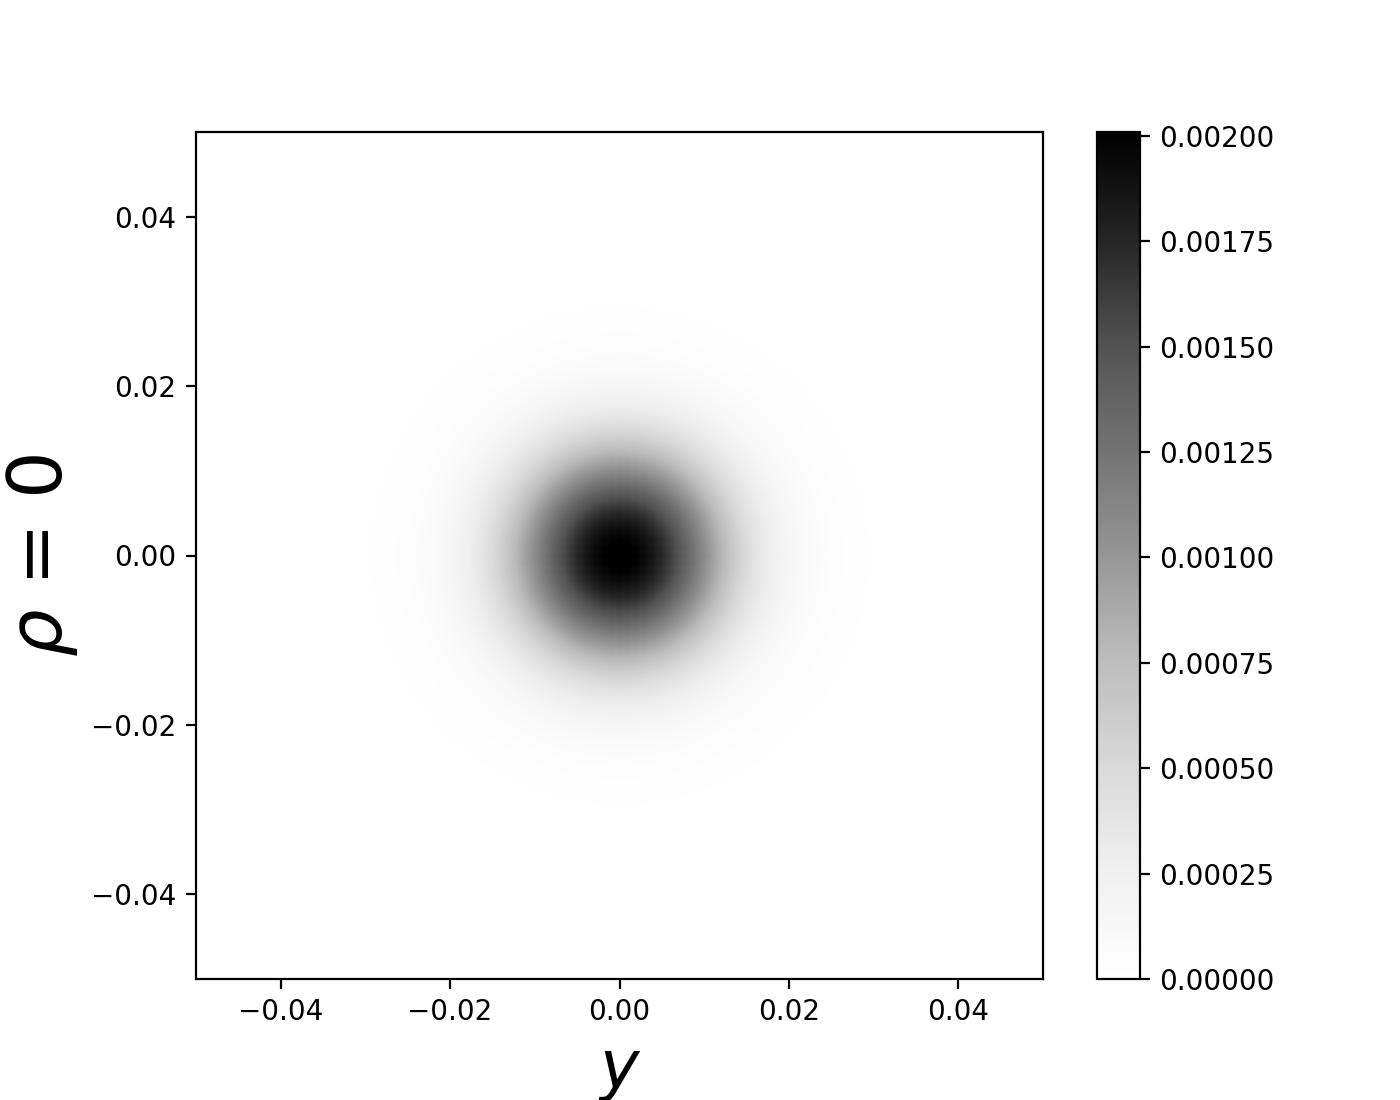
\includegraphics[width=\textwidth]{/home/hossein4527/MEGA/MEGAsync/Commit/University-Projects/MSc_Thesis/plots/Fig:(4a).png}
  			\caption{$Joint PDF$}
  			\label{fig:2.1.1}
  		\end{subfigure}
  		\hfill
  		\begin{subfigure}[b]{0.24\textwidth}
  			\renewcommand\thesubfigure{ii}
  			\centering
  			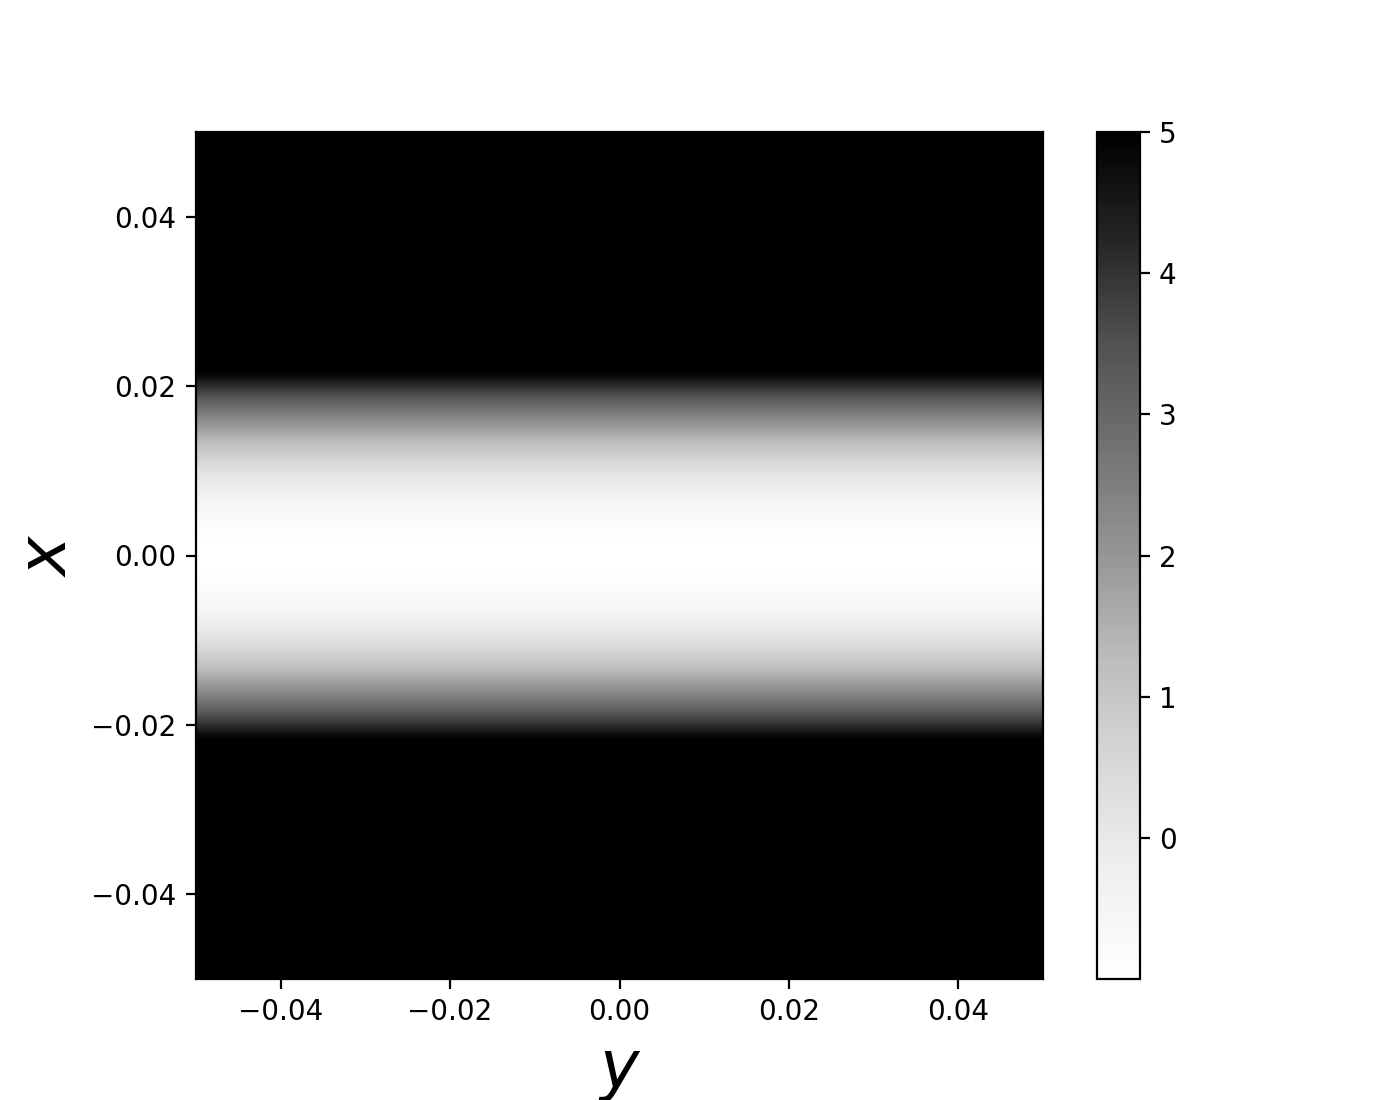
\includegraphics[width=\textwidth]{/home/hossein4527/MEGA/MEGAsync/Commit/University-Projects/MSc_Thesis/plots/Fig:(4b).png}
  			\caption{$Q_{x:y}$}
  			\label{fig:2.1.2}
  		\end{subfigure}
  		\hfill
  		\begin{subfigure}[b]{0.24\textwidth}
  			\renewcommand\thesubfigure{iii}
  			\centering
  			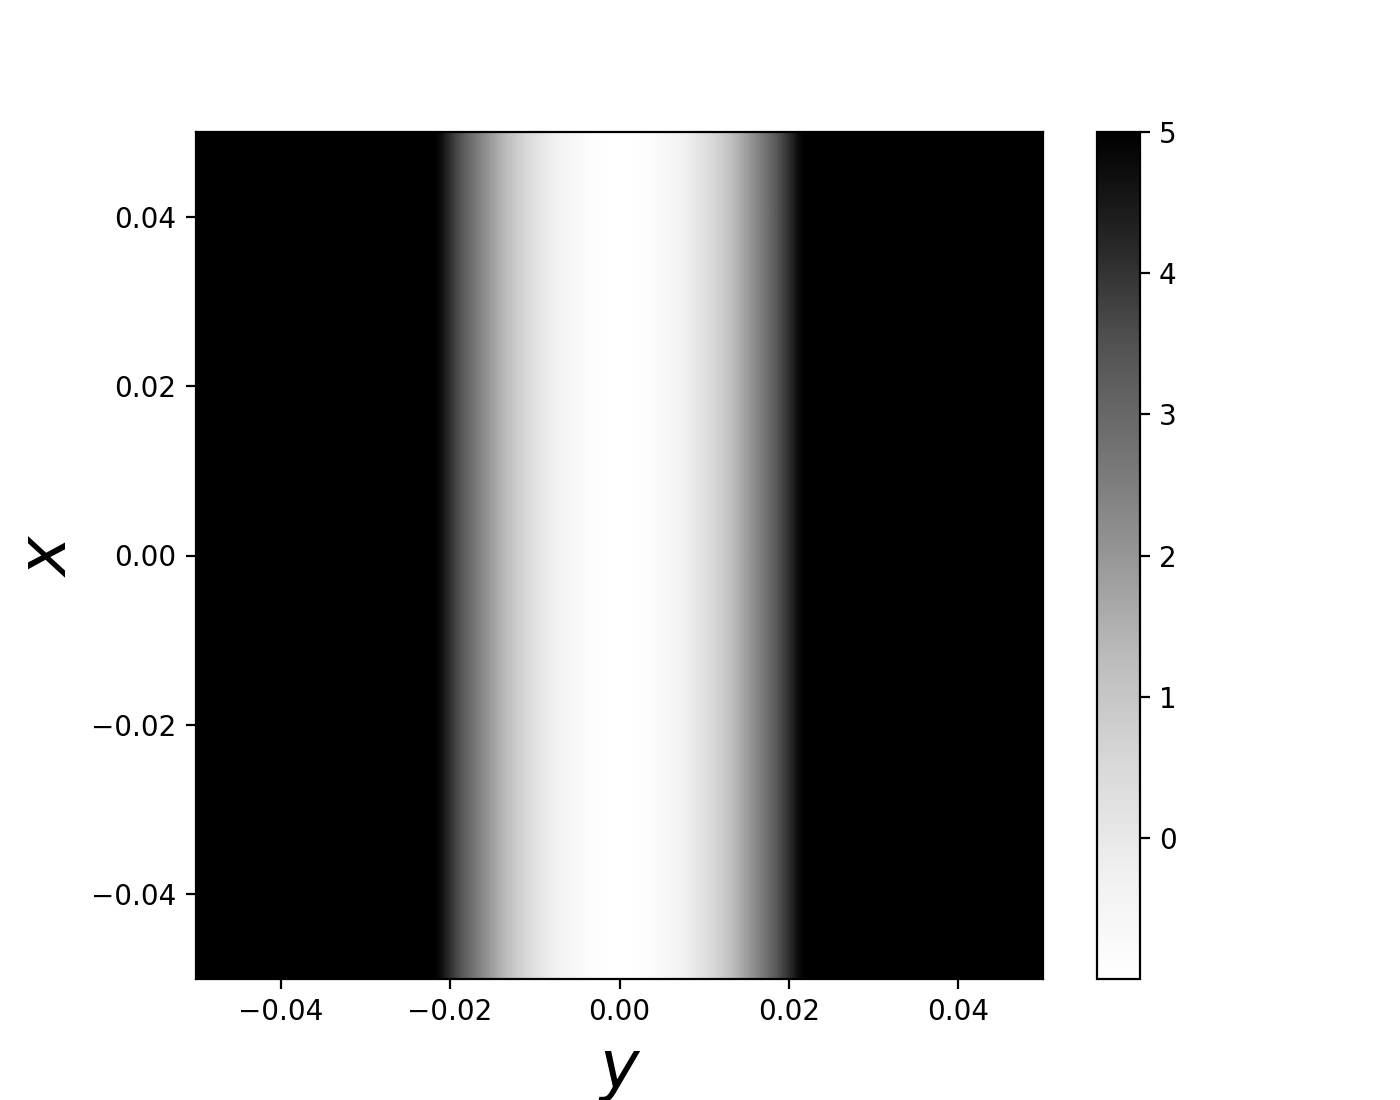
\includegraphics[width=\textwidth]{/home/hossein4527/MEGA/MEGAsync/Commit/University-Projects/MSc_Thesis/plots/Fig:(4c).png}
  			\caption{$Q_{y:x}$}
  			\label{fig:2.1.3}
  		\end{subfigure}
  		\hfill
  		\begin{subfigure}[b]{0.24\textwidth}
  			\renewcommand\thesubfigure{iv}
  			\centering
  			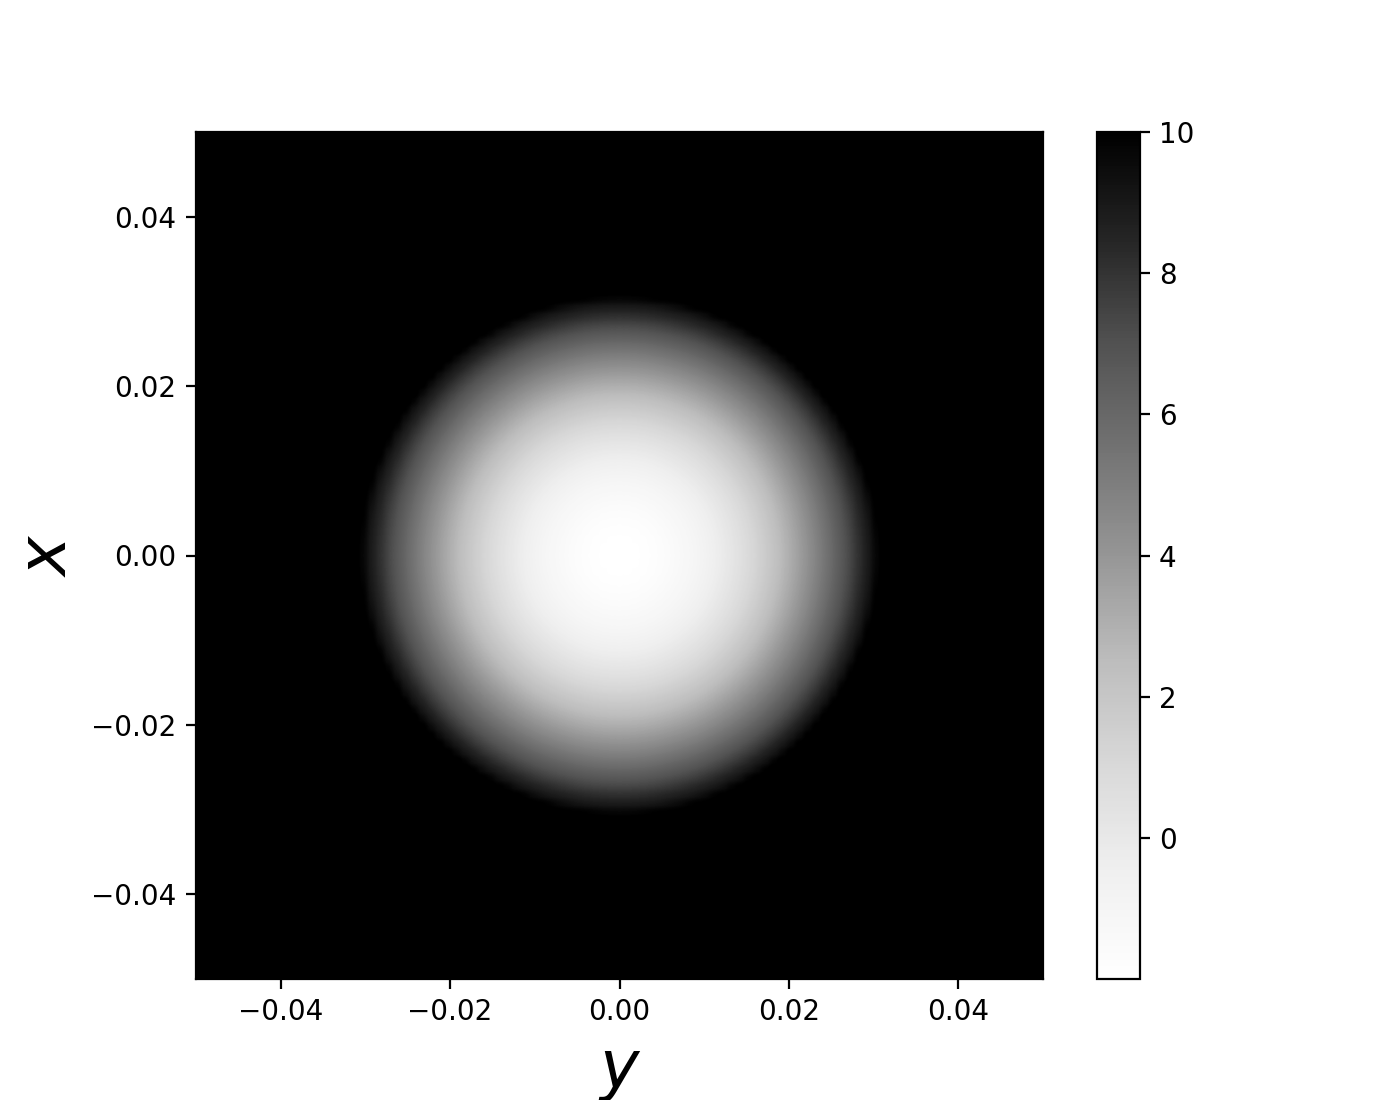
\includegraphics[width=\textwidth]{/home/hossein4527/MEGA/MEGAsync/Commit/University-Projects/MSc_Thesis/plots/Fig:(4d).png}
  			\caption{$Q_{total}$}
  			\label{fig:2.1.4}
  		\end{subfigure}
  		\caption{$\protect\rho =0$ و $\protect\sigma _{x}=\protect\sigma _{y}$}
  		\label{fig:2.1}
  	\end{subfigure}
  	\begin{subfigure}[b]{\textwidth}
  		\renewcommand\thesubfigure{b}
  		\begin{subfigure}[b]{0.24\textwidth}
  			\renewcommand\thesubfigure{i}
  			\centering
  			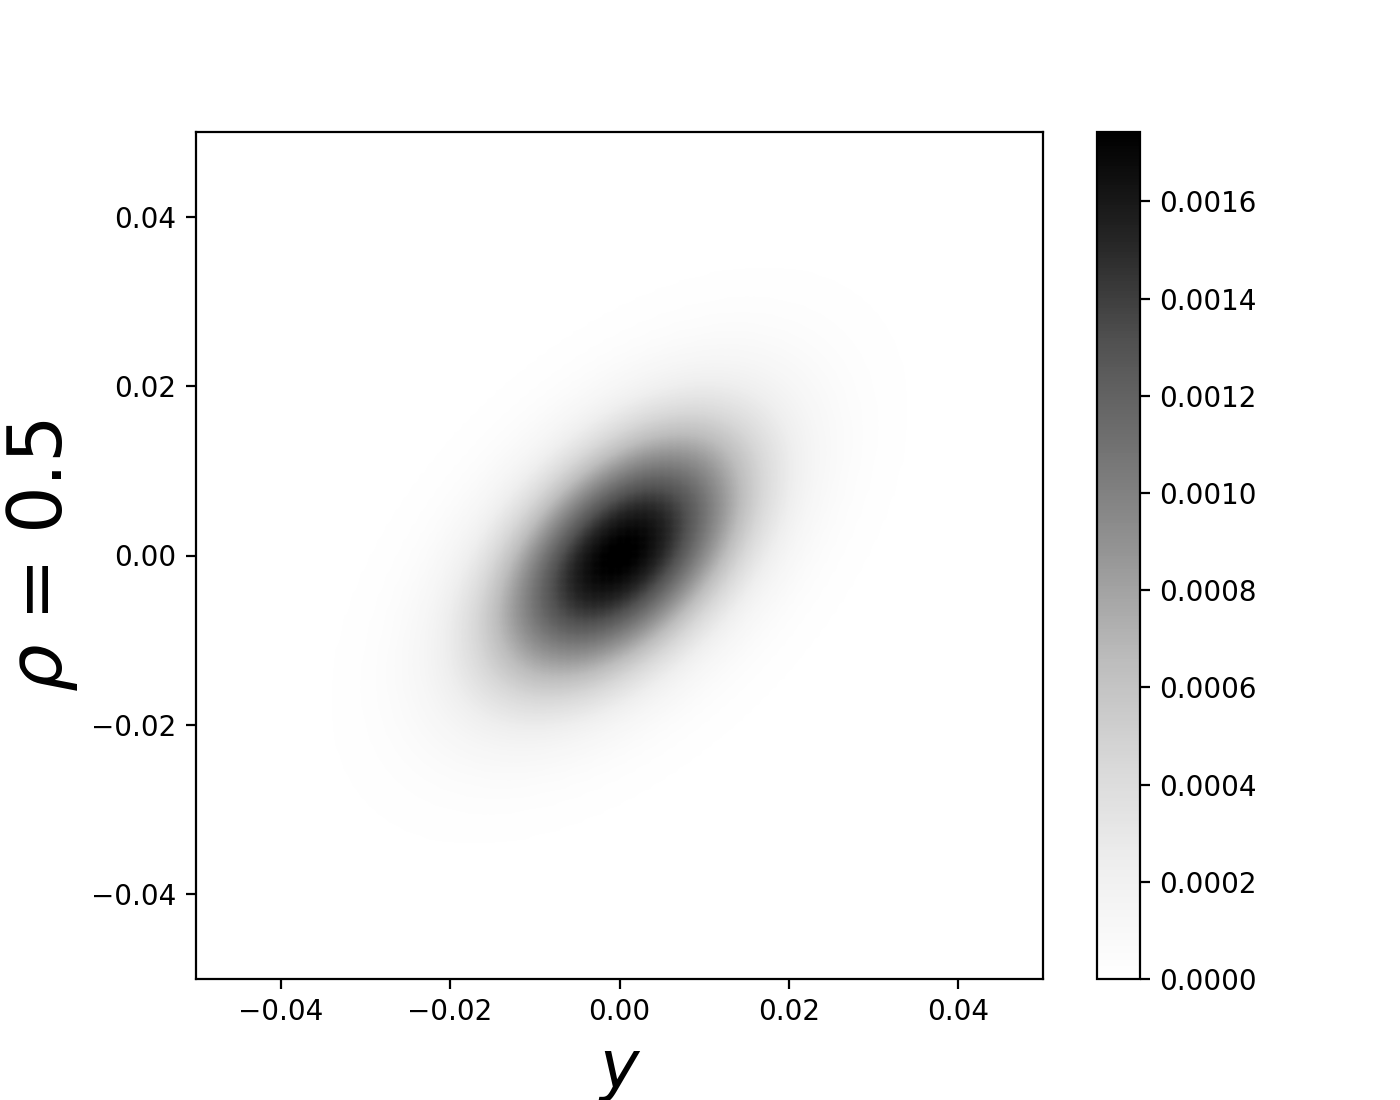
\includegraphics[width=\textwidth]{/home/hossein4527/MEGA/MEGAsync/Commit/University-Projects/MSc_Thesis/plots/Fig:(5a).png}
  			\caption{$Joint PDF$}
  			\label{fig:2.2.1}
  		\end{subfigure}
  		\hfill
  		\begin{subfigure}[b]{0.24\textwidth}
  			\renewcommand\thesubfigure{ii}
  			\centering
  			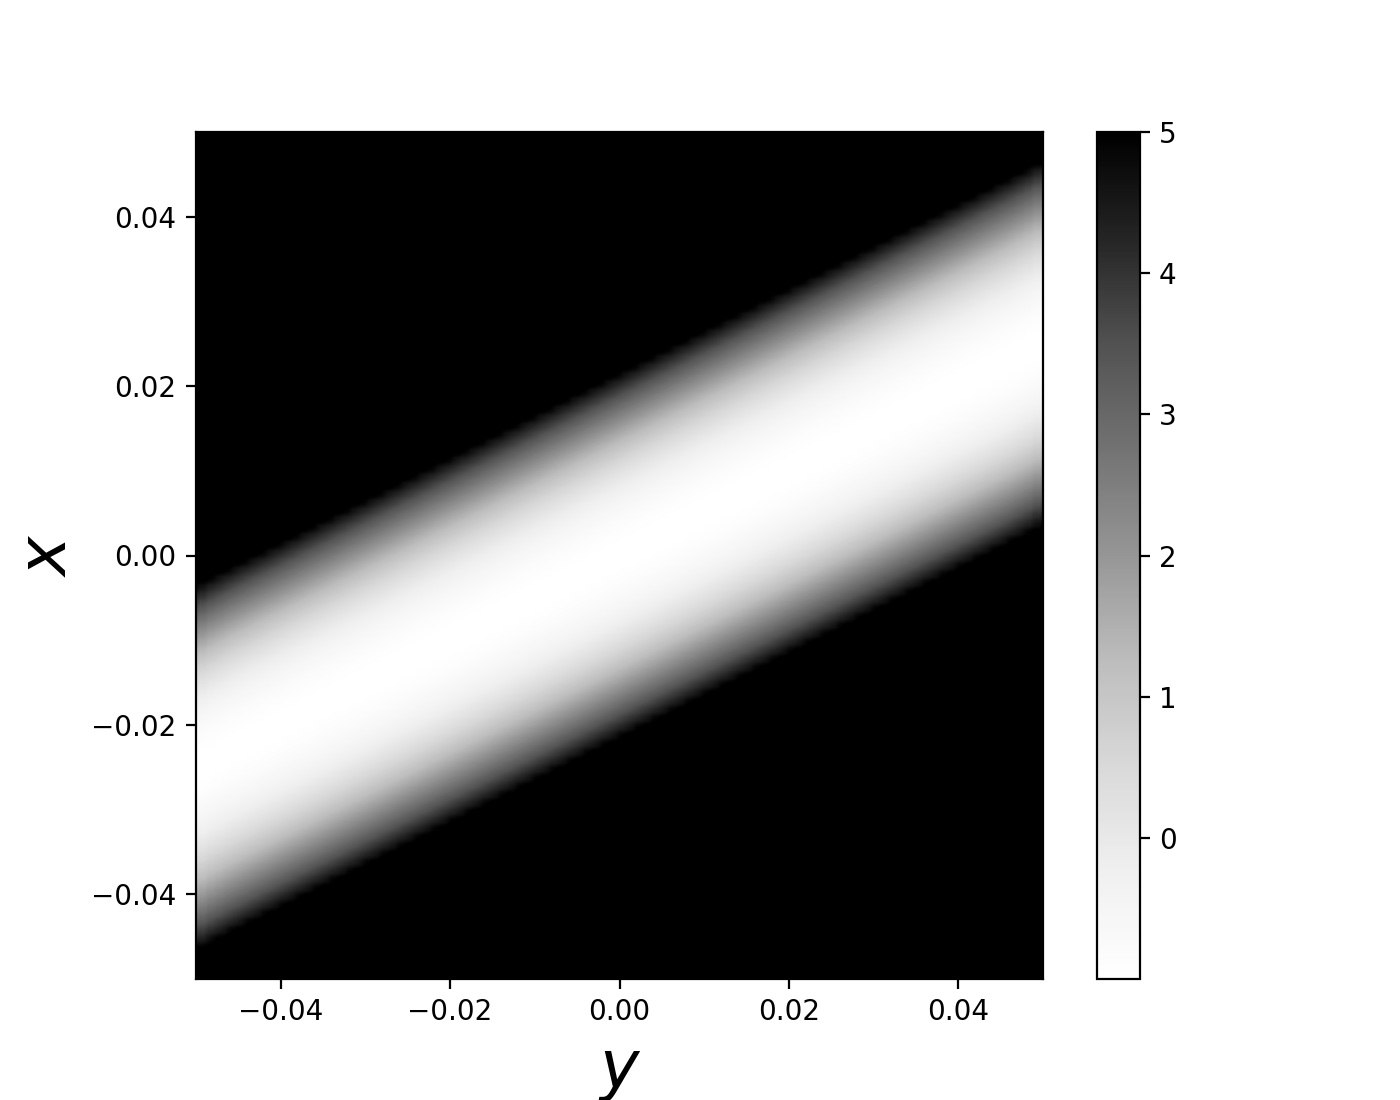
\includegraphics[width=\textwidth]{/home/hossein4527/MEGA/MEGAsync/Commit/University-Projects/MSc_Thesis/plots/Fig:(5b).png}
  			\caption{$Q_{x:y}$}
  			\label{fig:2.2.2}
  		\end{subfigure}
  		\hfill
  		\begin{subfigure}[b]{0.24\textwidth}
  			\renewcommand\thesubfigure{iii}
  			\centering
  			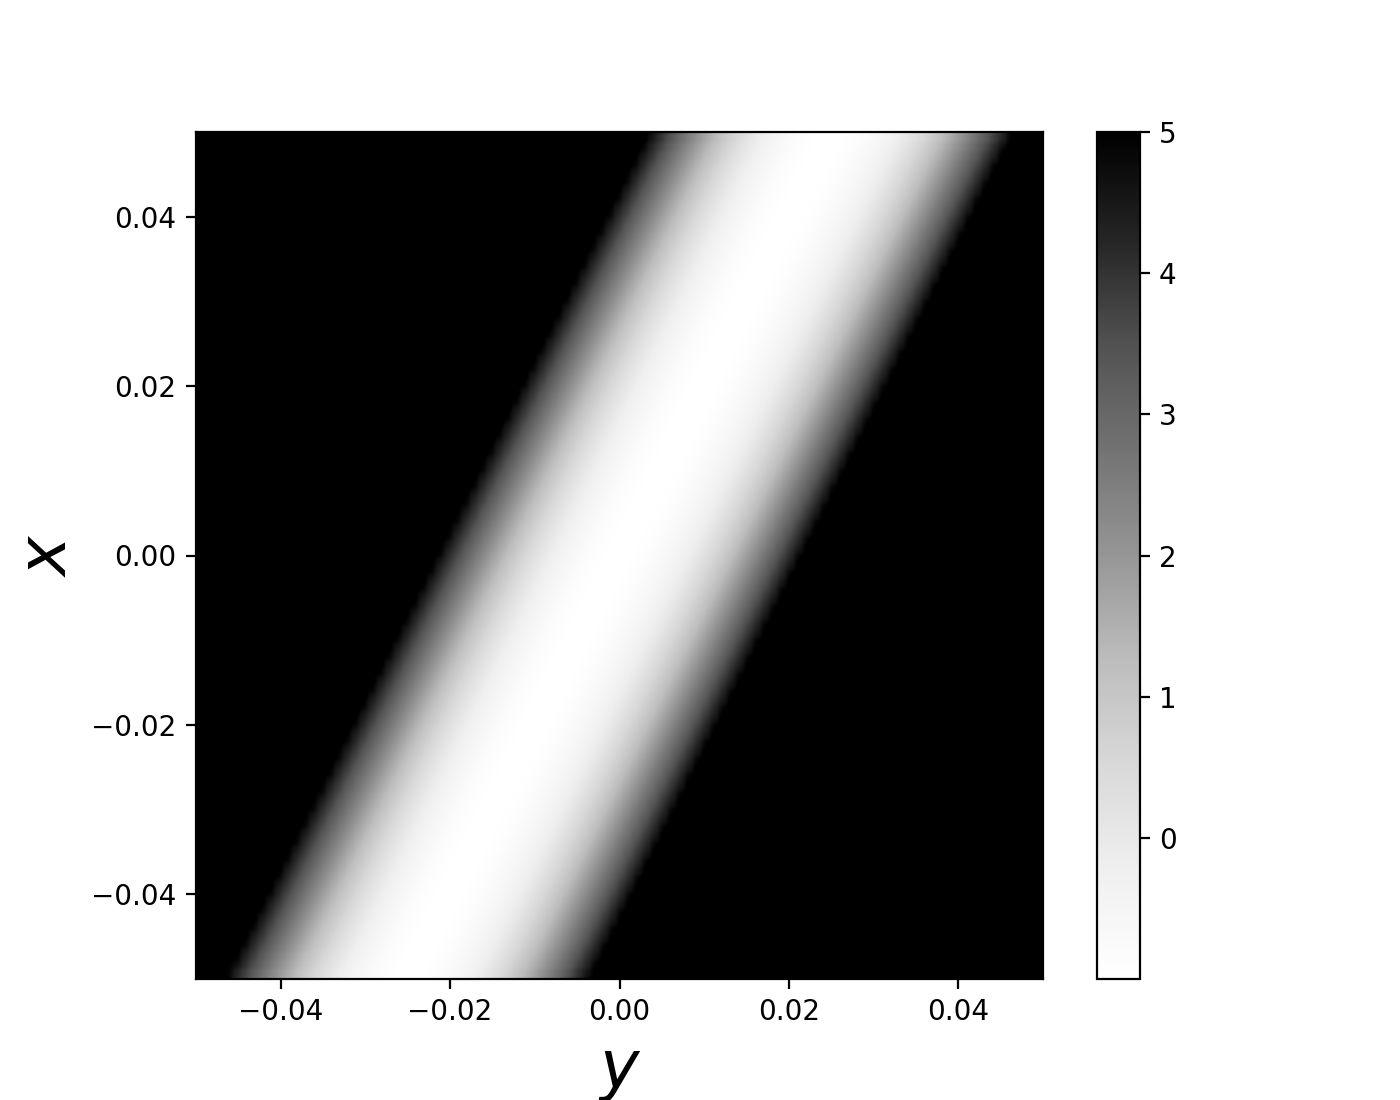
\includegraphics[width=\textwidth]{/home/hossein4527/MEGA/MEGAsync/Commit/University-Projects/MSc_Thesis/plots/Fig:(5c).png}
  			\caption{$Q_{y:x}$}
  			\label{fig:2.2.3}
  		\end{subfigure}
  		\hfill
  		\begin{subfigure}[b]{0.24\textwidth}
  			\renewcommand\thesubfigure{iv}
  			\centering
  			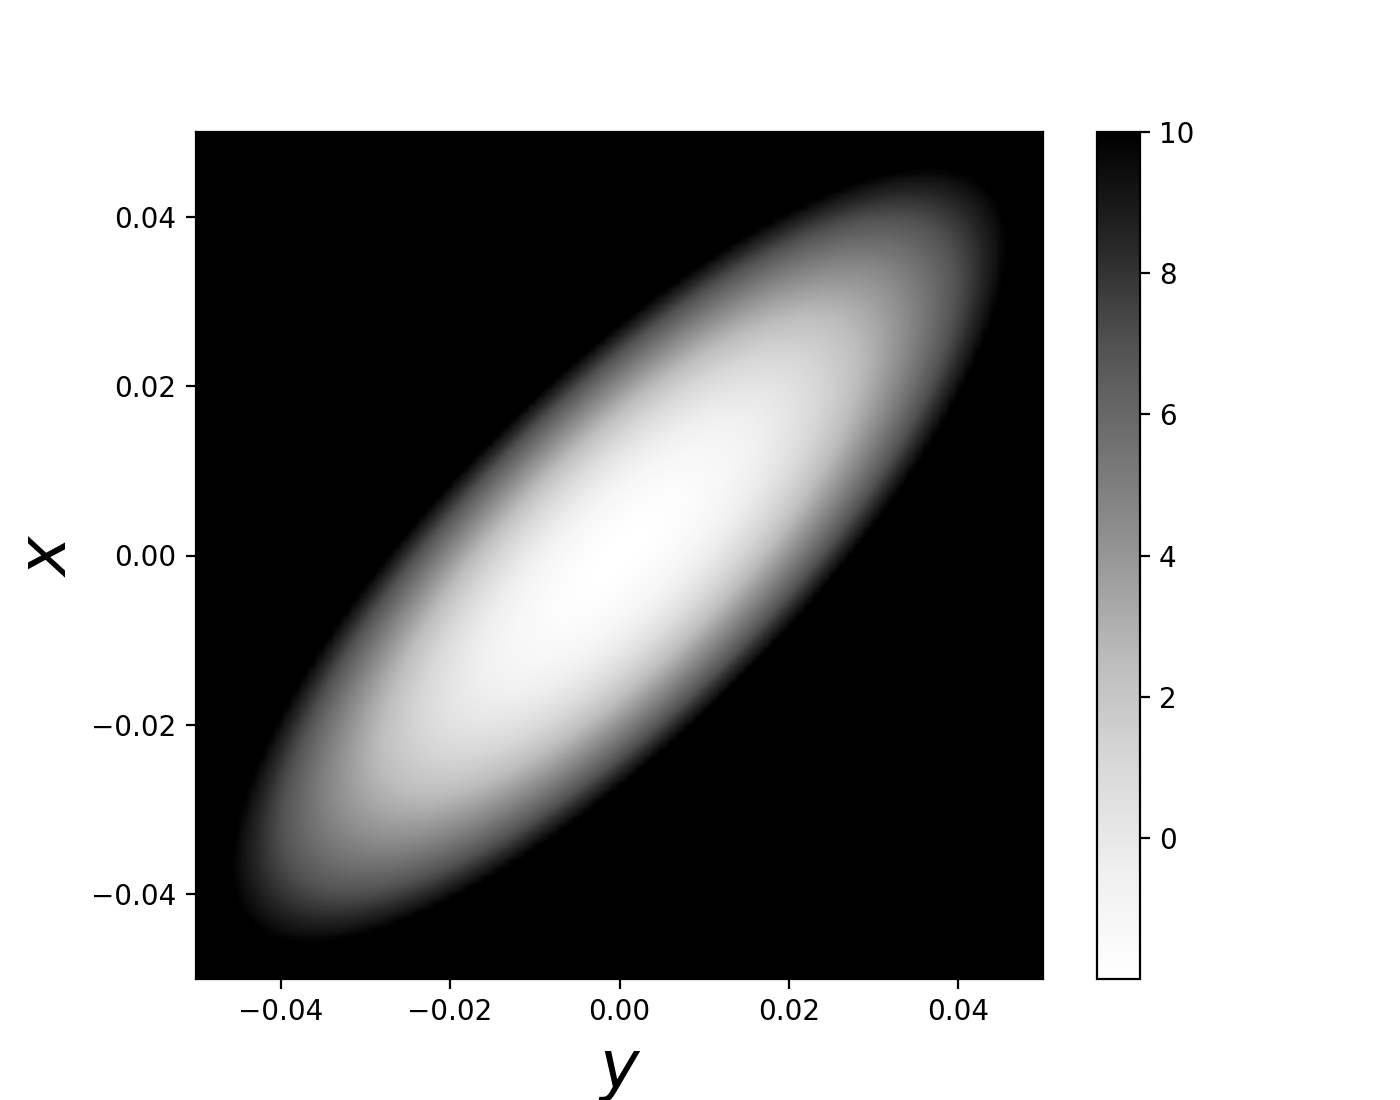
\includegraphics[width=\textwidth]{/home/hossein4527/MEGA/MEGAsync/Commit/University-Projects/MSc_Thesis/plots/Fig:(5d).png}
  			\caption{$Q_{total}$}
  			\label{fig:2.2.4}
  		\end{subfigure}
  		\caption{$\protect\rho =0.5$ و $\protect\sigma _{x}=\protect\sigma _{y}$}
  		\label{fig:2.2}
  	\end{subfigure}
  	\begin{subfigure}[b]{\textwidth}
  		\renewcommand\thesubfigure{c}
  		\begin{subfigure}[b]{0.24\textwidth}
  			\renewcommand\thesubfigure{i}
  			\centering
  			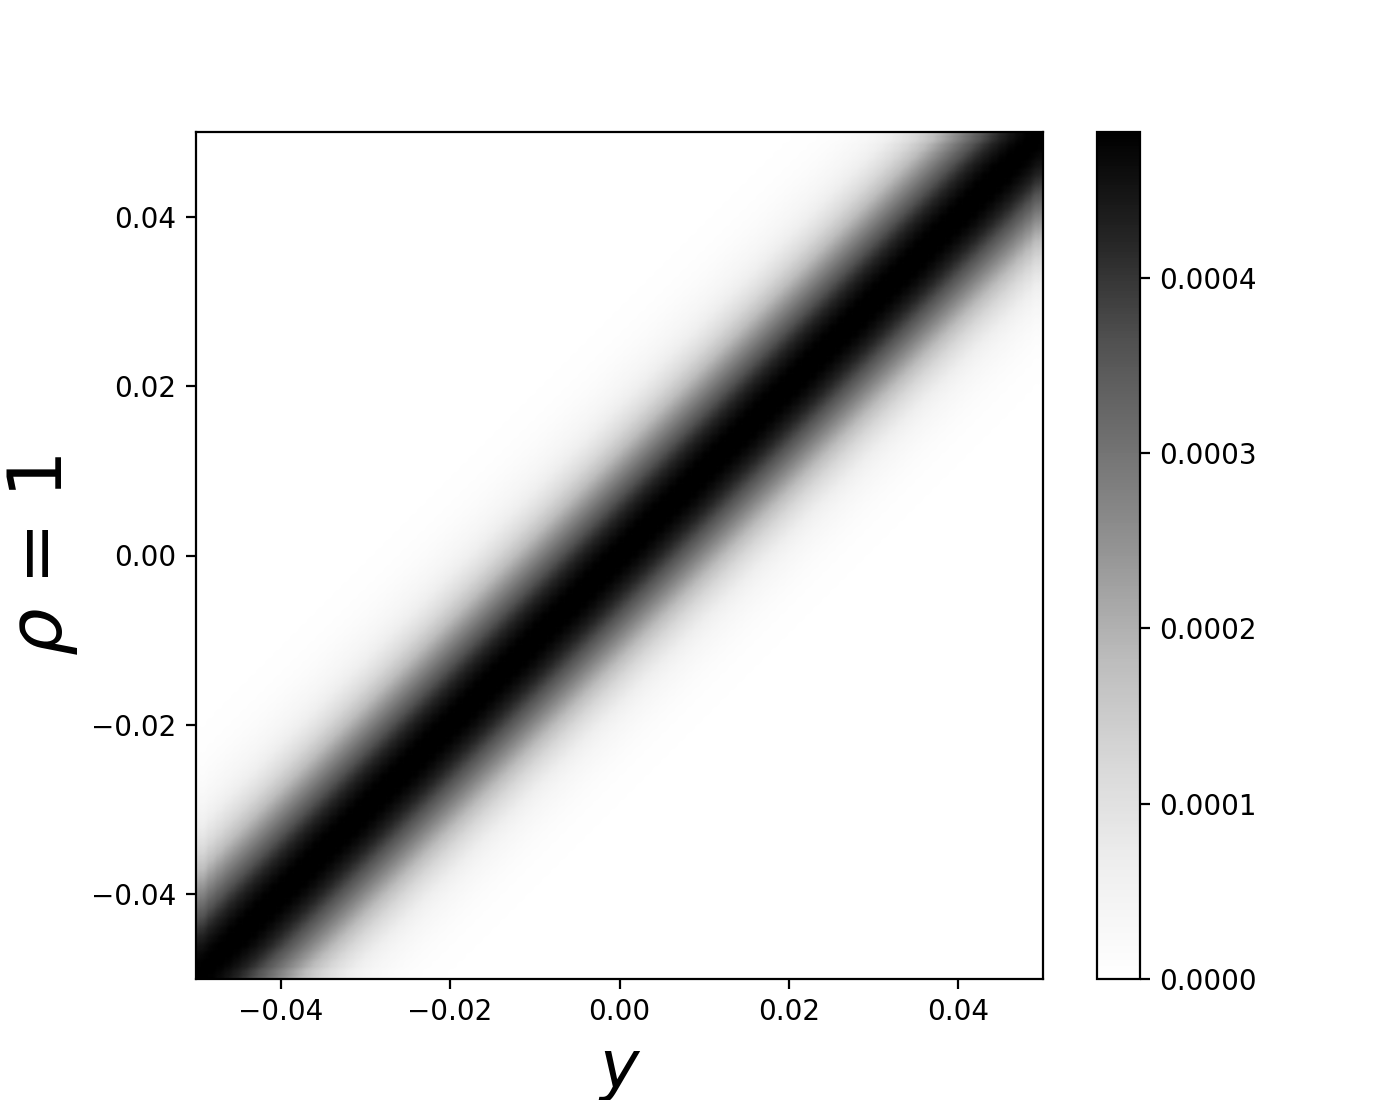
\includegraphics[width=\textwidth]{/home/hossein4527/MEGA/MEGAsync/Commit/University-Projects/MSc_Thesis/plots/Fig:(6a).png}
  			\caption{$Joint PDF$}
  			\label{fig:2.3.1}
  		\end{subfigure}
  		\hfill
  		\begin{subfigure}[b]{0.24\textwidth}
  			\renewcommand\thesubfigure{ii}
  			\centering
  			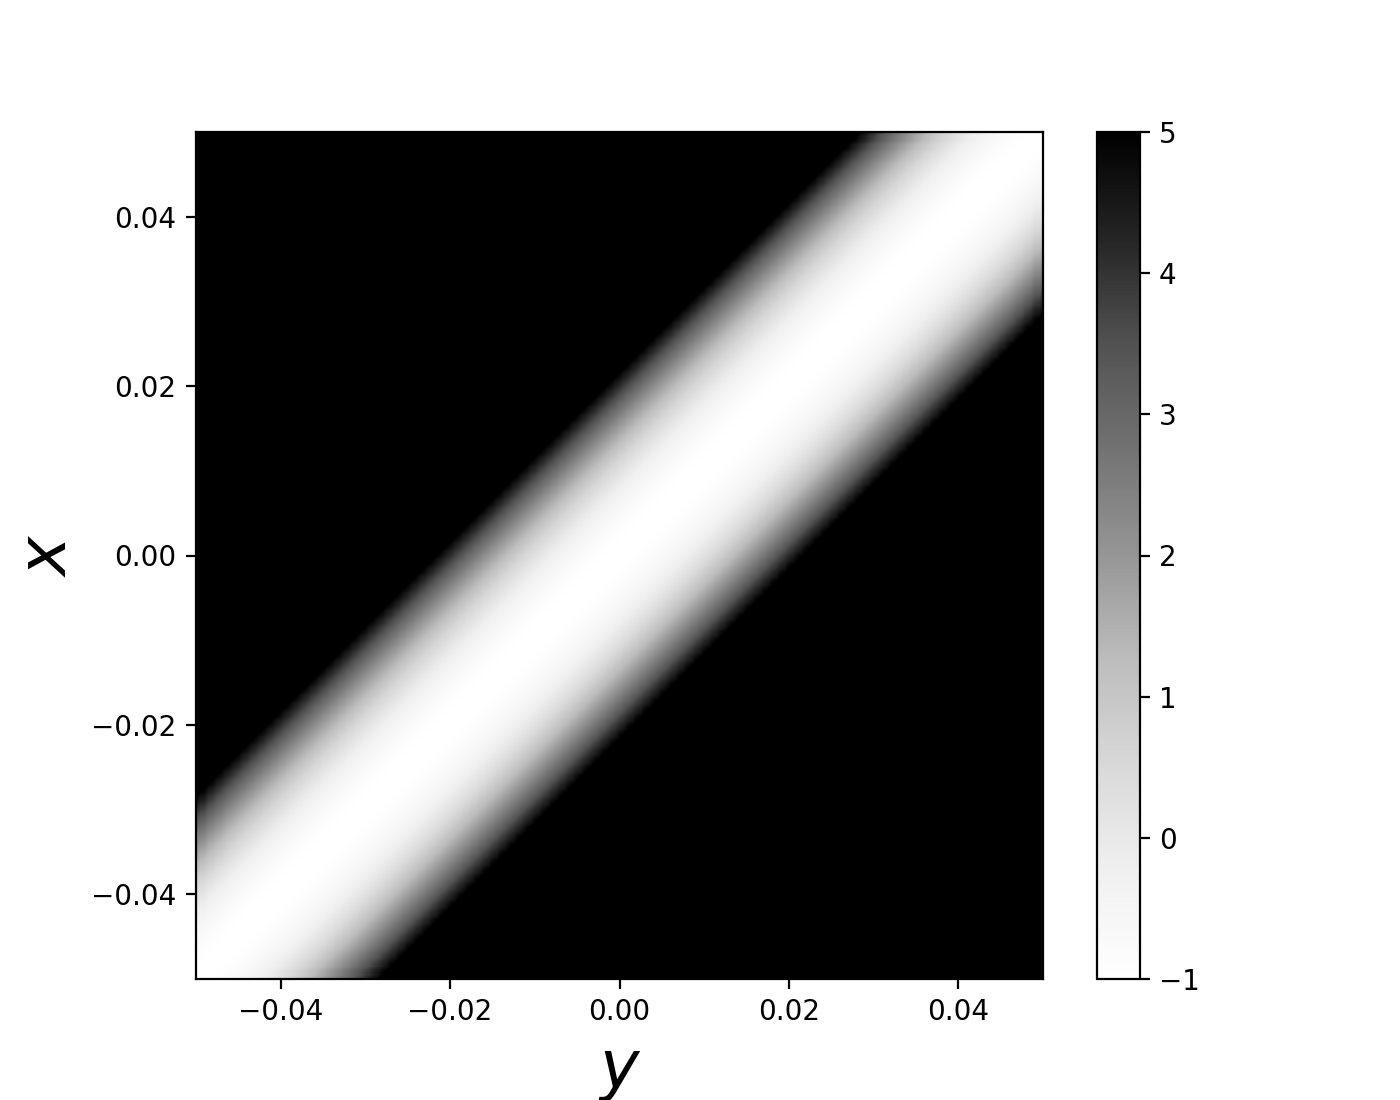
\includegraphics[width=\textwidth]{/home/hossein4527/MEGA/MEGAsync/Commit/University-Projects/MSc_Thesis/plots/Fig:(6b).png}
  			\caption{$Q_{x:y}$}
  			\label{fig:2.3.2}
  		\end{subfigure}
  		\hfill
  		\begin{subfigure}[b]{0.24\textwidth}
  			\renewcommand\thesubfigure{iii}
  			\centering
  			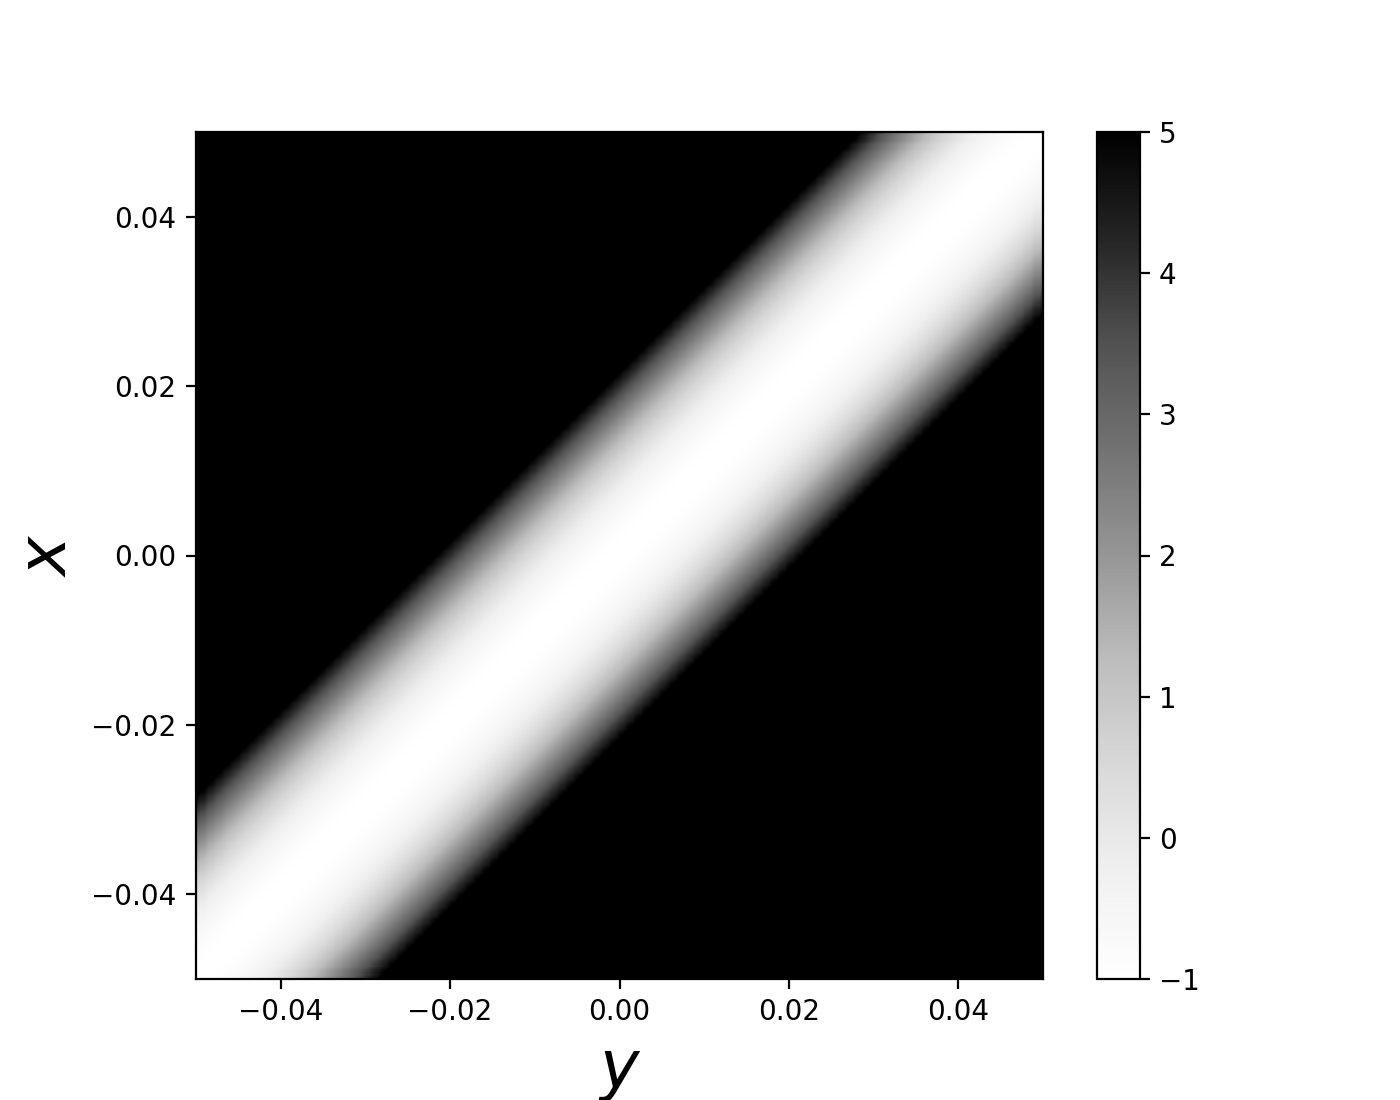
\includegraphics[width=\textwidth]{/home/hossein4527/MEGA/MEGAsync/Commit/University-Projects/MSc_Thesis/plots/Fig:(6c).png}
  			\caption{$Q_{y:x}$}
  			\label{fig:2.3.3}
  		\end{subfigure}
  		\hfill
  		\begin{subfigure}[b]{0.24\textwidth}
  			\renewcommand\thesubfigure{iv}
  			\centering
  			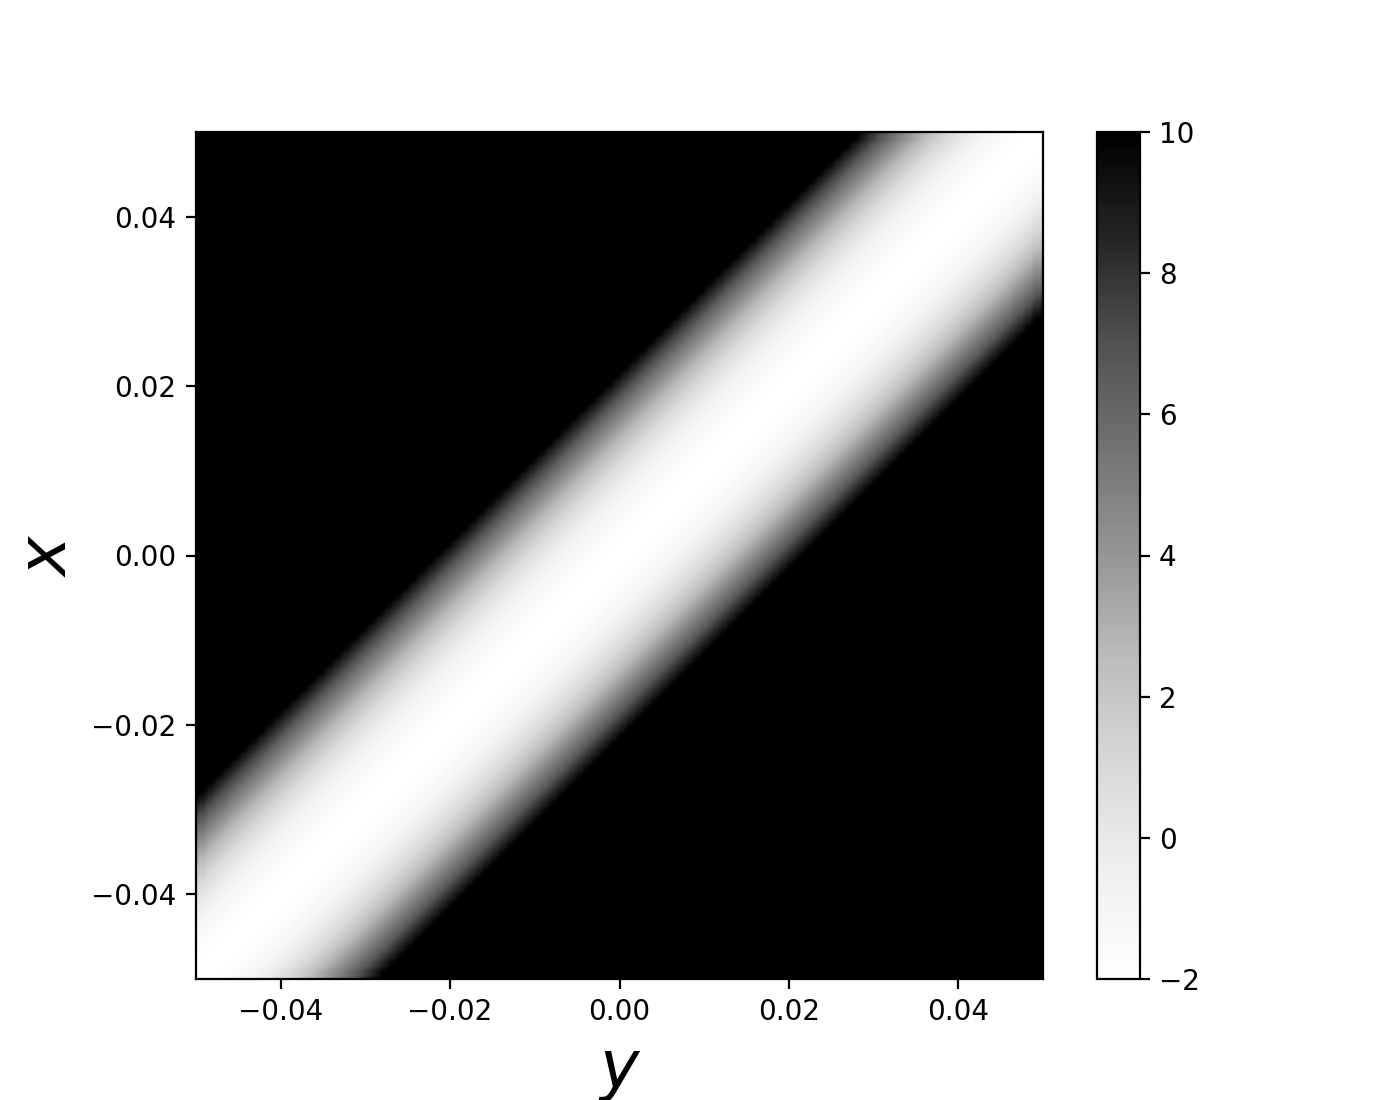
\includegraphics[width=\textwidth]{/home/hossein4527/MEGA/MEGAsync/Commit/University-Projects/MSc_Thesis/plots/Fig:(6d).png}
  			\caption{$Q_{total}$}
  			\label{fig:2.3.4}
  		\end{subfigure}		
  		\caption{$\protect\rho =1$ و $\protect\sigma _{x}=\protect\sigma _{y}$}
  		\label{fig:2.3}
  	\end{subfigure}
  	\caption{شکل سه بعدی گرمایی رسم شده برای تابع توزیع و پتانسیل های مربوطه برای
  		 $\protect\rho =0,0.5,1$ و $\protect\sigma _{x}=\protect\sigma %
  		_{y}$.}
  	\label{fig:2t}
  \end{figure}
در شکل 
\ref{fig:1.1.1}
تابع توزیع مشترک تحت عنوان تابعی از 
$r_1$
و
$r_2$
برای ضریب همبستگی، 
$\rho=0$
رسم شده است. این تابع نسبت به محور های مختصات 
$r_1$
و
$r_2$
متقارن است. در شکل های 
\ref{fig:1.1.2}
و
\ref{fig:1.1.3}
پتانسیل های کوانتومی شرطی 
$Q_{r_1:r_2}$
و
$Q_{r_2:r_1}$
به ترتیب برای همان مقادیر 
$r_1$
و
$r_2$
شکل
\ref{fig:1.1.1}
رسم شده اند. همانطور که در شکل پیداست، این پتانسیل ها برای مقادیر 
$\rho=0$
و 
$\sigma_1=\sigma_2$
بر یکدیگر عمود هستند. عمود بودن این دو پتانسیل با وضوح بهتری در شکل 
\ref{fig:2.1}
مشخص است. پتانسیل کوانتومی کل رسم شده در شکل سه بعدی
\ref{fig:1.1.4}
و شکل نقشه حرارتی 
\ref{fig:2.1.4}
کاملن متقارن و برش های موازی محور های مختصات آن شبیه دایره است. دایره  بودن این پتانسیل برای شرایط (a)
$\rho=0$
و 
$\sigma_1=\sigma_2$
بدون خطا و قطعی است.

در قسمت های (b) و (c) دو شکل زیر مقادیر غیر صفر ضریب همبستگی بین دو بازار بررسی شده اند.
مطابق شکل های
\ref{fig:1t}
و 
\ref{fig:2t}
با زیاد شدن 
$\rho$
تابع توزیع مشترک در راستای نیمساز محور های مختصات کشیده شده و همین اتفاق مسبب چرخش پتانسیل های کوانتومی شرطی شده است. این پتانسیل ها در خلاف جهت یکدیگر شروع به چرخش میکنند و متناسب با میزان افزایش ضریب همبستگی 
$\rho$
زاویه ای با محور های مختصات می سازند. چرخش این پتانسیل های کوانتومی شرطی سبب هیچ چرخشی در پتانسیل کوانتومی کل نمی شود و تنها باعث کشیده شدن این پتانسیل در راستای نیمساز محور های مختصات خواهد شد. این مساله به وضوح در شکل های
\ref*{fig:2.2.4}
و 
\ref*{fig:2.3.4}
قابل مشاهده است.
پس در این قسمت فهمیدیم که برای بازار های با واریانس سود یکسان، 
$\sigma_1=\sigma_2$
 با افزایش میزان ضریب همبستگی بین دو بازار، 
  $\rho$
   پتانسیل های کوانتومی شرطی 
   $Q_{r_1:r_2}$
   و
   $Q_{r_2:r_1}$
   شروع به چرخش به ترتیب در جهت و خلاف عقربه های ساعت کرده و پتانسیل کوانتومی کل 
   $Q$
   در راستای نیمساز محورهای مختصات کشیده تر می شود. 
   
\subsection{
	بررسی متغیر 
	$\rho$
	برای بازارهای با واریانس غیر  یکسان،
	$\sigma_1 \neq \sigma_2$
}
برای مقادیر مختلفی از ضریب همبستگی 
$\rho$
و بازار های با واریانس سود متفاوت،
$\sigma_1 \neq \sigma_2$
توابع توزیع مشترک و پتانسیل های مربوطه در شکل 
\ref{fig:3t}
رسم شده اند.  با توجه به شکل، در قسمت i(a) تابع توزیع مشترک برای دو بازار بدون همبستگی و با شرایط واریانس
$\sigma_1 =2\sigma_2$
آورده شده است. با مقایسه این شکل و شکل 

\ref{fig:2.1.1}
که همین تابع توزیع برای واریانس های برابر است، می توان نتیجه گرفت که اختلاف واریانس باعث کشیدگی تابع توزیع مشترک به سمت مختصات بازار با واریانس بیشتر می شود. این خاصیت به سادگی در ویژگی های توابع توزیع قابل مشاهده است و نکته ی جدیدی را به دانسته های ما اضافه نمی کند. لیکن در نتیجه ی این کشیدگی تابع توزیع تفاوت هایی در پتانسیل های کوانتومی مشترک نسبت به حالت قبلی،
$\sigma_1 =\sigma_2$
مشاهده می شود. پتانسیل کوانتومی شرطی محاسبه شده برای داده های با واریانس بیشتر عریض تر از پتانسیل دیگری است و به همین دلیل تقارن موجود در پتانسیل کوانتومی کل بر خلاف حالت قبلی شکسته می شود. با مشاهده پتانسیل کوانتومی کل در شکل
\ref{fig:3.1.4}
می توان نتیجه گرفت که برای بازار های با ضریب همبستگی صفر، پتانسیل کوانتومی تنها و تنها زمانی متقارن است که بازار ها دارای وارینس برابر باشند و این تقارن شکسته می شود زمانی که بین واریانس های آن دو اختلاف باشد و پتانسیل کل به سمت مختصات بازار با وارینس بیشتر کشیده می شود.
در قسمت های (b) و (c)  شکل
\ref*{fig:3t}
ضرایب همبستگی 
$0.5$
و
$1$
انتخاب شده است و توابع مربوطه رسم شده اند. همانطور که در شکل پیداست، پتانسیل های کوانتومی شرطی زوایای متفاوتی نسبت به حالت 
$\sigma_1 =\sigma_2$
انتخاب کرده اند و پتانسیل بازاری با واریانس بیشتر زاویه ی بزرگ تری را نسبت به دیگری طی کرده است. در نتیجه ی این چرخش های متفاوت، پتانسیل کوانتومی کل که حاصل مجموع این دو پتانسیل کوانتومی شرطی است، دیگر نسبت به محور های مختصات تقارن ندارد و نسبت به محوری متفاوت با نیمساز محورهای مختصات کشیده شده است. این واقعیت به خوبی در شکل های 
\ref{fig:3.2.4}
و 
\ref{fig:3.3.4}
قابل مشاهده است. مطابق با این دو شکل، پتانسیل کوانتومی کل به سمت مختصات بازار با واریانس بیشتر کشیده تر می شود و فضای فاز سود و زیان بازار کم واریانس تر را محدود تر می کند. این واقعه با دانسته های ما از رفتار دو بازار کنار یکدیگر به خوبی مطابقت دارد. در هر دو بازار همبسته، اجازه ی سود و زیان در بازاری بیشتر خواهد بود که در مرحله ی اول واریانس بزرگتری داشته باشد. بازاری با واریانس محدود و کم، کم ریسک تر و به طبع آن کم بازده تر خواهد بود. 

 \begin{figure}[tbp]
	\centering
	\begin{subfigure}[b]{\textwidth}
		\renewcommand\thesubfigure{a}
		\begin{subfigure}[b]{0.24\textwidth}
			\renewcommand\thesubfigure{i}
			\centering
			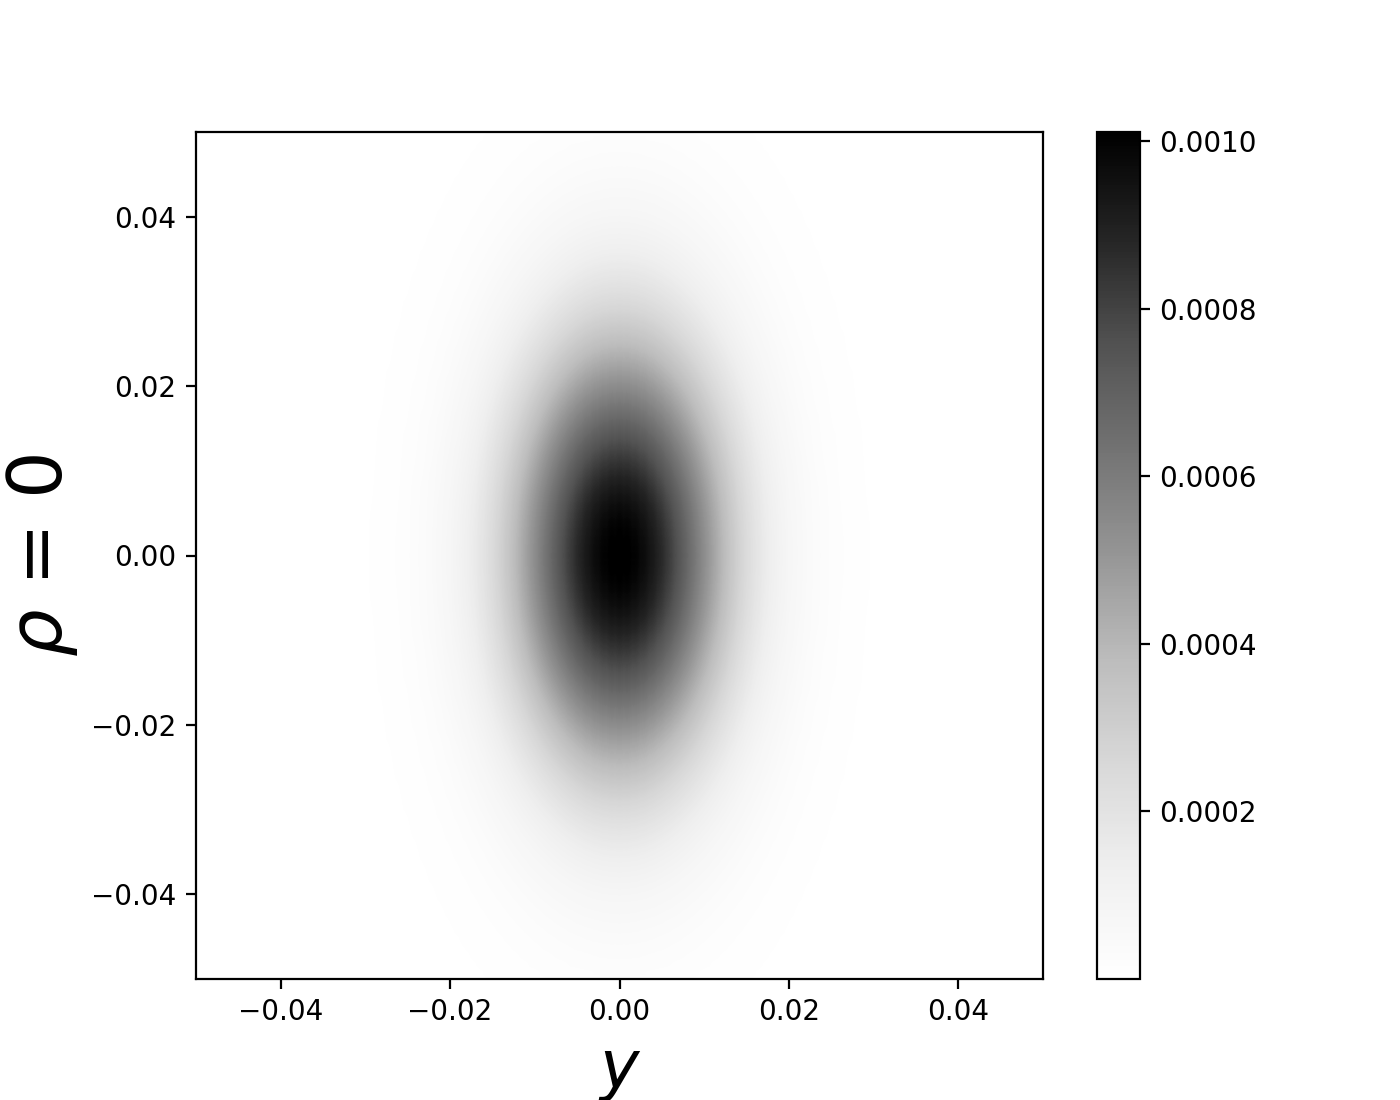
\includegraphics[width=\textwidth]{/home/hossein4527/MEGA/MEGAsync/Commit/University-Projects/MSc_Thesis/plots/Fig:(10a).png}
			\caption{$Joint PDF$}
			\label{fig:3.1.1}
		\end{subfigure}
		\hfill
		\begin{subfigure}[b]{0.24\textwidth}
			\renewcommand\thesubfigure{ii}
			\centering
			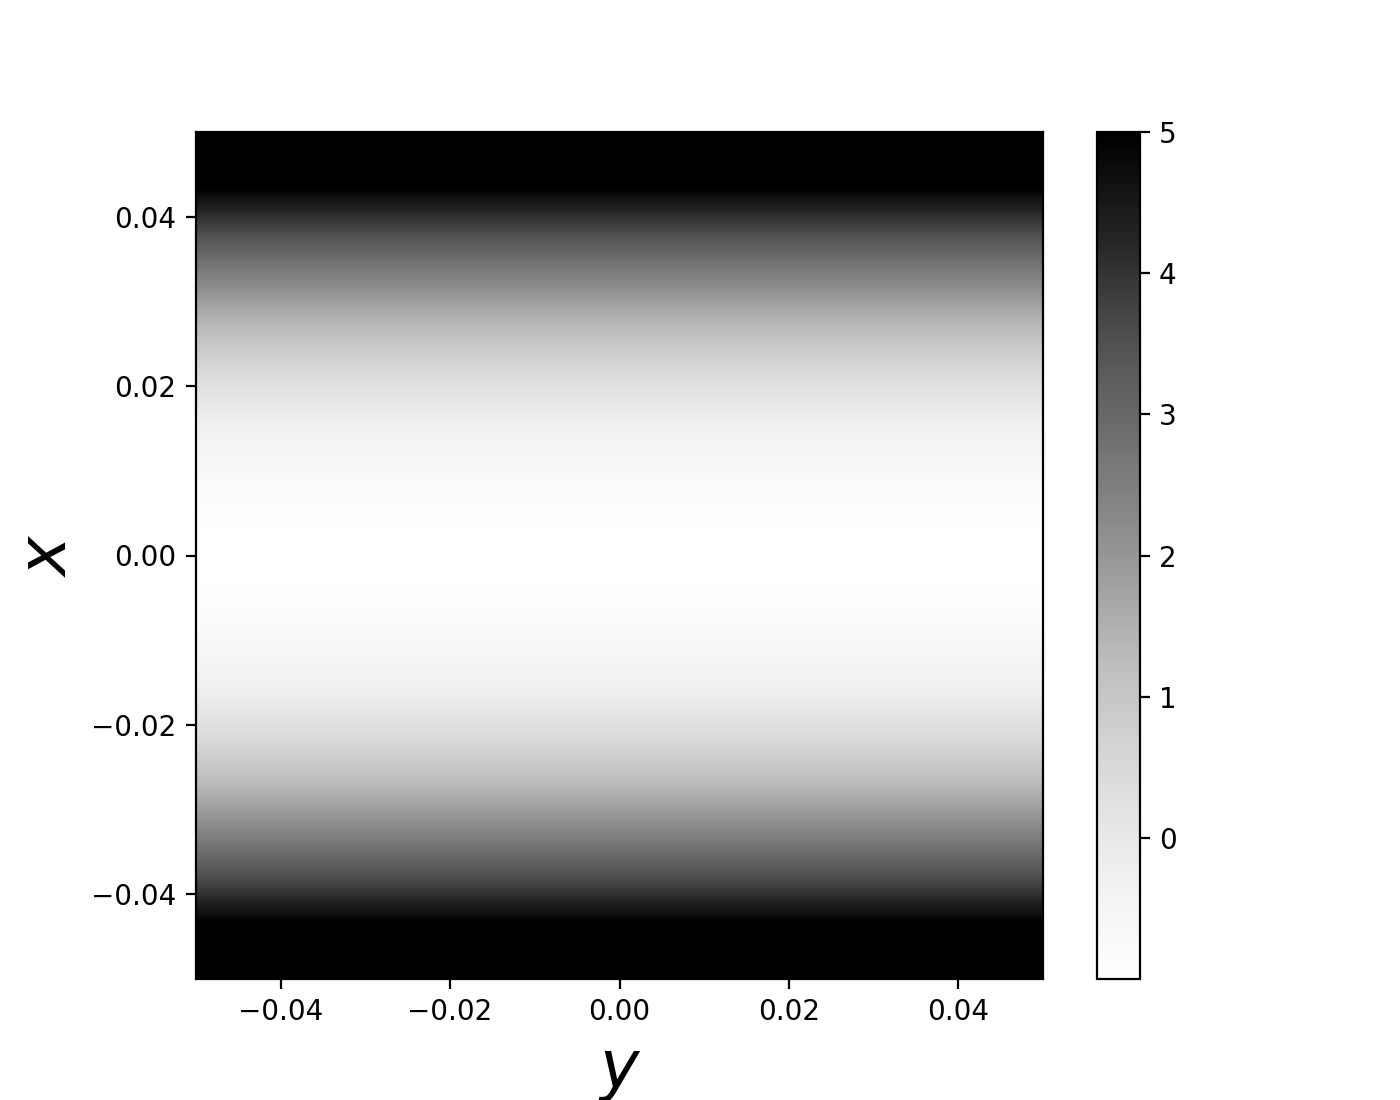
\includegraphics[width=\textwidth]{/home/hossein4527/MEGA/MEGAsync/Commit/University-Projects/MSc_Thesis/plots/Fig:(10b).png}
			\caption{$Q_{x:y}$}
			\label{fig:3.1.2}
		\end{subfigure}
		\hfill
		\begin{subfigure}[b]{0.24\textwidth}
			\renewcommand\thesubfigure{iii}
			\centering
			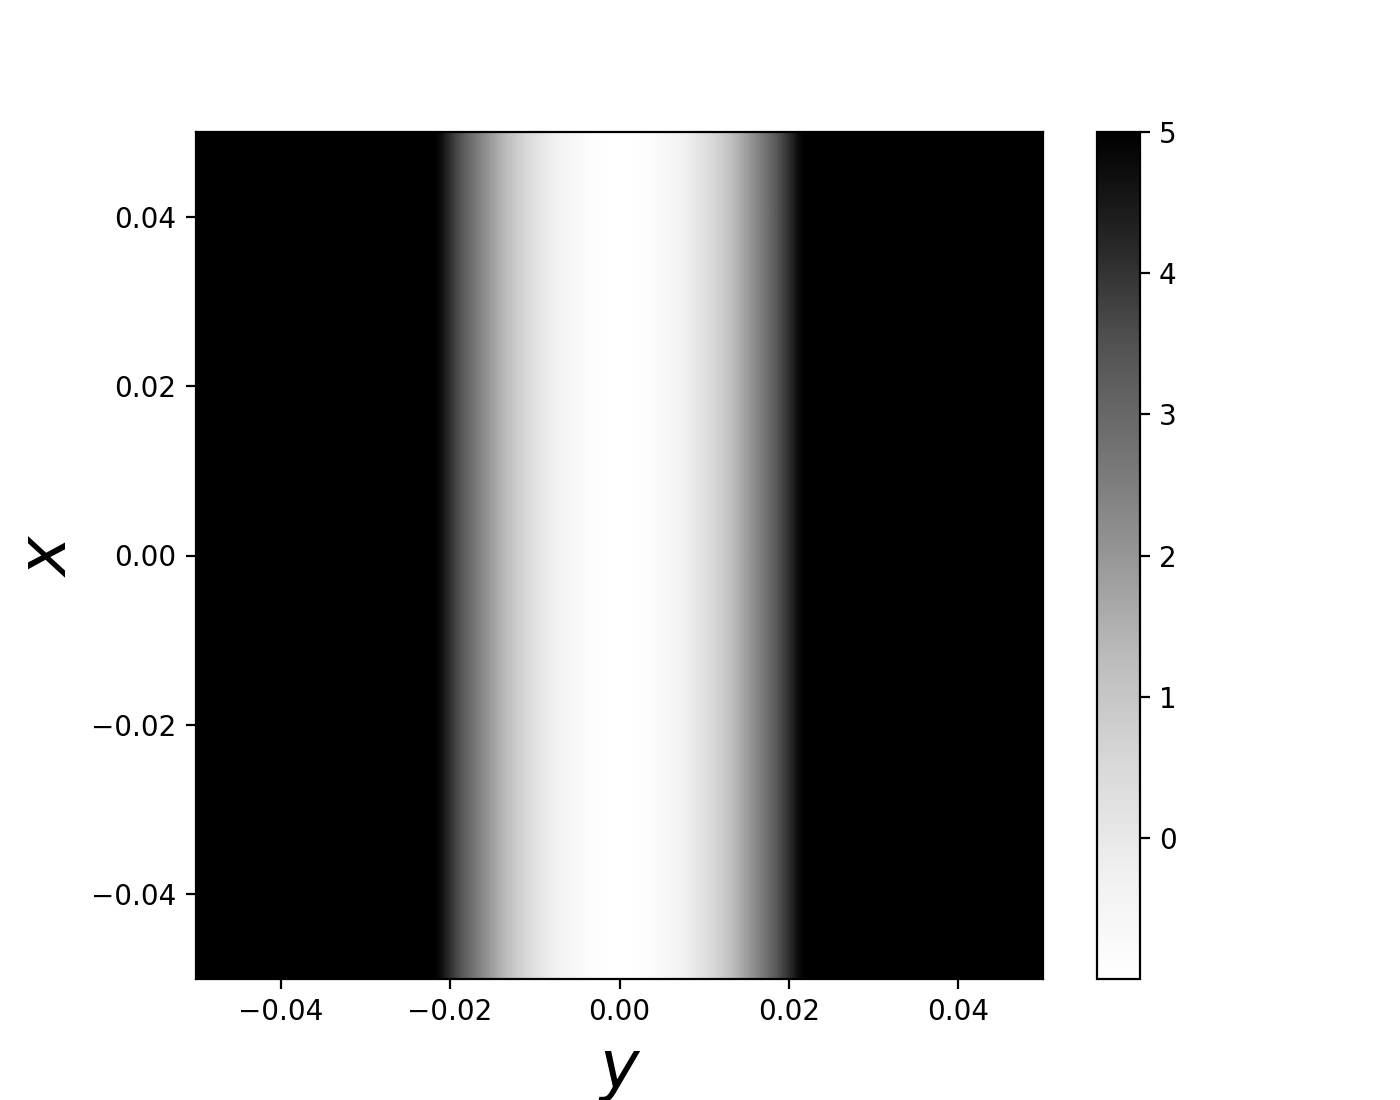
\includegraphics[width=\textwidth]{/home/hossein4527/MEGA/MEGAsync/Commit/University-Projects/MSc_Thesis/plots/Fig:(10c).png}
			\caption{$Q_{y:x}$}
			\label{fig:3.1.3}
		\end{subfigure}
		\hfill
		\begin{subfigure}[b]{0.24\textwidth}
			\renewcommand\thesubfigure{iv}
			\centering
			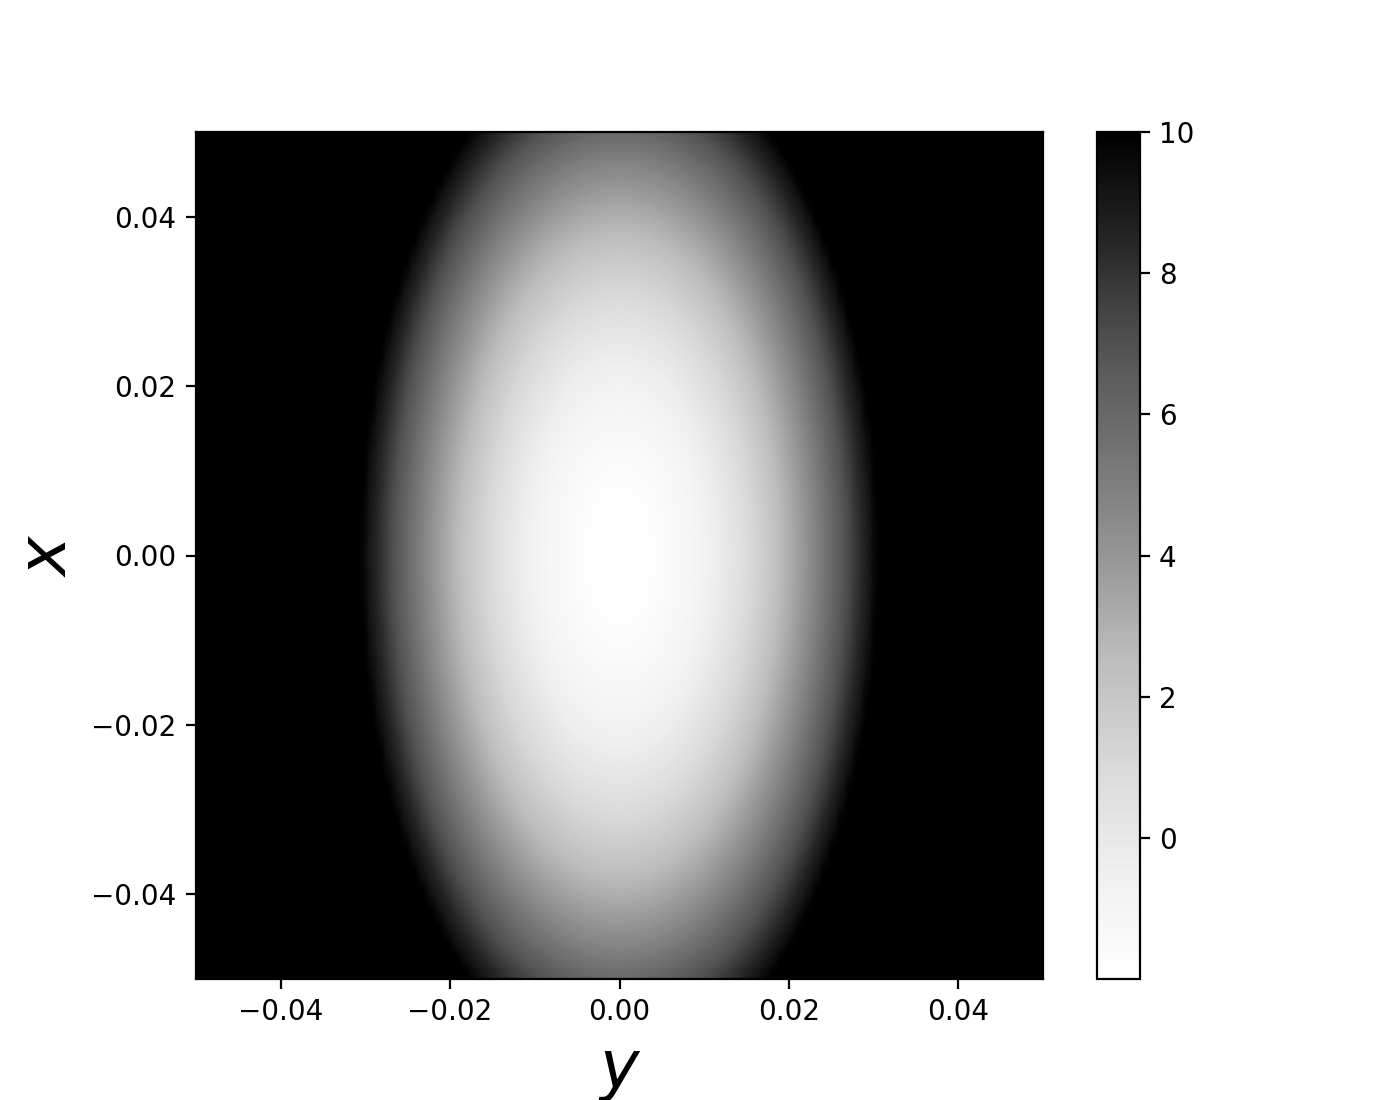
\includegraphics[width=\textwidth]{/home/hossein4527/MEGA/MEGAsync/Commit/University-Projects/MSc_Thesis/plots/Fig:(10d).png}
			\caption{$Q_{total}$}
			\label{fig:3.1.4}
		\end{subfigure}
		\caption{$\protect\rho =0$ و $\protect\sigma _{x}=2\protect\sigma _{y}$}
		\label{fig:3.1}
	\end{subfigure}
	\begin{subfigure}[b]{\textwidth}
		\renewcommand\thesubfigure{b}
		\begin{subfigure}[b]{0.24\textwidth}
			\renewcommand\thesubfigure{i}
			\centering
			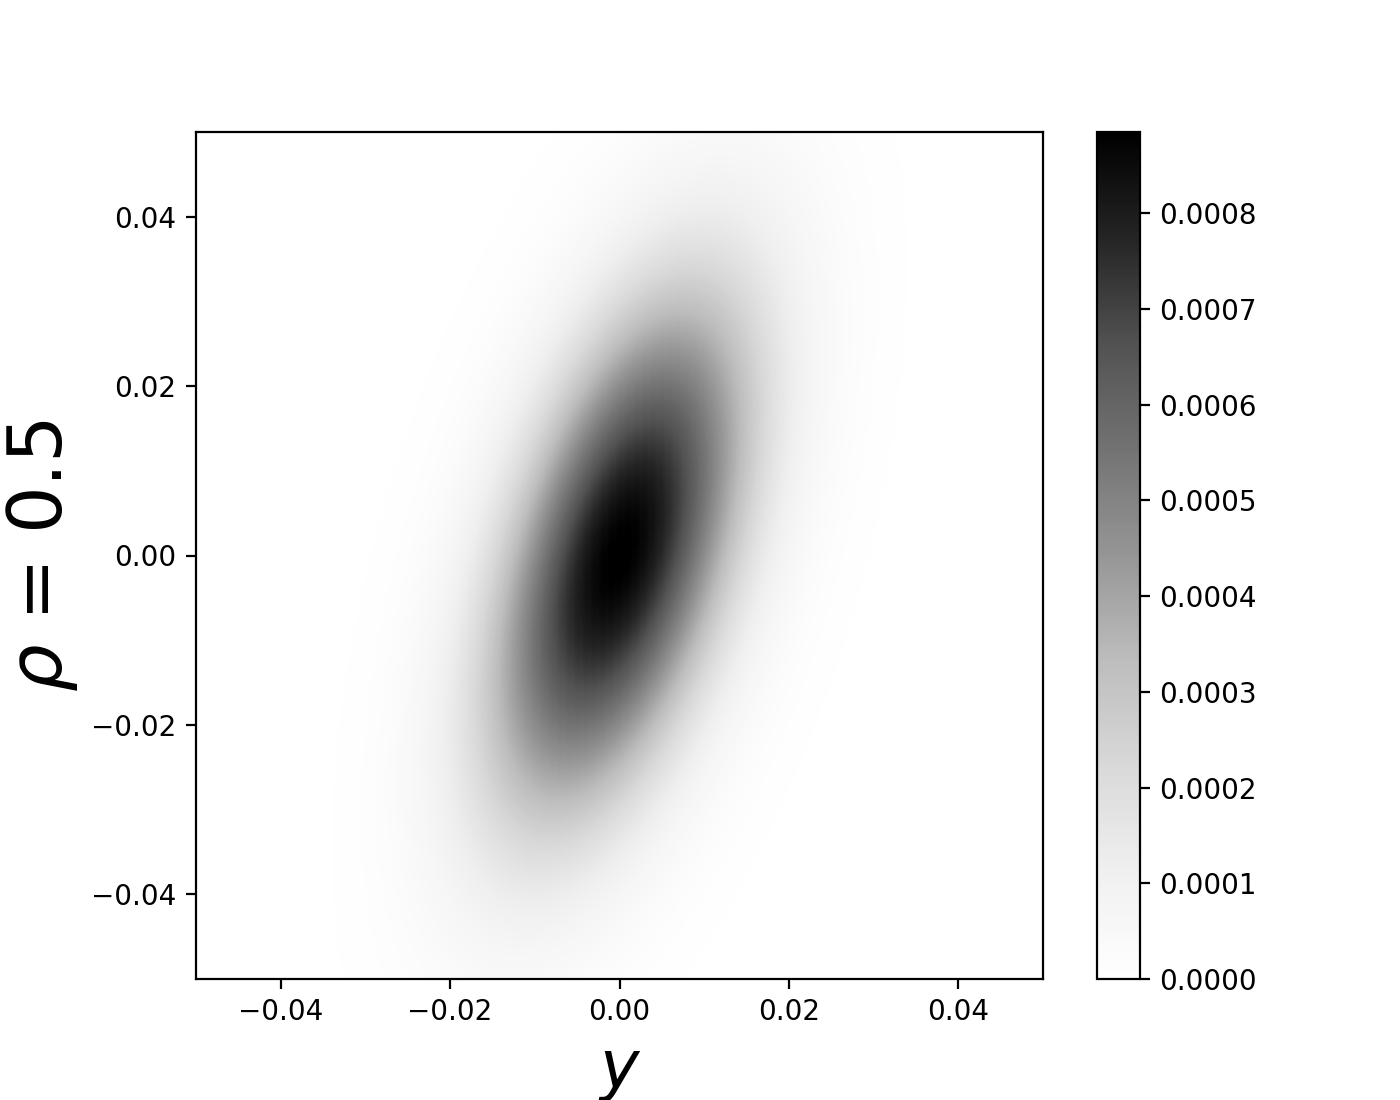
\includegraphics[width=\textwidth]{/home/hossein4527/MEGA/MEGAsync/Commit/University-Projects/MSc_Thesis/plots/Fig:(11a).png}
			\caption{$Joint PDF$}
			\label{fig:3.2.1}
		\end{subfigure}
		\hfill
		\begin{subfigure}[b]{0.24\textwidth}
			\renewcommand\thesubfigure{ii}
			\centering
			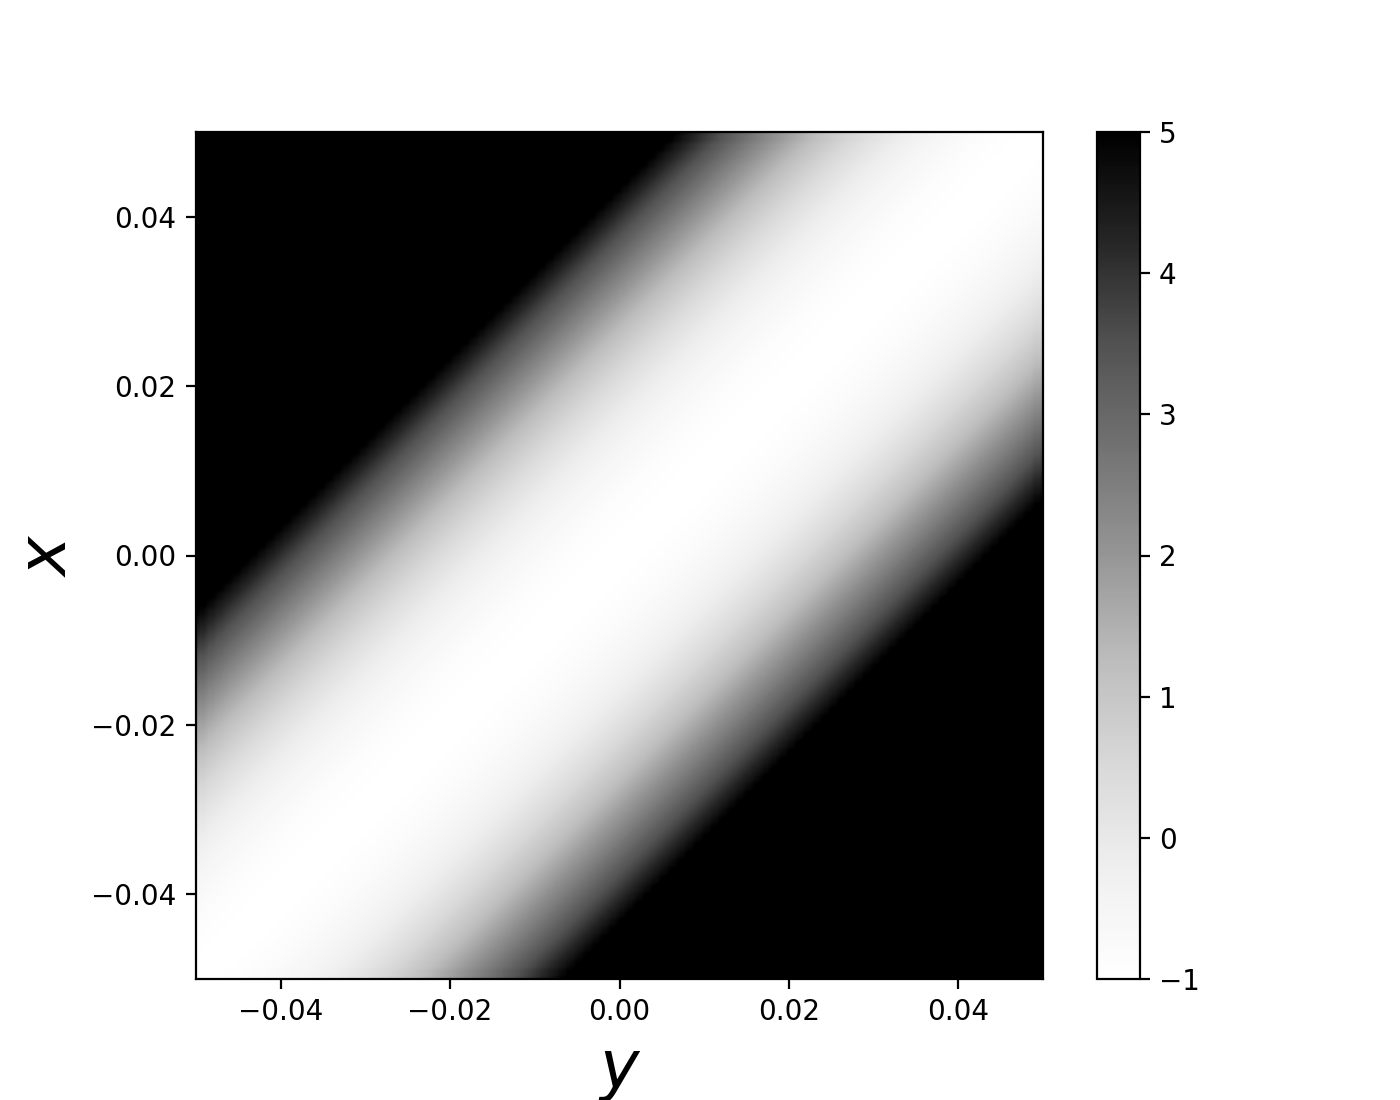
\includegraphics[width=\textwidth]{/home/hossein4527/MEGA/MEGAsync/Commit/University-Projects/MSc_Thesis/plots/Fig:(11b).png}
			\caption{$Q_{x:y}$}
			\label{fig:3.2.2}
		\end{subfigure}
		\hfill
		\begin{subfigure}[b]{0.24\textwidth}
			\renewcommand\thesubfigure{iii}
			\centering
			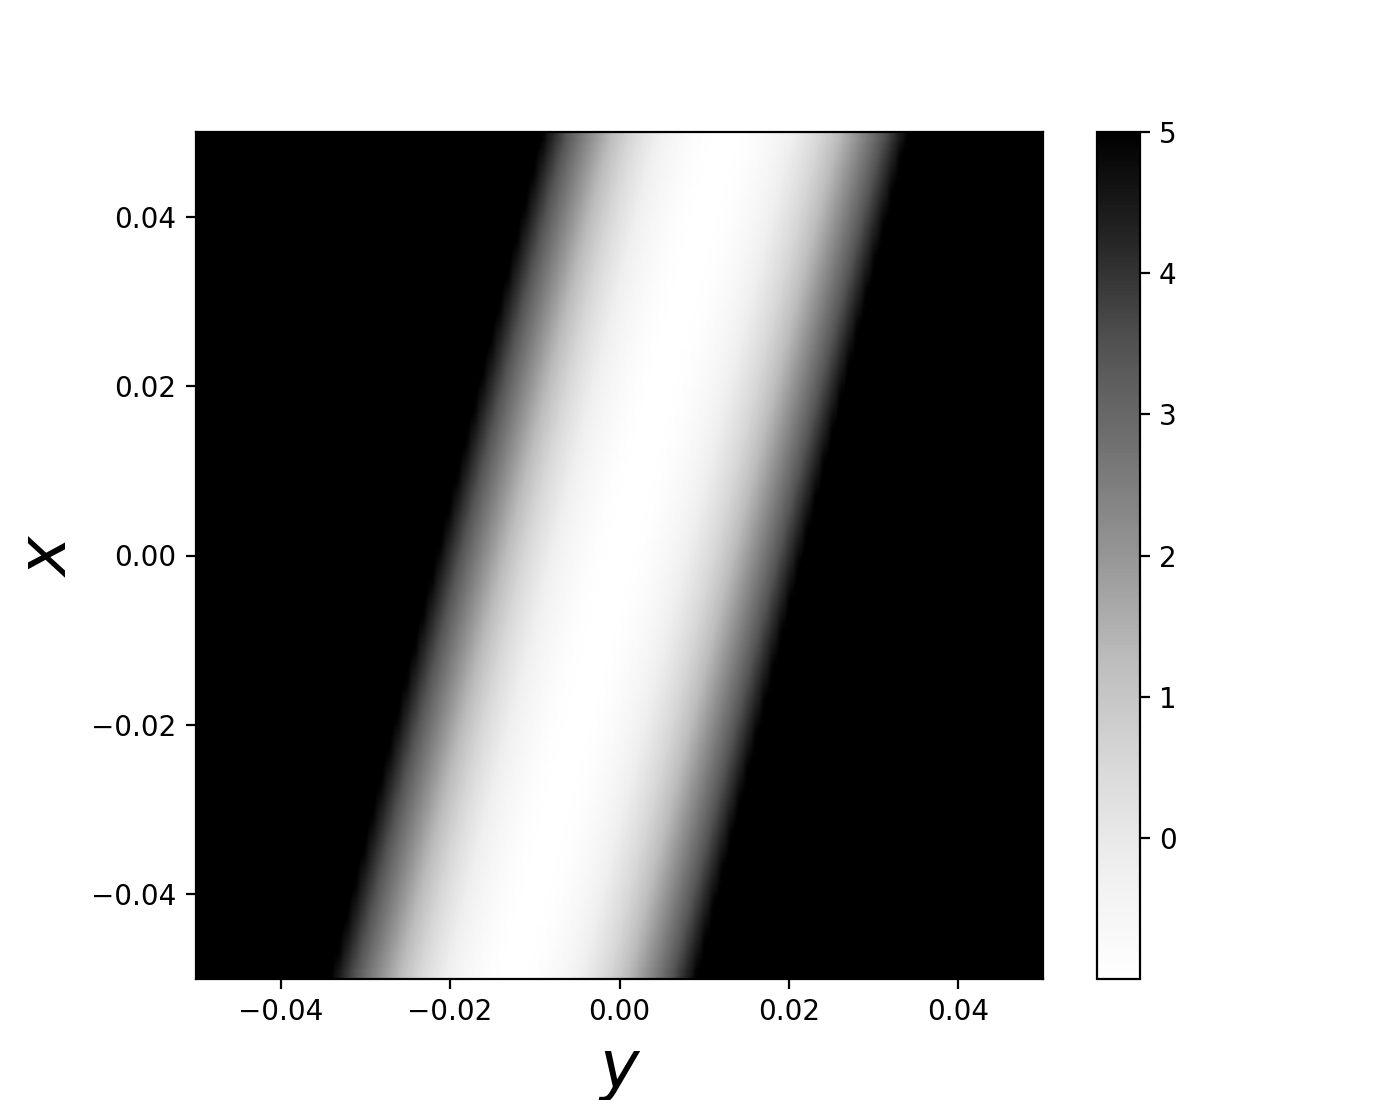
\includegraphics[width=\textwidth]{/home/hossein4527/MEGA/MEGAsync/Commit/University-Projects/MSc_Thesis/plots/Fig:(11c).png}
			\caption{$Q_{y:x}$}
			\label{fig:3.2.3}
		\end{subfigure}
		\hfill
		\begin{subfigure}[b]{0.24\textwidth}
			\renewcommand\thesubfigure{iv}
			\centering
			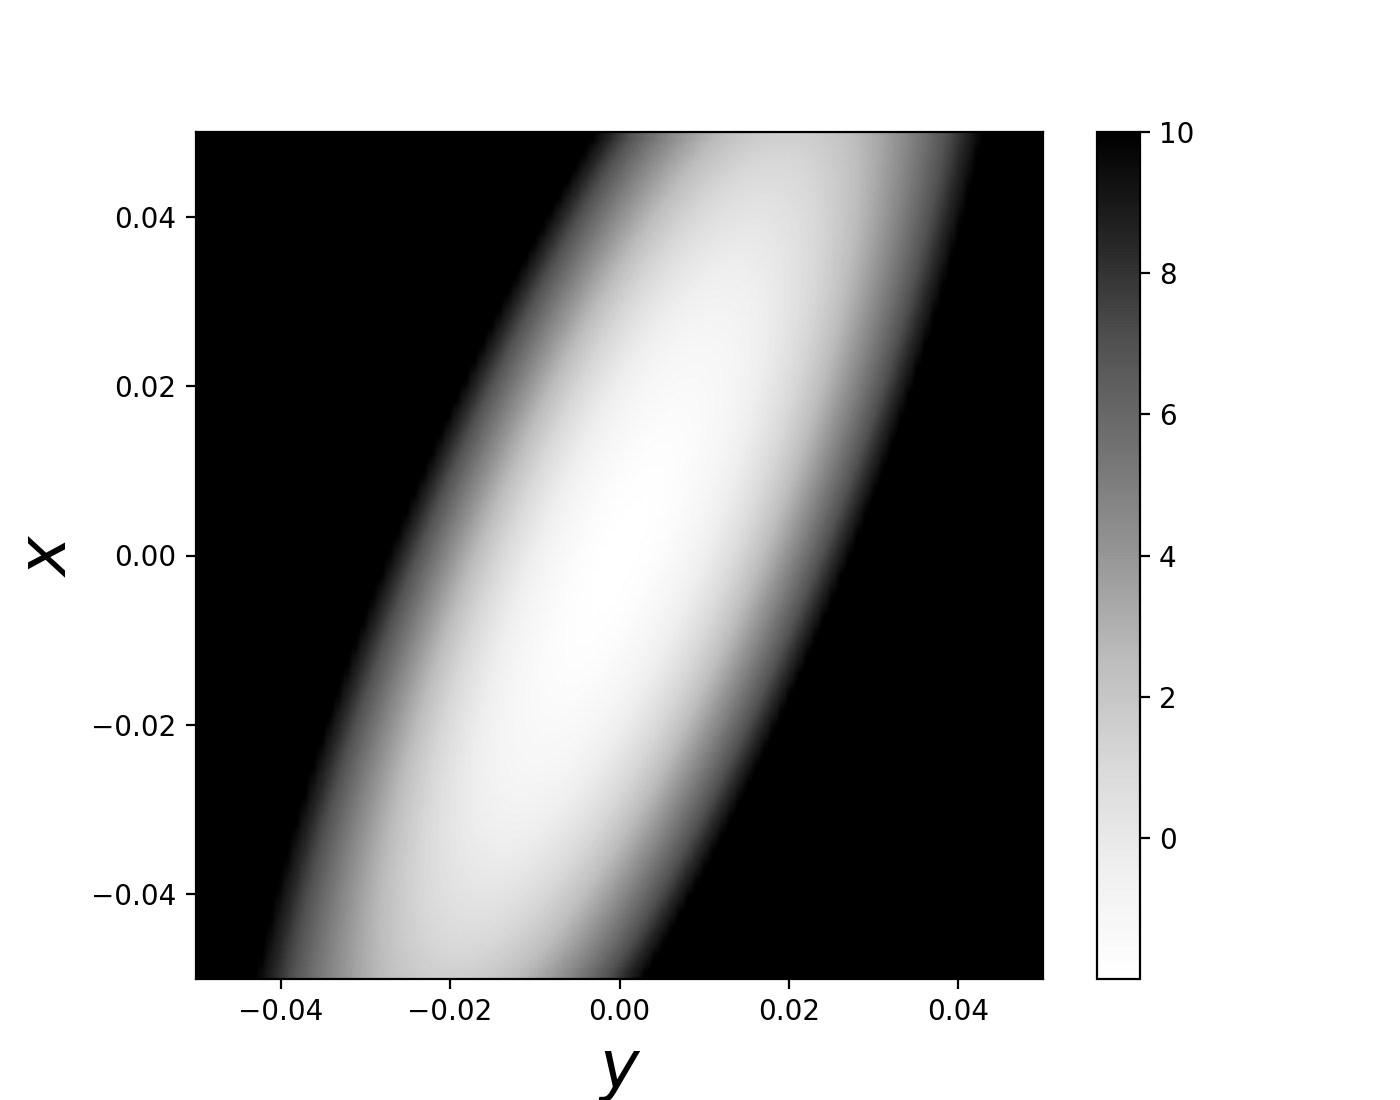
\includegraphics[width=\textwidth]{/home/hossein4527/MEGA/MEGAsync/Commit/University-Projects/MSc_Thesis/plots/Fig:(11d).png}
			\caption{$Q_{total}$}
			\label{fig:3.2.4}
		\end{subfigure}
		\caption{$\protect\rho =0.5$ و $\protect\sigma _{x}=2\protect\sigma _{y}$}
		\label{fig:3.2}
	\end{subfigure}
	\begin{subfigure}[b]{\textwidth}
		\renewcommand\thesubfigure{c}
		\begin{subfigure}[b]{0.24\textwidth}
			\renewcommand\thesubfigure{i}
			\centering
			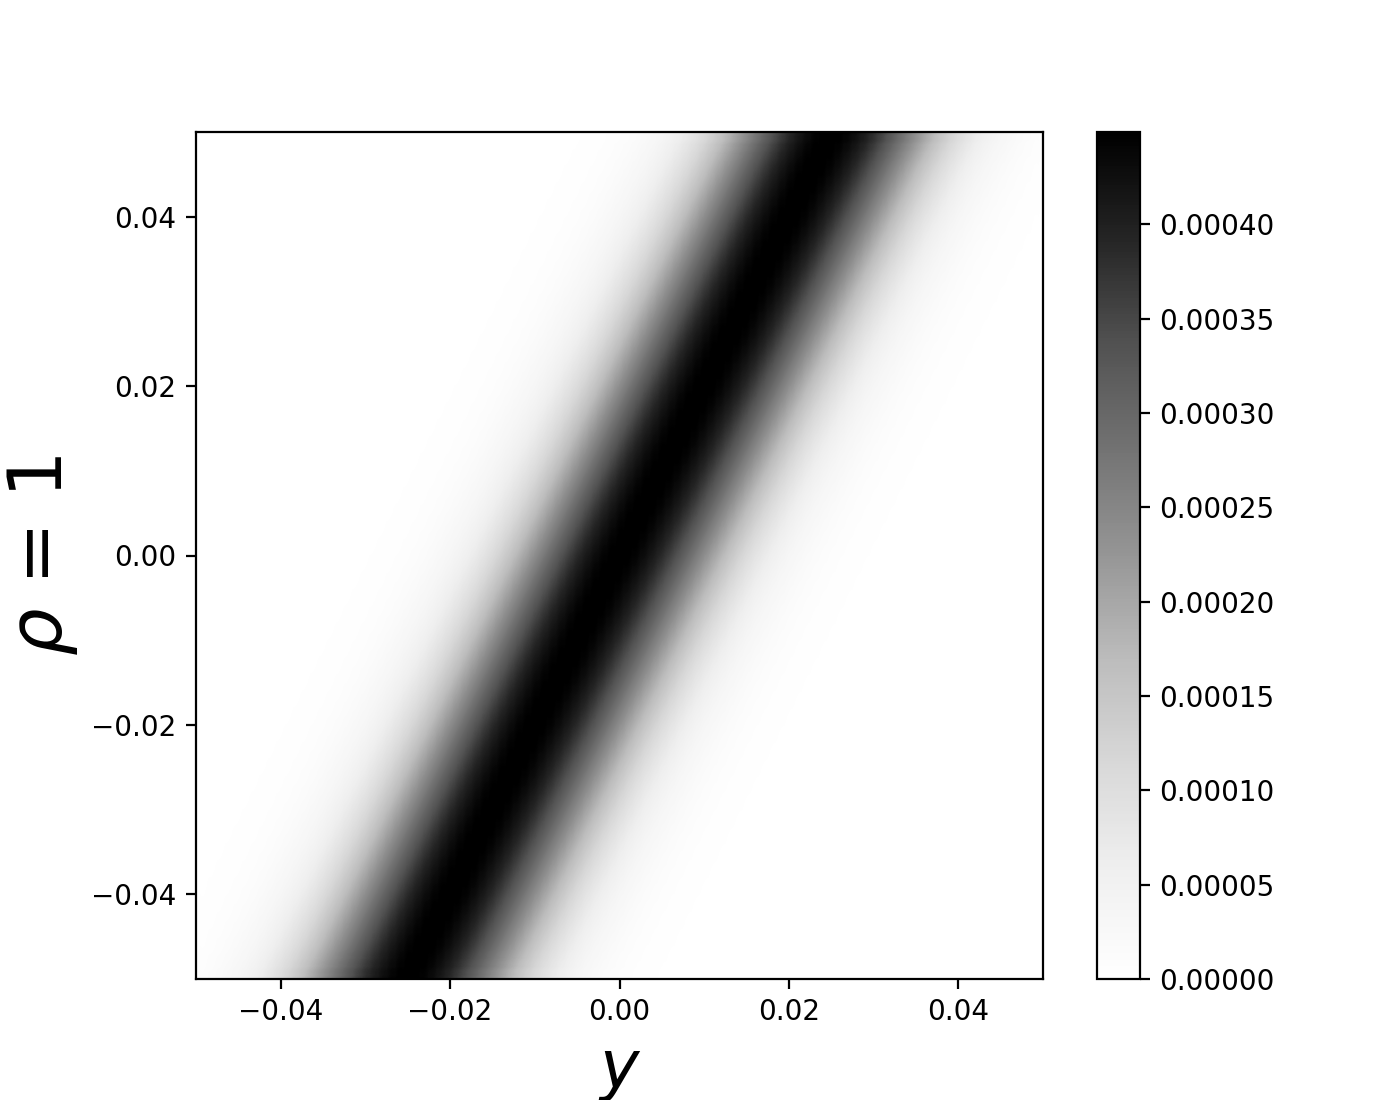
\includegraphics[width=\textwidth]{/home/hossein4527/MEGA/MEGAsync/Commit/University-Projects/MSc_Thesis/plots/Fig:(12a).png}
			\caption{$Joint PDF$}
			\label{fig:3.3.1}
		\end{subfigure}
		\hfill
		\begin{subfigure}[b]{0.24\textwidth}
			\renewcommand\thesubfigure{ii}
			\centering
			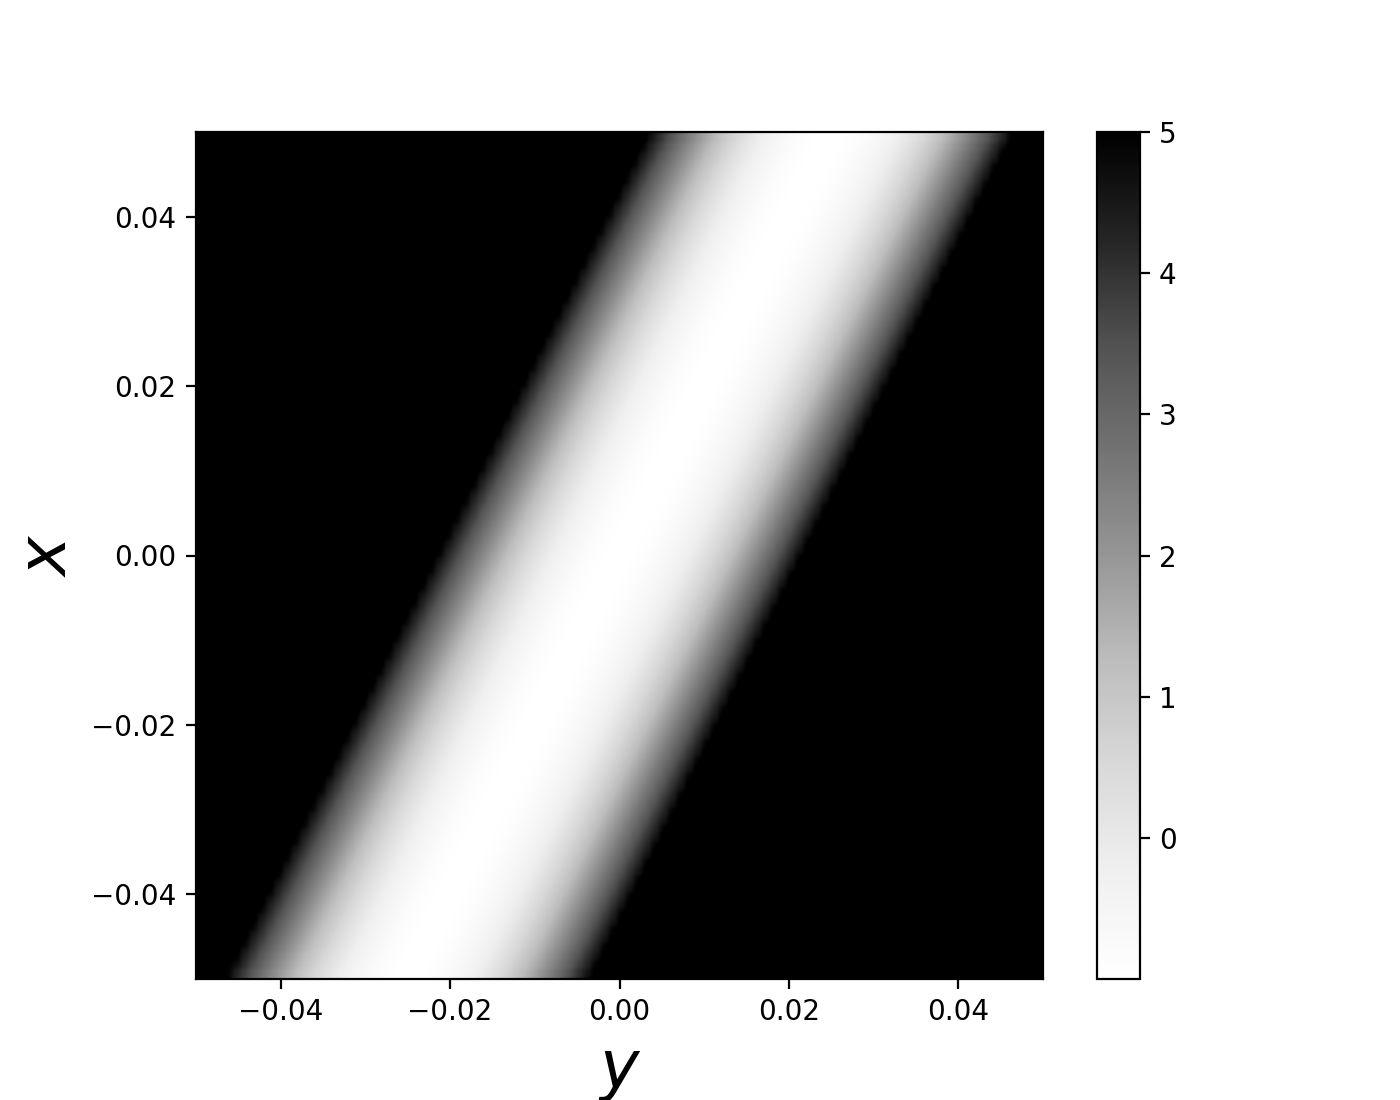
\includegraphics[width=\textwidth]{/home/hossein4527/MEGA/MEGAsync/Commit/University-Projects/MSc_Thesis/plots/Fig:(12b).png}
			\caption{$Q_{x:y}$}
			\label{fig:3.3.2}
		\end{subfigure}
		\hfill
		\begin{subfigure}[b]{0.24\textwidth}
			\renewcommand\thesubfigure{iii}
			\centering
			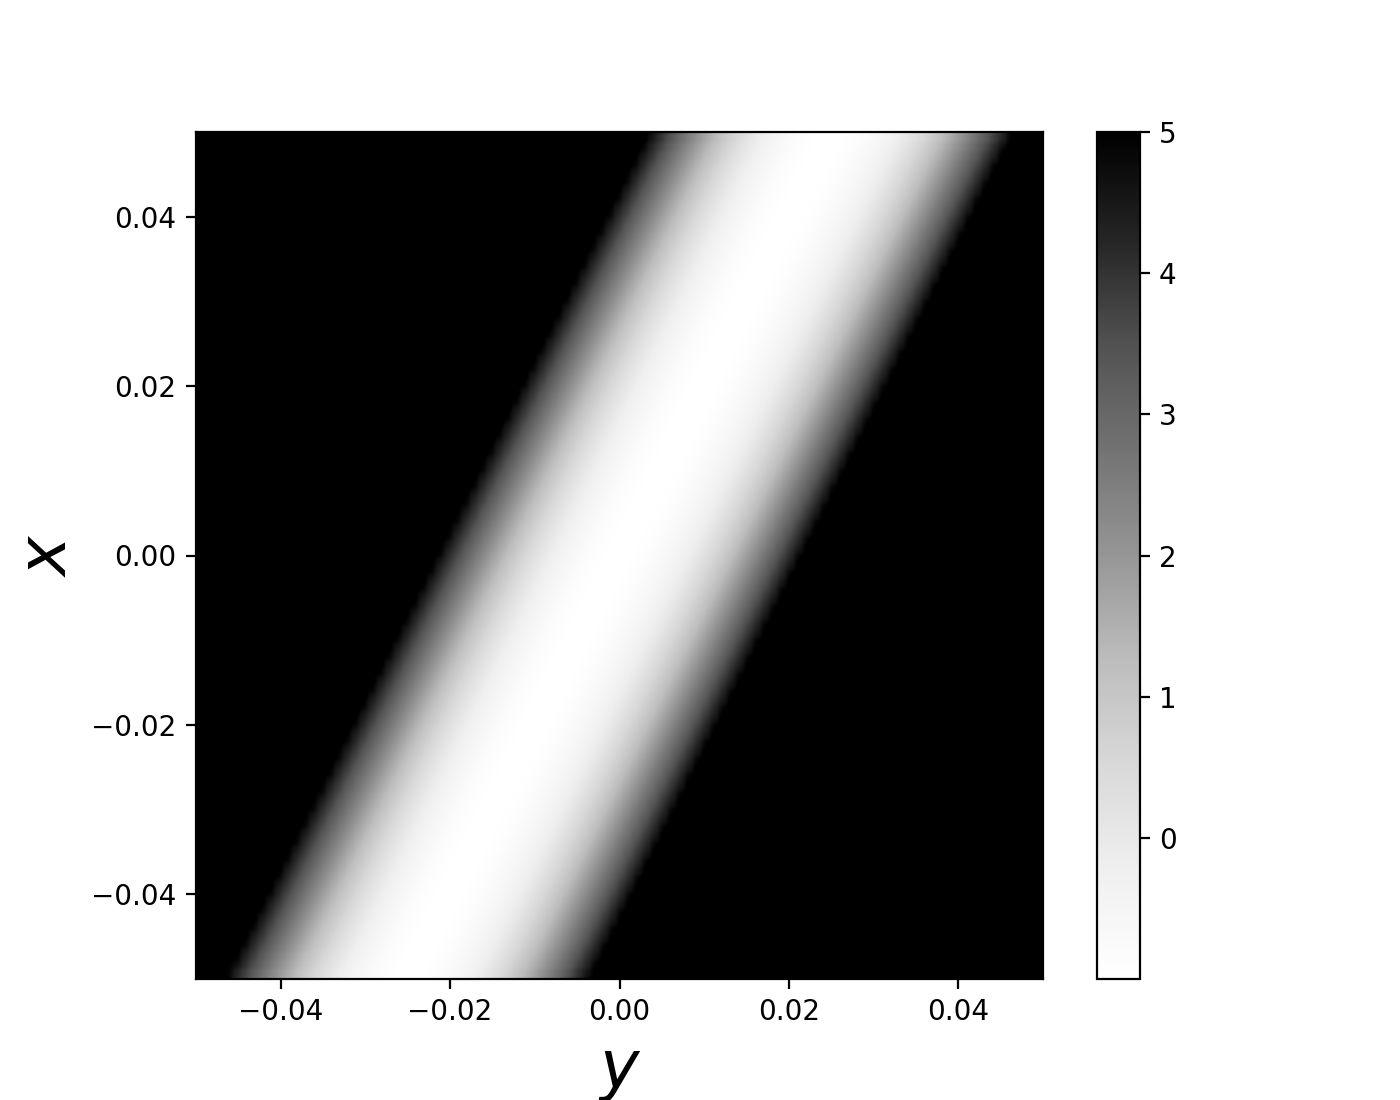
\includegraphics[width=\textwidth]{/home/hossein4527/MEGA/MEGAsync/Commit/University-Projects/MSc_Thesis/plots/Fig:(12c).png}
			\caption{$Q_{y:x}$}
			\label{fig:3.3.3}
		\end{subfigure}
		\hfill
		\begin{subfigure}[b]{0.24\textwidth}
			\renewcommand\thesubfigure{iv}
			\centering
			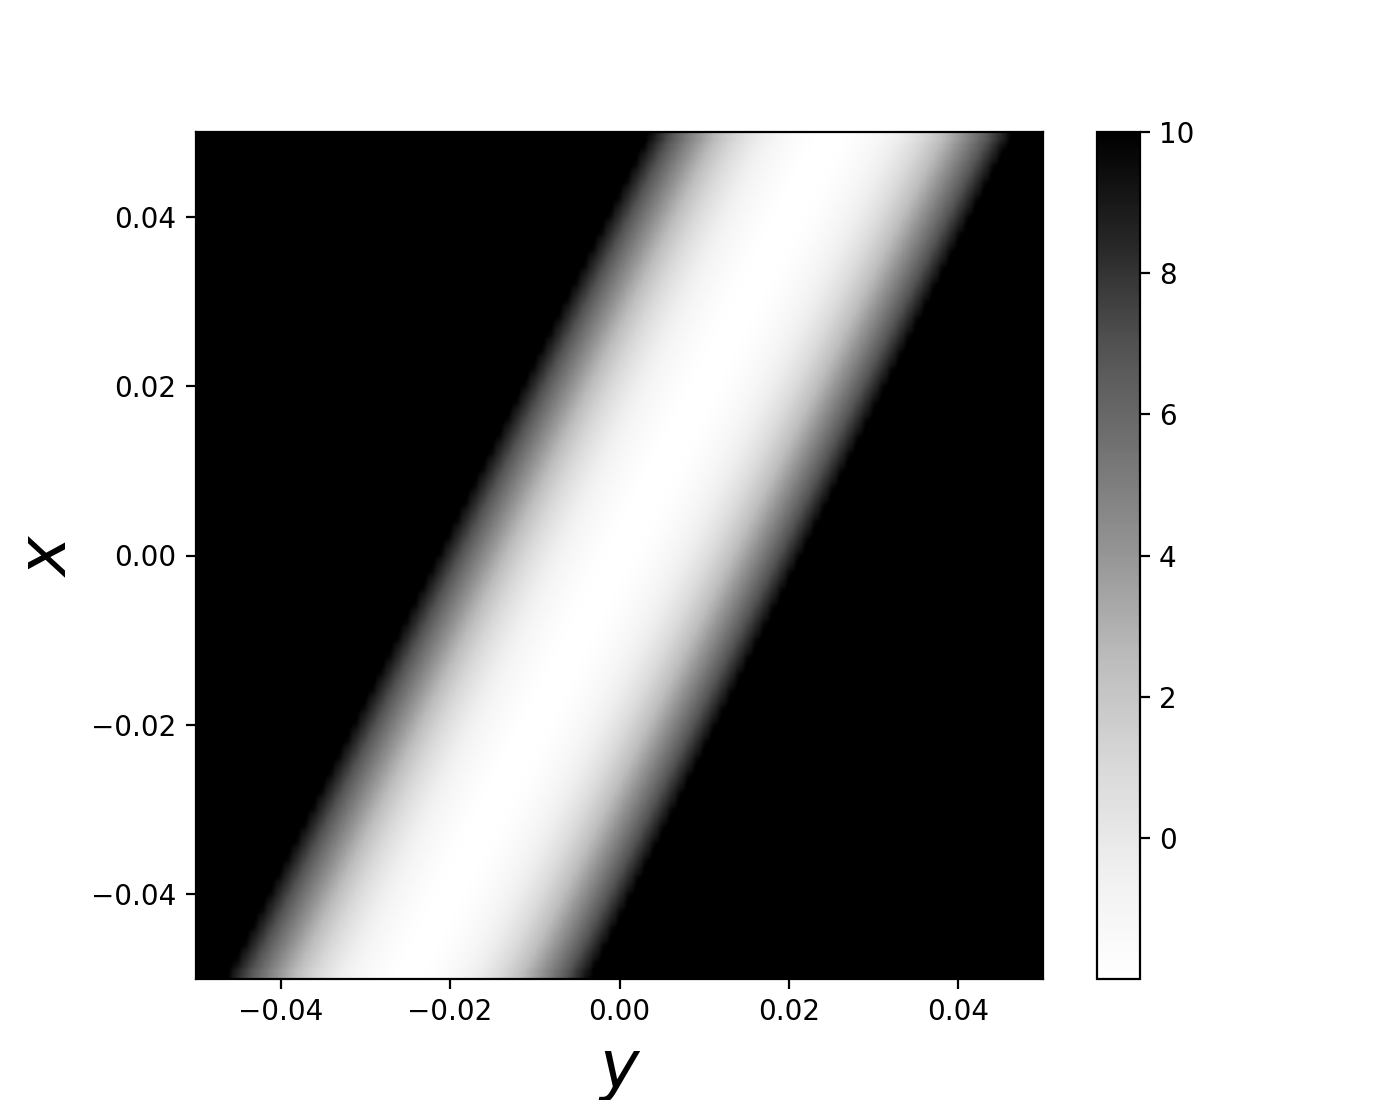
\includegraphics[width=\textwidth]{/home/hossein4527/MEGA/MEGAsync/Commit/University-Projects/MSc_Thesis/plots/Fig:(12d).png}
			\caption{$Q_{total}$}
			\label{fig:3.3.4}
		\end{subfigure}		
		\caption{$\protect\rho =1$ و $\protect\sigma _{x}=2\protect\sigma _{y}$}
		\label{fig:3.3}
	\end{subfigure}
	\caption{شکل سه بعدی گرمایی رسم شده برای تابع توزیع و پتانسیل های مربوطه برای
		$\protect\rho =0,0.5,1$ و $\protect\sigma _{x}=2\protect\sigma %
		_{y}$.}
	\label{fig:3t}
\end{figure}
اگر بخواهیم از دو ۳.۲.۲ و ۳.۲.۳ چکیده ای برای جمع بندی ارايه دهیم می توان به مطالب زیر اتکا کرد.
از شکل پتانسیل های کوانتومی، چه شرطی و چه کلی، می توان موضوعات جالبی را به دو بازار مورد نظر نسبت داد. 
الف) اگر پتانسیل کوانتومی کل دارای تقارنی نسبت به محور های مختصات بازار اول و دوم باشد، هر دو بازار دارای واریانسی برابر خواهند بود. اگر این تقارن دایروی باشد می توان نتیجه گرفت که دو بازار بدون همبستگی به کار خود ادامه  میدهند و زندگی هر کدام تاثیری بر دیگری ندارد. این عمل در واقعیت کمتر اتفاق می افتد ولی می توان بازار هایی را مثال زد که کمترین وابستگی ممکن را با یکدیگر در زمانی مشخص دارند. دقت کنیم که در مساله ما زمان و دینامیک جایگاهی ندارد و بررسی کردن دینامیک پتانسیل های مربوطه خارج از محدوده تحقیق و پژوهش این پایان نامه قرار دارد. پس برای ساده سازی اولیه، هر پتانسیلی که تقارن دایروی دارد یا به این تقارن نزدیک است را دو بازار کم وابسته می نامیم که جا برای تحقیق روی میزان این وابستگی باز باشد. 

ب) اگر پتانسیل کوانتومی کل تقارن دایروی خود را از دست بدهد، می توان نتیجه گرفت که میزان همبستگی دو بازار به یکدیگر بیشتر از صفر است. هر چه این پتانسیل از حالت دایروی بیشتر خارج شود و کشیدگی بیشتری پیدا کند دو ضریب همبستگی دو بازار بزرگتر خواهد بود. 

ج) از بین رفتن تقارن 
$r_1 \leftrightarrow r_2$
نتیجه می هد که با دو بازار با واریانس های متفاوت رو در رو هستیم. شکستگی این تقارن به سمت بازاری با واریانس بزرگ تر خواهد بود. 

برای استفاده از نتایج مطرح شده در مطالب فوق، باید این نتایج را در داده های واقعی مشاهده و مورد آزمایش قرار داد. به همین علت در بخش بعدی به بررسی نحوه محاسبه و تفسیر پتانسیل کوانتومی کل برای بازار های مختلف در کشورهای متفاوت می پردازیم. 
\newpage
\subsection{پتانسیل کوانتومی برای داده های واقعی}
در بخش قبلی به نحوه تفسیر اطلاعات از روی پتاننسیل کوانتومی کل محاسبه شده برای داده های ساختگی از روی یک مدل تابع توزیع مشترک گاوسی پرداختیم و نشان دادیم چگونه می توان اطلاعات آماری مورد نیاز را از روی پتانسیل های کوانتومی بدون کمک گرفتن از مکانیک آماری برداشت کرد. در این بخش می خواهیم به بررسی همین اطلاعات این بار برایی داده های واقعی بپردازیم. برای این کار ابتدا لام است بتوانیم بدون اشتباه و کمترین درصدی از خطا پتانسیل کوانتومی را برای داده های واقعی رسم کنیم. 

تنها داده مورد نیاز برای محاسبات ما داده های تاریخی قیمت بازار های دلخواه ما هستند. در این قسمت از داده های قیمتی روزانه استفاده شده است. بازارهای مورد بررسی در این پایان نامه شاخص های 
$S\&P500$، 
$Dow Jones$، 
$DAX$،
و 
$TOPIX$
 به ترتیب از کشور های آمریکا، آمریکا، آلمان و ژاپن انتخاب شده اند. برای هر چهار شاخص انتخاب شده داده ها از روزهایی برداشته شده است که همه آن ها همزمان داده ثبت کرده باشند. نمودار قیمت های این چهار شاخص در شکل زیر آورده شده است. حواسمان باشد که به دلیل ارز مبنای متفاوت در کشورهای متفاوت لازم بوده است که این داده ها را با مقیاس های متفاوت در یک شکل بیاوریم. پس در مرحله دیداری اولیه به سادگی قابل قیاس با یکدیگر نخواهند بود. 
 
 \begin{figure}[ptb]
 	\centering
 	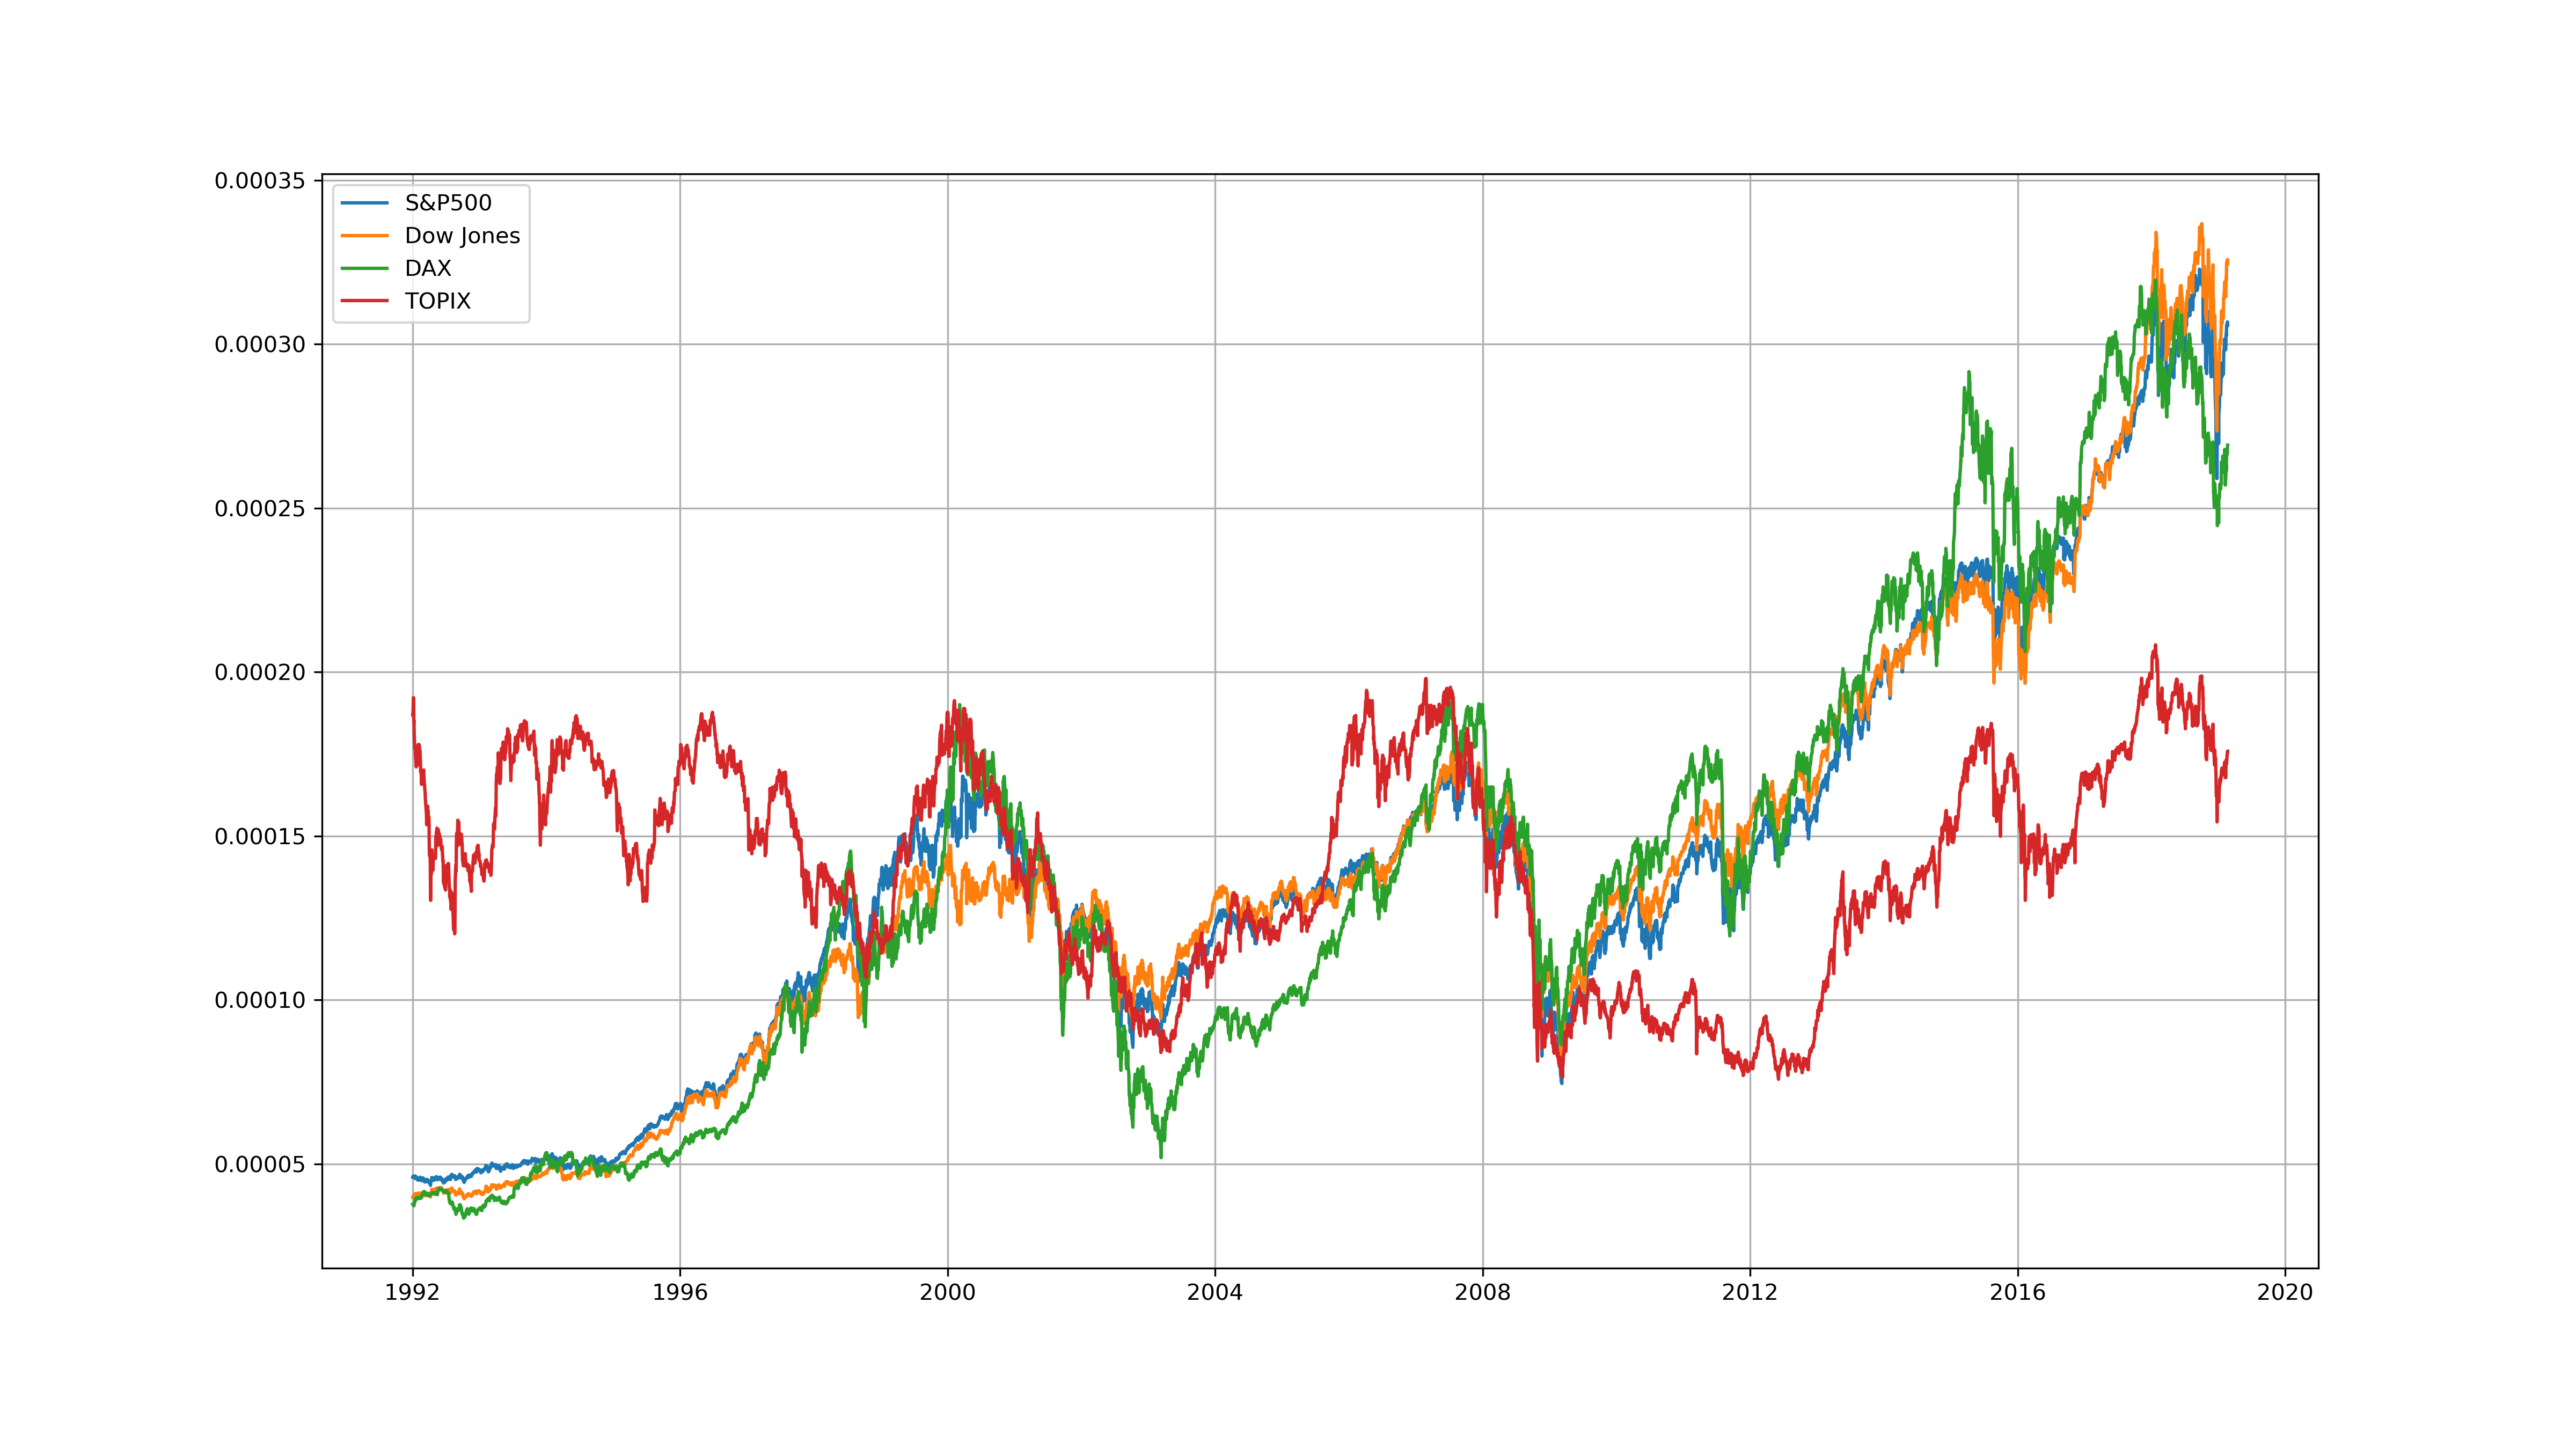
\includegraphics[width=\textwidth]{/home/hossein4527/MEGA/MEGAsync/Commit/University-Projects/MSc_Thesis/plots/fig3_11.png}
 	\caption{داده های قیمتی بازار های نشان داده شده در شکل برای بازه}
 	\label{fig:11}
 \end{figure}
برای محاسبه پتانسیل کوانتومی مشترک برای داده های نام برده به ترتیب هر یک از مراحل زیر انجام می شود. 
الف) از داده های قیمتی هر کدام از دو بازار مورد نظر برای محاسبه پتانسیل مشترک آن ها، سود لگاریتمی محاسبه می شود.

ب) از داده های سود لگاریتمی هر دو بازار تابع توزیع مشترک بین آن دو محاسبه می شود. 

ج) تابع توزیع محاسبه شده توسط یک کرنل گاوسی صاف و هموار می شود.

د) از تابع توزیع مشترک محاسبه شده توسط معادله ی 
\ref{eq:3.5}
پتانسیل کوانتومی مشترک محاسبه می شود. 

برای یافتن درک بهتر از شکل های داده واقعی نسبت به شکل های مدل ساختگی از بخش قبلی، بهتر است ابتدا پتانسیل کوانتومی مشترکی محاسبه شود که هر دو مختصات بازار آن را یک داده تشکیل دهد. برای مثال پتانسیل کوانتومی محاسبه شده توسط کد های برنامه نویسی ما برای بازار اول
$S\&P500$
و بازار دوم هم
$S\&P500$
همانند شکل 
\ref{fig:12}
خواهد شد.
 \begin{figure}[ptb]
	\centering
	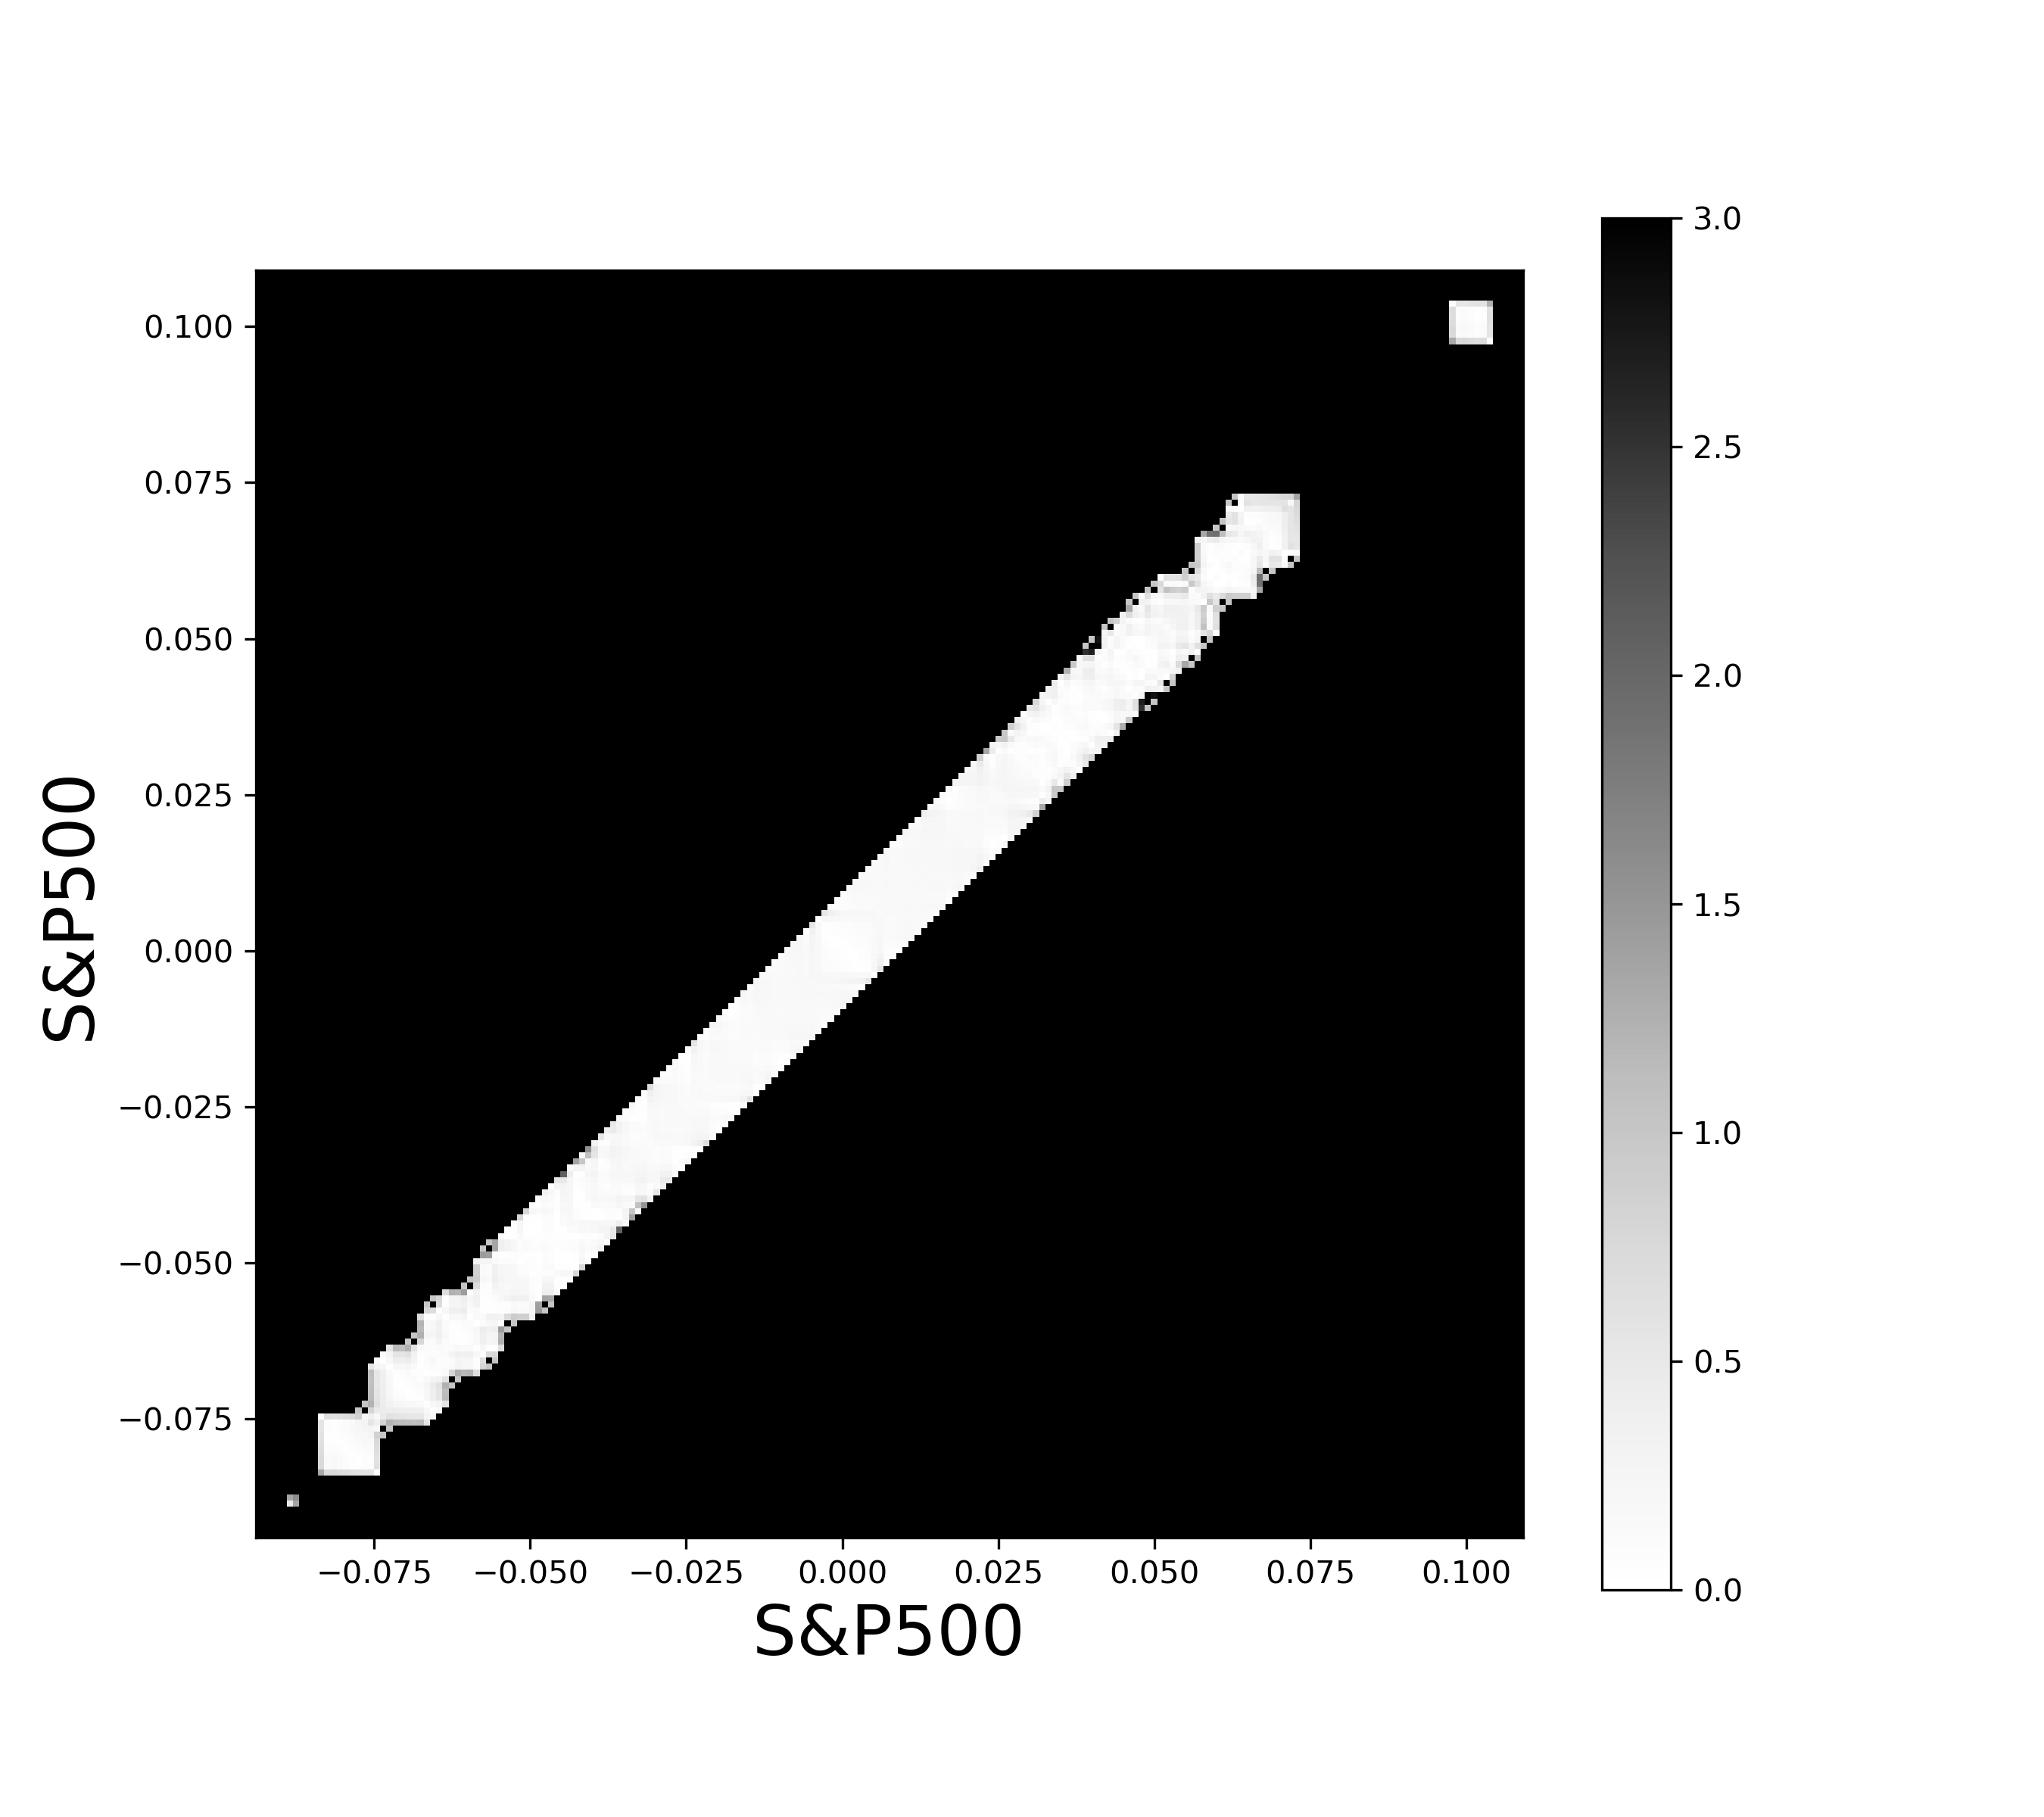
\includegraphics[width=\textwidth]{/home/hossein4527/MEGA/MEGAsync/Commit/University-Projects/MSc_Thesis/plots/snp_snp.png}
	\caption{پتانسیل کوانتومی مشترک محاسبه شده برای بازار های نشان داده شده در مختصات.}
	\label{fig:12}
\end{figure}
نکاتی که باید در مورد شکل 
\ref{fig:12}
متذکر شویم این است که اعداد نمایش داده شده در هر یک از مختصات نمایان گر سود و زیان مربوط به بازار مختصات مربوطه است. قسمت های سفید رنگ چاه پتانسیل سه بعدی هستند که هرچه به سمت قسمت های خاکستری و سپس مشکی تر نزدیک می شویم، مقدار پتانسیل زیاد تر شده تا جاییکه به دبواره های پتانسیل که رنگی سیاه دارند میرسیم. اعداد نمایش داده شده در کنار شکل به صورت مقیاسی بوده و حاکی از کم و زیاد بودن پتانسیل در خانه های رنگی مربوطه هستند به طوریکه سفید به منظور عدم وجود پتانسیل و سیاه به منظور وجود سد عظیمی از پتانسیل است. 
با مقایسه شکل 
\ref*{fig:12}
با شکل
\ref{fig:2.3.4} 
و 
\ref{fig:3.3.4}
می توان به سادگی تفاوت بین نمودار های توابع تحلیلی و داده های واقعی را دریافت.
پس حالا که فهمیدیم پتانسیل کوانتومی مشترک برای دو بازار به شدت وابسته و دارای واریانس یکسان برای داده های واقعی چگونه است و به همراه داشتن نمونه شکل های مطرح شده در مدل گاوسی، می توان به تحلیل و بررسی هر یک از پتانسیل های کوانتومی مشترک محاسبه شده برای هر دو بازار دلخواه مطرح شده پرداخت.
با توجه به شکل های بدست آمده از داده های موجود، می توان هر دو تایی از این بازار ها را تحت زیرمجموعه ای از سه گروه کم وابسته، وابسته و به شدت وابسته تقسیم بندی کرد. 
هر کدام از این شکل ها در یک بخش تفسیر شده اند.

\textbf{
الف) پتانسیل کوانتومی مشترک محاسبه شده برای بازار های 
$TOPIX$
و 
$DAX$
به عنوان دو بازار کم وابسته:
}


 \begin{figure}[ptb]
	\centering
	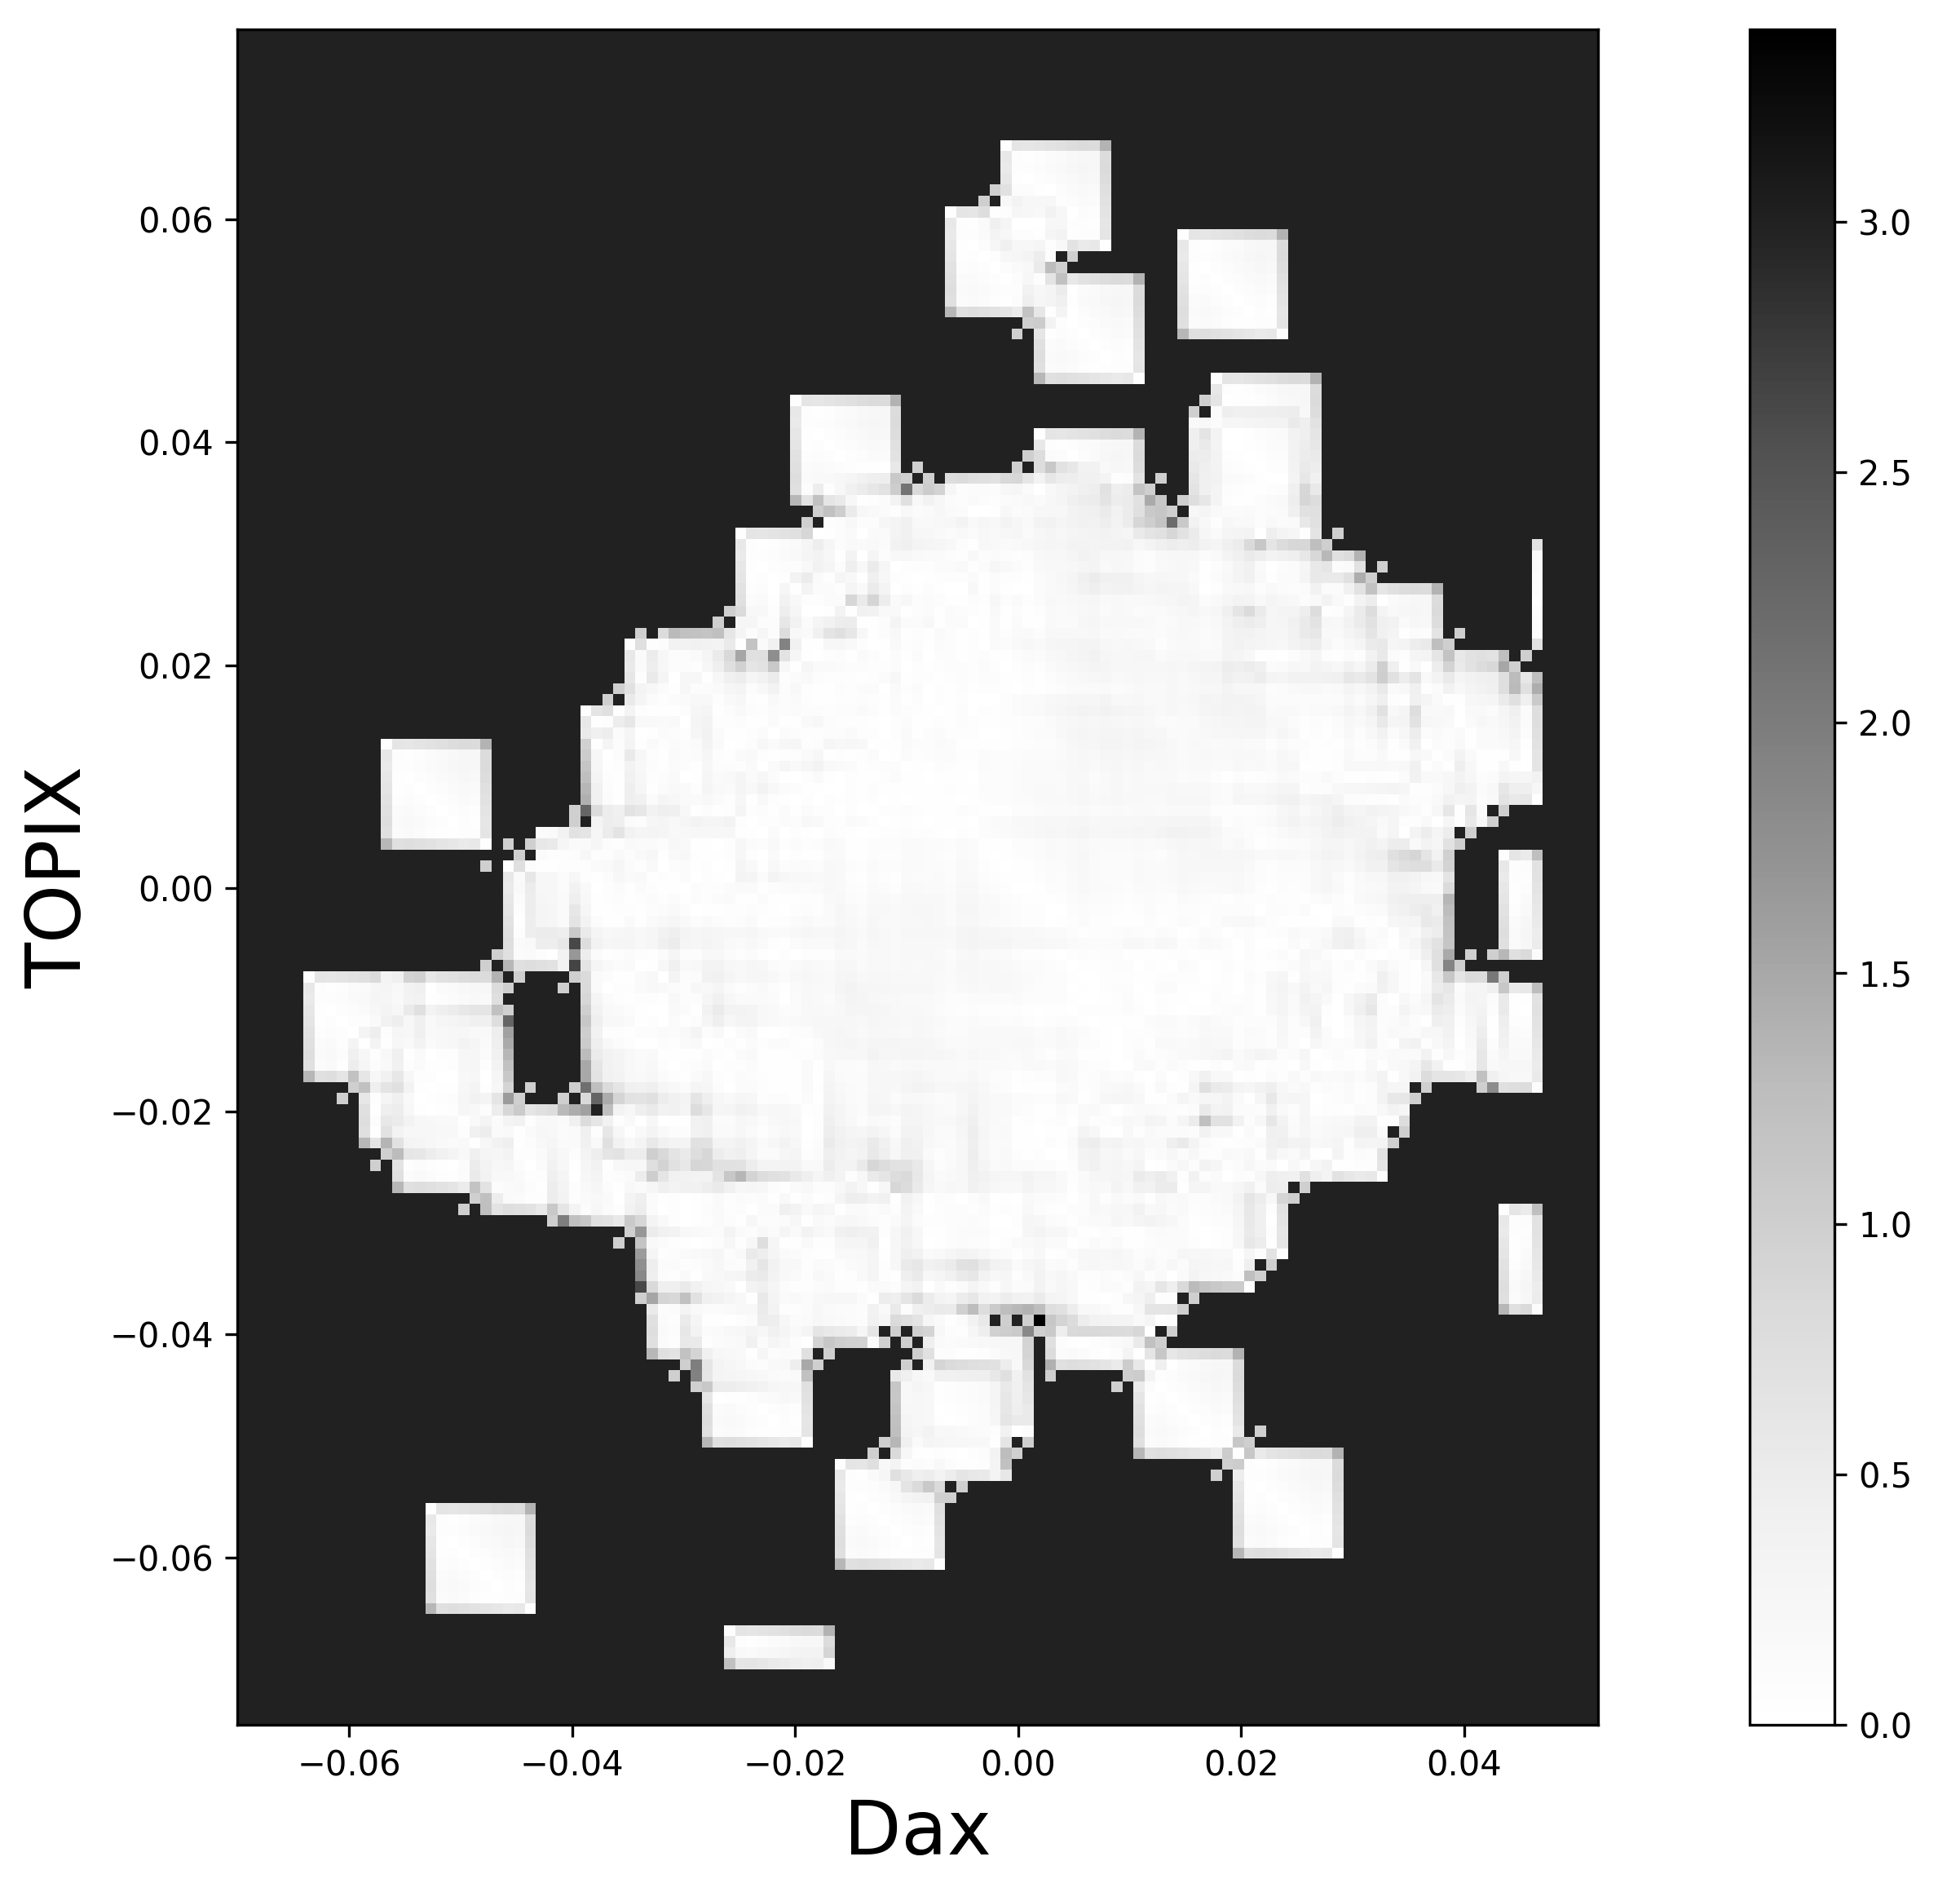
\includegraphics[width=\textwidth]{/home/hossein4527/MEGA/MEGAsync/Commit/University-Projects/MSc_Thesis/plots/Dax_Topix.png}
	\caption{پتانسیل کوانتومی مشترک محاسبه شده برای بازار های نشان داده شده در مختصات.}
	\label{fig:13}
\end{figure}
همانطور که در شکل
\ref{fig:13}
به وضوح پیداست، هر کسی با مقایسه این شکل و شکل 
\ref{fig:2t}
در می یابد که پتانسیل کوانتومی محاسبه شده برای 
$DAX$
و
$TOPIX$
همانند پتانسیل کوانتومی برای ضریب همبستگی 
$\rho=0$
در مدل گاوسی مطرح شده است. پتانسیل کوانتومی برای این دو بازار تمایل به یک تقارن دایروی دارد و به سمت هیچ یک از مختصات به صورت خاص کشیدگی ندارد. از این شکل می توان در یافت که تغییر در مقدار سود و زیان هر یک از این بازار ها، تاثیری بر بازار دیگر ندارد و دو بازار به صورت مستقل از یکدیگر زندگی میکنند.
\newline
\newline
ب) پتانسیل کوانتومی مشترک محاسبه شده برای بازارهای 
$S\&P500$
و
$DAX$
به عنوان دو بازار وابسته:
 \begin{figure}[ptb]
	\centering
	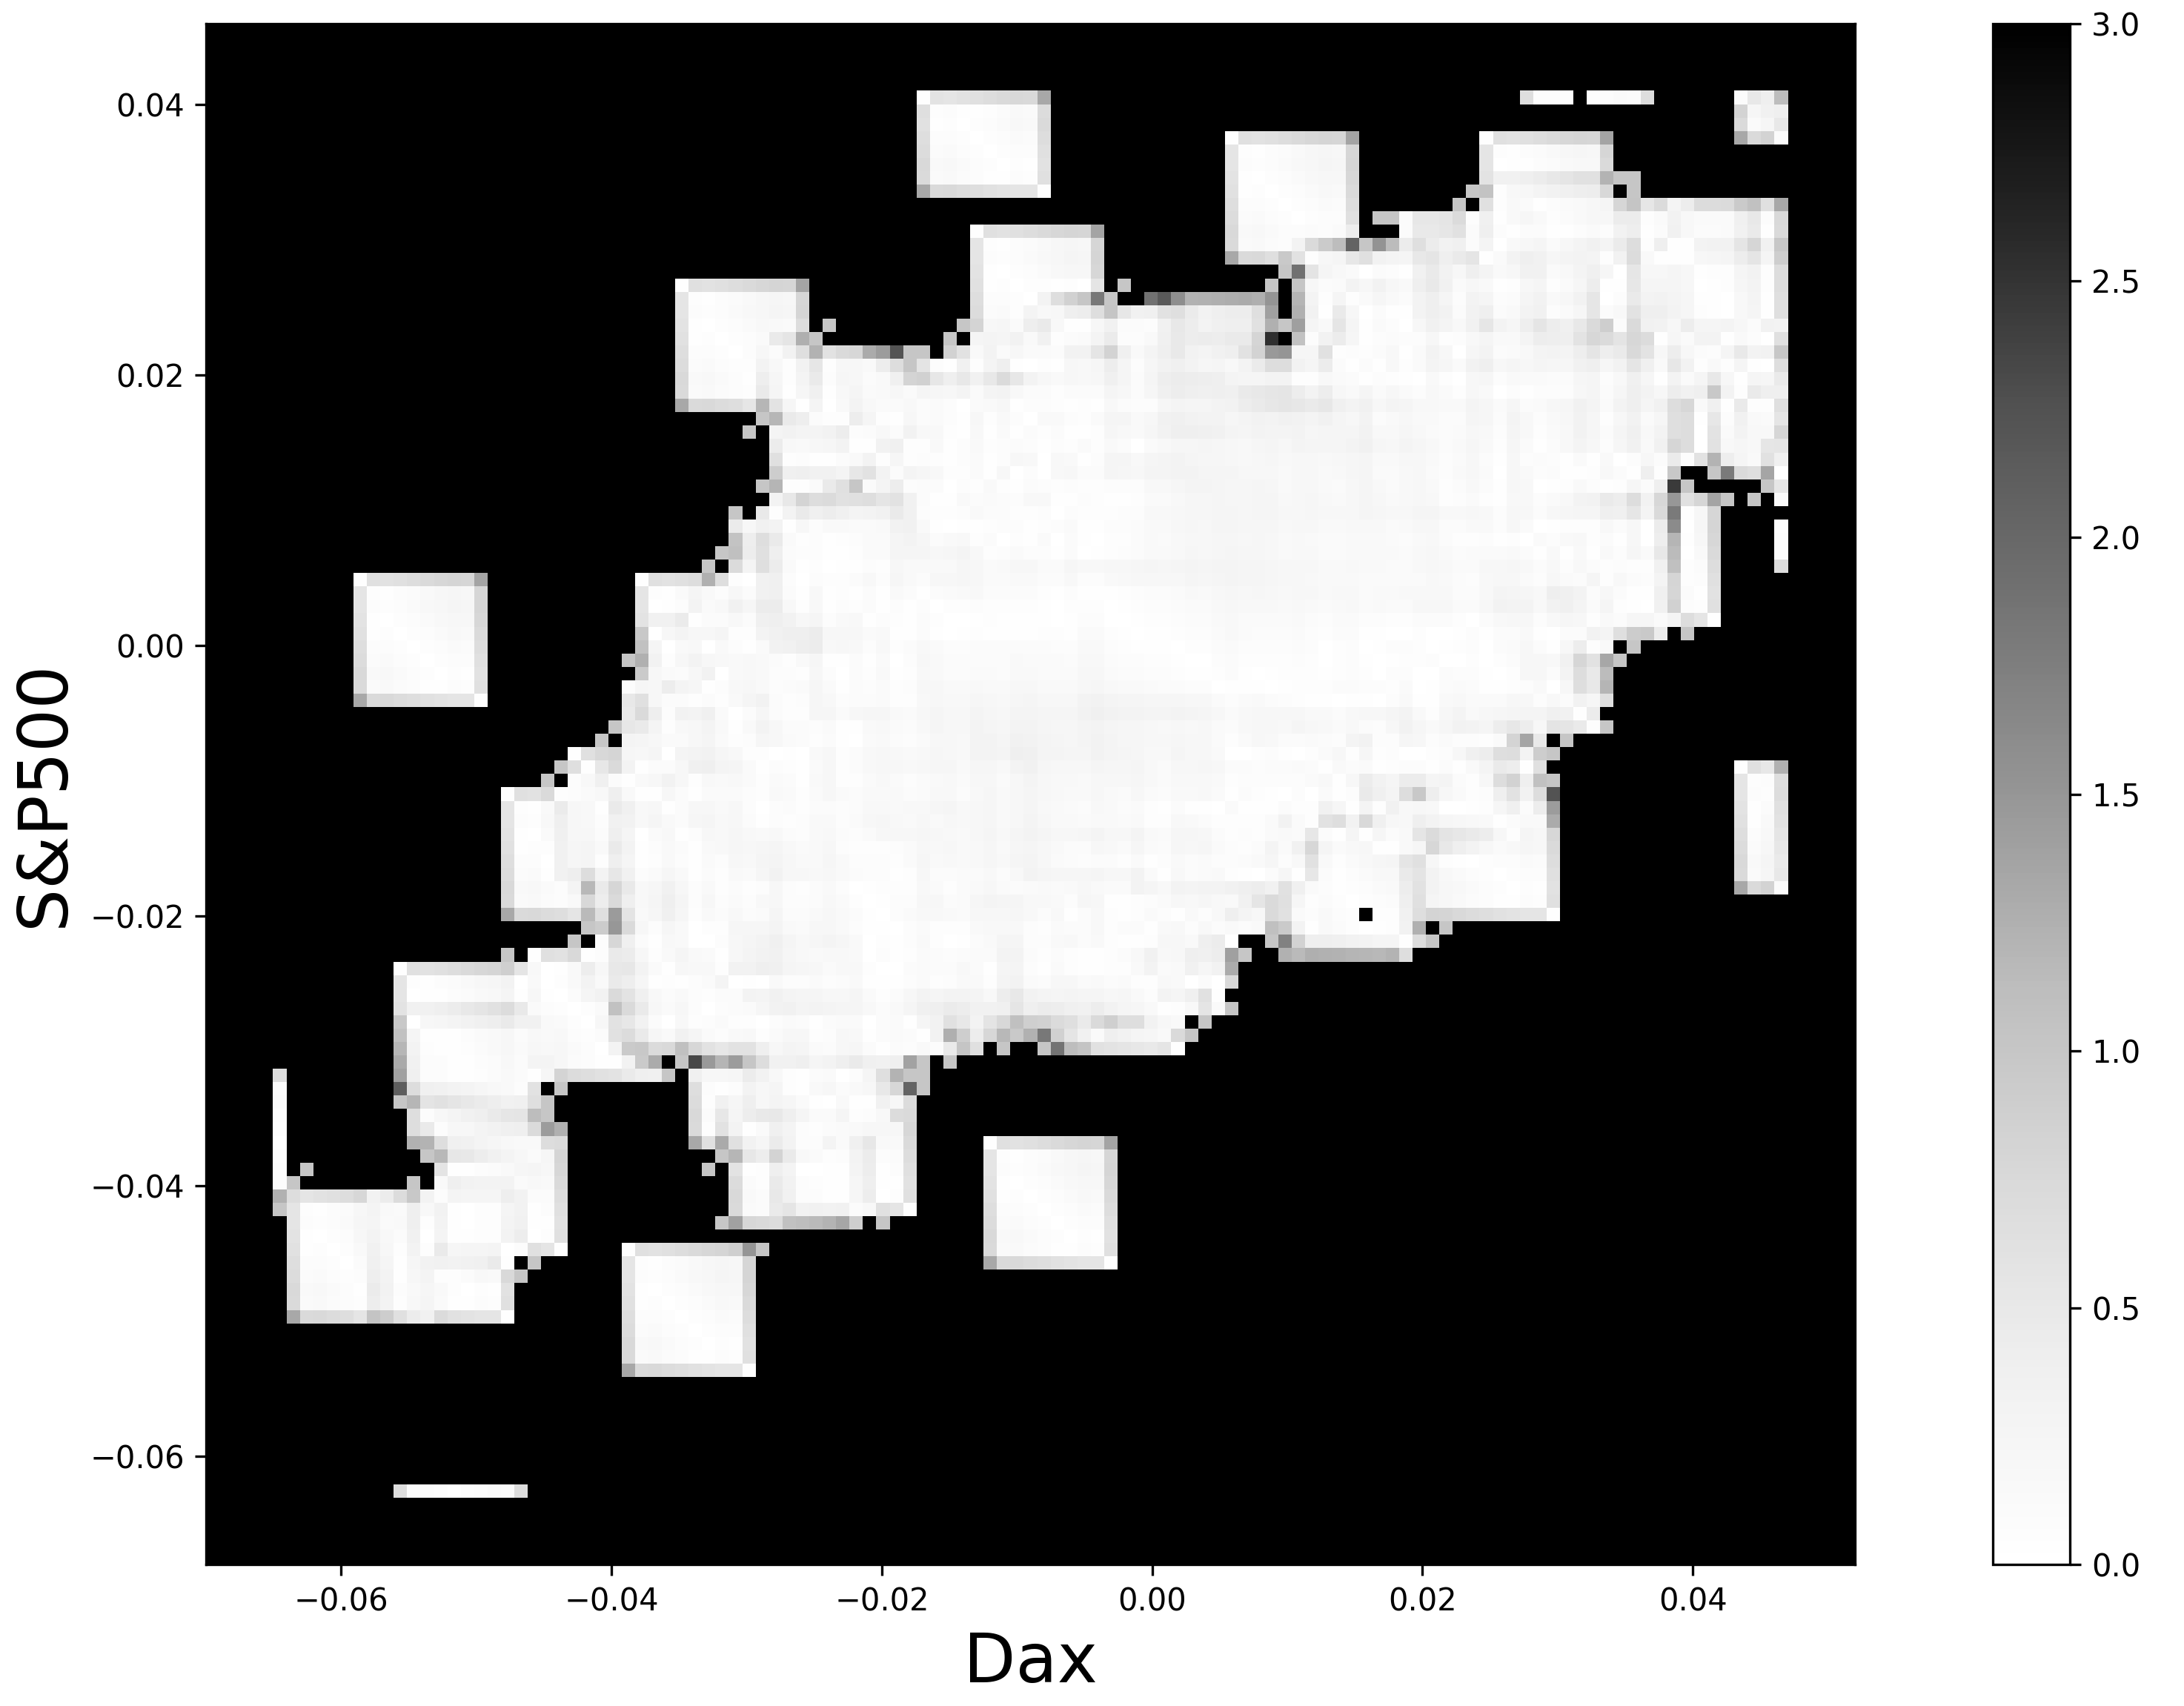
\includegraphics[width=\textwidth]{/home/hossein4527/MEGA/MEGAsync/Commit/University-Projects/MSc_Thesis/plots/Dax_SnP.png}
	\caption{پتانسیل کوانتومی مشترک محاسبه شده برای بازار های نشان داده شده در مختصات.}
	\label{fig:14}
\end{figure}
به عنوان نمونه دوم پتانسیل کوانتومی مشترک برای دو بازار 
$S\&P500$
و
$DAX$
به عنوان دو بازار وابسته در شکل
\ref{fig:14}
آورده شده است.
این پتانسیل نظیر نمونه پتانسیل کشیده شده برای ضریب همبستگی
$\rho=0.5$
در مدل گاوسی مطرح شده است.
با توجه به شکل می توان دریافت که شکل تقارن دایروی خود را از دست داده و تمایل به شکلی بیضوی پیدا کرده است. 
نکته ی مهم دیگری که می توان به آن اشاره کرد، عریض تر بودن دیواره های این پتانسیل در راستای مختصات بازار 
$DAX$
نسبت به بازار 
$S\&P500$
است و هرچه این دیواره عریض تر امکان سود دهی بیشتری فراهم خواهد بود. 

ج) پتانسیل کوانتومی محاسبه شده برای بازارهای 
$S\&P500$
و
$Dow Jowns$
به عنوان دو بازار به شدت وابسته:

 \begin{figure}[ptb]
	\centering
	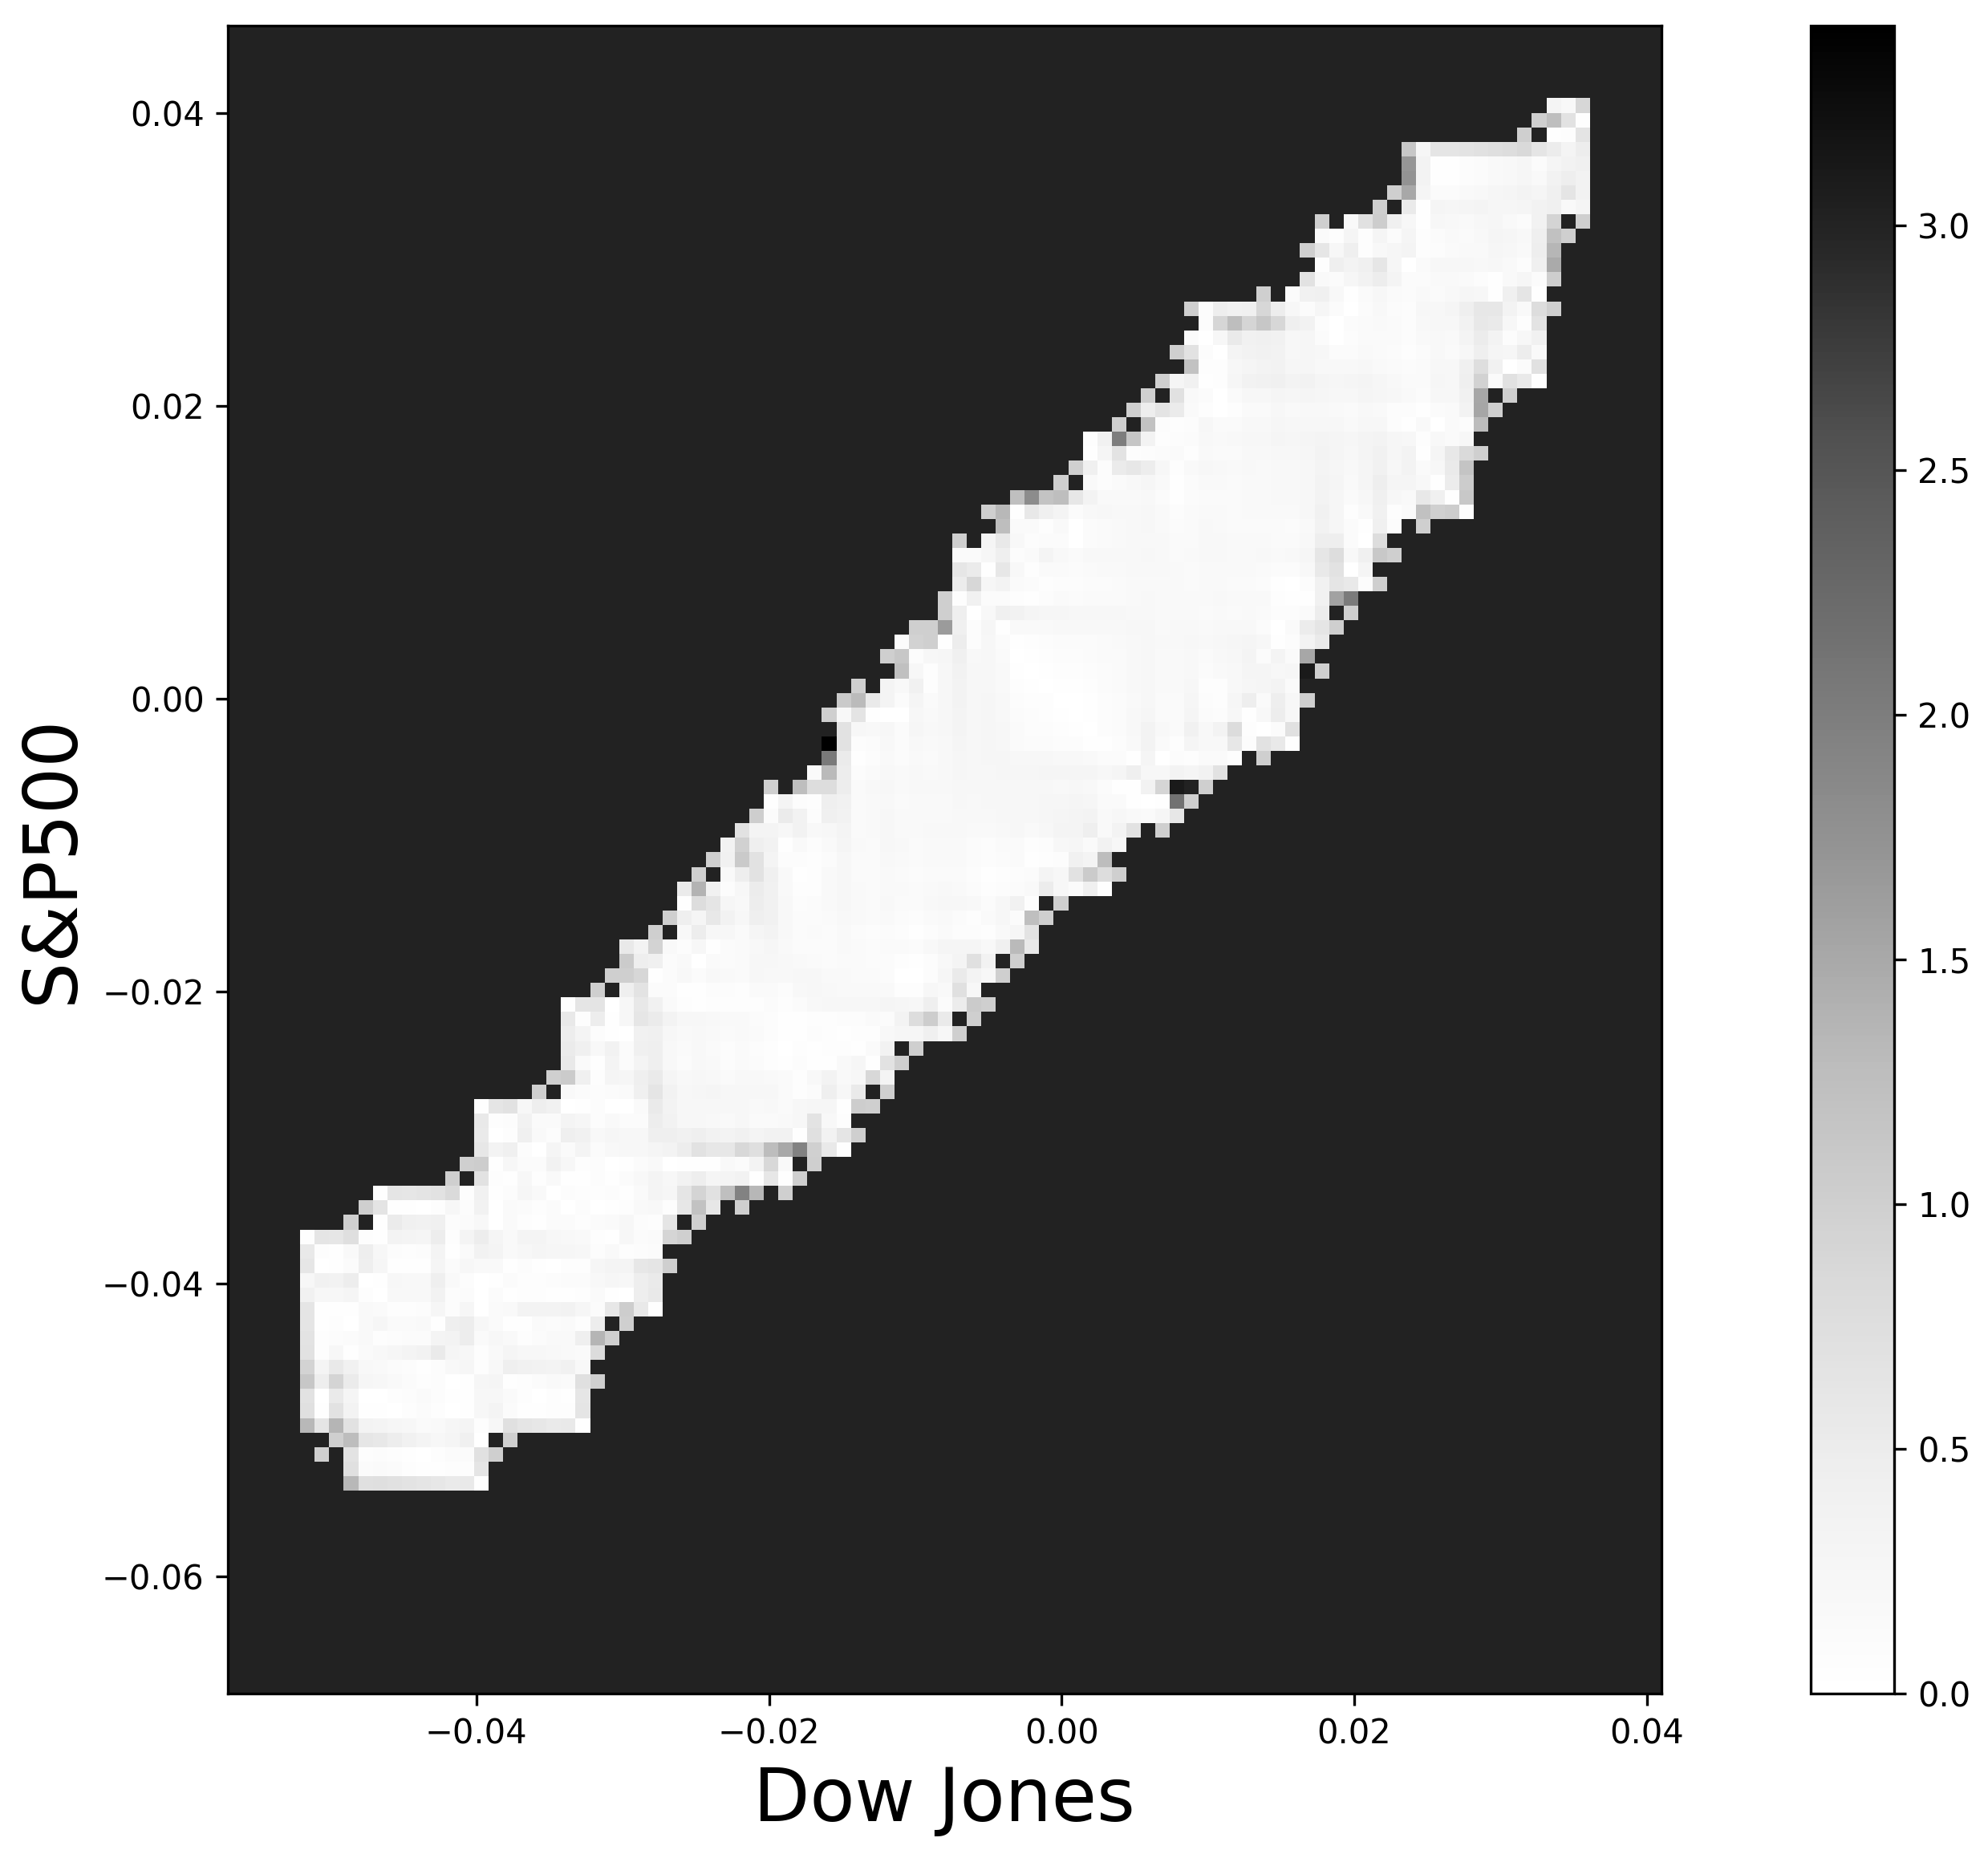
\includegraphics[width=\textwidth]{/home/hossein4527/MEGA/MEGAsync/Commit/University-Projects/MSc_Thesis/plots/Dow_SnP.png}
	\caption{پتانسیل کوانتومی مشترک محاسبه شده برای بازار های نشان داده شده در مختصات.}
	\label{fig:15}
\end{figure}
به عنوان نمونه آخر به بررسی پتانسیل کوانتومی مشترک محاسبه شده برای دو بازار 
$S\&P500$
و
$Dow Jowns$
می پردازیم. پتانسیل کوانتومی مربوطه در شکل
\ref{fig:15}
نشان داده شده است. هم با مقایسه با مدل گاوسی مطرح شده و هم با مقایسه با شکل
\ref{fig:12}
می توان نتیجه گرفت که ضریب همبستگی بین این دو بازار بشدت زیاد بوده و به همین دلیل این دو بازار در گروه بازار های به شدت وابسته قرار می گیرد.

\section{جمع بندی فصل سوم}
در این فصل با مطرح کردن یک مدل ریاضیاتی از قلب مکانیک کوانتومی بوهمی و استفاده از آن برای تحلیل و بررسی داده های تجربی بازار های مختلف دیدیم که چگونه می توان مفاهیم مکانیک آماری را توسط مکانیک کوانتومی پیاده سازی کرد. در ابتدای فصل نشان دادیم که چگونه می توان پتانسیل کوانتومی یک بعدی را برای یک بازار ترسیم کرد و در مورد مشکلات مربوطه در زمینه مدل سازی برنامه نویسی آن بحث شد. در ادامه به تعمیم این پتانسیل کوانتومی برای دو بازار پرداختیم و با ارائه مدلی گاوسی نشان دادیم که پتانسیل کوانتومی مشترک محاسبه شده برای هر دو بازار دلخواه حاوی چگونه اطلاعاتی است و برای بیرون کشیدن این اطلاعات چگونه می بایست عمل کرد. در انتها با ترسیم سه پتانسیل کوانتومی دو بعدی مشترک محاسبه شده برای شاخص های متفاوت، به بررسی میزان وابستگی بین هر یک از آن دو بازار ها پرداختیم و نشان دادیم که در میان بازارهای 
$S\&P500$،
$Dow Jones$،
$DAX$،
و
$TOPIX$،
 بازارهای 
 $S\&P500$
 و 
 $Dow Jones$
 دارای بیشترین وابستگی  و بازارهای 
 $DAX$
 و
 $TOPIX$
 دارای کمترین وابستگی هستند. 
 
 
 تا اینجای کار ما به تحلیل دیداری شکل های کشیده شده بسنده کردیم در حالی که مسیر برای محاسبات کمی در این راستا هموار است. با تحلیل های ثانویه روی شکل ها و داده های موجود می توان میزان این همبستگی را نیز محاسبه کرد و مقایسه ساده ای با اطلاعات مشابه بدست آمده از مکانیک آماری انجام داد. امید بر این است که خواننده های این پایان نامه قدم در مسیر تحقق این سوال برداشته و به یاد داشته باشد که این قدم ها هرچه اندک در راستای این سوال های موجود در کامل شدن پازل نهایی علوم اجتماعی کوانتومی نقش مهمی خواهند داشت.
 
\newpage
%==============================================================================================================================================================================================================================================================================================================================================================================================================================================
\chapter{مدیریت ریسک و  سبد سهام با استفاده از پتانسیل کوانتومی}
\section{مقدمه ای بر مدیریت ریسک و سبد سهام}
سال ۲۰۰۸، روزهایی که بازار سهام در حال ریزش شدید بود، یک صندوق سرمایه گذاری در حال جمع کردن پول و خرید اوراق بهادار با سرعت بسیار زیاد بود. این صندوق طی ۱۵هفته متوالی اوراقی به ارزش ۱۰ میلیارد دلار خریداری کرد، اوراقی که همه از آن ها فراری بودند. گویا گردانندگان این سهام جمله معروفی از جان تمپلتون را شعار خود قرار داده بودند که میگوید: "وقتی در بازار خون راه می افتد وقت خریدن است."
این صندوق که بعدها مشخص شد سود کلانی از این معاملات برده است، گرداننده ای به نام هاوارد مارکس داشت. هاوارد مارکس به نوشتن درباره ی مفهوم ریسک و بررسی آن از جنبه ها و جهات متعدد مشهور است و به قول خودش مهم ترین نکته در سرمایه گذاری ریسک است.  تعریف گفتاری ریسک به این صورت است که اتفاقات محدودی رخ خواهد داد ولی امکان رخداد تعداد بسیار زیادتری از آن اتفاقات وجود دارد. فرار از ریسک در سرمایه گذاری از آن جایی ممکن نیست که هیچ کس یا علمی نمیتواند با قاطعیت آینده را پیش بینی کند. یافتن دارایی هایی که ارزش آن ها در آینده احتمالن بالا خواهد رفت کار سختی نیست و خرید تعداد کافی از این دارایی ها احتمالن به سود منجر خواهد شد. اما اگر ریسک خریدن این دارایی ها را در نظر نگرفته باشیم، در بلند مدت ضرر خواهیم کرد.   در مسیر خرید هر دارایی به امید سود کردن مراحلی نیاز است طی شود که اولین آن شناخت ریسک های مربوط به آن دارایی است. قدم دوم شناخت دینامیک ریسک مورد نظر است، یعنی بتوانیم تشخیص دهیم که این ریسک چه زمان هایی زیاد و چه زمان هایی کم می شود. قدم آخر برای هر سرمایه گذاری نحوه کنترل ریسک های موجود را شامل می شود. 

اهمیت شناخت ریسک در آن جاییست که اولا انسان ذاتی ریسک گریز دارد و از عدم اطمینان و عدم قطعیت خوشش نمی آید و دوما میزان سود و ضرر از خرید یا فروش هر دارایی رابطه ای مستقیم با میزان ریسک موجود در آن دارایی دارد. برای مثال دو دارایی مختلف را در نظر بگیریم که سرمایه گذاری در آن ها سودی یکسان خواهد داشت ولی ریسک متفاوتی دارند، بدیهی است که سرمایه گذاران در درجه اول آن دارایی ای را انتخاب می کنند که ریسک کمتری دارد. اگر در ابتدا قیمت این دو دارایی برابر باشد، تمایل سرمایه گذاران به خرید دارایی کم ریسک تر قمتش را بالا می برد و در نتیحه آن به فرض ثابت بودن سود، بازدهی سرمایه گذاری پایین می آید. این وضعیت در مورد دارایی پر ریسک تر برعکس عمل می کند و عدم تمایل سرمایه گذار به خرید دارایی به علت ریسک زیاد موجود در آن، قیمت دارایی را کمتر و کمتر می کند و به فرض ثابت بودن سود،  بازدهی سرمایه گذاری در آن بالا می رود و خرید آن را کمی جذاب تر می کند.  این مثال مکانیسم بازار برای ایجاد تعادل بین بازدهی و ریسک است. 

در نظریه مدیریت مالی جدید، ریسک برابر تلاطم یا واریانس در نظر گرفته می شود و برای مثال هر قدر قیمت دارایی در بازار ملاطم تر باشد، ریسک بالاتری خواهد داشت. در همین ابتدای تعریف ریسک نظر افرادی چون وارن بافت و هاوارد مارکس با نظریه پردازها که ریسک را تلاطم قیمت میدانند متفاوت است. در دیدگاه این افراد ریسک برابر تلاطم قیمت نیست بلکه برابر تلاطم ارزش ذاتی دارایی است. قیمت حاصل کشمکش ها و برهمکنش های فعالان بازار است، بازاری که می تواند همیشه کارامد نباشد و گاهی فعالان بازار همانطور که دیدیم تخمین درستی از ارزش دارایی ها ندارند. گاهی اوقات نیز عدم توافق فعالان بازار بر روی ارزش دارایی نیز باعث زیاد شدن تلاطم در قیمت آن داراریی و به طبع آن زیاد شدن ریسک منجر می شود که این موضوع در نظر افراد ارزش نگری چون وارن بافت تعریفی درست از ریسک را دارا نمی باشد. در نگاه این افراد ریسک به معنای احتمال از دست رفتن دائمی سرمایه است. در حقیقت هیچ کدام از این نگرش ها به تنهایی تعریفی جامع و کامل از ریسک نیستند و از نظر دیدگاه اینجانبان ریسک موضوعی شخصی است و برای هر معامله مقدار مشخص و متفاوتی نسبت به معامله دیگر دارد.

سرمایه گذاران در هر زمان دلخواهی حس رضایت کافی نداشته باشند می توانند پول خود را از صندوق های سرمایه گذاری بیرون بکشند. همین امر باعث می شود که مدیران صندوق های سرمایه گذاری دیدگاهی کوتاه مدت نسبت به ریسک داشته باشند و برای راضی نگه داشتن سرمایه گذاران  تلاطم های قیمت در بازه های کوتاه مدت را در خرید و فروش های خود در نظر بگیرند.  به بیان خلاصه تر هرچه افق سرمایه گذاری کوتاه تر شود، به تعریف نظریه پردازها از ریسک نزدیکتر می شویم. برای بهتر متوجه شدن این موضوع بهتر است آن را در داده های واقعی نمایش دهیم.

\subsection{واریانس تعریفی دانشگاهی از ریسک}
نمودار داده های قیمتی شاخص
$S\&P500$
برای سال های بین ۲۰۰۰ تا ۲۰۰۵ در شکل 
\ref{fig:5.1}
 رسم شده است.
\begin{figure}[ptb]
	\centering
	\includegraphics[width=\textwidth]{/home/hossein4527/MEGA/MEGAsync/Commit/University-Projects/MSc_Thesis/plots/fig1.png}
	\caption{سری زمانی قیمت شاخص S\&P500}
	\label{fig:5.1}
\end{figure}
اگر بخواهیم تعریف ریسک به عنوان تلاطم قیمت را برای این داده ها به صورت روزانه نشان دهیم باید واریانس سری زمانی قیمت آن را رسم کنیم. شکل
\ref{fig:5.2}
میانگین واریانس سری زمانی شکل 
\ref{fig:5.1}
را برای سرمایه گذاری با افق دید ۲ تا ۶۰۰ روزه را نشان می دهد. 
\begin{figure}[ptb]
	\centering
	\includegraphics[width=\textwidth]{/home/hossein4527/MEGA/MEGAsync/Commit/University-Projects/MSc_Thesis/plots/fig5_2.png}
	\caption{سری زمانی قیمت شاخص S\&P500}
	\label{fig:5.2}
\end{figure}
با توجه به شکل
\ref{fig:5.2}
به وضوح مشخص است که هر چه مدت  سرمایه گذاری در این شاخص طی سال های ۲۰۰۰ تا ۲۰۰۵ بیشتر شده است، ریسک موجود در این سرمایه گذاری افزایش یافته است.  این همان تعریف نظریه پردازها از ریسک موجود در یک سری زمانی است. در این قسمت از پایان  نامه میخواهیم نشان دهیم  که آیا می توان تعریف کمی دیگری را در کنار واریانس برای ریسک تعریف کرد و آیا با کنترل کردن پتانسیل کوانتومی می توان برای یک سری زمانی ریسک تعریف کرد و از آن برای مقایسه با تعاریف دیگر ریسک کمک گرفت. از اینجا به بعد به نحوه محاسبه ریسک با کمک پتانسیل کوانتومی میپردازیم.
\section{مدیریت ریسک و سبد سهام توسط پتانسیل کوانتومی}
در فصل سوم نشان دادیم که چگونه می توان پتانسیل کوانتومی یک بعدی حاکم بر سود و زیان یک بازار را محاسبه کرد. در ادامه این فصل میخواهیم با در نظر گرفتن فاصله ی بین دو دیواره مشخص شده در شکل
\ref{fig:5.3}
تحت عنوان ریسک موجود در آن بازار به بررسی ریسک موجود در بازار های مختلف بپردازیم و با مقایسه آن با واریانس تحت عنوان ریسک کلاسیکی به تشکیل سبد سهام مناسب بپردازیم. 
\begin{figure}[ptb]
	\centering
	\includegraphics[width=\textwidth]{/home/hossein4527/MEGA/MEGAsync/Commit/University-Projects/MSc_Thesis/plots/fig5_4.png}
	\caption{پتانسیل کوانتومی حاکم بر داده های روزانه بازار S\&P500}
	\label{fig:5.3}
\end{figure}
واژه مناسب در دیدگاه افراد و صندوق های سرمایه گذاری مختلف، متفاوت است و هرکدام از آن ها بسته به نوع هدف سرمایه گذاری دنبال جنبه ای متفاوت از سود هستند. در کار این پایان نامه سبدی را مناسب میبینیم که دارای کمترین ریسک ممکن در بین تمامی سبد های ممکن باشد و همچنین در بین تمامی سبد های با ریسک کمینه، حاوی سود بیشینه باشد.  برای این کار ابتدا لازم است که نموداری شماتیک از نحوه ایجاد سبد سهام با در نظر گرفتن ریسک هر کدام را داشته باشیم.  شکل 
\ref{fig:5.4}
به صورت کلی تشکیل سبد سهام از هر تعداد دلخواه سری زمانی قیمتی را نشان می دهد. 
\begin{figure}[ptb]
	\centering
	\includegraphics[width=\textwidth]{/home/hossein4527/MEGA/MEGAsync/Commit/University-Projects/MSc_Thesis/plots/new1_fig0.png}
	\caption{شکل شماتیک نحوه تشکیل شاخص سبد سهام با وزن های مختلف}
	\label{fig:5.4}
\end{figure}

برای هر تعداد دلخواه سهم می توان سبدی با وزن های مربوطه تشکیل داد که شاخص سود و زیان این سبد از معادله زیر بدست می آید.
\begin{equation}
\bar{r}(t)=\sum_{i=1}^{N} w _{i}r_{i}(t)،
\label{eq:3}
\end{equation}
  
 که در آن
$W_i$
ها وزن های هر کدام از سهام های در نظر گرفته در سبد مورد نظر  هستند. در ادامه کار با استفاده از الگوریتم ژنتیک تلاش در جهت یافتن وزن های مناسبی خواهیم کرد که سبد نهایی متشکل از این وزن ها دارای کمترین ریسک ممکن در بین تمامی گزینه های موجود باشند. 
الگوریتم ژنتیک الگوریتمی محبوب در میان کد نویسان است که معمولا برای یافتن اکسترمم های توابع چند متغیره از آن استفاده می شود. در کار این پایان نامه از زبان برنامه نویسی پایتون برای پیاده سازی این الگوریتم کمک گرفته شده است. اگر این برنامه را برای سبدی متشکل از ۸ شاخص بزرگ دنیا همچون 
$Dow Jones industrial, $
$S\&P 500 composite,$
$ FTSE 100, TOPIX ,$
$DAX 30 performance,$
$ NIKKEI 225,$
$ Korea SE composite $
و
 $ Shanghai SE A$
 اجرا کنیم، فرایند کمینه شدن ریسک شاخص سبد سهام در شکل 
 \ref{fig:5.5}
 قابل مشاهده است.
\begin{figure}[ptb]
	\centering
	\includegraphics[width=\textwidth]{/home/hossein4527/MEGA/MEGAsync/Commit/University-Projects/MSc_Thesis/plots/fig6pr.png}
	\caption{شکل شماتیک }
	\label{fig:5.5}
\end{figure}
همانطور که در شکل 
\ref{fig:5.5}
پیداست، در مرحله نهایی کمینه کردن تعدادی سبد سهام با ریسک کمینه یکسان وجود دارند. این مساله چندان به دور از انتظار هم نیست چرا که سهم های مختلف کاملن از یکدیگر مستقل نیستند و تعداد بیشماری حالت برای کمینه ریسک در بین تمامی حالات ممکن موجود است. پنج حالت ممکن برای برنامه اجرا شده در شکل 
\ref{fig:5.5}
نشان داده شده اند. به وضوح در این شکل شماتیک پیداست که این سبد ها با یکدیگر متفاوت بوده در حالی که همه آن ها متعلق به یک گروه از سبد ها با ریسک یکسان هستند.  هر کدام از این پنج سبد مشخص شده در شکل
\ref{fig:5.5}
از نقطه نظر ریسک کوانتومی با یکدیگر برابر بوده و اگر تنها همین پارامتر در خرید دارایی هائز اهمیت بود هیچ کدام از این پنچ سبد بر دیگری ارجحیت خاصی نداشتند. این در حالی است که برای انتخاب سبد تعداد بیشماری پارامتر وجود دارد که می توان از آن ها برای فیلتر کردن سبدهای موجود استفاده کرد. سوال خوبی که می توان در این قسمت پرسید این است که ترتیب اعمال فیلتر ها اهمیت خاصی دارد یا خیر؟ یعنی اگر در ابتدا سبدهای پر بازده را جدا کرده و از بین آن ها دنبال سبدهای کم ریسک گشت نتیجه یکسانی با انتخاب ابتدا سبدهای کم ریسک و سپس پر بازده دارد یا خیر؟ پاسخ دادن به این سوال ورای کار این پایان نامه قرار دارد و خواننده می تواند به راحتی به دنبال پاسخ این سوالات بگردد.

شکل 
\ref{fig:5.6}
ریسک و واریانس هر کدام از شاخص های استفاده شده در برنامه الگریتم ژنتیک را در کنار ریسک و واریانس سبد متشکل از این شاخص ها با وزن های پیدا شده در این الگریتم را نشان می دهد. 
هر کدام از ریسک های بدست آمده تقسیم بر ریسک شاخص شانگهای که بزرگترین ریسک  موجود در بین دیگر شاخص ها را دارد، شده است. به این ترتیب ریسک های نمایش داده شده مقیاسی بوده و مقایسه بین هر کدام از آن ها ساده تر انجام خواهد شد. با مشاهده در شکل 
\ref{fig:5.6}
در می یابیم که شاخص های داو جونز و اس اند پی آمریکا کمترین ریسک و شاخص شانگهای چین بیشترین ریسک را در بین هر یک از هشت شاخص دیگر دارد. این در حالی است که سبد سهام متشکل از تک تک این شاخص ها با وزن های مناسب پیدا شده در الگوریتم ژنتیک برنامه، ریسکی کمتر از حتی شاخص های داو جونز و اس اند پی دارد. با تفکری سطحی می توان پی برد که ریسک سبد تابعی خطی از ریسک اجزا تشکیل دهنده آن سبد نیست و اگر چنان بود، ریسک سبد در کمترین حالت خود زمانی بود که سبد متشکل از صد در صد سهم داو جونز بود و ریسک آن برابر ریسک شاخض داو جونز قرار می گرفت. در حالی که این اتفاق مطابق با شکل
\ref{fig:5.6}
رخ نداده است.

برای مقایسه بهتر واریانس که نماینده ریسک در بین نظریه پردازان است هم در کنار ریسک کوانتومی خارج شده از پتانسیل کوانتومی رسم شده است.  همانطور که پیداست در اکثر شاخص های رسم شده واریانس مقداری کمتر از ریسک کوانتومی اختیار کرده است و تنها در مورد سبد نهایی این مقدار متفاوت نمایان شده است. 
 
\begin{figure}[ptb]
	\centering
	\includegraphics[width=\textwidth]{/home/hossein4527/MEGA/MEGAsync/Commit/University-Projects/MSc_Thesis/plots/fig5_6.png}
	\caption{پتانسیل کوانتومی حاکم بر داده های روزانه بازار S\&P500}
	\label{fig:5.6}
\end{figure}
\section{تضاد ریسک با  بازدهی}
در ابتدای فصل نشان دادیم که چگونه بازار تعادل بین ریسک و بازدهی را نگه می دارد. در این بخش می خواهیم نشان دهیم که این تعادل در بین سبد های پیشنهادی الگوریتم ژنتیک چگونه بر قرار است و آیا می توان در بین تعداد بیشمار تبگهی موجود پیشنهادی این برنامه، تفکیک از نقطه نظر میزان بازدهی کرد. برای این کار یکی از بهترین کار های ممکن این است که سبد های پیشنهادی برنامه الگوریتم ژنتیک را تشکیل دهیم و با استفاده از داده های تاریخی میزان بازدهی کل این سبد را در بازه مشخص بسنجیم. برای این کار بار دیگر برنامه الگوریتم ژنتیک را اجرا می کنیم و این بار تعداد ۹ عدد سبد هم ریسک را از بین سبد های با تبهگنی یکسان جدا میکنیم. این نه سبد در شکل 
\ref{fig:5.7} 
آورده شده ایند.
\begin{figure}[ptb]
	\centering
	\includegraphics[width=\textwidth]{/home/hossein4527/MEGA/MEGAsync/Commit/University-Projects/MSc_Thesis/plots/fig20.png}
	\caption{سبدهای سهام پیشنهادی الگوریتم ژنتیک}
	\label{fig:5.7}
\end{figure}
برای هر کدام از این سبد ها بازدهی محاسبه شده در شکل
\ref{fig:5.8}
آورده شده است. با توجه در این شکل می توان نتیجه ابتدایی گرفت که سبد نهم از بین سبد های نشان داده شده بازدهی بیشتری نسبت به دیگر سبد ها را به خود اختصاص داده است. این در حالی است که سبد دوم در میدان رقابت با دیگر سبدها شکست خورده است. 
\begin{figure}[ptb]
	\centering
	\includegraphics[width=\textwidth]{/home/hossein4527/MEGA/MEGAsync/Commit/University-Projects/MSc_Thesis/plots/fig10.png}
	\caption{بازدهی هر کدام از سبدهای پیشنهادی شکل \ref{fig:5.7}}
	\label{fig:5.8}
\end{figure}
در این فصل نشان دادیم که چگونه می توان با استفاده از فیلتر های مختلف سبد سهام دلخواه خود را پیدا کرد و در این مسیر از فیلتر های کوانتومی برای جداسازی سبدهای سهام کمک گرفتیم. همانطور که در پیشگفتار گفته شد هدف اولیه برای اثبات درستی استفاده از مکانیک کوانتومی در تحلیل بازارهای مالی مقایسه تمامی فیلترهای آن با فیلتر های استاندارد موجود، در اینحا واریانس تحت عنوان ریسک استاندارد است. 
برای مقایسه ریسک کوانتومی و ریسک استاندارد واریانس بهتر است به مقایسه این دو در سری های زمانی با مقیاس های متفاوت بپردازیم.
برای این مقایسه کافی است یک سبد پیشنهادی الگوریتم ژنتیک را برای مقیاس های یک روز، دو روز الی دویست روز تشکیل دهیم. شکل 
\ref{fig:5.9}
مقدار ریسک کوانتومی و ریسک استاندارد را برای هر کدام از این مقیاس ها نشان می دهد. همانطور که در این شکل پیداست در بازه های زمانی دو روزه خرید و فروش از نقطه نظر ریسک استاندارد ریسک بزرگتری از نقطه نظر ریسک کوانتومی دارد ولی از بازه های دو روز به بعد ریسک کوانتومی مقدار ریسک کمتری را نشان می دهد. از شکل 
\ref{fig:5.9}
مشخص است که یک رابطه نمایی بین مقیاس و ریسک وجود دارد. این رابطه از معادله زیر با نماهای مربوطه نشان داده شده در شکل پیروی می کند. 
\begin{equation}
Risk(\tau) \propto \tau^\alpha.
\label{eq:4}
\end{equation}
\begin{figure}[ptb]
	\centering
	\includegraphics[width=\textwidth]{/home/hossein4527/MEGA/MEGAsync/Commit/University-Projects/MSc_Thesis/plots/fig3_a.png}
	\caption{رابطه نمایی ریسک با مقیاس}
	\label{fig:5.9}
\end{figure}
همانطور که در شکل
\ref{fig:5.9}
به وضوح پیداست نمای بحرانی برای ریسک استاندارد بزرگ تر از نمای بحرانی برای ریسک کوانتومی است و این بیان  گر این موضوع است که ریسک کوانتومی نسبت به ریسک استاندارد آینده بهتری را برای این سبد پیش بینی می کند.

\section{جمع بندی فصل چهارم}
در این فصل با استفاده از کنترل پتانسیل کوانتومی معیاری برای ریسک سری های زمانی تعریف کردیم و نشان دادیم که این معیار در مقایسه با معیار کلاسیکی خود که واریانس است چگونه عمل می کند. در ادامه به بررسی مدیریت سبد سهام با هدف یافتن سبدی که دارای کمترین ریسک در بین تمامی انتخاب های ممکن است، سبد هایی را معرفی کردیم که در کمینه ریسک قرار داشتند و تبهگن بودند. از نقطه نظر کمترین ریسک هیچ اولویتی بین این سبد ها وجود نداشت ولی از نقطه نظر میزان بازدهی، تفاوت هایی در بین آن ها مشاهده شد. در نهایت نشان دادیم که چگونه می توانیم این تفاوت ها را نمایان کنیم و در مسیر انتخاب بهترین سبد ممکن از نقطه نظر کمترین ریسک و بیشترین بازدهی حرکت کنیم.


%==============================================================================================================================================================================================================================================================================================================================================================================================================================================


\chapter{نتیجه گیری و پیشنهادات}
در این پایان نامه از ابتدا صحبت از آن بود که چگونه ابزارهای مستقل ریاضیاتی که برای پاسخگویی به مسائلی خاص از علم به وجو آمده اند می توانند پاسخگو در دیگر زمینه های زندگی بشر نیز باشند. یکی از این ابزار ها مکانیک کوانتومی است که برای پاسخ گویی به سوالات موجود در میکروسیستم های فیزیکی تولد یافته است. 

در فصل اول سخن از این به میان آمد که آیا مکانیک کوانتومی توانایی یافتن پاسخ نیازهای بشر ورای مسائل مربوط به اتم و موضوعات وابسته را دارد؟ اگر دارد کدامین جنبه از مشکلات آدمیان را می تواند تحلیل کند و جواب های آن تا چه حد قابل مقایسه با دیگر ابزارهای موجود است؟ آیا مکانیک کوانتومی اراده قدم گذاشتن در مسیر حل مشکلاتی(همچون مشکلات فرایند شناختی، تحلیل روانشناسی بازار و غیره) که ابزارهای موازی با آن تاب نفس کشیدن در آن ها را ندارند، دارد؟ 

برای یافتن این چنین سوالات فصولی را مرتب کردیم که مقدمه ای بر تحکیم جنبش علوم اجتماعی کوانتومی هستند. از جمله این فصول، فصل سوم این پایان نامه، تعمیم پتانسیل کوانتومی در مطالعه بازارهای همبسته و فصل چهارم مدیریت ریسک و سبد سهام به کمک پتانسیل کوانتومی هستند.

در فصل سوم با ارائه مدلی پیشنهادی برای تابع توزیع سود و ضرر یک بازار، رفتار پتانسیل کوانتومی مشترک را در موقعیت های متفاوت ترسیم کردیم. نشان دادیم که پتانسیل کوانتومی مشترک برای بازار های با وابستگی زیاد چگونه نسبت به بازارهای با وابستگی کم تغییر می کند. همچنین برای داده های واقعی بازارهای مختلف از سراسر دنیا این پتانسیل را ترسیم کردیم و در ادامه تحلیل آنها دریافتیم که پتانسیل کوانتومی مشترک همانند ابزارهای کلاسیکی موجود به خوبی از وجود همبستگی بالا میان شاخص های 
$S\&P500$
و 
$Dow Jones$
و همچنین از وجود همبستگی کم میان بازارهای 
$DAX$
و 
$TOPIX$
جکایت می کند. 

نباید این گونه برداشت کرد که اطلاعات خروجی از پتانسیل کوانتومی همان اطلاعات موجود در تابع همبستگی مکانیک آماری است و چیزی جدید به دانسته های قبلی ما اضافه نکرده است. می بایست حواسمان باشد همانگونه که فضا و چارچوب این دو ابزار(مکانیک کوانتومی و مکانیک آماری) به کلی متفاوت از یکدیگر بوده، میزان اطلاعات خروجی از هر کدام از این دو ابزار به کلی با یکدیگر متفاوت است.  یادمان باشد که هدف در این قسمت نشان دادن این موضوع بود که مکانیک کوانتومی هم همانند برادر بزرگتر خود مکانیک آماری می تواند پاسخگو در مسائل موجود باشد. 

در ادامه در فصل چهارم نیز با کمک پتانسیل کوانتومی حاکم بر یک بازار نشان دادیم که چگونه شکل پتانسیل کوانتومی می تواند منعکس کننده ریسک موجود در آن بازار برای سرمایه گذاری باشد و با مقایسه این ابزار با تابع واریانس موجود در مکانیک آماری شباهت ها و تفاوت های موجود در این دو مفهوم را بررسی کردیم. از جمله تفاوت های قابل بحث در این حوزه بیشتر بودن ریسک پتانسیل کوانتومی یک بازار نسبت به واریانس آن بازار است در حالی که سبد ساخته شده با در نظر گرفتن پتانسیل کوانتومی ریسک کمتری در بلند مدت نسبت به واریانس داشته است. 

بررسی این دو کار در این پایان نامه نمونه کوچکی از کارهای قابل اجرا برای نشان دادن قدرت مکانیک کوانتومی در یافتن جواب مشکلات جدید جوامع امروزی است. اولین و مهمترین قدم برای مستحکم تر کردن این مفهوم استفاده از مدل های غیر گاوسی در مدل پیشنهادی برای تاع توزیع سود و زیان بازارهاست. غیر گاوسی بودن بازارها در کارهای مقاله های مختلف بررسی شده است و خوب است که دانشجوهای مشتاق در ابتدا به بررسی مدل های غیر گاوسی در تابع توزیع به کار رفته در پتانسیل کوانتومی بپردازند.
 

%######################################################################################################################################################################################################################################################################################################
\begin{thebibliography}{99}

\begin{LTRitems}
	\bibitem{black}
	Black, Fischer, and Myron Scholes. "The pricing of options and corporate liabilities." Journal of political economy 81.3 (1973): 637-654.
\end{LTRitems}	
	
\begin{LTRitems}
\bibitem{bac}
Bachelier, L. (1900). Théorie de la spéculation. Annales scientifiques de l’Ecole
Normale Supérieure, 21–86.
\end{LTRitems}

\begin{LTRitems}
	\bibitem{mandel}
	Mandelbrot, Benoit B. "The variation of certain speculative prices." Fractals and scaling in finance. Springer, New York, NY, 1997. 371-418.
\end{LTRitems}

\begin{LTRitems}
	\bibitem{kada}
	Kadanoff, Leo P. "From simulation model to public policy: An examination of Forrester's" Urban Dynamics"." Simulation 16.6 (1971): 261-268.
\end{LTRitems}

\begin{LTRitems}
	\bibitem{mont}
	Montroll, Elliott W., and Wade W. Badger. Introduction to quantitative aspects of social phenomena. Gordon and Breach, 1974.
\end{LTRitems}

\begin{LTRitems}
	\bibitem{santa}
	Anderson, P. W., and K. J. Arrow. "D. Pines (eds.)(1988), The Economy as an Evolving Complex System, Redwood City."
\end{LTRitems}

\begin{LTRitems}
	\bibitem{penrose}
	Penrose, Roger. Shadows of the Mind. Vol. 4. Oxford: Oxford University Press, 1994.
\end{LTRitems}

\begin{LTRitems}
	\bibitem{hamrof}
	Hameroff, Stuart R. "Quantum coherence in microtubules: A neural basis for emergent consciousness?." Journal of consciousness studies 1.1 (1994): 91-118.
\end{LTRitems}

\begin{LTRitems}
	\bibitem{kh2}
	Khrennivov, Andrei. "Classical and quantum mechanics on information spaces with applications to cognitive, psychological, social, and anomalous phenomena." Foundations of Physics 29.7 (1999): 1065-1098.
\end{LTRitems}

\begin{LTRitems}
	\bibitem{kh3}
	Khrennikov, A. Yu. "Information Dynamics in Cognitive, Psychological." Social and Anomalous Phenomena. Kluwer (2004).
\end{LTRitems}

\begin{LTRitems}
	\bibitem{gold}
	Goldstein, Sheldon. "Bohmian mechanics and quantum information." Foundations of Physics 40.4 (2010): 335-355.
\end{LTRitems}

\begin{LTRitems}
	\bibitem{boosem}
	Bouwmeester, Dirk, and Anton Zeilinger. "The physics of quantum information: basic concepts." The physics of quantum information. Springer, Berlin, Heidelberg, 2000. 1-14.
\end{LTRitems}

\begin{LTRitems}
	\bibitem{fucks}
	Fuchs, Christopher A. "Quantum mechanics as quantum information (and only a little more)." arXiv preprint quant-ph/0205039 (2002).
\end{LTRitems}

\begin{LTRitems}
	\bibitem{kh1}
	Khrennikov, A. Y. "Ubiquitous Quantum Structure from Psychology to Finance. Springer." (2010).
\end{LTRitems}

\begin{LTRitems}
	\bibitem{haven1}
	Shen, C., and E. Haven. "Using empirical data to estimate potential functions in commodity markets: some initial results." International Journal of Theoretical Physics 56.12 (2017): 4092-4104.
\end{LTRitems}

\begin{LTRitems}
	\bibitem{tahmaseb}
	Tahmasebi, F., et al. "Financial market images: a practical approach owing to the secret quantum potential." EPL (Europhysics Letters) 109.3 (2015): 30001.
\end{LTRitems}

\begin{LTRitems}
	\bibitem{nas1}
	Nasiri, Sina, Eralp Bektas, and Gholamreza Jafari. "Risk Information of Stock Market Using Quantum Potential Constraints." Emerging Trends in Banking and Finance. Springer, Cham, 2018. 132-138.
\end{LTRitems}

\begin{LTRitems}
	\bibitem{nas2}
	Nasiri, Sina, Eralp Bektas, and G. Reza Jafari. "The impact of trading volume on the stock market credibility: Bohmian quantum potential approach." Physica A: Statistical Mechanics and its Applications 512 (2018): 1104-1112.
\end{LTRitems}

\begin{LTRitems}
	\bibitem{kh4}
	Khrennikov, Andrei Y. Ubiquitous quantum structure. Springer, 2014.
\end{LTRitems}

\begin{LTRitems}
	\bibitem{olg1}
	Choustova, Olga. Pilot wave quantum model for the stock market. No. quant-ph/0109122. 2001.
\end{LTRitems}

\begin{LTRitems}
	\bibitem{olg2}
	Choustova, Olga. "Bohmian mechanics for financial processes." Journal of Modern Optics 51.6-7 (2004): 1111-1111.
\end{LTRitems}

\begin{LTRitems}
	\bibitem{olg3}
	Choustova, Olga. "Price‐Dynamics of Shares and Bohmian Mechanics: Deterministic or Stochastic Model?." AIP Conference Proceedings. Vol. 889. No. 1. American Institute of Physics, 2007.
\end{LTRitems}

\begin{LTRitems}
	\bibitem{olg4}
	Choustova, Olga. "Quantum modeling of nonlinear dynamics of stock prices: Bohmian approach." Theoretical and Mathematical Physics 152.2 (2007): 1213-1222.
\end{LTRitems}

\begin{LTRitems}
	\bibitem{olg5}
	Choustova, Olga. "Quantum model for the price dynamics: the problem of smoothness of trajectories." Journal of mathematical analysis and applications 346.1 (2008): 296-304.
\end{LTRitems}

\begin{LTRitems}
	\bibitem{olg6}
	Choustova, Olga. "Application of Bohmian mechanics to dynamics of prices of shares: Stochastic model of Bohm–Vigier from properties of price trajectories." International Journal of Theoretical Physics 47.1 (2008): 252-260.
\end{LTRitems}

\begin{LTRitems}
	\bibitem{olg7}
	Choustova, Olga. "Quantum-like Viewpoint on the Complexity and Randomness of the Financial Market." Coping with the Complexity of Economics. Springer, Milano, 2009. 53-66.
\end{LTRitems}

\begin{LTRitems}
	\bibitem{kh8}
	Khrennikov, A. Yu. "p‐adic quantum mechanics with p‐adic valued functions." Journal of mathematical physics 32.4 (1991): 932-937.
\end{LTRitems}

\begin{LTRitems}
	\bibitem{seg}
	Segal, Wiliam, and I. E. Segal. "The Black–Scholes pricing formula in the quantum context." Proceedings of the National Academy of Sciences 95.7 (1998): 4072-4075.
\end{LTRitems}

\begin{LTRitems}
	\bibitem{baq1}
	Baaquie, Belal E. Quantum finance: Path integrals and Hamiltonians for options and interest rates. Cambridge University Press, 2007.
\end{LTRitems}

\begin{LTRitems}
	\bibitem{baq2}
	Baaquie, Belal E. "Quantum mechanics and option pricing." Department of Physics, National University of Singapore, July 28 (2005).
\end{LTRitems}

\begin{LTRitems}
	\bibitem{haven2}
	Haven, Emmanuel E. "A discussion on embedding the Black–Scholes option pricing model in a quantum physics setting." Physica A: Statistical Mechanics and its Applications 304.3-4 (2002): 507-524.
\end{LTRitems}

\begin{LTRitems}
	\bibitem{haven3}
	Haven, Emmanuel. "A Black-Scholes Schrödinger option price:‘bit’versus ‘qubit’." Physica A: Statistical Mechanics and its Applications 324.1-2 (2003): 201-206.
\end{LTRitems}

\begin{LTRitems}
	\bibitem{haven4}
	Haven, Emmanuel. "The wave-equivalent of the Black–Scholes option price: an interpretation." Physica A: Statistical Mechanics and its Applications 344.1-2 (2004): 142-145.
\end{LTRitems}

\begin{LTRitems}
	\bibitem{haven5}
	Haven, Emmanuel. "Analytical solutions to the backward Kolmogorov PDE via an adiabatic approximation to the Schrödinger PDE." Journal of mathematical analysis and applications 311.2 (2005): 439-444.
\end{LTRitems}

\begin{LTRitems}
	\bibitem{haven6}
	Haven, Emmanuel. "Bohmian mechanics in a macroscopic quantum system." AIP Conference Proceedings. Vol. 810. No. 1. American Institute of Physics, 2006.
\end{LTRitems}

\begin{LTRitems}
	\bibitem{haven7}
	Khrennikov, Andrei Yu, and Emmanuel Haven. "Quantum mechanics and violations of the sure-thing principle: The use of probability interference and other concepts." Journal of Mathematical Psychology 53.5 (2009): 378-388.
\end{LTRitems}

\begin{LTRitems}
	\bibitem{pit1}
	Piotrowski, Edward W., and Jan Sładkowski. "Quantum-like approach to financial risk: quantum anthropic principle." arXiv preprint quant-ph/0110046 (2001).
\end{LTRitems}

\begin{LTRitems}
	\bibitem{pit2}
	Piotrowski, Edward W., and J. Sładkowski. "Quantum market games." Physica A: Statistical Mechanics and its Applications 312.1-2 (2002): 208-216.
\end{LTRitems}

\begin{LTRitems}
	\bibitem{pit3}
	Piotrowski, Edward W., Jan Sładkowski, and Jacek Syska. "Interference of quantum market strategies." Physica A: Statistical Mechanics and its Applications 318.3-4 (2003): 516-528.
\end{LTRitems}

\begin{LTRitems}
	\bibitem{pit4}
	Piotrowski, Edward W., and Jan Sładkowski. "An invitation to quantum game theory." International Journal of Theoretical Physics 42.5 (2003): 1089-1099.
\end{LTRitems}

\begin{LTRitems}
	\bibitem{pit5}
	Piotrowski, Edward W. "Fixed point theorem for simple quantum strategies in quantum market games." Physica A: Statistical Mechanics and its Applications 324.1-2 (2003): 196-200.
\end{LTRitems}

\begin{LTRitems}
	\bibitem{pit6}
	Piotrowski 3, Edward W., and Jan Sładkowski. "Quantum games in finance." Quantitative Finance 4.6 (2004): 61-67.
\end{LTRitems}

\begin{LTRitems}
	\bibitem{pit7}
	Piotrowski, Edward W., Małgorzata Schroeder, and Anna Zambrzycka. "Quantum extension of European option pricing based on the Ornstein–Uhlenbeck process." Physica A: Statistical Mechanics and its Applications 368.1 (2006): 176-182.
\end{LTRitems}

\begin{LTRitems}
	\bibitem{geg}
	Granger, C. W. "Is chaotic economic theory relevant for economics? A review essay." Journal of International and Comparative Economics 3 (1994): 139-145.
\end{LTRitems}

\begin{LTRitems}
	\bibitem{geg1}
	Barnett, William A., and Apostolos Serletis. "Martingales, nonlinearity, and chaos." Journal of Economic Dynamics and Control 24.5-7 (2000): 703-724.
\end{LTRitems}

\begin{LTRitems}
	\bibitem{geg2}
	Benhabib, Jess, ed. Cycles and chaos in economic equilibrium. Princeton University Press, 1992.
\end{LTRitems}

\begin{LTRitems}
	\bibitem{geg3}
	Brock, William A., and Chera L. Sayers. "Is the business cycle characterized by deterministic chaos?." Journal of monetary economics 22.1 (1988): 71-90.
\end{LTRitems}

\begin{LTRitems}
	\bibitem{geg4}
	Campbell, John Y., et al. The econometrics of financial markets. princeton University press, 1997.
\end{LTRitems}

\begin{LTRitems}
	\bibitem{geg5}
	Hsieh, David A. "Chaos and nonlinear dynamics: application to financial markets." The journal of finance 46.5 (1991): 1839-1877.
\end{LTRitems}

\begin{LTRitems}
	\bibitem{sam1}
	Samuelson, Paul A. "Proof that properly anticipated prices fluctuate randomly." The world scientific handbook of futures markets. 2016. 25-38.
\end{LTRitems}

\begin{LTRitems}
	\bibitem{sam2}
	Samuelson, Paul A. "Rational theory of warrant pricing." Henry P. McKean Jr. Selecta. Birkhäuser, Cham, 2015. 195-232.
\end{LTRitems}

\begin{LTRitems}
	\bibitem{fama}
	Malkiel, Burton G., and Eugene F. Fama. "Efficient capital markets: A review of theory and empirical work." The journal of Finance 25.2 (1970): 383-417.
\end{LTRitems}

\begin{LTRitems}
	\bibitem{stan}
	Stanley, H. Eugene, and Rosario N. Mantegna. An introduction to econophysics. Cambridge University Press, Cambridge, 2000.
\end{LTRitems}

\begin{LTRitems}
	\bibitem{shia}
	Shiryaev, Albert N. Essentials of stochastic finance: facts, models, theory. Vol. 3. World scientific, 1999.
\end{LTRitems}

\begin{LTRitems}
	\bibitem{bohm1}
	Bohm, D., B. J. Hiley, and P. Holland. "Book-Review-the Undivided Universe-an Ontological Interpretation of Quantum Theory." Nature 366 (1993): 420.	
\end{LTRitems}

\begin{LTRitems}
	\bibitem{bohm2}
	Hiley, Basil, and P. Pylkkänen. "Active information and cognitive science–A reply to Kieseppä." Brain, mind and physics (1997): 64-85.
\end{LTRitems}


\begin{LTRitems}
	\bibitem{shen}
	Shen, C., and E. Haven. "Using empirical data to estimate potential functions in commodity markets: some initial results." International Journal of Theoretical Physics 56.12 (2017): 4092-4104.
\end{LTRitems}

\begin{LTRitems}
	\bibitem{}
	
\end{LTRitems}

\begin{LTRitems}
	\bibitem{}
	
\end{LTRitems}

\begin{LTRitems}
	\bibitem{}
	
\end{LTRitems}

\begin{LTRitems}
	\bibitem{}
	
\end{LTRitems}

\begin{LTRitems}
	\bibitem{}
	
\end{LTRitems}

\begin{LTRitems}
	\bibitem{}
	
\end{LTRitems}



\end{thebibliography}

\end{document}
